%%%%% Single page layout:
%%%%% ----------------------------------------------------
\documentclass[12pt, a4paper]{report}
\setlength\textwidth{160mm}
\setlength\textheight{247mm}
\setlength\oddsidemargin{0mm}
\setlength\evensidemargin{0mm}
\setlength\topmargin{0mm}
\setlength\headsep{0mm}
\setlength\headheight{0mm}
\let\openright=\clearpage
\usepackage[utf8]{inputenc}

%%% Additional useful packages
%%% ----------------------------------------------------------------
\usepackage{array}
\usepackage{amsmath}  
\usepackage{amssymb}
\usepackage{amsfonts}
\DeclareFontFamily{OT1}{pzc}{}
\DeclareFontShape{OT1}{pzc}{m}{it}{<-> s * [0.900] pzcmi7t}{}
\DeclareMathAlphabet{\mathpzc}{OT1}{pzc}{m}{it}
\usepackage{amsthm}      
\usepackage{algorithm2e}
\usepackage{algorithmic}
\usepackage{bm}
\usepackage[mathscr]{euscript}
\usepackage{graphicx}       
\usepackage{psfrag}         
\usepackage{fancyvrb}    
\usepackage{float}
\usepackage[square,sort,comma,numbers]{natbib}        
\usepackage{bbding}         
\usepackage{dcolumn}        
\usepackage{booktabs} 
\usepackage{multirow}
\usepackage{paralist}       
\usepackage{indentfirst}    
\usepackage[nottoc,notlof,notlot]{tocbibind}
\usepackage{url}
\usepackage{tabularx}
\usepackage{subcaption}
\usepackage[unicode]{hyperref}
\hypersetup{pdftitle=LiDAR obstacle detection and avoidance, 
            pdfauthor=Alojz Gomola,
            colorlinks=false,
            urlcolor=blue,
            pdfstartview=FitH,
            pdfpagemode=UseOutlines,
            pdfnewwindow,
            breaklinks
          }
\usepackage{array}
\newcolumntype{L}[1]{>{\raggedright\let\newline\\\arraybackslash\hspace{0pt}}m{#1}}
\newcolumntype{C}[1]{>{\centering\let\newline\\\arraybackslash\hspace{0pt}}m{#1}}
\newcolumntype{R}[1]{>{\raggedleft\let\newline\\\arraybackslash\hspace{0pt}}m{#1}}         

\newcommand{\FIGDIR}{./Pics}    %%% directory containing figures
\newcommand{\twolinecellr}[2][r]{%
  \begin{tabular}[#1]{@{}r@{}}#2\end{tabular}}
\theoremstyle{plain}
\newtheorem{theorem}{Theorem}
\newtheorem{lemma}[theorem]{Lemma}
\newtheorem{proposition}[theorem]{Proposition}

\theoremstyle{plain}
\newtheorem{definition}{Definition}
\newtheorem{problem}{Problem}
\newtheorem{example}{Example}
\newtheorem{assumption}{Assumption}

\theoremstyle{remark}
\newtheorem*{corollary}{Corollary}
\newtheorem*{note}{Note}




\newenvironment{dokaz}{
  \par\medskip\noindent
  \textit{Proof}.
}{
\newline
\rightline{\SquareCastShadowBottomRight}
}


%\bibliographystyle{plainnat}     %% Author (year) style
\bibliographystyle{unsrt}        %% [number] style
\setcitestyle{square}


\title{FEUP research plan}
\author{Alojz Gomola}
\date{May 2016}

%%%%% ------------------------------------------------------------
\DefineVerbatimEnvironment{PCinout}{Verbatim}{fontsize=\small, frame=single}



\newcommand{\R}{\mathbb{R}}
\newcommand{\N}{\mathbb{N}}

\DeclareMathOperator{\pr}{\textsf{P}}
\DeclareMathOperator{\E}{\textsf{E}\,}
\DeclareMathOperator{\var}{\textrm{var}}
\DeclareMathOperator{\sd}{\textrm{sd}}


\newcommand{\T}[1]{#1^\top}        

\newcommand{\goto}{\rightarrow}
\newcommand{\gotop}{\stackrel{P}{\longrightarrow}}
\newcommand{\maon}[1]{o(n^{#1})}
\newcommand{\abs}[1]{\left|{#1}\right|}
\newcommand{\dint}{\int_0^\tau\!\!\int_0^\tau}
\newcommand{\isqr}[1]{\frac{1}{\sqrt{#1}}}
\newcommand{\norm}[1]{\left\lVert#1\right\rVert}


\newcommand{\pulrad}[1]{\raisebox{1.5ex}[0pt]{#1}}
\newcommand{\mc}[1]{\multicolumn{1}{c}{#1}}

\begin{document}

%Title page 
\pagestyle{empty}
\begin{center}

%header
\large{Honeywell International - Prague Laboratory}

\vspace{3cm}
{\Huge\bfseries Probabilistic approach in data fusion for obstacle avoidance framework based on Reach sets}
\vspace{2.2cm}\\
{\LARGE Research proposal}

\vspace{1cm}
{\LARGE Alojz Gomola}


\vspace{5cm}
\centerline{\mbox{
\includegraphics[width=60mm]{\FIGDIR/00_HW_logo.png}}}


\vspace{2cm}


\vspace{1.5cm}
\begin{tabular}{rl}  
\noalign{\vspace{2mm}}
Supervisors: & Dr. Pavel Klang\\
\noalign{\vspace{2mm}}
& Dr. Jan Ludvik\\ 
\end{tabular}

\vspace{2cm}
{July 10, 2017}
\end{center}

\newpage
\openright

\pagestyle{plain}
\setcounter{page}{1}

\tableofcontents


%%% List of figures
\newpage
\listoffigures

%%% List of tables
\newpage
\listoftables
%\include{00Nomenclature}
\chapter{Introduction to data fusion}\label{ch:01Concept}
\noindent Need for abstract representation of \emph{operative space} independent of used sensed technology arisen from commercial side of UAV users. The universal obstacle avoidance system should have \emph{portability property}. Our previous work \emph{Obstacle avoidance framework based on reach sets} have introduced important concept of obstacle avoidance framework with control interface. \emph{Control interface}  has been implemented as \emph{movement automaton} $\mathscr{MA}$, which gave us control interface portability. The original concept was using simple tresholding to cell status interpretation, which was hardwired to LiDAR technology.  The new demand is to incorporate concepts of \emph{visibility}, \emph{intruder} and \emph{multiple obstacle sources} into obstacle avoidance concept. The probabilistic approach, when the state of cells in avoidance is changed into set of ratings is introduced into this work. The key features introduced in this work are:
\begin{enumerate}
    \item\emph{Data fusion interface} - interface to fuse sense data from various online, offline, cooperative, non-cooperative sources.
    \item\emph{Intruder concept} - concept of moving obstacle and its uncertainty spread mapping into avoidance grid.
\end{enumerate}

\section{Related work}
\noindent Avionics sensor fusion has been proposed by Ramsay in \cite{ramasamy2014avionics}. Next generation avoidance concept \cite{ramasamy2014next} is introducing concept of higher level sensor fusion called \emph{data fusion}. The uncertainty of remotely piloted systems have been discussed in \cite{chynchenko2016remotely}. The work provided concept of various performance ratings like visibility and obstacle rating, more details have been given in \cite{shmelova2016modeling}. This ratings were modeled only for operator decision making \cite{kharchenko2017modelling}, results are usable for automated decision making and space assessment. \emph{Probabilistic trajectory assessment} has been firstly proposed in \cite{kim2007uav} where trajectory was tracking \emph{safety measurements} along. Probabilistic approach from view of game theory was firstly used in \cite{vidal2002probabilistic}. Probabilistic path planning using safety zones similar to cell classification of this work have been used in \cite{pfeiffer2005path}. Probabilistic path search similar to our reach set representation using rapidly exploring path trees have been used in \cite{kothari2013probabilistically,blackmore2006probabilistic}. Relationship between clasic grid search and probabilistic lattice search have been established in \cite{lavalle2004relationship}. A progabilistic approach for trajectory estimation via reduced lattice search is known from 1986 from work of Gessel \cite{gessel1986probabilistic} lattice paths were enumerated via movement sequences and similar technique is used in our reach set estimation method using movement automaton. Overall concepts of probabilistic sets have been given by Hirota in \cite{hirota1981concepts}. Free fkught safety rating similar to our reachability concept have been presented in \cite{hoekstra2002designing}.


\section{Goals}
\noindent Main goal is to develop a conceptual approach data fusion and create interface to sensor system, so given obstacle avoidance approach given by our previous work can be both \emph{platform and sensor system} independent. The independence should be solved via interface feed where sensor reading will be represented as \emph{space portion and trajectory point} probabilities. To achieve this goal following sub-goals must be achieved:
\begin{enumerate}
    \item \textit{Define universal interface for vehicle sensors} - identify probabilities bounded to trajectory $\mathscr{T}(x_0,B)$ or visibility grid cell $c_{i,j,k}\in\mathscr{A}(t_i)$ and define their meaning independent on sensor equipment on vehicle.
    \item \textit{Derive probabilistic model for avoidance grid} - for identified probabilities define abstract calculation mechanism to derive final values for given bounded to trajectory $\mathscr{T}(x_0,B)$ or visibility grid cell $c_{i,j,k}\in\mathscr{A}(t_i)$.
    \item \textit{Propose data fusion procedure for ADS-B and LiDAR with obstacle MAP} - define data fusion procedure for identified probabilities as extension of abstract model.
    \item \textit{Compare probabilistic and deterministic model performance} - compare probabilistic and deterministic approach performance in common area of \textit{static obstacle avoidance}. Choose demonstrative example of mission with static obstacles and compare \textit{Crash distance} function performance.
\end{enumerate}

\section{Assumptions}
\noindent The precision of \emph{obstacle map} must be sufficient for intersections with avoidance grid cells. Intersection with grid cells is mandatory for map obstacle inclusion into space assessment algorithm. This condition is summarized in assumption \ref{ass:1}.
\begin{assumption}\label{ass:1}\textit{Obstacle map} is given with sufficient precision\end{assumption}

\noindent \emph{Data fusion} is main concern of this work. \emph{Sensor fusion} approach how to filter and estimate various positional parameters of intruders or static obstacles have been summarized in book by \emph{Frederik Gustafsson}: \emph{Statistical Sensor Fusion} \cite{gustafsson2010statistical}. The assumption that readings from sensory system are pre-processed up to best possible quality is summarized in assumption \ref{ass:2}.
\begin{assumption}\label{ass:2}\textit{Sensory readings} are filtered and processed via sensor fusion\end{assumption}

\noindent The moving intruders are new addition to the \emph{avoidance grid} concept, therefore it is necessary to start with the simplest conditions possible. The standard intruder model is given by position and velocity vector at detection time. For this case there will be no position nor velocity vector update and the intruder will have tolerated conic deviation with horizontal and vertical parameters. This assumptions about moving intruders is summarized in assumption \ref{ass:3}. 

\begin{assumption}\label{ass:3}\textit{Moving intruders} velocity and position vector are
given with known noise and are static during intruder life time, the maximal horizontal and vertical deviation from trajectory is given.\end{assumption}

\noindent When intruder is detected with given position, velocity and spread, there is at least one avoidance trajectory to avoid intruder. This is given by assumption \ref{ass:4}.
\begin{assumption}\label{ass:4}\textit{Moving intruders} are avoidable with existing vehicle maneuverability \end{assumption}

\noindent The given assumptions \ref{ass:1}-\ref{ass:4} are still far away from non segregated airspace, but more relaxed than assumptions for \emph{deterministic approach}. 

\chapter{Data fusion problem formulation}\label{ch:02DataFusionProblem}
\noindent For each point $\vec{p}\in\R^3$ in space there is set of questions which can be asked:

\begin{enumerate}
    \item \emph{Is point visible ?} - how good can be point or space partition observed during vehicle flight before decision.
    \item \emph{Is there obstacle ?} - how sure I can be that there is observation of obstacle.
    \item \emph{Is point reachable ?} - how is maximum safety of any route leading to given point.
\end{enumerate}
\noindent To address these issues it is necessary to identify related ratings and bound them to space representation artifacts. In this case we have two space representation merged together in one avoidance grid $\mathscr{A}(t_i)$:
\begin{enumerate}
    \item\emph{Cells $c_{i,j,k}$} belongs to planar space $c_{i,j,k}\in\R^3$ and represents a set of points bounded by cell, the ratings bounded to cells are representing \emph{visible space assessment}.
    \item\emph{Trajectories $\mathscr{T}(\vec{x}_0,B)$} belongs to vehicle system state space $\mathscr{T}(\vec{x}_0,B)\in\R^n$, where $n\in\N^{3+}$ and there exist projection function $\mathscr{P}:\R^{n}\to\R^3$ which projects vehicle trajectory $\mathscr{T}(\vec{x}_0,B)$ to visible space $\R^3$, the ratings bounded to trajectories are representing \emph{state space assessment}
\end{enumerate}
\noindent \emph{State space assessment} and \emph{visible space assessment} are interconnected and the ratings are impacting each other between spaces. The final value of the particular rating is given by \emph{general algorithm}.
\section{Deterministic approach shortcomings}\label{sec:deterministicApproachShortcommings}
\noindent This subsection contains identified shortcomings of \emph{deterministic approach}. The identified shortcomings varies trough different topics and their impact is reviewed in terms of probabilistic approach.

\subsection{Changing scanning density of LiDAR}
\noindent LiDAR is scanning in conic section given by $d_r,\theta_r,\varphi_r$, where $d_r$ is distance range, $\theta=[s,e],s,e\in [0,2\pi]$ is horizontal rotation range, and $\varphi=[s,e] s,e\in[0,\pi/2]$ is vertical offset range. Let say that $d\theta, d\varphi$ is unitary angle offset in which one LiDAR send and return is executed. The surface of area given by some distance d, and unitary offsets $d\theta, d\varphi$ is changing with $d$. The area of tresholding object surface is not changing. This fact has an impact on count of the hits on some surface. The example is given in fig. \ref{fig:P01CountOfLiDARHits} where we have two identical objects (red circle) in distances 5 and 10 meters. The closer object consumes 5 LiDAR beam hits and the farther object consumes only 3 LiDAR beam hits. The probability of obstacle encounter is remaining the same for closer and farther object. \emph{Probabilistic approach must handle this issue} and return the same probability of obstacle collision for objects with same scanned surface (with different LiDAR beam hit count).

\begin{figure}[htbp]
    \centering
    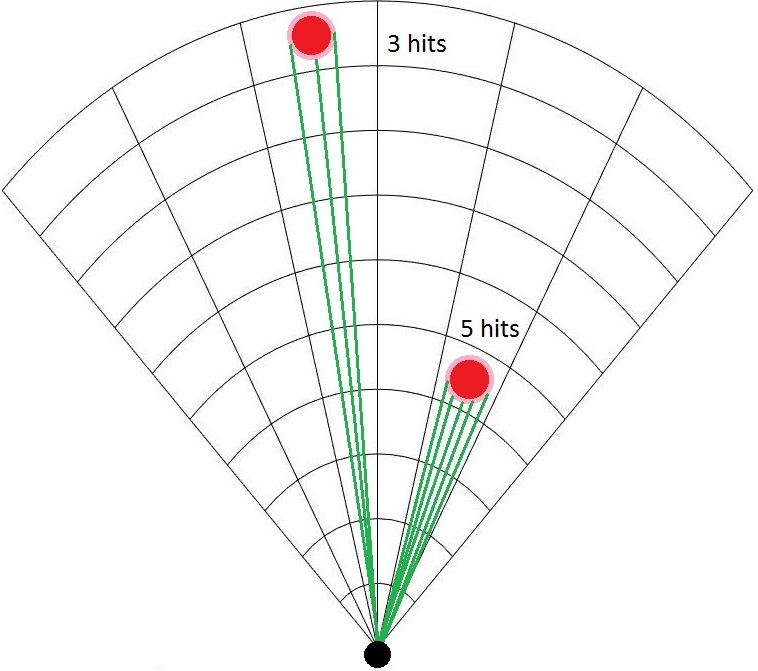
\includegraphics[width=0.7\textwidth]{\FIGDIR/P01CountOfLiDARHits}
    \caption{Different count of LiDAR hits on objects with same size but different distance from vehicle}
    \label{fig:P01CountOfLiDARHits}
\end{figure}

\section{Fusion of obstacle map with detected obstacles}
\noindent The concept of \emph{offline/online obstacle map} is mandatory in modern obstacle avoidance systems and increases the safety of trajectory planning. \emph{Deterministic} concept was considering only LiDAR reading or \emph{real-time reading} in general. The fusion of real time reading and obstacle map (prior knowledge) is required. Data fusion of these two sources is strongly depending on visibility property, because there are three basic scenarios:
\begin{enumerate}
    \item \emph{Dual detection} - the obstacle is marked on the map and detected by sensory system at some point of the time (deterministic concept works).
    \item \emph{Hindered vision} - the detected obstacles are hindering vision to map obstacle therefore map obstacle uncertainty arises (deterministic concept fails). 
    \item \emph{False-positive map} - map obstacle occupied space is visible by sensory system, but negative detection is returned. Therefore the map is giving \emph{false-positive} information.
\end{enumerate}
\noindent The second case is given in fig. \ref{fig:P02OvershadowedMapobstacle}, where map obstacle (blue circle) is overshadowed by three scanned obstacles (red circle). The visible space is denoted by green fill, the invisible space is denoted by gray fill. 


\begin{figure}[htbp]
    \centering
    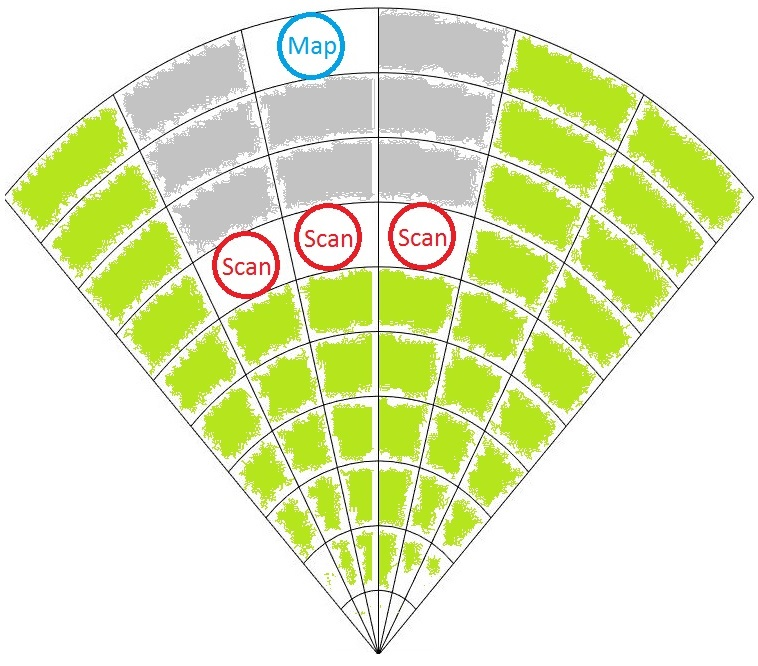
\includegraphics[width=0.7\textwidth]{\FIGDIR/P02OvershadowedMapobstacle}
    \caption{Overshadowed map obstacle by detected obstacles}
    \label{fig:P02OvershadowedMapobstacle}
\end{figure}


\subsection{Adversary/Intruder probability spread}
\noindent \emph{Adversarial behaviour} is first incorporation of moving obstacle. The Adversary is trying to destroy avoiding vehicle. Intruder concept will be used instead of adversary concept in this work. The \emph{intruder} vehicle (for short intruder) is in non-cooperative mode and is not trying to hurt our vehicle. The non-cooperative premise is given by current standard behaviour of small UAV vehicles. \emph{Minimal data set} which can extracted for any intruder consist from:
\begin{enumerate}
    \item\emph{Position} $\vec{p}\in\R^3$ - position of intruder in any transferable vehicle coordinate frame can be extracted and converted into \emph{avoidance coordinate frame}
    \item\emph{Heading (velocity)} $\vec{v}\in\R^3$ - heading with time parameter or velocity of intruder can be read or estimated trough various means. It must be converted into \emph{avoidance coordinate frame}.
    \item\emph{Uncertainty spreads} $\theta,\varphi,\dots$ - various spreads of uncertain intruder maneuverability.
\end{enumerate}

\noindent Example of intruder intersection without \emph{time of intersection} consideration is given in fig. \ref{fig:P03AdversaryProbabilitySpread}. The intruder initial position $\vec{p}$ at time of avoidance $t_i$ is denoted as green circle with 'A' letter. The intruder linear path approximation based on velocity $\vec{v}$ is denoted as middle green line. The spread of intruder maneuverability is given as outer green lines. The probability of intersection is denoted as green-orange-red cell fill, meaning is the red is high probability of intersection, orange is medium probability of intersection and green is low probability of intersection. 

\begin{figure}[htbp]
    \centering
    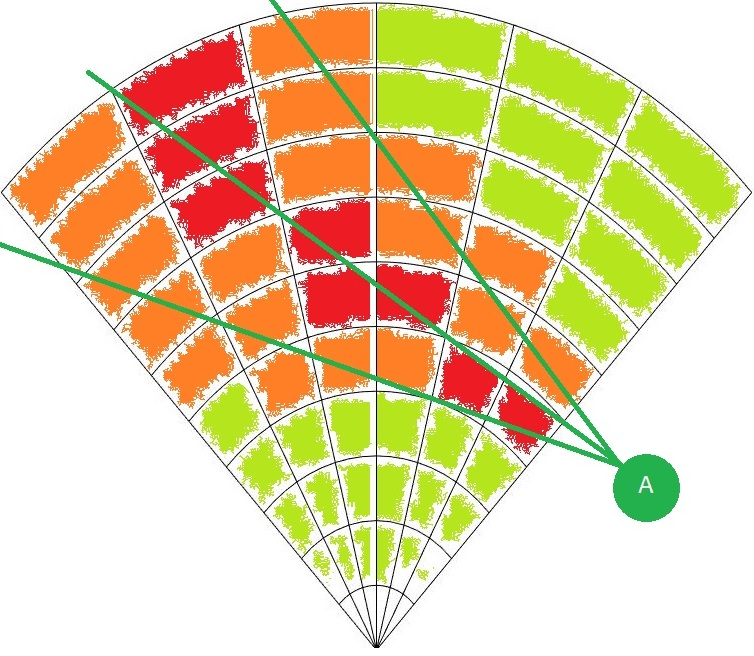
\includegraphics[width=0.7\textwidth]{\FIGDIR/P03AdversaryProbabilitySpread}
    \caption{Intruder vehicle collision probability along assumed trajectory with uncertain spread.}
    \label{fig:P03AdversaryProbabilitySpread}
\end{figure}

\subsection{Safety of passing trajectories}
\noindent Safety of passing trajectories is given by combined safety of passing cells. Each trajectory $\mathscr{T}(\vec{x},B)$ incorporated in reach set approximation $\mathscr{R}(\vec{x},t_i,t_{i+1})$ is passing trough ordered set of cells $\mathscr{C}\subset\mathscr{A}(t_i)$. The base safety rating of single cell $c_{i,j,k}\mathscr{C}$ can be expressed as product of cell visibility rating and inverted cell obstacle rating. Simply if cell is visible and probability of obstacle is low, cell is safe. \emph{Safe trajectory} is trajectory which have safe space along the path. The example of trajectories safety is given in fig. \ref{fig:P04SafetyOfPassingTrajectories}. The safety ratings of cell are given by red-orange-pink-green fills, where red denotes very low safety, orange denotes low safety, pink denotes medium safety, green denotes high safety. Blue trajectory is passing trough many unsafe cells and therefore overall safety is dangerous. Yellow trajectory is passing trough few cells with low and medium safety, therefore the choice of this trajectory is questionable. Green trajectory is passing only trough one cell with medium (pink) cell otherwise it passes trough all very safe cells, therefore its safe to chose this trajectory. The obstacle which caused such cell safety assessment is denoted as black filled circle with 'O' markings.

\begin{figure}[htbp]
    \centering
    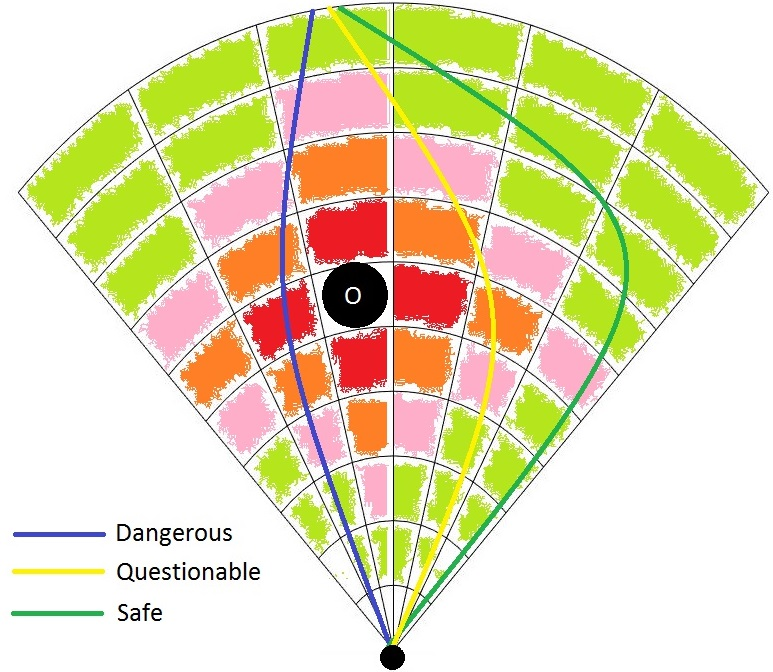
\includegraphics[width=0.7\textwidth]{\FIGDIR/P04SafetyOfPassingTrajectories}
    \caption{Trajectories leading to same destination with different safety ratings.}
    \label{fig:P04SafetyOfPassingTrajectories}
\end{figure}

\subsection{Addressed issues summary}
\noindent Following issues have been extracted of previously mentioned situations. they have been generalized in context of previous \emph{deterministic} approach, offline obstacle map, and intruder behaviour model.

\begin{enumerate}
    \item \textit{Model for intruder passing} - intruder can pass trough vehicle`s FOV at different times with different probability. There are multiple intruder behaviours which have not been accounted in previous approach, like intruder speed and heading uncertainty, intruder own maneuverability etc ...
    \item \textit{Multiple obstacle sources} - concept of visibility is mandatory for map and sensor reading obstacle fusion. The introduction of visibility needs to be done prior multiple source data fusion.
    \item \textit{Reachibility differentiation} - some cells in avoidance grid $\mathscr{A}(t_i)$ are more reachable than other, for example cell with one feasible trajectory has same reachability than cell with multiple leading trajectory.
    \item \textit{Decision making support} - some trajectories leading to same goal have different execution cost and different safety rating, this can be used as additional decision factor. For example framework can choose more expensive but safer trajectory to avoid.
    \item \textit{Obstacle size impact} - obstacle size can have impact on cell safety rating, in deterministic approach cell with one small obstacle have same safety rating than cell with big obstacle.
\end{enumerate}

\newpage
\section{Probabilities for trajectory and grid cell}
\noindent The preliminary analysis of scenarios and identified behaviours and impacts of probabilistic approach gives us an opportunity to identify specific track-able ratings for cell and trajectory artifacts. 
Each cell $c_{i,j,k}$ at avoidance time $t_i$ must have assessed this minimal set of probabilities:
\begin{enumerate}    
    \item \textit{Obstacle probability $P_O$} - determines the probability of obstacle encounter in given cell, obstacle probability is combination of various sources. Initial value of obstacle probability $P_O$ is assumed as 100 \%.
    \item \textit{Visibility $P_V$} -determines visibility of cell at time of avoidance $t_i$, portion of sight into cell space can be hindered by obstacles in front of cell.
    \item \textit{Reachibility $P_R$} - determines the maximum reachability like-hood for given cell based on passing trajectories. 
\end{enumerate}

\noindent Each trajectory $\mathscr{T}(x_0,B)\in\mathscr{R}(t_0,t_1,x_0)$ for each trajectory point $p_\mathscr{T}\in\left\{\mathscr{T}(x_0,B)\to\R^3\right\}$ must have assessed this minimal set of properties: 
\begin{enumerate}    
        \item \textit{Reachibility $P_R$} - determines reachability rating of given point $p_\mathscr{T}$.
        \item \textit{Feasibility of decision $P_D$} - determines next decision feasibility rating.
\end{enumerate}

\chapter{State of art}\label{03StateOfArt}
\noindent
Cooperative and non cooperative Sense and Avoid (SAA) systems are key enablers for Unmanned Aircraft (UAV) to routinely access non-segregated airspace \cite{spriesterbach2013unmanned}. Both cooperative and non-cooperative SAA systems are being developed to address this integration requirement.
\noindent
The SAA capability is defined as the automatic detection of possible conflicts by the UAV platform under consideration and performing avoidance maneuver tasks to prevent the identified collisions. An analysis of the available SAA candidate technologies and the associated sensors for both cooperative and non-cooperative SAA systems is presented in \cite{muraru2011critical}. Non-cooperative Collision Detection and Resolution (CD\&R) for UAV is considered as one of the major challenges that needs to be addressed \cite{lai2012see} for the insertion of UAVs in non-segregated air space. As a result, a number of non-cooperative sensors for the SAA system have been adopted. Light Detection and Ranging (LIDAR)is used for detecting, warning and avoiding obstacles for low-level flying \cite{sabatini2014lidar}.

An approach to the definition of encounter models and their applications to SAA strategies is presented in \cite{kochenderfer2008encounter} for both cooperative and non-cooperative scenarios.

Since 2014, there is a visible strong political support for developing rules on drones but regulations are not harmonized yet. The European Aviation Safety Agency (EASA) has been tasked to develop a regulatory framework for drone operations and proposals for the regulation of "low-risk" UAV operations. In achieving this, EASA is working closely with the Joint Authorities for Regulation of Unmanned Systes (JARUS) \cite{jarus2016regulations}.


\section{UAV motion model}
\noindent
This section strongly follows \cite{lee2011structure}.

\subsection{Continuous-time systems}\noindent
%This is very imprecise. A good notation is:
%1. u is the control function. It is a map from a time interval to \R^p, i.e., u:[0,T] \to %\R^p. Thus you could write u\in \C^p
%2. u(t) is the value (in \R^p) of the control function u. It is correct to write u(t)\in %\R^p

%You have to say what \C^p is. I guess that you mean the space of continuous functions. If this is the case, this specification is very unnatural since this space is too restrictive. Controls of interest usually have discontinuities.  More common is L^1 (space of integrable functions).

\noindent Consider a class of systems given by functions:
\begin{equation}
    \begin{split}
    S&: \vec{u}(t)  \to \vec{x}(\vec{x}_0,t) \\
    \vec{u}&(t): [0,T] \to \R^p \\
    \vec{u}&(t)\in \mathbb{R}^p , \vec{x}(t) \in \mathbb{R}^n \\
    \end{split}
\end{equation}
where $\vec{u}(t)$ and  $\vec{x}(\vec{x}_0,t)$ are a sets of continuous-time signals.
These are often called continuous-time systems because they operate on
continuous-time signals. Frequently, such systems can be defined by differential
equations that relate the input signal to the output signal.
A prototypical description of a controlled (there is a control input signal)
continuous-time system is:
\begin{equation}\label{eq:nonlinearsystem}
    \dot{x}(t) = f(t,x(t),u(t)), u(t) \in U(t)
\end{equation}
where $f:\mathbb{R}\times\mathbb{R}^n\times\mathbb{R}^p\to\mathbb{R}^n$
satisfies the conditions for existence
and uniqueness of the ordinary differential equation and $u$ is our control\cite{butcher1987numerical}.

\subsection{Discrete-time systems}
\noindent
\noindent Consider another class of systems given by functions
\begin{equation}\label{eq:Discretegenericuavmodel}
    \begin{split}
    S&: \vec{u}(k)  \to \vec{x}(k), \\
    k& \in \{0, t_s, 2.t_s, 3.t_s, \dots i.t_s\}, i \in \N^+\\
    \vec{u}&(k)\in \mathbb{R}^p , \vec{x}(k) \in \mathbb{R}^n\\
    \end{split}
\end{equation}
where $\vec{u}(k), \vec{x}(k)$ is a set of discrete-time signals. They can be represented by a function $f$ like $f:\{0, t_s, 2.t_s, 3.t_s, \dots i.t_s\} \to \R^n,  i \in \N^+$ where $t_s$ is sampling time and $i$ is discrete step \cite{shampine1997matlab}.

% REACH SETS
\section{Reach sets}\label{s:ReachSets}
\noindent
The reach set of a system described by a differential equation is the
set of all states that can be reached from an initial state within a given time
interval.
\noindent For general case consider the system described by equation (\ref{eq:nonlinearsystem}).

\begin{definition}[Reach set starting at a given point]\label{def:reachset01}
Suppose the initial position
and time $(\vec{x}_0, t_0)$ are given. The reach set $\mathscr{R}[\tau; t_0, \vec{x}_0]$ of system (\ref{eq:nonlinearsystem}) at time $\tau \ge t_0$, starting at position and time $(\vec{x}_0, t_0)$ is given by:
\begin{equation}\label{eq:basicReachSetDefinition}
    \mathscr{R}[\tau, t_0, \vec{x}_0] = \bigcup \{\vec{x}(\tau):\vec{u}(s)\in U(s),s \in (t_0,\tau]\}
\end{equation}
\end{definition}
\noindent Reach set starting at given set can be used to determine reach set in case of hybrid system input control switch and it is defined as follow:
\begin{definition}[Reach set starting at a given set]
The reach set at time $\tau > t_0$ starting from set $X_0$ is defined as:
\begin{equation}
    \mathscr{R}[\tau, t_0, X_0] = \bigcup \{R[\tau, t_0, \vec{x}_0]:\vec{x}_0 \in X_0\}
\end{equation}
\end{definition}

\noindent Reach set for adversarial behavior can be used to calculate possible escape routes from pursuer and it is defined as follow:
\begin{definition}[Reach set under adversarial behavior]
Consider now the case of adversarial behavior, for system $\dot{x}=u,u\in \mathbb{B}$.
where $u(t)$ is our control and $v(t)$ is adversary control which is independent of $u(t)$, let $w(t)=u(t)- \arg_{v(t)\in V(t)}\sup_{{x} \in x(t)} v(t)$, which represents worst possible input change in given state and time, then reach set for system is represented as:
\begin{equation}
    \mathscr{R}[\tau; t_0, \vec{x}_0] = \bigcup \{\vec{x}(\tau):\vec{w}(s) \in W(s),s \in (t_0,\tau]\}
\end{equation}

\end{definition}

\noindent Reach set under constraints are usable to define state constrained systems in terms of dynamics and technical capabilities.
\begin{definition}[Reach set under state constraints]
Suppose the initial position
and time $(\vec{x}_0, t_0)$ and $x$ constraints are given $x(t) \in \mathbb{A} \subset \R^n, \dot{x}(t) \in \mathbb{B} \subset \R^n$. The reach set $\mathscr{R}[\tau, t_0, \vec{x}_0]$ of system (\ref{eq:nonlinearsystem}) at time $\tau \ge t_0$, starting at position and time $(\vec{x}_0, t_0)$ is given by:
\begin{equation}
    \mathscr{R}[\tau, t_0, \vec{x}_0] = \bigcup \{\vec{x}(\tau):\forall s\in (t_0,\tau], x(s) \in \mathbb{A}, \dot{x}(s) \in \mathbb{B}, \exists u(s) \in U(s)\}
\end{equation}
\end{definition}


\section{Occupied space}
\noindent Occupied space representation is crucial in obstacle avoidance, this section introduces models and notations. Analytical geometry structures of sphere and ellipsoid are used to  determine closed occupied spaces.
\begin{definition}{Unit sphere (Unit ball) $\mathscr{B}(\vec{p},r)$} denotes occupied space in point $\vec{p} = [x_p,y_p,z_p]^T$ with radius $r$. Where point $\vec{b} = [x_b,y_b,z_b]$ belongs to sphere $\mathscr{B}(\vec{p},r)$ if and only if:
\begin{equation}
    (x_b-x_p)^2 + (y_b-y_p)^2 + (z_b-z_p)^2 \le r
\end{equation}    
\end{definition}
Definition of sphere $\mathscr{B}(\vec{p},r)$ is usually used to denote safety margin of vehicle $s_m$, where $s_m$ represents maximum radius to vehicle matter point from vehicle mass center. 
\begin{definition}{Spherical coating $\mathscr{C}(\vec{f}(\cdot),r)$} denotes occupied space of object which surface can be approximated by function $f(\cdot)$, with points of surface $\vec{p}=[x_p,y_p,z_p]^T\in\R^3$ and object inner points $\vec{i}=[x_i,y_i,i_p]^T\in \R^3$. Then spherical coating $\mathscr{C}(\vec{f}(\cdot),r)$ is defined as follows:
\begin{equation}
    \mathscr{C}(\vec{f}(\cdot),r) = \left\{\vec{b} \in \R^3: \vec{b}\in \bigcup_{\forall \vec{p} \in \vec{f}(\cdot)} \mathscr{B}(\vec{p},r), \nexists \vec{i}=\vec{b}  \right\}
\end{equation}
One can say that spherical coating is a closed,not compact set of points $\vec{b} = [x_b,y_b,z_b]$  where distance to closest surface point $\vec{p}$ is lesser or equal to coating radius $r$.    
\end{definition}
\noindent Calculation of spherical coating can be time consuming especially when surface function $\vec{f}(\cdot)$ is not smooth \cite{sommerville2016analytical}. Closest point problem has been formulated by Shamos \cite{shamos1975closest}.Closest point estimation with moving vehicle and with thick data flow can by solved by time optimal and deterministic approach, one of them have been presented by Bentley in \cite{bentley1980optimal}. Approach is based on closest point search in local planar coordinates which may be ideal for steam-line LiDAR data. 
Estimation of spherical coating is used in potential field avoidance methods. One most notable study was using spherical approximation based on obstacle center and mass distribution in space \cite{borenstein1991vector}. Potential field have their limitations in partially known environment, because it is hard to determine center of mass and mass distribution of obstacle from partial information \cite{koren1991potential}. Main source of object proportional estimation can be reused from camera based solutions like \cite{oberkampf1993iterative}. Other possible solution sources from fast clustering algorithms from Geographical Information Systems (GIS) for example \cite{zaiane2002clustering}.

\section{Movement automaton}\label{sec:movement automaton}
\noindent Movement automaton used as proxy between discrete command chain (movement chain) and control signal ($u(t)$). Movement automation is based on hybrid automaton.
\begin{definition} {Hybrid automaton $\mathscr{H}(Q,\R^n,f,\varphi,\rho)$} is well defined system representation consisting from following components.
\begin{equation}
    \begin{aligned}
        Q &\equiv \textnormal{set of discrete states}\\
        \R^n &\equiv \textnormal{continuous state-space} \\
        f: Q\times \R^n \to \R^n & \equiv \textnormal{vector field}\\
        \varphi:Q\times \R^n \to Q & \equiv \textit{discrete transition}\\
        \rho : Q\times \R^n \to \R^n & \equiv\textit{reset map}\\
    \end{aligned}
\end{equation}
Discrete state $q_i \in Q$ represents system current state and impacts system behavioural equation and state. Continuous state $[x(t),u(t)]\in \R^n$ represents  system state from physical viewpoint (values of state variables and inputs in continuous space $\R^n$). Vector field $f$ assign to each discrete state $q_i \in Q$ system behavioral function $\dot{x} = f(x,u)$. Discrete transition $\varphi$ defines conditions to transit between two different states. Reset map $\rho$ defines system state or input change on reset conditions.
\end{definition} 

\begin{definition}{Trajectory primitive $\hat{t}(x_0,t_0,t_1)$} is defined on given time interval $(t_0,t_1]$ for system $\dot{x} = f(x,u)$ with initial state $x_0$ at $t_0$ and final state $x_1$ at $t_1$ as follow:
\begin{equation}
    \hat{t}(x_0,t_1,t_1) = \left\{ x\in\R^n: x = \Phi(t_0,\tau,x_0), \tau \in (t_0,t_1] \right\}
\end{equation}
Trajectory primitive can be viewed as ordered set of system trajectory positions, this set is infinite continuous and flat.    
\end{definition}

\begin{definition}{Trajectory equivalence.}
Let $\mathscr{T}$ be trajectory defined as ordered sequence of countable trajectory primitives:
\begin{equation}
    \mathscr{T} = \left\{ \bigcup_{i=0}^n \hat{t}_i(x_i,t_i,t_{i+1}) \right\}
\end{equation}
Trajectory $\mathscr{T}$ is time independent and contains at leas one trajectory primitive. Trajectory $\mathscr{T}_\alpha$ consist from $m\ge 1$ trajectory primitives and its smooth and continuous. Trajectory $\mathscr{T}_\beta$ consist from $n \ne m$ primitives and its smooth and continuous.  Trajectories $\mathscr{T}_\alpha \equiv \mathscr{T}_\beta$ if and only if:
\begin{equation}
    \forall x_i \in \mathscr{T}_\alpha \exists y_i \in \mathscr{T}_\beta: x_{i+1} \equiv y_{i+1}, i \in {0\dots k}
\end{equation}
Where $x_i$ and $y_i$ is i-th point of trajectorries in state space $\R^n$.
\end{definition}

\noindent Trajectory primitives and trajectory equivalence have been defined, therefore movement primitives and movement can be defined.

\begin{definition}{Movement primitive $p$} 
for system $\dot{x} = f(x,u)$ and time interval $(t_i,t_{i+1}]$ there is defined continuous input signal $u(t)$.
\begin{equation}
    p_i = u(t), t\in (t_i,t_{i+1}]
\end{equation}
\end{definition}

\noindent Movement primitives can be chained to give smooth input signal. if there is movement primitive $p_1$ and movement primitive $p_2$ they can be chained on time $\tau$ when $u_1(\tau) = u_2(\tau)$, therefore system state can be also chained $x_1(\tau) = x_2(\tau)$.
\begin{definition}{Movement m(t)} is defined as chain of movement primitives $\{p_1,p_2,\dots,p_n\}$. Movement is smooth function with existing derivation. 
\end{definition}
\noindent Movement is main building block of movement automaton, movement is defined by movement type and its duration, movement switching is possible when execution time allows movement chaining. Movements can be separated into two categories:
\begin{enumerate}
    \item \textit{Stationary movement} - movement signal is constant during time of movement execution
    \item \textit{Dynamic movement} - movement signal is evolving during time of movement execution.
\end{enumerate}
\begin{definition} {Movement automaton $\mathscr{MA}$}\label{def:movementAutomaton} for system defined by dynamics $\dot{x} = f(x,u)$ is a structure defined as follow:
\begin{equation}
    \begin{aligned}
    M&\equiv\textnormal{set of movements}\\
    u:M\times\R\to\R^m&\equiv\textnormal{input function evolution}\\
    \varphi:M\times M \times \R&\equiv\textnormal{movement transition map}\\
    B=M\times\R^2&\equiv\textnormal{movement buffer}\\
    \end{aligned}
\end{equation}
Movement $m_i\in M$ can be stationary or dynamic. Each movement in movement buffer has assigned duration $(t_i,t_{i+1}]\in\R^2$. Input function evolution $u(B,t)$ defines input evolution in given execution time $t = \tau+t_0, \tau\in(t_0,t_1]$.
Each movement $m_i$ in movement automaton $\mathscr{MA}$  is compliant with following rules:
\begin{enumerate}
    \item Each movement $m_i(t_{i},t_{i+1})$ has non zero duration.
    \item At switching time $\tau$ between movements $m_i$ and $m_{i+1}$, input function $u_i(\tau + t_i) = u_{i+1}(0)$.
    \item Each dynamic movement should be linking two static movement and vice-versa.
\end{enumerate}
\end{definition}

\subsection{Prediction stability of Movement Automaton}\label{s:maConvergence}
\noindent Because Movement automaton $\mathscr{MA}$ is abstract level control realized trough \textit{open loop hybrid automaton}, infinite receding horizon is questionable. This fact impacts the prediction reliability. This subsection formulates \textit{prediction horizon of movement automaton}.

\begin{definition}{Movement automaton $\mathscr{MA}$ prediction stability}\label{def:maPredictionStability}
For system $\dot{x}=f(x,\mathscr{MA})$ and predictor $\dot{\hat{x}}=f(\hat{x},\mathscr{MA})$ with separable nonlinear state $h(\cdot)$ and input transformation $g(\cdot)$ functions. With initial condition $x(t_0)=\hat{x}(t_0)=x_0$ and finite execution time $t\in[t_0,t_1]$. Prediction deviation $x(t)-hat(x)(t)$ stays in unit ball defined by:
\begin{equation}
    \mathscr{B}(x(t)-\hat{x}(t))= \left\{y\in\R^n:y=x(t)-\hat{x}(t),\norm{y}\le\rho\right\}
\end{equation}
\end{definition}

\begin{dokaz}
Let $\dot{x}=f(x,\mathscr{MA})$ be continuous time system, with state $x\R^n$ and control with movement automaton $\mathscr{MA}$. Input function $u(t)$ for movement buffer $B=\{m_1(t_1),\dots,m_i(t_i)\}$ is interpreted as chained input function:
\begin{equation}\label{eq:maTranslation}
    u(t)=
    \begin{cases}
        u(m_0,m_1,t_0,t_1)&:\textnormal{for } m_1(t_1)\\
        \vdots&\\
        u(m_{i-1},m_{i},t_{i-1},t_{i})&:\textnormal{for } m_i(t_i)
    \end{cases}
\end{equation}
\noindent Input function $u(t)$ (\ref{eq:maTranslation}) is smooth and differentiable as given by movement automaton $\mathscr{MA}$  definition (def. \ref{def:movementAutomaton}.). Let $w(t)$ be state noise function with boundary $\xi_w\in\R-\{\infty\}$, $v(t)$ input noise function with boundary $\xi_v\in\R-\{\infty\}$ and $\hat{x}(t)$ predicted state for movement chain $B=\{m_1(t_1),\dots,m_i(t_i)\}$. We can define function $V(t)$ as follow:
\begin{equation}
    V(t) = \frac{1}{2} (x(t)-\hat(x){t})^T\text{I}(x(t)-\hat(x)(t)) = (x(t)-\hat{x}(t))^2
\end{equation}
\noindent Given function can be derived by time $t$: 
\begin{equation}
    \dot{V}(t) = x(t)-\hat(x)(t)
\end{equation}
\noindent Controlled system with state $w(t)$ and input noise $v(t)$, where input and state are separable:
\begin{equation}
    \dot{x}=f(x,\mathscr{MA}) = g(x(t)+ w(t)) + h(u(t)+ v(t))
\end{equation}
\noindent Predicted system equation:
\begin{equation}
    \dot{\hat{x}}=f(\hat{x},\mathscr{MA}) = g(\hat{x}(t)) + h(u(t))    
\end{equation}
\noindent Therefore $\dot{V}$ is equal to:
\begin{equation}
    \begin{split}  
    \dot{V}(t) &= (g(x(t)+ w(t)) + h(u(t)+ v(t))) - (g(\hat{x}(t)) + h(u(t)))\\
               &=  g(w(t)) + h(v(t))
    \end{split}
\end{equation}
\noindent Member $g(x(t)-\hat{x}(t))$ is equal to zero, because of the premise that predicted $\hat{x}$ and real state $x$ are equal without state $w(t)$ and input noise $v(t)$ noise. Let us bound $g(w(t))$, boundary is straightforward in this case, because state noise $w(t)$ is bounded by $\xi_w$. Boundary is given as:
\begin{equation}
    \norm{g(w(t))} \le \norm{g(_{sup}(w(t)))} \le \norm{g(\xi_w)} \le \rho_w,\quad \rho_w\in\R^+-\{\infty\}
\end{equation}
\noindent Bounding member $h(v(t))$ will be problematic due to mapping function (\ref{eq:maTranslation}). Introducing input noise to movement automaton mapping function will cause input noise to be characterized like this:
\begin{equation}
    u(t)-\hat{u}(t)=\left(
    \begin{cases}
        u(m_0,m_1,t_0,t_1)+v_1(t)&\\
        \vdots&\\
        u(m_{i-1},m_{i},t_{i-1},t_{i})+v_i(t)^i&
    \end{cases}
    \right) -\left(
    \begin{cases}
        \hat{u}(m_0,m_1,t_0,t_1)&\\
        \vdots&\\
        \hat{u}(m_{i-1},m_{i},t_{i-1},t_{i})&
    \end{cases}
    \right) 
\end{equation}
\noindent This can be simplified to:
\begin{equation}
    \sum_{l=0}^{i} v_l(t)^l, \quad i\in\R^{+}-\{0,\infty\}
\end{equation}
\noindent So for case of input noise $v(t)$ member $h(v(t))$ of $\dot{V}(t)$ can be bounded like follow:
\begin{equation}
    \norm{h(v(t))} \le \norm{h(_{sup}\sum_{l=0}^{i} v_l(t)^l)}\le \norm{h(\xi^i)} \le \rho_v \quad \rho_v\in\R^+-\{\infty\}
\end{equation}
\noindent Where $i$ is finite count of movements in movement automaton $\mathscr{MA}$ buffer $B$, $i=|B|$. This parameter is cumulative which is given by member $\norm{h(_{sup}\sum_{l=0}^{i} v_l(t)^l)}$, but it is bounded by $\norm{h(\xi^i)}$. One can define boundary as follow:
\begin{equation}
    \norm{\dot{V}(t)} \le \rho_w + \rho_v = \rho, \quad \rho\in\R^+-\{\infty\}
\end{equation}
\noindent With boundary defined for derivation of $V(t)$ one can define boundary for $V(t)$ like follow for time of prediction $t_0$ and time of movement buffer execution end $t_i$:
\begin{equation}
    \norm{V(t)} \le \int_{t_0}^{t_i} \norm{\dot{V}(t)}\quad \text{d}t \le \int_{t_0}^{t_i} \rho \quad\text{d}t = \rho(t_i-t_0)
\end{equation}
\end{dokaz}
\subsection{Lyapunov stability of Movement Automaton}\label{s:maLyapunov}
\noindent It has been proven that system with movement automaton is stable in terms of finite receding horizon prediction. There is still open issue of \textit{Lyapunov stability}. To prove Lyapunov stability one needs to construct tracking problem of waypoint. Let say that system initial state $x(t_0)\in \mathscr{B}_s \subset \R^n$ is unit ball where system $\dot{x} = g(x) + h(u)$ is trying to reach equilibrium point $\hat{x}(t_i)$. Equilibrium point is predicted state $\hat{x}$ at final time of movement automaton $\mathscr{MA}$ buffer execution $t_i$. Then region of attraction $\mathscr{B}(\hat{x}(t_i),\rho)$, where $\hat{x}(t_i)$ is center of unit ball and $\rho$ is prediction deviation boundary at time $t_i$ given by definition (def. \ref{def:maPredictionStability}). Let us define system $y$ for tracking problem with equilibrium point $x(t_i)$ and initial state $x(t_0)\in\mathscr{B}_s$ for finite time period $t_\in[t_0,t_i]$
\begin{equation}
    y = {x}(t)-\hat{x}(t_i), \quad x(t_0)\in\mathscr{B}_s\subset\R^n, 
\end{equation}
\noindent It is obvious that region of attraction $\mathscr{B}(\hat{x}(t_i),\rho)$, is subset of $\mathscr{B}_s$. Let us define simple Lyapunov function $V(y)$ like follow:
\begin{equation}
    V(y) = \frac{1}{2}y^Ty = \frac{1}{2}\sum_{l=1}^n\left(x_l(t)^2-\hat{x}_l(t_i)^2\right)
\end{equation}
\noindent With derivation in time given by equation:
\begin{equation}
    \dot{V}(y)= \sum_{l=1}^n \frac{\partial V(y)}{\partial y_l}
\end{equation}
\noindent Now lets check second Lyapunov method stability conditions for $y$:
\begin{enumerate}
    \item $V(0)=0$ - this condition is valid, because Lyapunov function is 0 at equilibrium point $\hat{x}(t_i)$.
    \item $V(y) < 0, \forall y\in\mathscr{B}_s-\{0\}$ - this condition is valid, because $\frac{1}{2}\norm{y}>0,\forall y\in\mathscr{B}_s-\{0\}$.
    \item $\dot{V}(y)<0$ or $\dot{V}(y)\le0$ - convergence criterion is fully satisfied in case of no existing obstacle, because avoidance framework converges to goal waypoint exponentially fast.
\end{enumerate}
\noindent Convergence condition $\dot{V}(y)<0$ is not guaranteed in term of obstacle avoidance, because in some cases $\dot{V}(y)>0$ while avoiding enormous obstacle. Movement automaton $\mathscr{MA}$ is exponentially or at least asymptotic stable in terms of Lyapunov stability, within region of attraction $\mathscr{B}(\hat{x}(t_i),\rho)$. Obstacle avoidance framework is can be or can not be Lyapunov stable depending on obstacle set $\mathscr{O}$. Reachibility of waypoint $\hat{x}(t_i)$ is determined by system reachibility set $\mathscr{R}$.


\section{LiDAR}
\noindent LiDAR (Light Detection And Ranging) is active form of remote sensing: information is obtained from a signal which is sent from a transmitter and reflected by a target, and detected by a receiver back at the source. Following types of information can be obtained:
\begin{enumerate}
\item \textit{Range to target} - topographic LiDAR or laser altimeter.
\item \textit{Chemical properties of target} - differential absorption LiDAR.
\item \textit{Velocity of target} - Doppler LiDAR.
\end{enumerate}

\noindent Chemical properties of target are out of scope. Velocity of  target seems as interesting property to investigate, but this type of LiDAR is usually used for meteorological measurements of wind currents \cite{martin2011meteorological}. Extended research in LiDAR as obstacle detection sensor has been executed by research group around Sabatini \cite{sabatini2014lidar} and Ramasy \cite{ramasamy2016lidar}. 

LiDAR output is represented as point cloud it is described by following definition.
\begin{definition}[Scanned point and Point-cloud]
Consider viewpoint $v$ as origin of $\R^3$ space in 
Let point $p \in P$ be defined in polar coordinates:
\begin{equation}
    p= [ d, \theta, \varphi, t ]^T
\end{equation}
Where $d$ is distance to scanner, $\theta$ is horizontal angle from origin, $\varphi$ is vertical angle to origin, $t$ is time of retrieval.\\

\noindent Point-cloud is set of points scanned in small enough time-frame, based on processing raw point data it can have following representations:
\begin{enumerate}
\item Local point-cloud - position of sensor is used as origin of space and points can be represented in orthogonal or planar representation. 
\item Global point-cloud -global position of sensor is used as reference to calculate global position of points.
\end{enumerate}
\end{definition}

Point-cloud is usually addressed as \textit{raw point-cloud} in case if its represented in Local planar coordinates. Other forms of point cloud require further processing and they are not feasible for real time obstacle detection and avoidance \cite{chen2007airborne}.

\begin{figure}[H]
    \begin{subfigure}{0.5\textwidth}
    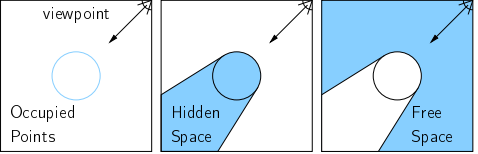
\includegraphics[width=0.9\linewidth]{\FIGDIR/10_Lidar_sets1.PNG} 
    \caption{Space type definitions}
    \label{fig:Spacetypes}
    \end{subfigure}
    \begin{subfigure}{0.5\textwidth}
    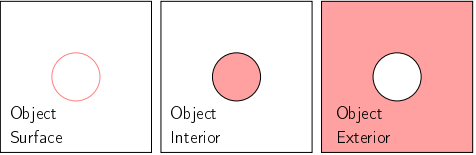
\includegraphics[width=0.9\linewidth]{\FIGDIR/11_Lidar_sets2.PNG}
    \caption{Object properties definitions}
    \label{fig:ObectProperties}
    \end{subfigure}
    \caption{Six spaces of interest \cite{yapo2008probabilistic}}
    \label{fig:Spaces of interests}
 \end{figure}
 
\noindent  Because of real-time obstacle avoidance it is necessary to introduce following terminology:
\begin{enumerate}
    \item \textit{Occupied points} - points which have been detected by LiDAR (also addressed as visible points).
    \item \textit{Hidden space} - space which is hidden behind occupied points, from viewpoint it is uncertain what is in that space. 
    \item \textit{Free space} - space which is visible from viewpoint and it is not occupied by known objects.
    \item \textit{Object surface} - detected and undetected object surface
    \item \textit{Object interior} - occupied space by object.
    \item \textit{Object exterior} - free space around known objects.
\end{enumerate}
Existing method for space segregation \cite{yapo2008probabilistic} can yeld to following definition.
\begin{definition}[Accessible space]\label{def:accessibleSpace}
    Consider known space $S$ as space explored by sensor (it can have different viewpoint along previous 3D trajectory).
    Intersection between \textit{object exterior} $S_E$ and \textit{free space}$S_F$ gives us \textit{Accessible space}.
    \begin{equation}
        S_A = S_E \cap S_F
    \end{equation}
\end{definition}
 
 \noindent Accessible space $S_A$ (\ref{def:accessibleSpace}) is our bordering limitation for reachable space of system $R(\tau,t_0,\vec{x_0})$ (def. \ref{def:reachset01}.); 

 
\section{Complements of algebra}

\noindent 3D Cartesian space gives us an x, y, and z axis (describing position based on horizontal placement, vertical placement, and depth respectively). The coordinates for any point within this space are shown as a tuple $(x,y,z)$. Coordinate system used this work will be viewed as right-handed system (thumbs points at positive direction of x-axis, index finger is pointing to positive direction of y-axis, then positive  direction of z axis is shown by remaining fingers).

Euler have worked on universal rotation theorem which was presented in \cite{euler1775formulae}. Rigid body dynamics and rotation matrices have been proposed in book by Schaub \cite{schaub2003analytical}. Local coordinates are used, where plane center of gravity is used as center point and plane heading is oriented to X axis. This local coordinate system is called Euler Normalized Unit-frame (ENU). Rotation matrices are used to transform between two displaced coordinate systems. Roll angle $\alpha$ rotation is defined around X-axis by matrix (\ref{eq:rollTransformationMatrix}) on YZ-plane. Pitch angle $\beta$ rotation matrix is defined around Y-axis by matrix (\ref{eq:pitchTransformationMatrix}) on XZ plane. Yaw angle $\gamma$ rotation matrix is defined around Z axis by matrix (\ref{eq:yawTranformationMatrix}) on XY plane.

\begin{equation}\label{eq:rollTransformationMatrix}
    R_{YZ} = R_\alpha =
    \begin{bmatrix}
        1 & 0 & 0\\
        0 & \cos(\alpha) & -\sin(\alpha)\\
        0 & \sin(\alpha) & \cos(\alpha)
    \end{bmatrix}
\end{equation}
\begin{equation}\label{eq:pitchTransformationMatrix}
    R_{XZ} = R_\beta =
    \begin{bmatrix}
        \cos(\beta) & 0 & \sin(\beta)\\
        0 & 1 & 0\\
        -\sin(\beta) & 0 & \cos(\beta)
    \end{bmatrix}
\end{equation}
\begin{equation}\label{eq:yawTranformationMatrix}
    R_{XY} = R_\gamma = 
    \begin{bmatrix}
        \cos(\gamma) & -\sin(\gamma) & 0 \\
        \sin(\gamma) & \cos(\gamma) & 1 \\
        0 & 0 & 1
    \end{bmatrix}
\end{equation}
Final rotation matrix in XYZ ordered space is given by equation(\ref{eq:xyzspaceRotationMatrix}).
\begin{equation}\label{eq:xyzspaceRotationMatrix}
    \begin{aligned}
        R_{XYZ}  =& R_{\alpha\beta\gamma} =  R_{XY} * R_{XZ} * R_{YZ} = R_\gamma * R_\beta *R_\alpha\\
         =& 
         \small
         \begin{bmatrix}
            \cos\beta\cos\gamma & \cos\gamma\sin\alpha\sin\beta - \cos\alpha\sin\gamma & \sin\alpha\sin\gamma + \cos\alpha\cos\gamma\sin\beta \\
            \cos\beta\sin\gamma & \cos\alpha\cos\gamma + \sin\alpha\sin\beta\sin\gamma & \cos\alpha\sin\beta\sin\gamma - \cos\gamma\sin\alpha \\
            -\sin\beta & \cos\beta\sin\alpha & \cos\alpha\cos\beta 
         \end{bmatrix}
         \normalsize
    \end{aligned}
\end{equation}
To keep solution numerically stable and rotations numerically stable gimbal lock prevention is necessary \cite{kramer1977gyro}. Gimbal lock occurs when one of matrices (\ref{eq:rollTransformationMatrix}, \ref{eq:pitchTransformationMatrix}, \ref{eq:yawTranformationMatrix}) is singular or final matrix for XYZ rotation is singular (\ref{eq:xyzspaceRotationMatrix}). Gimbal lock leads to loose of one or more degree of freedom, depending on rank and space dimension of singular matrix. To prevent gimbal lock it is necessary to introduce mechanism to check if rotation matrix is regular. For this purpose normative reset function is introduced:
\begin{equation}
    \left [ \alpha, \beta ,\gamma \right ]^T = f(t,\alpha^-,\beta^-,\gamma^-), \quad \textnormal{norm}(R_{\alpha\beta\gamma})=3
\end{equation}
Function resets yaw $\gamma$ or roll $\alpha$ angle to initial position to keep degree of rotation matrix. Simpler but not fault tolerant solution is to keep angles $\alpha,\beta,\gamma, \in \left (  -\pi,\pi\right ]$ range.

\subsection{Transformation between coordinate systems}
\noindent Polar coordinate system represents point in form of vector $[distance$, $angle_{horizontal}$, $angle_{vertical}]$, which is ideal for representation of LiDAR scanned point, because usually total point distance andpair of angles are returned. Using most common LiDAR with horizontal rotation $\theta$ and vertical mirror inclination $\varphi$, one can define planar coordinate $p_{planar} = [d_{xyz},\theta,\varphi]$ which is dual to Cartesian coordinate $p_{cartesian} = [x,y,z]$. If rotation angles are forced to stay as $\theta,\varphi\in(-\pi,\pi]$ transformation function is bijection.

Transformation from planar to Cartesian representation is defined by following series of functions (\ref{eq:cpt01}, \ref{eq:cpt02},\ref{eq:cpt03}, \ref{eq:cpt04}).
\begin{equation}\label{eq:cpt01}
    d_{xy} = \cos\varphi.d_{xyz}
\end{equation}
\begin{equation}\label{eq:cpt02}
    z = \sin\varphi.d_{xyz}
\end{equation}
\begin{equation}\label{eq:cpt03}
    y = \sin\theta.d_{xy}
\end{equation}
\begin{equation}\label{eq:cpt04}
    x = \cos\theta.d_{xy}
\end{equation}
Transformation from Cartesian to planar representation is defined by following series of functions (\ref{eq:cpt05}, \ref{eq:cpt06},\ref{eq:cpt07}, \ref{eq:cpt08}).
\begin{equation}\label{eq:cpt05}
    d_{xyz} = \sqrt{x^2+y^2+z^2}    
\end{equation}
\begin{equation}\label{eq:cpt06}
    d_{xy} = \sqrt{x^2+y^2}    
\end{equation}
\begin{equation}\label{eq:cpt07}
    \theta = \arctan\frac{y}{x}
\end{equation}
\begin{equation}\label{eq:cpt08}
    \varphi= \arctan\frac{z}{d_{xy}}
\end{equation}

\begin{definition}{Global coordinate system $\mathscr{X}_\mathscr{G}$}\label{def:globalCoordinateSystem}
    takes as center $c_{\mathscr{G}0}$ well known point (for example center of geo-reference model in GNSS systems) every reference distance, plane or angle is calculated taking this center to mind.
\end{definition}
\begin{definition}{Local coordinate system $\mathscr{X}_\mathscr{L}$}\label{def:localCoordinateSystem}
    takes as center $c_{\mathscr{L}0}$ frame of vehicle and can be changing position and orientation in global coordinate frame $\mathscr{X}_\mathscr{G}$.
\end{definition}
\begin{definition}{Global position of planar obstacle $o_i\in\mathscr{O}_{3D}$.}\label{def:globalObstaclePosition3D}
    Let $o_i = [d_o, \theta_o, \varphi_o]^T$ be planar position of obstacle $o_i$ in local coordinate frame of vehicle with global Cartesian position $[x,_v,y_v,z_v]^T$ and normalized orientation angles $[\alpha_v,\beta_v,\gamma_v]$.\\
    Then Cartesian position of obstacle $oi$, $[x_o,y_o,z_o]^T$  in local coordinate frame is given by transformation functions $x_o$ (\ref{eq:cpt04}), $y_o$ (\ref{eq:cpt03}), $z_o$ (\ref{eq:cpt02}).\\ 
    Global  position of planar obstacle $oi$, $[x_g,y_g,z_g]^T$ is given by following equation:
    \begin{equation}
        \begin{bmatrix}
            x_g\\y_g\\z_g
        \end{bmatrix}
        =
        \left [
            R_{XYZ}(\alpha_v,\beta_v,\gamma_v)
            \begin{bmatrix}
                x_o\\y_o\\z_o
            \end{bmatrix}
            +
            \begin{bmatrix}
                x_v\\y_v\\z_v
            \end{bmatrix}
        \right ]
    \end{equation}    
\end{definition}

\begin{definition}{Local position of global coordinate $[x_g,y_g,z_g]^T\in\R^3$.}\label{def:globalToLocal}
    Let there be vehicle with global Cartesian position $[x,_v,y_v,z_v]^T$ and normalized orientation angles $[\alpha_v,\beta_v,\gamma_v]$. in global coordinate frame $\mathscr{X}_\mathscr{X}$.\\
    Then local Cartesian coordinate position $[x_l,y_l,z_l]^T$ of point $[x_g,y_g,z_g]^T$ is given by following equation:
    \begin{equation}
        \begin{bmatrix}
            x_l\\y_l\\z_l
        \end{bmatrix}
        =
        \left [
            R_{XYZ}(-\alpha_v,-\beta_v,-\gamma_v)
            \left (
            \begin{bmatrix}
                x_g\\y_g\\z_g
            \end{bmatrix}
            -
            \begin{bmatrix}
                x_v\\y_v\\z_v
            \end{bmatrix}
            \right )
        \right ]
    \end{equation}
    Local planar position is given as $[d_l, \theta_l,\varphi_l]$, where $d_l$ is given by (\ref{eq:cpt05}), $\theta_l$ is givent by (\ref{eq:cpt07}). $\varphi_l$ is given by (\ref{eq:cpt08}), where $[x_l,y_l,z_l]$ are used as local coordinates.
\end{definition}

\subsection{Planar surface calculation}
\noindent The problem is to calculate intersected surface $dA$ of ball subsurface defined by radius $r$, horizontal span $\phi$ and vertical span $\theta$. From clasicall mechanics one can formulate problem as given by figure \ref{fig:80BallSpan}. The intersection plot is in figure \ref{fig:81BallSpan2}.
\begin{figure}[H]
    \centering
    \begin{subfigure}[H]{0.3\textwidth}
        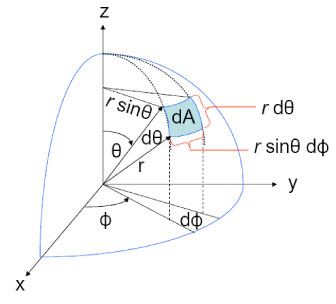
\includegraphics[width=\textwidth]{\FIGDIR/80BallSpan.jpg}
        \caption{Notation}
        \label{fig:80BallSpan}
    \end{subfigure}
    \begin{subfigure}[H]{0.3\textwidth}
        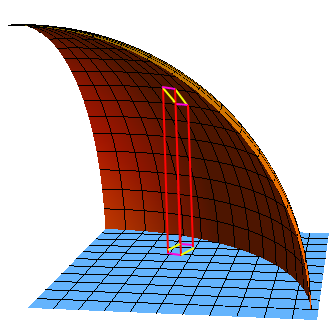
\includegraphics[width=\textwidth]{\FIGDIR/81BallSpan2.png}
        \caption{Plot}
        \label{fig:81BallSpan2}
    \end{subfigure}
    \caption{Planar surface calculation notation and plot}
    \label{fig:BallSpanNOTPLOT}
\end{figure}

\noindent One can use first fundamental form to determine the surface area element. Recall that this is the metric tensor, whose components are obtained by taking the inner product of two tangent vectors in planar space $g_{i,j}= X_i \cdot X_j$, for tangent vectors $X_i$, $X_j$. Following identification for the components of metric tensor will be used:
\begin{equation}\label{eq:metricTensorIdentification}
    g_{ij}=
    \begin{bmatrix}
        E&F\\
        F&G
    \end{bmatrix}
\end{equation}

\noindent Where $E=<X_u,X_u>$, $F=<X_u,X_v>$, and $G=<X_v,X_v>$. Lagrange`s identity can be used , which tells us that the squared area of a parallelogram in space is equal to the sum of the squares of its projections onto the Cartesian plane:
\begin{equation}\label{eq:CartesianProjectionIdentity}
    |X_u \times X_v|^2 = |X_u|^2|X_v|^2 - \left(X_u\cdot X_v\right)^2
\end{equation}

\noindent Given example is displayed in figure \ref{fig:81BallSpan2}. The area element is given as:
\begin{equation}\label{eq:squareElementSurfaceDerivation}
    \begin{aligned}
    \text{d}A &= |X_u \times X_v| \quad\text{d}u\text{d}v \\
    & = \sqrt{\left||X_u|^2|X_v|^2 - \left(X_u\cdot X_v\right)^2\right|}\quad \text{d}u\text{d}v\\ 
    & = \sqrt{EG-F^2} \quad \text{d}u\text{d}v
    \end{aligned}
\end{equation}

\noindent We will find tangent vectors via the usual parametrization which give, $X(\phi,\theta)$ = $[r \cos\phi\sin\theta,$ $r\sin\phi\sin\theta,$ $r\cos\theta]$, so that tangent vectors are simply defined as:
\begin{equation}\label{eq:tangentVectorsForPlanarSurface}
    \begin{aligned}
        X_\phi &= [-r\sin\phi\cos\theta,r\cos\phi\sin\theta,0]\\
        X_\theta &=[-r\cos\phi\sin\theta,r\sin\phi\cos\theta,-r\sin\theta]
    \end{aligned}
\end{equation}

\noindent Computing the elements of the first fundamental form gives us:
\begin{equation}
    E = r^2\cos^2\theta,\quad F=0,\quad G=r^2
\end{equation}

\noindent Thus final difference is given as:
\begin{equation}\label{eq:finalCellSquare}
    \text{d}A=\sqrt{r^4\cos^2}\quad \text{d}\theta\text{d}\phi = r^2 \cos\theta\quad \text{d}\theta\text{d}\phi
\end{equation}

\chapter{Probabilistic approach}\label{ch:04ProblemFormulation}
\noindent
Given a partial obstacle map, a mission plan, and a small UAV equiped with ADS-B and LiDAR sensor a safe approach to real-time obstacle avoidance with a small computational footprint compatible with the low computational power available in small UAVs. The main application consists of terrain and intruder avoidance for low altitude flights. Following assumption holds:
\begin{enumerate}
  \item There is a obstacle database charting some known obstacles prior the flight.
  \item There is possibility of non-adversarial and non-cooperative intruders.
  \item Estimates of the state of the UAV are available.
  \item The operational space does not contain 'traps' such as caves. 'Traps' arise because the field of view of the LiDAR does not include the whole space surrounding the UAV.
  \item There is a mission plan for the UAV consisting of waypoints which are reachable with vehicle dynamics.
\end{enumerate}
\noindent

\section{Simple plane model}\label{sec:3DsimplisticplaneModel}
\noindent For avoidance theorem formulation in three dimensional space simplified rigid body kinematic model will be used. This model have decoupled roll, yaw and pitch angles which enables to provide simpler and more clean control (e.g movements can be simplified). 

\begin{equation}\label{eq:simple3dStatevector}
    \vec{x} = \left [ x_v,y_v,z_v,\alpha_v,\beta_v,\gamma_v \right ]^T
\end{equation}
State vector (\ref{eq:simple3dStatevector}) defined as positional state in euclidean position in right-hand euclidean space, where $x_v, y_v,z_v$ states, for latitude, longitude and altitude. Orientation angles for vehicle are $\alpha\beta,\gamma$ for roll, pitch, yaw angle.
\begin{equation}\label{eq:simple3dInputVector}
    \vec{u} = \left [ v, \omega_{\alpha_v}, \omega_{\beta_v},\omega_{\gamma_v}\right ]^T
\end{equation}
Input vector (\ref{eq:simple3dInputVector}) is defined as frontal velocity of vehicle $v$,orientation change in main axes as angular speed $\omega_{\alpha_v},\omega_{\beta_v},\omega_{\gamma_v}$
\begin{equation}\label{eq:simple3dvelocityDistribution}
    \begin{bmatrix}
    v_x\\
    v_y\\
    v_z\
    \end{bmatrix}
    = R_{XYZ}(\alpha_v,\beta_v,\gamma_v)
    \begin{bmatrix}
    v\\
    0\\
    0
    \end{bmatrix}
    =
    \begin{bmatrix}
        f_{v_x}(v,\alpha_v,\beta_v,\gamma_v)\\
        f_{v_y}(v,\alpha_v,\beta_v,\gamma_v)\\
        f_{v_z}(v,\alpha_v,\beta_v,\gamma_v)\\
    \end{bmatrix}
    =
    \begin{bmatrix}
         v\cos(\beta_v)\cos(\gamma_v)\\
         v\cos(\beta_v)\sin(\gamma_v)\\
         -v\sin(\beta_v)\\
    \end{bmatrix}
\end{equation}
Velocity distribution function (\ref{eq:simple3dvelocityDistribution}) is is defined trough standard rotation matrix (\ref{eq:xyzspaceRotationMatrix}) and frontal velocity $v$, final distributed velocity is time depending function with values $v_x$, $v_y$, $v_z$ given by functions $f_{v_x}(\dots)$, $f_{v_y}(\dots)$,$f_{v_z}(\dots)$. Final nonlinear model which have been derived from reference model \cite{stevens2015aircraft} is defined by (\ref{eq:simple3ddifferentialequations}).\\
\begin{equation}\label{eq:simple3ddifferentialequations}
    \begin{aligned}
        \dot{x}_v &= v_x  =f_{v_x}(v,\alpha_v,\beta_v,\gamma_v) = v\cos(\beta_v)\cos(\gamma_v)\\
        \dot{y}_v &= v_y  =f_{v_y}(v,\alpha_v,\beta_v,\gamma_v) = v\cos(\beta_v)\sin(\gamma_v)\\
        \dot{z}_v &= v_z  =f_{v_z}(v,\alpha_v,\beta_v,\gamma_v) -v\sin(\beta_v)\\
        \dot{\alpha}_v &= \omega_{\alpha_v}\\
        \dot{\beta}_v &= \omega_{\beta_v}\\
        \dot{\gamma}_v &= \omega_{\gamma_v}\\
    \end{aligned}
\end{equation}

\section{Model predictive control}
\noindent To employ MPC scheme with movement automaton some adjustments needs to be made to original discrete control scheme. These changes are on formal level, because the step time $t_s$ of discrete predictor is similar to fixed movement time $t_i$. So if constraint is satisfied:
\begin{equation}
    t_s = t_{i+1}-t_i, \forall i \in B\in\mathscr{MA} 
\end{equation}
\noindent MPC problem can be solved as discrete time nonlinear MPC problem with fixed discrete time step $t_s = t_{i+1}-t_i$. When movement chain $m_1(t_1),\dots,m_n(t_n)$.
In our case movement automaton $\mathscr{MA}$ is used as input control and state space is constrained by obstacle space $\mathscr{O}$. One can define optimal control problem as follow:
\begin{equation}\label{eq:minProblem}
    \begin{split}
        &\text{Minimize } \sum_{k=0}^{N-1} f_0(k,x(k),u(k)) + \Phi(x(T))\\
        &\text{Subject to: }\\
        &\textit{Dynamics: } x(k+1) = f(k,x(k),u(k)),\quad
        k = 0,1,\dots,T-1\\
        &\textit{Initial conditions: } x(0)= x_0\\
        &\textit{Control constraints: } u(k)\in\mathscr{MA}_i,\quad k = 0,1,\dots
        , T-1\\
        &\textit{State space constraints: } x(k)\in\left\{\mathbb{X}-\mathscr{O}\right\},\quad k = 0,1,\dots
        , T.
    \end{split}
\end{equation}
\noindent Where $\sum_{k=0}^{N-1} f_0(k,x(k),u(k))$ is dynamic control cost functional, $\Phi(x(T))$ is terminal control cost functional. Dynamics of system is given by $f(k,x(k),u(k))$. Initial conditions $x_0$ are considered for initial prediction time $0$ up to finite prediction horizon $H_T$ at time $T$. Control input at time $k$ is considered as time of movement $m(t_i)$ execution time $t_i$. State $x(k)$ is constrained as $x(k)\notin\mathscr{O}$. for any time $k=0,\dots,T$. This problem is modified problem of dynamic programming with constraints.

\subsection{Model predictive control with movement automaton}
\noindent This section describes method used for predictor. The book \cite{durbin2012time} addresses state space modeling of time series. Time series are long term statistical study method. Methods used in time series can be abused to obtain predictor for movement automaton $\mathscr{MA}$. Predictor uses observed state $x$ and known space assessment of avoidance grid $\mathscr{A}(t_i)$ to predict future state chain $\hat{x}$ and movement chain $\hat{B}$. Therefore predictor function is given as follows:
\begin{equation}\label{eq:predictorGlobalForm}
    f:\vec{x}\times \mathscr{A}(t_i)\to \hat{x}\times\hat{B}
\end{equation}
\noindent The main advantage of movement automaton $\mathscr{MA}$ control is separability of input $u$ from state $\hat{x}$. Input signal $u(t)$ is generated as interpretation of movement automaton chain $u(t)=\mathscr{I}(m_1(t_1),\dots,m_i(t_i))$. The system is given by discrete time equation:
\begin{equation}
    x^+= f(x,\mathscr{I}(m_1(t_1),\dots,m_i(t_i)))
\end{equation}
\noindent $\mathscr{I}$ is movement interpretation function. Predictor must therefore satisfy following equation:
\begin{equation}
    \hat{m}_i(t_i) =\mathscr{I}^{-1}(\hat{x}(t_i),\mathscr{I}(m_1(t_1),\dots,m_i(t_{i-1})),\quad \hat{x}(0) = x(t_p)
\end{equation}
\noindent Where $\mathscr{I}^{-1}$ is inverse movement interpretation functor, $\hat{x}(t_i)$ is expected predicted state at time $t_i$ and $m_1(t_1),\dots,m_i(t_{i-1})$ is previously executed movement chain, which can be partially predicted movement chain. Therefore prediction window or receding horizon is variable. The time series are using application of discrete events in state space models, which have been partially linearized. Therefore standard linear model for discrete time $x^+=f(x,u)$ where $u$ is some discrete event set can be abused as movement predictor function  $\mathscr{I}^{-1}$. Implementation example can be found in section \ref{ch:movementAutomatonPredictor}.

\subsection{Predictor corrections}
\noindent For this part assume that system operates in infinite time frame $t\in[t_0,\infty)$. The predictor is giving predicted output $\hat{x}(t)$ and predicted input $\hat{u}(t)$ and is given by following equation for system 
(\ref{eq:simple3ddifferentialequations}):
\begin{equation}
    \hat{\dot{x}}(t_d) f_p(\hat{x}(t_d),\hat{u}(t_d),w(t_d),v(t_d))
\end{equation}
\noindent where $t_d$ is prediction time. Predicted input function $\hat{u}(t_d)$ is disturbed by input disturbance $v(t_d)$ and state disturbance $w(t_d)$. The difference between predicted state and real state increases with time. Main purpose of control is tracking, therefore the tracking deviation should be employed as marginal error function $e_d$.
\begin{equation}
    e_d = \sqrt{\norm{\begin{bmatrix}x_v\\y_v\\z_v\end{bmatrix} -\begin{bmatrix}\hat{x}_v\\\hat{y}_v\\\hat{z}_v\end{bmatrix}}} +\sqrt{\norm{\begin{bmatrix}\beta_v\\\gamma_v\end{bmatrix}-\begin{bmatrix}\hat{\beta}_v\\\hat{\gamma}_v\end{bmatrix}}}
\end{equation}
\noindent This error is accumulating prediction $\hat{x}(t_c)$, $\hat{u}(t_c)$ deviation from real input $u(t_c)$ and state vector at time of comparison $t_c$. The marginal error function $e_m$ is in respective notation of system (\ref{eq:simple3ddifferentialequations}). To compare deviation some well established parameter needs to be used. The ideal candidate is safety margin $s_m$, because some partition of safety margin is prediction error, therefore the hard condition for correction is $\frac{1}(12)s_m$. Time of comparison is possible at any execution time $t$, but the correction is possible only at movement automaton switching time when movements $m_{i-1}(t_{i-1}),m_i(t_i)$ are switching. Let us define time of prediction $t_{p1}$ and time of correction $t_{p2}$ with following constraints $t_{p1}\le t_c \le t_{p2}$. then movement chain at time of original prediction $B(t_{p1})=\{m_1^{p1}(t_{1_{p_1}}),\dots, m_\infty^{p1}(t_{t_{p_1}+\infty})\}$ and new chain for time of new prediction $t_{p2}$ to be chained after time of correction $t_c$ given as $B(t_{p2})=\{m_1^{p2}(t_{1_{p_2}}),\dots, m_\infty^{p2}(t_{t_{p_2}+\infty})\}$. Then the final controller input $B$ is given as following equation:
\begin{equation}
    B_{\mathscr{MA}} = \bigcup_{p=\{p_1(t_1),\dots,p_N(t_n)\}}^{c=\{t_{c_1},\dots,t_{c_{N-1}}\}} \left\{m_{1,p}(t_{1,p}),\dots,m_{c,p}(t_{c,p}),\dots,m_{k_p,p}(t_{k_p,p})\right\}
\end{equation}
\noindent Where $p=\{p_1(t_1),\dots,p_N(t_n)\}$ is chain of predictions $c=\{t_{c_1},\dots,t_{c_{N-1}}\}$ is chain of corrections. The prediction $p_i$ is followed by correction $c_i$ if necessary. Movement chain $m_{1,p}(t_{1,p}),\dots,m_{c,p}(t_{c,p}),\dots,m_{k_p,p}(t_{k_p,p})$ denotes that some movements from previous prediction $p_i$ are executed after correction $c_i$ and then new prediction $p_{i+1}$ is employed. The duration of prediction sequences may differ and its denoted by $k_p$ which marks last executed movement executed from prediction $p$. Movement $m_{c,p}(t_{c,p})$ denotes movement executed from chain $p_i$ at time of correction $c_i$. The goal of predictive control quality is to $\text{lim}_{t\to\infty} k_p = \infty$. This has been achieved in simulation. Unfortunately no disturbances were present to employ this approach. Moving receding horizon is known from literature \cite{rawlings1993stability}, it has been modified for movement automaton $\mathscr{MA}$ as shown in this section.

\section{Movement automaton predictor}\label{ch:movementAutomatonPredictor}
\noindent Vehicle system is given by model from section \ref{sec:3DsimplisticplaneModel}. Vehicle control is defined as movement automation $\mathscr{MA}$.  Movement predictor needs to be developed in order to obtain control signal $u(t)$ It is possible to predict movement buffer $B_{\mathscr{MA}}$, 

Vehicle state $x(t_0)$ at start of mission execution is known. Vehicle state in discrete time $x(t)$ is given by equation \ref{eq:vehicleStateDiscreteKnown}. Where $x_v(t),y_v(t),z_v(t)$ is vehicle position in local coordinate frame and $\alpha_v(t),\beta_v(t),\gamma_v(t)$ is vehicle orientation angles.
\begin{equation}\label{eq:vehicleStateDiscreteKnown}
    x(t) = [x_v(t),y_v(t),z_v(t),\alpha_v(t),\beta_v(t),\gamma_v(t)]^T;
\end{equation}
Base movement table for movements $m_i(1)\in M$ have been measured on system model (\ref{sec:3DsimplisticplaneModel}). This table represents vehicle position and orientation differences after execution of movement. Vehicle initial state was set at center of local coordinate frame with narrow orientation $[x_0,y_0,z_0]=[0,0,0]$. Vehicle initial orientation was aligned with main frame axis X, therefore initial orientation angles are $[\alpha_0,\beta_0,\gamma_0] = [0,0,0]$. Vehicle velocity was set to constant value $v_v = 1 ms^{-1}$. Vehicle position after movement execution is given by parameters $x_b,y_b,z_b$ at time $t+1$. Vehicle orientation is given by parameters $\alpha_b,\beta_b,\gamma_b$. Givem parameters are also absolute shifting, because initial state is $[x_0,y_0,z_0,\alpha_b,\beta_b,\gamma_b]$ set to $\vec{0}$.
\begin{table}[H]
    \centering
    \begin{tabular}{|l||c|c|c|c|c|}
    \hline
        $v_x/m_i$           &    Straight  & Down & Up & Left  & Right   \\\hline\hline
        $x_b [m]$           &    1.00	  & 0.98  & 0.98  & 0.98 & 0.98  \\\hline
        $y_b [m]$           &    0	      & 0	  & 0	  & 0.13 & -0.13 \\\hline
        $z_b [m]$           &    0	      & -0.13 & 0.13  &	0	 & 0     \\\hline
        $\alpha_b [rad]$	&    0	      & 0	  & 0	  & 0    & 0     \\\hline
        $\beta_b [rad]$     &    0	      & 0.2   & -0.26 & 0	 & 0     \\\hline
        $\gamma_b [rad]$    &    0	      & 0	  & 0	  & 0.26 & -0.26 \\\hline
    \end{tabular}
    \caption{Base values for movement application, vehicle position difference $x_v,y_v,z_v$ and orientation differences $\alpha_v,\beta_v,\gamma_v$.}
    \label{tab:movementPredictor}
\end{table}
\begin{table}[H]
    \centering
    \begin{tabular}{|l||c|c|c|c|}
    \hline
        $v_x/m_i$           & Down-Left & Down-Right & Up-Left  & Up-Right   \\\hline\hline
        $x_b [m]$           & 0.76  & 0.76  & 0.76 & 0.76  \\\hline
        $y_b [m]$           & -0.13	& 0.13	& 0.13 & -0.13 \\\hline
        $z_b [m]$           & -0.13 & -0.13 & 0.13 & 0.13  \\\hline
        $\alpha_b [rad]$	& 0	    & 0	    & 0    & 0     \\\hline
        $\beta_b [rad]$     & -0.26 & -0.26 & 0.26 & 0.26     \\\hline
        $\gamma_b [rad]$    & 0.26	& -0.26	& 0.26 & -0.26 \\\hline
    \end{tabular}
    \caption{Base values for movement application, vehicle position difference $x_v,y_v,z_v$ and orientation differences $\alpha_v,\beta_v,\gamma_v$.}
    \label{tab:movementPredictor2}
\end{table}
\noindent With defined base movement tables (tab. \ref{tab:movementPredictor}., \ref{tab:movementPredictor2}.) with defined shifting for movement at time $t_0+1$, \textit{rotation} (\ref{eq:rotationSimplisticPredictor}) and \textit{shifting} (\ref{eq:shiftingSimplisticPredictor}) equations must be defined in order to obtain predicted position $\hat{x}(t+1)$. Position after movement execution $[\hat{x}(t+1),\hat{y}(t+1),\hat{z}(t+1)]$ is depending on vehicle orientation before movement execution $[\alpha_v(t),\beta_v(t),\gamma_v(t)]$. Rotation function rotates vehicle position $[x_b(t_0),y_b(t_0),z_b(t_0)]$ according to vehicle orientation angles $[\alpha_v(t),\beta_v(t),\gamma_v(t)]$. For rotation standard rotation matrix $R_{XYZ}(\alpha,\beta\gamma)$ (\ref{eq:xyzspaceRotationMatrix}) is used. Final position offset vector $[\tilde{x}_b(t+1),\tilde{y}_b(t+1),\tilde{z}_b(t+1)]$ at predicted time $t+1$ is given by equation \ref{eq:rotationSimplisticPredictor}.
\begin{equation}\label{eq:rotationSimplisticPredictor}
    \begin{bmatrix}
        \tilde{x}_b\\ 
        \tilde{y}_b\\
        \tilde{z}_b\\
    \end{bmatrix}
    = R_{XYZ}(\alpha_v(t),\beta_v(t),\gamma_v(t))
    \begin{bmatrix}
        x_b\\ 
        y_b\\
        z_b\\
    \end{bmatrix}
\end{equation}
Predicted state vector $\hat{x}(t+1)$ a at time $t+1$ is obtained by combining position offset vector $[\tilde{x}_b(t+1),\tilde{y}_b(t+1),\tilde{z}_b(t+1)]$, orientation offset vector $\alpha_b(t+1),\beta_b(t+1),\gamma_b(t+1)$. as given in equation \ref{eq:shiftingSimplisticPredictor}.
\begin{equation}\label{eq:shiftingSimplisticPredictor}
    \begin{aligned}
    \hat{x}(t+1) & = [\hat{x}_v(t+1),\hat{y}_v(t+1),\hat{z}_v(t+1),\hat{\alpha}_v(t+1),\hat{\beta}_v(t),\hat{\gamma}_v(t)]^T\\
    \hat{x}_v(t+1) & = x_v(t)+\tilde{x}_b\\
    \hat{y}_v(t+1) & = y_v(t)+\tilde{y}_b\\
    \hat{z}_v(t+1) & = z_v(t)+\tilde{z}_b\\
    \hat{\alpha}_v(t+1) & = \alpha_v(t) + \alpha_b\\
    \hat{\beta}_v(t+1) & = \beta_v(t) + \beta_b\\
    \hat{\gamma}_v(t+1) & = \gamma_v(t) + \gamma_b
    \end{aligned}
\end{equation}
Movement automaton $\mathscr{MA}$ has chaining property, therefore movement prediction chaining is also possible via recursive procedure for discrete execution time $t_i$. There exist predicted movement buffer $\hat{B}$ with ordered movement sequence $m_1(1),\dots,m_i(1)$, vehicle state after applying movement $m_{i+1}$ at time $t_i$ can be obtained via equation \ref{eq:discretePredictionChaining}.
\begin{equation}\label{eq:discretePredictionChaining}
    \hat{x}(t_i+1) = f(\hat{x}(t_i),m_{i+1}(1))
\end{equation}
Prediction function $f(\hat{x}(t_i),m_{i+1}(1))$ is in this case function defined by equation \ref{eq:shiftingSimplisticPredictor}, where parameters $[x_b,y_b,z_b,\alpha_b,\beta_b\gamma_b]$ are selected based on movement $m_{i+1}(1)$ type from look-up tables  \ref{tab:movementPredictor}., \ref{tab:movementPredictor2}.



\section{General algorithm}\label{sec:general algorithm}
\noindent General algorithm describes how final probabilities for cell and trajectory are calculated. It shows how time continuum impacts various partial ratings. This section is situated at one specific time of avoidance $t_i$. 

\emph{Obstacle probability} $P_O\in[0,1]$ for cell $c_{i,j,k}$ have been identified during analysis. Later on partial probabilities of \emph{map obstacle} $P_{O_M}$, \emph{detected obstacle} $P_{O_D}$, and \emph{aggregated intruders probability} $P_{O_I}$ will be introduced. The final obstacle probability $P_O$ for one cell $c_{i,j,k}$ is given as:
\begin{equation}
    P_O = 1- \left \{ (1-P_{O_I})\times (1-P_{O_M}) \times (1-P_{O_D})\right \}
\end{equation}
\noindent The obstacle probability $P_O$ for cell $c_{i,j,k}$ is given as inverted product of \emph{intruder obstacle probability} $P_{O_I}$ (sec. \ref{sec:intruderIntersectionModel}), \emph{detected obstacle probability} $P_{O_D}$ (sec. \ref{sec:detectedObstacleProbability}), and \emph{Map obstacle probability} $P_{O_M}$ (sec. \ref{sec:mapObstacleProbability}).


\emph{Visibility probability} $P_V$ for cell $c_{i,j,k}$ is defined in section \ref{sec:visibilityProbability}. The calculation principle is to count LiDAR beams passed trough cell $c_{i,j,k}$ to count of possibly passing $LiDAR$ beams. The meaning of this rating is to show how good was visibility of space portion contained by cell $c_{i,j,k}$.

\emph{General algorithm} inputs and initialization is given by eq. \ref{eq:mainRatingInputs}. The set of intruders $\mathscr{I}$ is set of detected intruders in time frame $[t_{i-1},t_i)$, where $t_{i-1}$ is previous passed avoidance (decision) time and $t_i$ upcoming decision time. The initial position of intruders is projected to upcoming decision time $t_i$. 

\emph{Map obstacle set} $\mathscr{O}_m$ is loaded from obstacle database via \emph{radius select} to expected vehicle position $\hat{x}(t_i)\to\mathscr{F}_{3D}$.

\emph{Detected obstacle set} $\mathscr{O}_d$ is gathered from vehicle sensor systems in time interval $[t_{i-1},t_i)$. The obstacles are steam-lined to avoidance grid $\mathscr{A}(t_i)$ at expected vehicle position $\hat{x}(t_i)\to\mathscr{F}_{3D}$.

\emph{Reach set} $\mathscr{R}$ (set of trajectories) is integral part of avoidance grid $\mathscr{A}(t_i)$ and contains trajectories bounded by $\mathscr{A}(t_i)$ from expected vehicle position $\hat{x}(t_i)\to\mathscr{F}_{3D}$ Each trajectory has ordered set of passing cells $\mathscr{C}(\mathscr{T}(\vec{x},B))$.

\emph{Avoidance grid} $\mathscr{A}(t_i)$ is partitioned into cells $c_{i,j,k}$, $i\in{1..a}$, $j\in{1..b}$, $k\in{1..c}$, $a,b,c\in\N^+$. There exist homogeneous partition of field of vision and cell space is given by:
\begin{equation}
    c_{i,j,k}\to\R^3=\left\{\vec{p}=[d,\theta,\varphi]\in\R^3:\begin{aligned}d_i \le d\le d_{i+1}\\\theta_i\le\theta\le\theta_{i+1}\\\varphi_i\le\varphi\le\varphi_{i+1}\end{aligned}\right\}
\end{equation}
\noindent The cell space is non-inclusive space in local coordinates with origin at vehicle state $\hat{x}(t_i)\to\R^3$ and with main axis (X) at vehicle heading in right hand coordinate frame. The cell space is same as in deterministic approach. Each cell has \emph{passing trajectory set} $\mathscr{T}(c_{i,j,k})$ containing passing trajectories. 

\emph{Initialization} phase is executed every avoidance time $t_i$, the initialization is executed in following manner:
\begin{enumerate}
    \item \emph{Grid cell} $\forall c_{i,j,k}\in\mathscr{A}(t_i)$ - visibility probability $P_V$ is set to 1, because its assumed that all of avoidance grid $\mathscr{A}(t_i)$ is visible, obstacle probability $P_O$ is set to 0 because its expected that all space contained by avoidance grid $\mathscr{A}(t_i)$ is free.
    \item \emph{Trajectory} $\forall \mathscr{T}(\vec{x},B)\in\mathscr{R}(\vec{x},t_i,t_{i+1})$ - For each trajectory segment $s\subset B$ passing trough cell set $\mathscr{C}(\mathscr{T}(\vec{x},s))$ the \emph{reachability probability} $P_R(\mathscr{T}(\vec{x},s))$ is initialized to 1, due the properties of space contained in $\mathscr{C}$ (visible, free of obstacles).
\end{enumerate}

\begin{equation}\label{eq:mainRatingInputs}
    \begin{aligned}
    \textbf{\textit{Inputs:}}\quad&\textit{Intruders}&\quad\mathscr{I}=\left\{I_1,\dots ,I_A\right\}\\
    &\textit{Map obstacles}&\quad \mathscr{O}_m=\left\{o_{m,1},\dots,o_{m,B}\right\}\\
    &\textit{Detected obstacles}&\quad \mathscr{O}_d=\left\{o_{d,1},\dots,o_{d,C}\right\}\\
    &\textit{Reach set (trajectories)}&\quad \mathscr{R}=\left\{\mathscr{T}_1,\dots,\mathscr{T}_D\right\}\\
    &\textit{Avoidance grid}& \quad \left\{c_{1,1,1},\dots,c_{I,J,K}\right\}\in\mathscr{A}(t_i)\\
    \textbf{\textit{Initialize:}}\quad&\forall c_{i,j,k}\in\mathscr{A}(t_i)&\quad P_O = 0 , \quad P_V = 1\\
    &\forall \mathscr{T}_d\in\mathscr{R}&\quad P_R = 1\\
    \end{aligned}
\end{equation}
\begin{equation}\label{eq:mainRatingCalculation}
    \begin{aligned}
    1.&\text{Propagate intruders } \mathscr{I} \text{, map obstacles } \mathscr{O}_m \text{, detected obstacles }\mathscr{O_d}\text{,}\\
      &\text{trough avoidance grid } \mathscr{A}(t_i) \text{ so each cell } c_{i,j,k} \text{ has obstacle } P_O\\
      &\text{and visibility } P_V \text{ probability set.}\\
    2.&\text{For each trajectory } \mathscr{T}_d\in\mathscr{R} \text{ and for each point of trajectory,}\\
      &\text{calculate reachability probability } P_R \text{ given by (\ref{eq:TrajectoryReachibilityAtPoint}).}\\
    3.&\text{For each cell } c_{i,j,k} \text{ in avoidance grid, there exists set of}\\
      &\text{passing trajectories } \mathscr{T}\in c_{i,j,k}=\left\{\mathscr{T_f}\in\mathscr{R}|(\mathscr{T}_f\to\R^3)\cap c_{i,j,k} \neq 0\right\}\text{.}\\
    4.&\text{Reachibility probability } P_R \text{ calculated for each cell} c_{i,j,k} \\
      &\text{ is given  by(\ref{eq:CellReachibilityGeneral}).}\\
    \end{aligned}
\end{equation}

\noindent\emph{General algorithm} is given by eq. \ref{eq:mainRatingCalculation}. the outputs of algorithm the final reachability probability of trajectories $\mathscr{T}(\vec{x},B)$ in reach set approximation $\mathscr{R}(\vec{x},t_i,t_{i+1})$ is given by definition \ref{def:ReachibilityProbabilityForTrajectory}. When \emph{reachability probability} for all trajectories at all intersection points are assessed, it is possible to assess \emph{reachability probability} $P_R(c_{i,j,k})$ for all cells $c_{i,j,k}$ in avoidance grid $\mathscr{A}(t_i)$. \emph{Cell reachability probability} $P_R(c_{i,j,k})$ in avoidance grid $\mathscr{A}(t_i)$ is given by definition \ref{def:cellReachibilityProbability}.

\begin{definition}{Reachibility probability of trajectory}\label{def:ReachibilityProbabilityForTrajectory} $\mathscr{T}(\vec{x},B)$ in reach set approximation $\mathscr{R}(\vec{x},t_i,t_{i+1})$ in avoidance grid $\mathscr{A}(t_i)$ at time of avoidance $t_i$. There exists ordered set of passing cells $\mathscr{C}$ (\ref{eq:passingCellSequence}).  
    \begin{equation}\label{eq:passingCellSequence}
        {c_{i_1,j_1,k_1},c_{i_2,j_1,k_1},\dots,c_{i_n,j_n,k_n}}=\mathscr{C}\subset\mathscr{A}(t_i)
    \end{equation}
Passing cells set $\mathscr{C}$ is ordered and hierarchical $i_1\le i_2 \le \dots \le i_n$, $i_1,\dots,i_n\in\N^+,n>1$. Each cell $c_{i,j,k}\in\mathscr{C}$ has assessed obstacle $P_O(c_{i,j,k})$ and visibility probability $P_V(c_{i,j,k})$. Then for trajectory $\mathscr{T}(\vec{x},B)$ is probability of reachability $P_R\left ( \mathscr{T}\right)$ given as (\ref{eq:TrajectoryReachibilityAtPoint}).
    \begin{equation}\label{eq:TrajectoryReachibilityAtPoint}
        P_R\left ( \mathscr{T}\right )=\prod_{c_{i,j,k}\in\mathscr{C}(\mathscr{T})}\left(1-P_O(c_{i,j,k}).P_V(c_{i,j,k})\right)
    \end{equation}
\end{definition}


\begin{definition}{Cell reachability probability}\label{def:cellReachibilityProbability} $P_R(c_{i,j,k})$ in avoidance grid $\mathscr{A}(t_i)$ at time of avoidance $t_i$ have set of passing trajectories $\mathscr{T}\in c_{i,j,k}$ with assessed trajectory reachability probability $P_R(\mathscr{T}(\vec{x},B))$ (def. \ref{def:ReachibilityProbabilityForTrajectory}). Then the final cell reachability probability $P_R(c_{i,j,k})$, which is base in cell goal determination, is given as maximum of belonging trajectory reachability probabilities. If there is no belonging trajectory in cell $c_{i,j,k}$ then final reachability probability is zero. 
    \begin{equation}\label{eq:CellReachibilityGeneral}
        P_R(c_{i,j,k}) = 
        \begin{cases}
            |\mathscr{T}\in c_{i,j,k}| > 0 : \quad& \underset{\mathscr{T}_f\in\mathscr{T}}{\max} P_R(\mathscr{T}_f) \\
            |\mathscr{T}\in c_{i,j,k}| = 0 : & 0\\
        \end{cases}
    \end{equation}
\end{definition}

\section{Reduced reach set}
\noindent Common reach set implementation have $\sum n^k nodes$ where $n$ is count of possible movements in $M\subset\mathscr{MA}$ and $k$ is maximal count of passing layers in avoidance grid $\mathscr{A}(t_i)$ Because of \emph{general algorithm} (\ref{eq:mainRatingInputs},\ref{eq:mainRatingCalculation}), the count of nodes of reach set approximation $\mathscr{R}$ are impacting the rating calculation performance. The fact that reach set is pre-calculated for prior the mission calculation does not change the complexity of reach set. 

\emph{Count of nodes} in trajectory tree approximation is not significant during standard pruning procedure in \emph{deterministic approach}, but it has significant impact on performance in case of tree expanding (rating propagation) calculations. The answer to this is constraint propagation between avoidance grid $\mathscr{A}(t_i) $layers $l_1,l_2,\dots,l_k$, $k\in\N^+$. The example of constraint propagation in path exploration have been introduced by Shawn in \cite{shaw1998using}. Where only nodes with some properties Were expanded in tree search. 

The best search results are achieved via \emph{harmonic trees} \cite{grunewald2002harmonic}. Harmonic tree have medium coverage and its generates smooth trajectories. Cost model for given search have been derived from \cite{berchtold1997cost} work, where the high dimensional space was used. In fact our approach tries to be platform independent therefore this method will fit. 

Before various expansion method are defined, the measurement criterion or coverage function must be defined. Our goal is to cover maximum of avoidance capabilities in grid $\mathscr{A}(t_i)$. If we have one trajectory $\mathscr{T}_1$ and we want to define other trajectory $\mathscr{T}_2$ and give some avoidance capabilities, the trajectory $\mathscr{T}_2$ should go trough different space segment. It is natural that $\mathscr{T}_1\neq\mathscr{T}_2$. But the passing cell sets $\mathscr{C}_1(\mathscr{T}_1)$ can be equal to $\mathscr{C}_2(\mathscr{T}_2)$. Therefore \emph{trajectory footprint} is defined in \ref{def:trajectoryFootprint}.

\begin{definition}{Trajectory footprint}\label{def:trajectoryFootprint} For trajectory $\mathscr{T}(x_0,B)$, and avoidance grid $\mathscr{A}(t_i)$, while trajectory projection to planar coordinates $\mathscr{T}_P=\mathscr{T}\to\R^3$ is bounded  by avoidance grid $\mathscr{A}(ti)$ space:
\begin{equation}
\begin{aligned}
    \forall T_P\in \mathscr{T}_P,\quad &T_P = [d,\theta_{T_P},\varphi_{T_P}], [d_s,d_e,\theta_s,\theta_e,\varphi_s\varphi_e]\subset\mathscr{A}(T_I)\\
    & d_s \le d_{T_P} \le d_e ,\quad \theta_s \le \theta_{T_P} \le \theta_e,\quad \varphi_s \le \varphi_{T_P} \le \varphi_e
\end{aligned}
\end{equation}
\noindent Then there exist membership function $Q$ , which maps trajectory $\mathscr{T}(x_0,B)$ to finite order of passing cells:
\begin{equation}
    Q:\mathscr{T}(x_0,B)\to \left\{c_{i_1,j_1,k_1},\dots,c_{i_n,j_n,k_n}\right\},n\in\N
\end{equation}
\end{definition}
\begin{corollary}
\noindent Depending movement automaton unitary movements variety, avoidance grid cell size one footprint $\left\{c_{i_1,j_1,k_1},\dots,c_{i_n,j_n,k_n}\right\},n\in\N$ can be shared by multiple trajectories.
\end{corollary}
\begin{definition}{Trajectory footprints set}\label{def:trajectoryFootprintSet}
For reach set $\mathscr{R}$ containing all trajectories $\mathscr{T}_d(x_0,B)\in\mathscr{R}$, set of unique trajectory footprints can be defined as follow:
\begin{equation}
    \mathscr{Q}(\mathscr{R}) = \left\{ Q(\mathscr{T}(x_0,B)):\mathscr{T}(x_0,B)\in\mathscr{R}\right\}
\end{equation}
\end{definition}

\noindent Reach set trajectories footprint is redundant in complete reach set. New reach set calculation method needs to be introduced in order to:
\begin{enumerate}
    \item Reduce complexity - remove nodes from reduced reach set approximation to keep high value of coverage. 
    \item Reduce redundancy - remove equal trajectories in terms of trajectory footprint.
\end{enumerate}


\noindent Full reach set approximation complexity is $n + n^2, n^3, \dots, n^m$ nodes where $m$ is total count of layers in avoidance grid $\mathscr{A}(t_i)$. 
\begin{definition}{Coverage ratio $C_R$} For system $\dot{x}=f(x,u)$ controlled via movement automaton $\mathscr{MA}$ with movement set $M=\{m_1,\dots,m_i\}$, there exists full reach set $\mathscr{R}_F$ which covers all movement possibilities inside avoidance grid $\mathscr{A}(t_i)$. \\
\noindent Let $\mathscr{Q}_F(\mathscr{R}_F)$ be trajectory footprints set for $\mathscr{R}_F$. There exists reduced reach set with $\mathscr{R}_R$ which does not contain all trajectories. $\mathscr{Q}_R(\mathscr{R}_R)$ be trajectory footprint set for $\mathscr{R}_R$. Then coverage ratio  $C_R$ can be defined as follow:
\begin{equation}\label{eq:reachSetCoverageRatio}
    C_R = \frac{|\mathscr{Q}_R|}{|\mathscr{Q}_F|}\in [0,1]
\end{equation}
\end{definition}


\noindent Goal is to minimize count of node of reduced reach set $\mathscr{R}_R$ while keeping high coverage ratio $C_R$. The other factor is \emph{smoothness of trajectory} - how much is trajectory curved and changed during a execution. 
\begin{definition}{Trajectory $\mathscr{T}(\hat{x},B)$ smoothness}\label{def:TrajectorySmoothnes}. is defined in context of movement automaton $\mathscr{MA}$. The movement set $M\in \mathscr{MA}$ can be divined into two complement subsets $S\cup C = m$, $S\cap C = \varnothing$:
\begin{enumerate}
    \item \emph{Smooth movement set} $S\subset M$ - non empty set of movements which are considered smooth (fly straight).
    \item \emph{Chaotic movement set} $C \subset M$ - non empty set of movement which are considered chaotic (sharp left turn).
\end{enumerate}
Then smoothness rating $P_S$ of trajectory $\mathscr{T}(\vec{x},B)$ is given by following equation:
\begin{equation}\label{eq:smmothnesFunction}
    P_S(\mathscr{T}(\vec{x},B))=\frac{\sum_{m_i\in B} \begin{cases}m_i\in S&:1\\m_i\in C&:0\end{cases}}{\sum_{m_i \in B} 1}
\end{equation}
\noindent Where nominator is basically count of smooth movements in trajectory movement buffer and denominator is count of all movements. The definition of smoothness rating is flexible to some extent. 
If trajectory smoothness rating $P_S$ is high, trajectory $\mathscr{T}$ is considered smooth.
\end{definition}

\newpage\subsection{Constrained expansion procedure}\label{susbsec:ConstrainedExpansionProcedure}
\noindent The goal of this section is to introduce constrained expansion procedure in terms of tree expansion in avoidance grid $\mathscr{A}(t_i)$.

\emph{Grid layer} is a subset of grid cells $l_l\in\mathscr{A}(t_i)$, where all cells $c_{i_{l_l},j,k}\in l_l$ have same starting $d_s$ and ending distance $d_s$. Layer index $l\in {1,\dots,a},a\in N^+$ defines order of layer from vehicle perspective.

\emph{Wave-front propagation} is propagation from layer with some index to layer with same index or following index, formally $l_i\to(l_i,l_{i+1})$ Initial vehicle position $\hat{x}(t_i)$ in avoidance grid $\mathscr{A}(t_i)$ is considered as layer with index 0 and with 0 cells.

\emph{Tree node} $\mathscr{N}(\textbf{x}\subset\R^n,B,J,\mathscr{C})$ is defined as passed trajectory $\textbf{x}\subset\R^n$ which is subset of state space $\R^n$, B is executed set of movements, J is criterion value, $\mathscr{C}$ is set of passing cells. 

\emph{Root node} $\mathscr{N}_{root}(\hat{x}(t_i),B=\varnothing,J=0,\mathscr{C}=\varnothing)$ is defined for initial vehicle state $\hat{x}(t_i)$ at time of avoidance $t_i$, with no executed movements $B=\varnothing$, zero initial cost $J=0$ and empty passing cells set $\mathscr{C}=\varnothing$.

\emph{Simple expansion} of movement buffer $B_C$ = $\{B_P,m\},m\in M$ causes expansion of \emph{parent node} $\mathscr{N}_p(\textbf{x}_p,B_p,J_p,\mathscr{C}_p)$ to child node $\mathscr{N}_c(\textbf{x}_c,B_c,J_c,\mathscr{C}_c)$ (\ref{eq:simpleNodeExpansion}). Main assumptions in expansion are:
\begin{enumerate}
    \item \emph{Contained trajectories} - Trajectories defined by buffers $B_p, B_c$ are contained therefore $\mathscr{T}(\hat{x},B_p)\cup\mathscr{A}(t_i)=\mathscr{A}(t_i)$ and 
    $\mathscr{T}(\hat{x},B_c)\cup\mathscr{A}(t_i)=\mathscr{A}(t_i)$.
    \item \emph{Trajectory uniqueness} - All trajectories starting in root node $\mathscr{N}_{root}$ are unique, therefore $\forall B_k\in \mathscr{N}$ where $\mathscr{N}_{root}$ is root $\forall i\neq j, B_i\cap B_j \neq \varnothing$.
\end{enumerate}
\begin{equation}\label{eq:simpleNodeExpansion}
    \begin{aligned}
    \textbf{x}_c &= \mathscr{T}_c(\hat{x}(t_i),B_c) = \{\textbf{x}_p, \mathscr{T}_c(\hat{x}(t_i),B_c)-\mathscr{T}_p(\hat{x}(t_i),B_p)\}\\
    B_c&=\{B_p,m\},m\in M\\
    J_c&=J_p+J(\mathscr{T}_c(\hat{x}(t_i),B_c)-\mathscr{T}_p(\hat{x}(t_i),B_p))\\
    \mathscr{C}_c&=\{\mathscr{C}_p, \mathscr{C}(\mathscr{T}_c(\hat{x}(t_i),B_c)-\mathscr{T}_p(\hat{x}(t_i),B_p))\}
    \end{aligned}
\end{equation}

\noindent At the beginning, the root node is initialized $\mathscr{N}_{root}(\hat{x}(t_i),B=\varnothing,J=0,\mathscr{C}=\varnothing)$ and expanded for each movement $m$ in movement set $M$. \emph{Propagation algorithm} is executed for each consecutive layer $l_1+$in following manner:
\begin{enumerate}
    \item For each cell $c_{i_{l_l},j,k}\in l_l$ select count of candidates to be expanded via the criterion function select $\min(J)$ or $\max(j)$. 
    \item Set of selected nodes $\mathscr{N}_1,\dots,\mathscr{N}_k$  is then expanded for each movement $m$ in movement set $M$.
    \item Prune leftover leafs not belonging to layer $l_l$. Pruning leftover leafs have been discussed in \cite{birmingham1988tree}.
\end{enumerate}


\subsection{Chaotic reach set approximation}\label{s:chaoticApproximationReachSet}
\noindent Main intent of chaotic reach set computation is to burst coverage ration $C_R$ (\ref{eq:reachSetCoverageRatio}). The expansion cost functional $J$ (\ref{eq:chaoticExpansionCondition}) is considering distance function $d(\dots)$, between last passed cell center $c.center$ and trajectory final point $\mathscr{T}(\hat{x},B)\to\R^3$ as base. From definition of avoidance grid $\mathscr{A}(t_i)$ its obvious that; when trajectory leads near cell border it has change to significantly increase amount of covered cells after expansion. (Proof of this claim is omitted). From definition of smoothness function (\ref{eq:smmothnesFunction}) the inverted value can be used as penalization coefficients, because sharp movements (chaotic movements $m\in C$ (def. \ref{def:TrajectorySmoothnes})).
\begin{equation}\label{eq:chaoticExpansionCondition}
    J(\mathscr{N}(\textbf{x}),B,\mathscr{C}) = d(\text{c.center},\mathscr{T}(\hat{x},B)\to\R^3)\times \frac{1}{P_S(\mathscr{T}(\vec{x},B))}
\end{equation}

\begin{figure}[H]
    \centering
    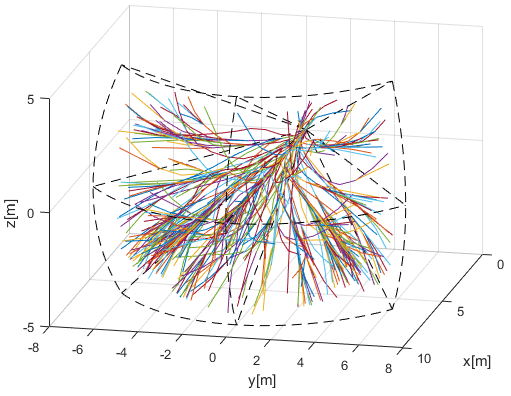
\includegraphics[width=0.7\textwidth]{\FIGDIR/P05ChaoticReachSetMethod}
    \caption{Trajectories for chaotic reach set approximation method}
    \label{fig:P05ChaoticReachSetMethod}
\end{figure}
The \emph{tuning parameter} $c$ is spread ratio, which defines how many nodes should be selected in each cell $c_{i,j,k}$. Example of reduced reach set approximating is given in fig. \ref{fig:P05ChaoticReachSetMethod}. \emph{Overall method performance} for various avoidance grid sizes:
\begin{enumerate}
    \item Don`t keep trajectories smoothness.
    \item Has high coverage. 
    \item Has high count of nodes.
\end{enumerate}

\subsection{Harmonic reach set approximation}\label{s:harmonicApproximationReachSet}
\noindent \emph{Main intention} is to create reduced reach set approximation $\mathscr{R}_R$. The \emph{smoothness} of generated trajectories is main priority. It is known that trajectory going trough cell center has higher probability to be smooth. The cost functional J (\ref{eq:harmonicExpansionCondition}) is product of smoothness function $P_S$ (\ref{eq:smmothnesFunction}) and inverted distance of last trajectory point $\mathscr{T}(\hat{x},B)\to\R^3$ to last passing cell center c.center. 

\begin{equation}\label{eq:harmonicExpansionCondition}
    J(\mathscr{N}(\textbf{x}),B,\mathscr{C}) =  \frac{1}{d(\text{c.center},\mathscr{T}(\hat{x},B)\to\R^3)}\times P_S(\mathscr{T}(\vec{x},B))
\end{equation}

\begin{figure}[H]
    \centering
    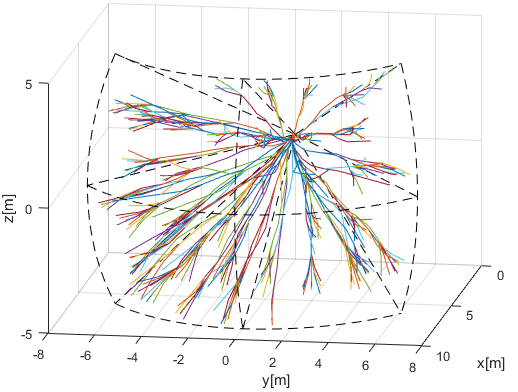
\includegraphics[width=0.7\textwidth]{\FIGDIR/P06HarmonicReachSetMethod}
    \caption{Trajectories for harmonic reach set approximation method}
    \label{fig:P06HarmonicReachSetMethod}
\end{figure}

\noindent \emph{Tuning parameter} $h$ decides how many nodes $\mathscr{N}$ in one cell $c_{i_{l_l},j,k}$ in layer $l_l\subset\mathscr{A}(t_i)$ will be expanded. The example of harmonic reach set is given in fig. \ref{fig:P06HarmonicReachSetMethod}. One can see that almost all trajectories have long straight (smooth) segments. Overall method performance for various avoidance grid sizes:
\begin{enumerate}
    \item Keep trajectories smoothness.
    \item Has low coverage.
    \item Has low count of nodes.
\end{enumerate}

\subsection{Combined reach set approximation}\label{s:combinedReachSetApproximation}
\noindent \emph{Chaotic reach set approximation} (sec. \ref{s:chaoticApproximationReachSet}) lacks smoothness of trajectories for navigation without obstacles, it has great coverage ration $C_R$. \emph{Harmonic reach set approximation} (sec. \ref{s:harmonicApproximationReachSet}) is great for navigation in unconstrained environment, but its coverage capabilities are low.

Because of existence of tuning parameters for \emph{chaotic reach set approximation} $c$ and \emph{harmonic reach set approximation} $h$ \emph{Combined method} can be proposed. Using following approach harmonic tree with expansion tuning parameters $h,c$ can be achieved:
\begin{enumerate}
    \item Create identical root nodes $\mathscr{N}_h(\textbf{x}=\hat{x}(t_i),B=\varnothing,J=0,\mathscr{C}=\varnothing)$ for harmonic expansion and $\mathscr{N}_c(\textbf{x}=\hat{x}(t_i),B=\varnothing,J=0,\mathscr{C}=\varnothing)$ for chaotic expansion.
    \item Expand harmonic root $\mathscr{N}_h$ using maximum criterion $J$ (\ref{eq:harmonicExpansionCondition}) and tuning parameter $h$.
    \item Expand chaotic root $\mathscr{N}_c$ using maximum criterion $J$ (\ref{eq:chaoticExpansionCondition}) and tuning parameter $c$.
    \item Merge chaotic tree with root $\mathscr{N}_c$  and harmonic tree with  root $\mathscr{N}_h$. Merge is possible because both tree structures are compatible and using same structures except expansion criterion (proof omitted). Example of merging multiple trees can be found in \cite{o1996log}.
\end{enumerate}

\begin{figure}[H]
    \centering
    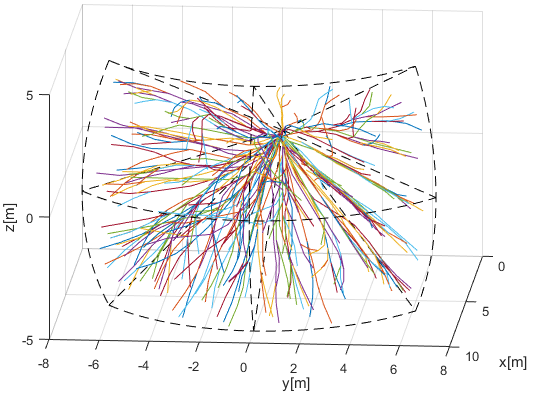
\includegraphics[width=0.7\textwidth]{\FIGDIR/P07CombinedReachSetMethod}
    \caption{Trajectories for combined reach set approximation method}
    \label{fig:P07CombinedReachSetMethod}
\end{figure}

\noindent Example of \emph{harmonic reach set approximation} is protrayed in fig. \ref{fig:P07CombinedReachSetMethod}. Overall method performance for various avoidance grid sizes:
\begin{enumerate}
    \item Keep trajectories smoothness.
    \item Has high coverage.
    \item Has medium count of nodes.
\end{enumerate}








\chapter{Probabilistic calculations}

\section{Intruder intersection model}\label{sec:intruderIntersectionModel}
\noindent \paragraph{Intruder model} is basically about intersection of 3D objects, because of definition of avoidance grid $\mathscr{A}(t_i)$ most of these methods are numeric. Let us introduce intruder model $\dot{\vec{x}}_I=\vec{f}(\vec{x}_I,\vec{u}_I)$ is given by following equation:
\begin{equation}\label{eq:intruderBasicLinearModel}
    \dot{\vec{x}}_I=
    \begin{aligned}
        \dot{p}_x\\
        \dot{p}_y\\
        \dot{p}_z
    \end{aligned}
    = 
    \begin{aligned}
        =v_x\\
        =v_y\\
        =v_z
    \end{aligned}
    ;\quad
    \vec{x}_I(0)=
    \begin{bmatrix}
        p_x(0)\\
        p_y(0)\\
        p_z(0)
    \end{bmatrix}
    ;\quad
    \begin{aligned}
        p_x(t)\\
        p_y(t)\\
        p_z(t)
    \end{aligned}
    \begin{aligned}
        =p_x(0)+v_x.t\\
        =p_y(0)+v_y.t\\
        =p_z(0)+v_z.t
    \end{aligned}
\end{equation}

\noindent Position vector $[p_x,p_y,p_z]^T$  $(m,m,m\in\R^3$ is given in local coordinate frame of avoidance grid $\mathscr{A}(t_i)$. Velocity vector $[v_x,v_y,v_z]$ $(m.s^{-1},m.s^{-1},m.s^{-1})$ is \emph{estimated and not changing}. The time $t$ is in interval $[t_e,t_l]$, where $t_e$ is intruder entry time into avoidance zone and $t_l$ is intruder leave time from avoidance zone, if vehicle is considered, time of entry is marked as $i_{e,k}$ where k is intruder identification, time of leave is marked as $i_{l,k}$ where k is intruder identification. 

\paragraph{Cell entry and leave times} $t_e(c_{i,j,k})$ and $t_l(c_{i,j,k})$ are given by trajectory $\mathscr{T}(x_0,B)$ and cell space $c_{i,j,k}\in\{x\in\R^3:d_s \le x(1) \le d_e, \theta_s \le x(2) \le \theta_e, \varphi_s \le x(3) \le \varphi_e \}$. From trajectory definition there exist projection $f:\mathscr{T}(x_0,B)\to (\R^3)\times \R$ to avoidance grid coordinate space $x\in \R^3$ and avoidance grid time $t\in\R$. Then intersection of trajectory and cell with time is given as:
\begin{equation}
    (\mathscr{T}(x_0,B)\to (\R^3)\times \R)\cap(c_{i,jk}\times (-\infty,\infty))=\left\{ \vec{x}_e,\dots,\vec{x}_l \right\}\times \left\{ t_e,...,t_l\right\}
\end{equation}
\noindent Where $t_e$ is cell $c_{i,j,k}$ entry time given by function $f_{t_e}(c_{i,j,k},\mathscr{T}(x_0,B))$, $t_l$ is cell leave time given by function $f_{t_l}(c_{i,j,k},\mathscr{T}(x_0,B))$. Entry time $t_e$ and leave time $t_l$ for cell $c_{i,j,k}$ where $\mathscr{T}(c_{i,j,k})$ is set of trajectories are given by eq. (\ref{eq:cellEntryTime}) and (\ref{eq:cellLeaveTime}).
\begin{equation}\label{eq:cellEntryTime}
    t_e=f_{t_e}(c_{i,j,k})=
    \begin{cases}
        -\infty&:|\mathscr{T}(c_{i,j,k})|=0\\
        \min f_{t_e}(c_{i,j,k},\mathscr{T}(x_0,B)),\forall\mathscr{T}(x_0,B)\in \mathscr{T}(c_{i,j,k})&:|\mathscr{T}(c_{i,j,k})|\neq 0\\
    \end{cases}
\end{equation}

\begin{equation}\label{eq:cellLeaveTime}
    t_l=f_{t_l}(c_{i,j,k})=
    \begin{cases}
        \infty&:|\mathscr{T}(c_{i,j,k})|=0\\
        \max f_{t_l}(c_{i,j,k},\mathscr{T}(x_0,B)),\forall\mathscr{T}(x_0,B)\in \mathscr{T}(c_{i,j,k})&:|\mathscr{T}(c_{i,j,k})|\neq 0\\
    \end{cases}
\end{equation}

\paragraph{Intruder intersection probability} $P_{O_I}(i_k)$ for intruder $i_k$ intersection with vehicle in cell $c_{i,j,k}$ is given by eq. (\ref{eq:intruderIntersectionProbability}).
\begin{equation}\label{eq:intruderIntersectionProbability}
    P_{O_I}(i_k)=\frac{\norm{[i_e(c_{i,j,k}),i_l(c_{i,j,k})]\cap [t_e,t_l]}}{\norm{[t_e,t_l]}}.P_T(i_k,c_{i,j,k})
\end{equation}
\noindent Base intersection probability $P_T(i_k,c_{i,j,k})$ shows how probable is to meet intruder $i_k$ in cell $c_{i,j,k}$, enumerator $\norm{[i_e(c_{i,j,k}),i_l(c_{i,j,k})]\cap [t_e,t_l]}$ represents time duration which intruder $i_k$ and our vehicle spends together in cell $c_{i,jk}$, where $i_e$ is intruder entry, $i_l$ is intruder leave, $t_e$ is vehicle entry, $t_l$ is vehicle leave, denominator $\norm{[t_e,t_l]}$ is maximum duration of vehicle passing trough cell $c_{i,j,k}$. \textit{The main principle} is to calculate probability of staying in same portion of space for vehicle and intruder $i_k$. In case the numeric approximation is used and the result is set of intersection times/position pairs $\{(t_1,\vec{p}_1),\dots,(t_k,\vec{p}_k)\}$ where position set $\{\vec{p}_1,\dots,\vec{p}_k\}\in c_{i,j,k}$  then (\ref{eq:intruderIntersectionProbability}) is re-written as:
\begin{equation}\label{eq:intruderIntersectionProbabilityNumeric}
    P_{O_I}(i_k)=\frac{|\{t_1,\dots,t_k\}\cap [t_e,t_l]|}{k}.P_T(i_k,c_{i,j,k}),\quad \{t_1,\dots,t_k\},k\in \N^+
\end{equation}
\noindent Base intersection probability $P_T(i_k,c_{i,j,k})$  stays same it is not impacted. The time intersection probability is calculated differently, enumerator  $|\{t_1,\dots,t_k\}\cap [t_e,t_l]|$ is resulting into count of how many numeric hits landed vehicle entry/leave interval $[t_e,t_l]$. Denominator is simple count of hits which landed into cell $c_i,j,k$. The final ratio shows how probable is to encounter intruder $i_k$ in cell $c_{i,j,k}$. The principle of (\ref{eq:intruderIntersectionProbabilityNumeric}) is same as (\ref{eq:intruderIntersectionProbability})  but instead of interval intersection, set intersection is used.

\paragraph{Base intersection probability} $P_T(i_k,c_{i,j,k})$ reflects probability of vehicle intersection with portion of space occupied by cell $c_{i,j,k}$, to be precise with vehicle trajectory or vehicle body shifted among that trajectory. This work considers two trajectories representation:
\begin{enumerate}
    \item \textit{Direct line} - vehicle trajectory is represented as basic linear model (\ref{eq:intruderBasicLinearModel}), depending on average cell volume and safety margin condition direct line can have two intersection modes:
    \begin{enumerate}[a.]
        \item \textit{simple line} - intersection is approximated along line defined by intruder model (\ref{eq:intruderBasicLinearModel}).
        \item \textit{volume line} - intersection is approximated along line defined by intruder model (\ref{eq:intruderBasicLinearModel}) and intruder radius $r_i$ $[m]$ is considered in intersection.
    \end{enumerate}
    \item \textit{Elliptic cone} - initial position $\vec{x}_i(0)$ is considered as top of the cone, main cone axis is given by line (\ref{eq:intruderBasicLinearModel}) $t\in [-\infty,\infty]$. The cone is defined by horizontal spread parameter $\theta$ and vertical spread $\varphi$.
\end{enumerate}

\paragraph{Base intersection probability - simple line type} $P_T(i_k(\vec{x},\vec{v}),c_{i,j,k})$ is simple linear intersection with line defined as expected intruder $i_r$ trajectory (\ref{eq:linearModelIntruderLineIntersection}). Intruder trajectory is defined by starting point $\vec{x}_s\in\R^3$ and linear velocity vector $\vec{v}\in\R^3$. 
\begin{equation}\label{eq:linearModelIntruderLineIntersection}
    \vec{x}(t)=\vec{x}_s + \vec{v}_I.t
\end{equation}
\noindent Then there exist projection function from local euclidean coordinates to local planar coordinates $p(t)$ (\ref{eq:projecionFunctionplanarEuclidlinearIntersection}). Which projects trajectory of the system $\vec{x}(t)\in\R^3$ to planar coordinates $[d(t),\theta(t),\varphi(t)]$. Where $d$ is distance, $\theta$ is horizontal offset angle from main axis, and $\varphi$ is vertical offset angle from main axis.
\begin{equation}\label{eq:projecionFunctionplanarEuclidlinearIntersection}
    \vec{p}(t):\vec{x}(t)\to[d(t),\theta(t),\varphi(t)]
\end{equation}
\noindent The \emph{base intersection probability} $P_T(i_k(\vec{x},\vec{v}),c_{i,j,k})$ for line type is given as eq. \ref{eq:baseIntersectionProbabilityLineIntersectionType}. If there exist non empty intersection of $p(t)\cap c_{i,j,k}$ there is direct collision probability, if intersection $p(t)\cap c_{i,j,k} = \varnothing$ then probability is zero.
\begin{equation}\label{eq:baseIntersectionProbabilityLineIntersectionType}
    P_T(i_k(\vec{x},\vec{v}),c_{i,j,k})=
    \begin{cases}
        1&\exists d(t),\theta(t),\varphi(t),[d(t),\theta(t),\varphi(t)]^T\in c_{i,j,k}\\
        0&\text{otherwise}
    \end{cases}
\end{equation}

\paragraph{Base intersection probability - volume line type} $P_T(i_k(\vec{x},\vec{v},r),c_{i,j,k})$ is defined for linear intersection model $\vec{x}(t)$ (\ref{eq:linearintersectionmodelVehicleVolume}) where initial position $\vec{x}_s$ is given at expected time of avoidance $t_i$ in avoidance grid $\mathscr{A}(t_i)$ local coordinate frame, velocity vector $\vec{v}$ is given in same reference frame.
\begin{equation}\label{eq:linearintersectionmodelVehicleVolume}
    \vec{x}(t)=\vec{x}_s + \vec{v}.t
\end{equation}

\noindent\emph{Volume ball} $\mathscr{B}(\vec{x}(t),r)$ (\ref{eq:volumeballofIntruder}) is defined as set of points in $\R^3$ space with defined center at intruder $i_r$ position $\vec{x}(t)$. The inclusion criterion is set to a full ball. Volume ball $\mathscr{B}(\vec{x}(t),r)$ represents approximation of vehicle body expected position at time $t$.
\begin{equation}\label{eq:volumeballofIntruder}
    \mathscr{B}(\vec{x}(t),r)= \left\{\vec{a}\in\R^3:\exists t,\norm{\vec{a}-\vec{x}(t)}_2\le r\right\}
\end{equation}

\noindent\emph{Planar volume ball} $\mathscr{P}_\mathscr{B}$ (\ref{eq:plannarCoordinateTransformationVolumeBall}) is projection of volume ball $\mathscr{B}(\vec{x}(t))$ to a set of planar coordinates $\left\{[d,\theta,\varphi]\right\}$ in avoidance grid $\mathscr{A}(t_i)$ local coordinate frame for expected avoidance time $t_i$.
\begin{equation}\label{eq:plannarCoordinateTransformationVolumeBall}
    \mathscr{P}_\mathscr{B}=\mathscr{B}(\vec{x}(t),r)\to \left\{[d,\theta,\varphi]\right\}
\end{equation}

\noindent\emph{Base intersection probability for vehicle body} $P_T(i_k(\vec{x},\vec{v},r),c_{i,j,k})$ \ref{eq:baseIntersectionProbabilityBallIntersectionType} is calculated as intersection of planar volume ball $\mathscr{P}_\mathscr{B}$ and cell $c_{i,j,k}$. If intersection $\mathscr{P}_\mathscr{B}\cap c_{i,j,k} \neq \varnothing$ is non empty then base probability is one, zero otherwise.
\begin{equation}\label{eq:baseIntersectionProbabilityBallIntersectionType}
    P_T(i_k(\vec{x},\vec{v},r),c_{i,j,k})=
    \begin{cases}
        1&\mathscr{P}_\mathscr{B}\cap c_{i,j,k} \neq \varnothing\\
        0&\text{otherwise}
    \end{cases}
\end{equation}

\paragraph{Base intersection probability - elliptic cone type} $P_T(i_k(\vec{x}_s,\vec{v},\theta,\varphi),c_{i,j,k})$
computation is less straight-forward than other base intersection probabilities. First let us define linear intruder $i_k$ positions $\vec{x}$ at time $t$ (\ref{eq:vehiclelinearcone}) model, where $\vec{x}(t)$ defines vehicle position in \emph{vehicle local coordinate frame} at time of avoidance, $\vec{v}$ defines intruder velocity, and $t$ is time offset.
\begin{equation}\label{eq:vehiclelinearcone}
    \vec{x}(t)=\vec{x}_s + \vec{v}_I.t
\end{equation}
\noindent Intruder \emph{horizontal spread} $\theta$ and \emph{vertical spread} $\varphi$ are introduced. These spreads represents intruder deviation limits from original trajectory $\vec{x}(t)\in\R^3$. The example is given by fig. \ref{fig:P21ElipticConeIOnePoint} where intruder starts at point $\vec{x}_s$ with some velocity $v$, the linear trajectory approximation is given by blue line. \emph{Intruder position} at time $t=10s$ is given by $\vec{x}(10)$ and is denoted blue point. The ellipsoidal space $E(\vec{x})$ is projected on plane $D(\vec{x}(t))$. The plane $D$ (\ref{eq:elisioidalOtrthogonalPlane}) for point $\vec{x}(t)$ and velocity $\vec{v}$ is defined as orthogonal plane to velocity $\vec{v}\in\R^3$ with origin at intruder position $\vec{x}(t)$. 
\begin{equation}\label{eq:elisioidalOtrthogonalPlane}
    D(\vec{x}(t),\vec{v})=\left\{\vec{a}\in\R^3:(\vec{a}-\vec{x}(t))\perp\vec{v},\right\}
\end{equation}
\noindent To introduce ellipsoidal space on orthogonal plane $D(\vec{x}(t),\vec{v})$ some parameters are introduced in eq. (\ref{eq:elipsiodialBoudaryParameters}). The \emph{scalar distance} $d_d{\vec{x}(t)}$ is simple euclidean norm, \emph{maximal horizontal offset} $d_\theta(\vec{x}_t)$ is given as product of sinus of horizontal offset angle $\theta$ and scalar distance $d_d$, and \emph{maximal vertical offset} $d_\varphi(\vec{x}(t))$ is given a product of sinus of vertical offset angle $\varphi$ and scalar distance $d_d$.
\begin{equation}\label{eq:elipsiodialBoudaryParameters}
    \begin{aligned}
     d_d                      &=d_d(\vec{x}(t),\vec{x}_s) =\norm{\vec{x}(t)-\vec{x}_s}_2\\ 
     d_{\theta_{\text{max}}}  &= d_\theta(\vec{x}(t))=\sin\theta   (i_k).d_d(\vec{x}(t))\\
     d_{\varphi_{\text{max}}} &= d_\varphi(\vec{x}(t))=\sin\varphi (i_k).d_d(\vec{x}(t)) 
    \end{aligned}
\end{equation}
\begin{figure}[H]
    \centering
    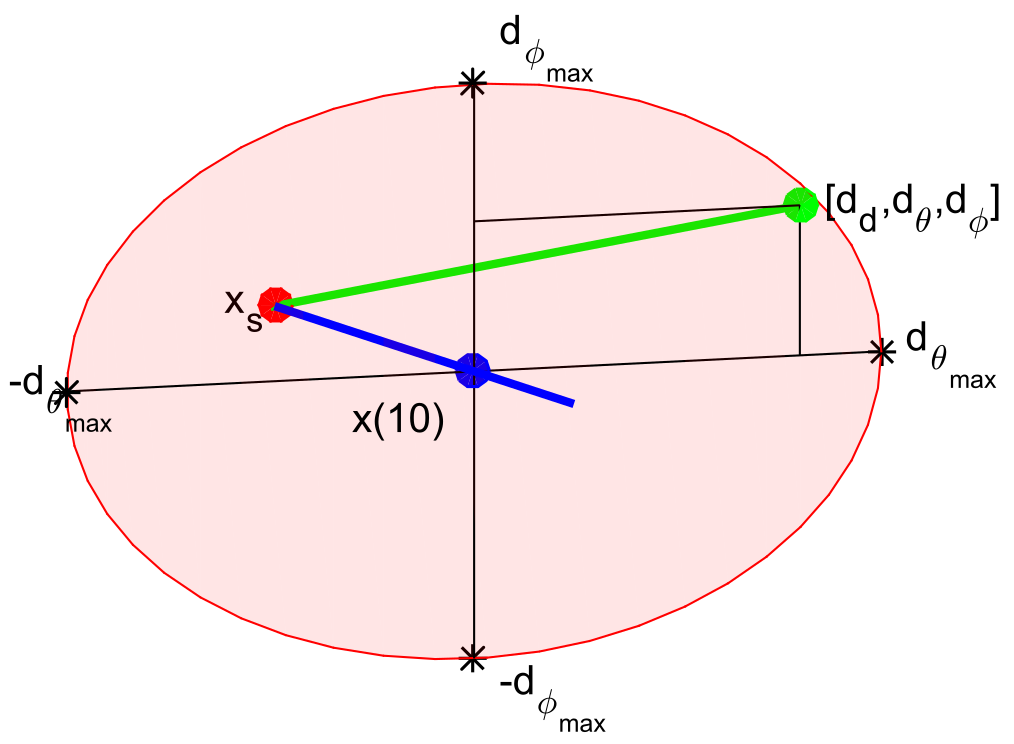
\includegraphics[width=0.7\textwidth]{\FIGDIR/P21ElipticConeIOnePoint}
    \caption{One probable position $[d_d,d_\theta,d_\varphi]$ (green). deviated from linear trajectory (blue line) at point $\vec{x}(10)$.(blue) with initial position $x_s$ (red)}
    \label{fig:P21ElipticConeIOnePoint}
\end{figure}
\noindent \emph{Ellipsoid} $E(\vec{x}(t),\vec{v})$ (\ref{eq:baseElipsoidxt}) for some intruder position $\vec{x}(t)$ and intruder velocity $\vec{v}$ is given as constrained subspace of orthogonal plane $D(\vec{x}(t),\vec{v})$. The constraint is defined by internal coordinate frame $\vec{p}\in \R^2$ which is space reduction of plane $D(\vec{x}(t),\vec{v})$. Internal coordinate frame $\vec{p}\in\R^2$ has origin in $\vec{x}(t)\to\R^2$. The points of plane $\vec{p}$ are bounded by projection $\vec{p}=(\vec{b}-\vec{x}(t))\to\R^2$, where $b\in D(\vec{x}(t),v)$. The point of ellipsoidal $\vec{p}$ is then given as standard ellipse boundary with vertical span $d_\theta(\vec{x}(t))$ and horizontal span $d_\varphi(\vec{x}(t))$. \emph{Ellipsoid} $E(\vec{x}(t),\vec{v})$ for specific time $t=10s$ example is portrayed  as red elipsoind in fig. \ref{fig:P21ElipticConeIOnePoint}.
\begin{equation}\label{eq:baseElipsoidxt}
    E(\vec{x}(t),\vec{v})=\left\{ \begin{aligned}\vec{b}\in\R^3:&\vec{b}\in D(\vec{x}(t),\vec{v}),\vec{p}=(\vec{b}-\vec{x}(t))\to\R^2,\\&\left(\frac{p(1)^2} {d_\theta(\vec{x}(t))^2}+ \frac{p(2)^2}{d_\varphi(\vec{x}(t))^2}\right)\le 1\end{aligned}\right\}
\end{equation}

\noindent The expected behaviour of intruder $i_k$ is to stick to linear trajectory $\vec{x}(t)$ (\ref{eq:vehiclelinearcone}). The probability of deviation should be decreasing with distance from ellipse center (fig. \ref{fig:P22ProbabilisticDistributionOfEllipsoidCut}.).  
\begin{figure}[H]
    \centering
    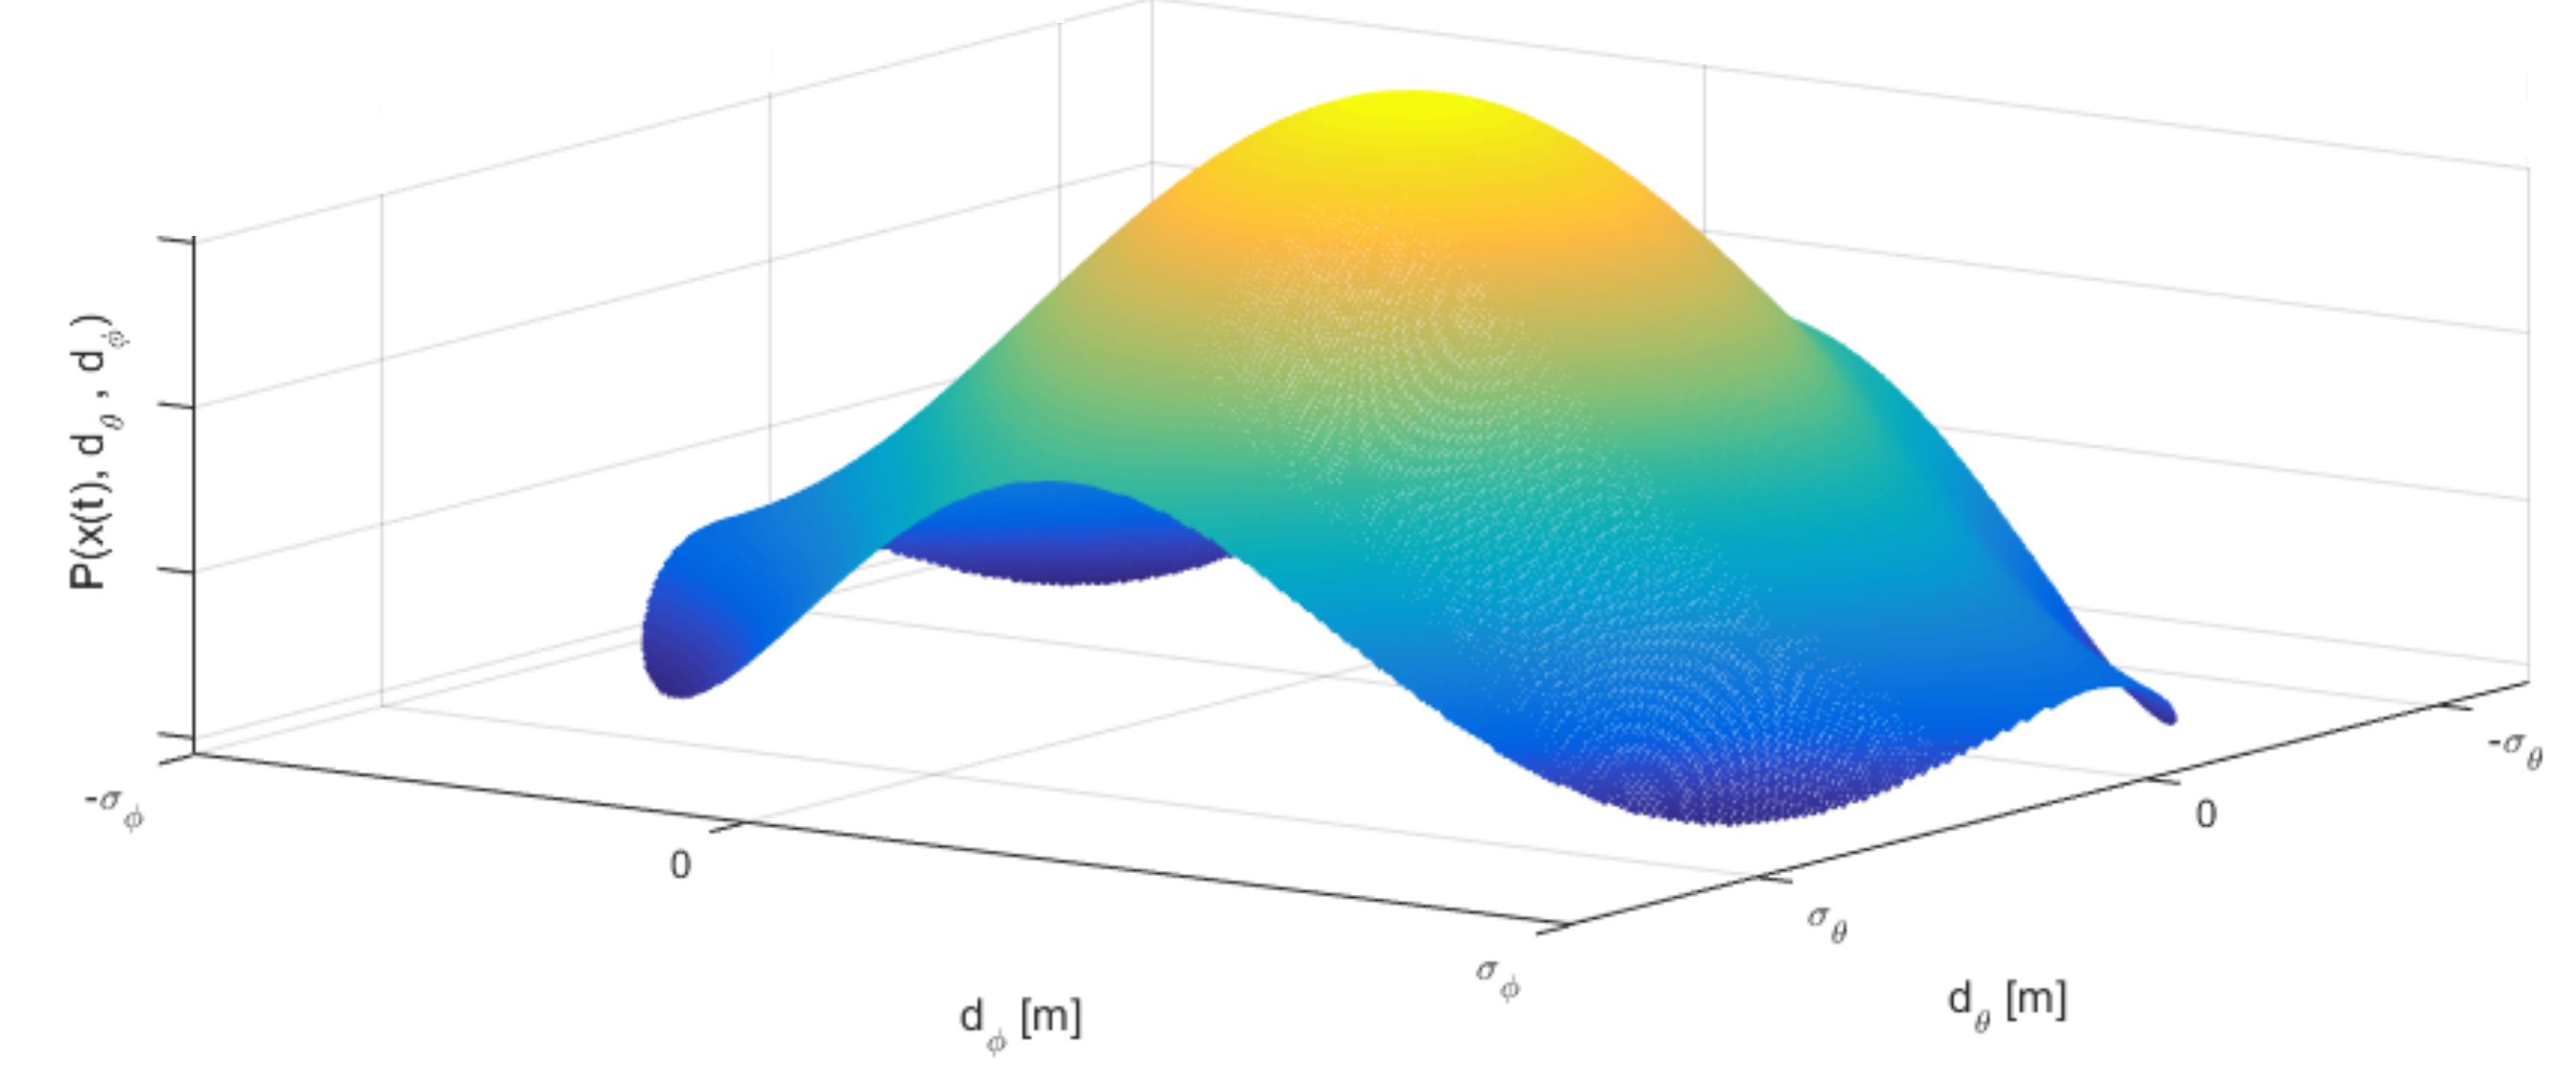
\includegraphics[width=0.9\textwidth]{\FIGDIR/P22ProbabilisticDistributionOfEllipsoidCut}
    \caption{Probability of intruder $i_k$ position in ellipsoid $E(\vec{x}(t),\vec{v})$}
    \label{fig:P22ProbabilisticDistributionOfEllipsoidCut}
\end{figure}
\noindent \emph{Probability density function} for ellipsoid  $E(\vec{x}(t),\vec{v})$defined in (\ref{eq:baseElipsoidxt}) is depending on maximal horizontal spread $d_\theta(\vec{x}(t))$, maximal vertical spread $d_\varphi(\vec{x}(t))$, defined by eq. \ref{eq:elipsiodialBoudaryParameters}. Two standard probabilistic distributions are established $\mathscr{N}(\mu_\theta,\sigma_\theta)$ (\ref{eq:elipsprobdistHorizontal}) for horizontal spread $\theta(\vec{x}(t))$ and $\mathscr{N}(\mu_\varphi,\sigma_\varphi)$  (\ref{eq:elipsprobdistVertical}) for vertical spread $\varphi(\vec{x}(t))$. The means $\mu_\theta$ and $\mu_\varphi$ are set to zero, and internal coordinate frame $\vec{p}\in\R^2$ where $\vec{x}(t)\to\R^2$ is frame center. The variances $\sigma_\theta$ and $\sigma_\varphi$ are set as maximal distances on horizontal/vertical spread axes $d_\theta(\vec{x}(t))$ and $d_\varphi(\vec{x}(t))$.
\begin{equation}\label{eq:elipsprobdistHorizontal}
    P(\vec{x}(t),d_\theta)=\mathscr{N}(\mu_\theta,\sigma_\theta)=\mathscr{N}(0,d_\theta(\vec{x}(t)))
\end{equation}
\begin{equation}\label{eq:elipsprobdistVertical}
    P(\vec{x}(t),d_\varphi)=\mathscr{N}(\mu_\varphi,\sigma_\varphi)=\mathscr{N}(0,d_\varphi(\vec{x}(t)))
\end{equation}
\noindent Combined \emph{probability density function} for maximal spreads $d_\theta$ and $d_\varphi$ is given by eq. \ref{eq:elipsprobdistCombined}. Because probability density function is defined for internal space $\vec{p}\in\R^2$ and one may need to calculate probability for for cell space $c_{i,j,k}\in\R^3$, the reduction from two parameter probability distribution function to scalar probability distribution function is needed. Scalar probabilistic distribution  function $P(\vec{x}(t),d_\theta,d_\varphi)$ over ellipsoid $E(\vec{x}(t),\vec{v})$ is introduced (\ref{eq:elipsprobdistCombined}), where final probability is given as average of two partial probabilities. Final $P(\vec{x}(t),d_\theta,d_\varphi)$ needs to be normalized to hold \emph{normal distribution condition} (\ref{eq:normalDistrobitionCondition}). Normal distribution condition value (\ref{eq:normalDistrobitionCondition}) is given as surface integral over ellipsoid $E(\vec{x}(0),\vec{v})$ with probability density function $P(\vec{x}(t),d_\theta,d_\varphi)$.
\begin{equation}\label{eq:elipsprobdistCombined}
    P(\vec{x}(t),d_\theta,d_\varphi) = \frac{\mathscr{N}(\mu_\theta,\sigma_\theta)+\mathscr{N}(\mu_\varphi,\sigma_\varphi)}{2}
\end{equation}
\begin{equation}\label{eq:normalDistrobitionCondition}
    \iint_{E(\vec{x}(\tau))} P(\vec{x}(t),d_\theta,d_\varphi) \,\text{d}d_\theta\,\text{d}d_\varphi = 1
\end{equation}
\noindent Final intersection probability  $P(\vec{x}(t),c_{i,j,k},\theta,\varphi)$ (static part, timed is calculated in (\ref{eq:intruderIntersectionProbability}) is given by eq. \ref{eq:spreadIntruderIntersectionProb}. Its mean value of all intersection probabilities $P(\vec{x}(\tau),c_{i,j,k},\theta,\varphi)$ where $\tau\in[i_e(c_{i,j,k}),i_l(c_{i,j,k})]$ is fixed point in intersection time interval. $P(\vec{x}(\tau),c_{i,j,k},\theta,\varphi)$ (\ref{eq:spreadIntersectionProbFixedtau}) is integration of probability density function $P(\vec{x}(\tau),d_\theta,d_\varphi)$ (\ref{eq:elipsprobdistCombined}) in surface $E(\vec{x}(\tau),\vec{v})$ to cell $c_{i,j,k}$ volume intersection. To get volume integration partial probability in surface intersection must be integrated and normalized in time interval $\tau\in[i_e(c_{i,j,k}),i_l(c_{i,j,k})]$, the \emph{base intersection probability} $P_T(i_k(\vec{x}_s,\vec{v},\theta,\varphi),c_{i,j,k})$ is given by eq. \ref{eq:spreadIntruderIntersectionProb}. Example of intersection of intruder $i_r$ uncertain ellipsoid cone with avoidance grid $\mathscr{A}(t_i)$ is given in fig. \ref{fig:P20ElipticConeIntersecitonExample}.
\begin{equation}\label{eq:spreadIntersectionProbFixedtau}
    P(\vec{x}(\tau),c_{i,j,k},\theta,\varphi) =\iint_{E(\vec{x}(\tau),\vec{v})\cap c_{i,j,k}} P(\vec{x}(\tau),d_\theta,d_\varphi)
\end{equation}
\begin{equation}\label{eq:spreadIntruderIntersectionProb}
    P_T(i_k(\vec{x}_s,\vec{v},\theta,\varphi),c_{i,j,k})=\frac{\int_{i_e(c_{i,j,k})}^{i_l(c_{i,j,k})} P(\vec{x}(\tau),c_{i,j,k},\theta,\varphi)\,\text{d}\tau}{i_l(c_{i,j,k})-i_e(c_{i,j,k})}
\end{equation}
\begin{figure}[H]
    \centering
    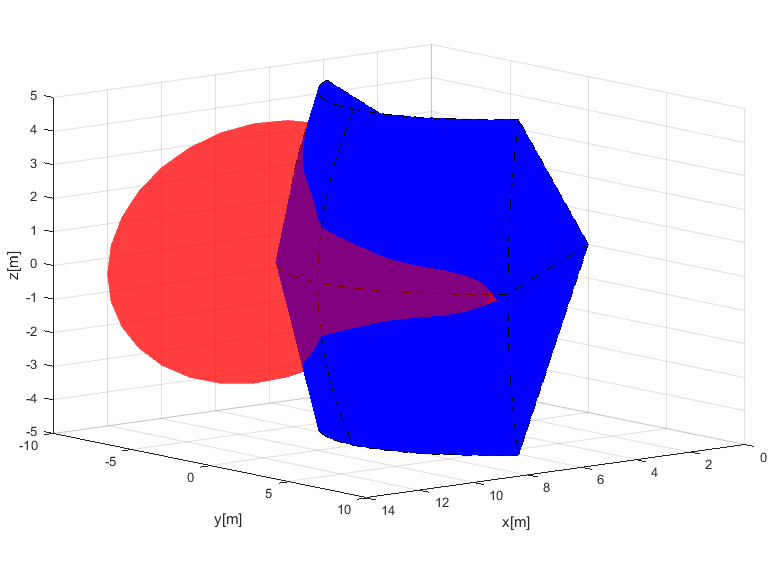
\includegraphics[width=0.7\textwidth]{\FIGDIR/P20ElipticConeIntersecitonExample}
    \caption{Avoidance grid $\mathscr{A}(t_i)$ (blue) intersection with elliptic cone intruder $i_k(\vec{x},\vec{v},\theta,\varphi)$ (red) example.}
    \label{fig:P20ElipticConeIntersecitonExample}
\end{figure}
\noindent \emph{Numeric approximation} of $P_T(i_k(\vec{x}_s,\vec{v},\theta,\varphi),c_{i,j,k})$ is more feasible than symbolic calculation due the multiple intersection constraints and bad intersection algorithm complexity. Let us define homogeneous discrete subset of real numbers $\mathscr{R}$ which is non empty subset of real numbers $\R$. The set $\mathscr{R}$ (\ref{eq:homogeneusdiscretizationofRealnumbers}) is homogeneous, that means for any equal interval $(i,i+1],i\in\mathbb{Z}$ subset the count of members is equal to some positive natural number $k$. The parameter $k$ can be understand as \emph{unit approximation density}.
Similarly the power sets $\mathscr{R}^2\subset\R^2$, $\mathscr{R}^3\subset\R^3$, ... $\mathscr{R}^i\subset\R^i,i\in\N^+$ keeps homogeneous distribution.
\begin{equation}\label{eq:homogeneusdiscretizationofRealnumbers}
    \mathscr{R} = \left\{\begin{aligned}a\in\R:&\forall i\in\mathbb{Z},|i<a\le i+1|=k,k\in\N^+, \\&\forall j\in \N^+a_{j+1}-a_{j}=m,m\in\R^+\end{aligned}\right\},\,\mathscr{R}\subset\mathbb{R}
\end{equation}
\noindent Orthogonal plane for $\vec{x}(t), \vec{v}, t \in\R$ is defined by eq. \ref{eq:elisioidalOtrthogonalPlane}. The orthogonality property is also kept for any subspace $\mathscr{R}^n\in\R^n,n\in\N^+$. Numeric approximation of $D(\vec{x}(t),\vec{v})$ is given as $D_D(\vec{x}(t),\vec{v})$ (\ref{eq:elisioidalOtrthogonalPlaneDiscrete}). The only difference is that discrete approximation is countable $|D_D|=m,m\in\N^+$, but continuous representation $|D|\approx \infty$ is uncountable. Because ellipsoid is subset of orthogonal plane it keep its countability property, therefore $E_D$ is also countable and must contains at-least one member.  
\begin{equation}\label{eq:elisioidalOtrthogonalPlaneDiscrete}
    D_D(\vec{x}(t),\vec{v})=\left\{\vec{a}\in\mathscr{R}^3:(\vec{a}-\vec{x}(t))\perp\vec{v},\right\},t\in\mathscr{R}
\end{equation}
\noindent\emph{Base ellipsoid} $E(\vec{x}(t),\vec{v})$ for continuous-space is given by eq. \ref{eq:baseElipsoidxt}. Every aspect, expect the base of internal projection $\mathscr{R}^2$ and orthogonal plane $D_D$ is same in discrete case $E_D(\vec{x}(t),\vec{v})$ (\ref{eq:baseElipsoidxtDiscrete}).
\begin{equation}\label{eq:baseElipsoidxtDiscrete}
    \bar{E}_D(\vec{x}(t),\vec{v})=\left\{ \begin{aligned}\vec{b}\in\mathscr{R}^3:&\vec{b}\in D_D(\vec{x}(t),\vec{v}),\vec{p}=(\vec{b}-\vec{x}(t))\to\mathscr{R}^2,\\&\left(\frac{p(1)^2} {d_\theta(\vec{x}(t))^2}+ \frac{p(2)^2}{d_\varphi(\vec{x}(t))^2}\right)\le 1\end{aligned}\right\},t\in\mathscr{R}
\end{equation}
\noindent \emph{Numeric disproportion} can occur in case that ellipsoid $\bar{E}_D(\vec{x}(t),\vec{v})$ (\ref{eq:baseElipsoidxtDiscrete}) in case of $d_\theta(\vec{x}(t))\approx 0$ and $d_\varphi(\vec{x}(t))\approx 0$. The count of elipsoid members can be $|\bar{E}_D(\vec{x}(t),\vec{v})|=0$, which is in contradiction with assumption $|\bar{E}_D(\vec{x}(t),\vec{v})|\neq 0$. Let assume for discrete times $\tau=\left\{t_1,t_2,\dots,t_i\right\}$, $i\in \N^+$ there exists ellipsoids $\bar{E}_D(\vec{x}(t_1),\vec{v})$,$\bar{E}_D(\vec{x}(t_1),\vec{v})$, $\dots$, $\bar{E}_D(\vec{x}(t_i),\vec{v})$ which are non empty and in space $\mathscr{R}^2$ in internal coordinate frame and space $\mathscr{R}^3$ in avoidance grid $\mathscr{A}(t_i)$ coordinate frame. The intersection of these partial ellipsoids in both spaces is equal to:
\begin{equation}
    \bar{E}_D(\vec{x}(t_1),\vec{v})\cap \bar{E}_D(\vec{x}(t_2),\vec{v})\dots\cap\dots \bar{E}_D(\vec{x}(t_i),\vec{v}) = \varnothing
\end{equation}
\noindent \emph{Empty intersection} enables us to keep homogeneity property of ellipsoids by adding points so it is safe to add specific point $\vec{x}(t)$ into empty ellipsoid. But only one, because it does not impact probability density functions $\mathscr{N}(\mu_\theta,\sigma_\theta)$ and $\mathscr{N}(\mu_\varphi,\sigma_\varphi)$, neither combined probability density function $P(\vec{x},d_\theta,d_\varphi)$. The final ellipsoid used forward $E_D(\vec{x}(t),\vec{v})$(\ref{eq:baseElipsoidxtDiscreteSafe}) is keeping all properties of ellipsoid $E(\vec{x}(t),\vec{v})$ (\ref{eq:baseElipsoidxtDiscreteSafe}). 
\begin{equation}\label{eq:baseElipsoidxtDiscreteSafe}
    E_D(\vec{x}(t),\vec{v})= 
    \begin{cases}
        |\bar{E}_D(\vec{x}(t),\vec{v})|=0 &: \left\{\vec{x}(t)\right\} \\
        |\bar{E}_D(\vec{x}(t),\vec{v})|\ge0 &: \bar{E}_D(\vec{x}(t),\vec{v}) 
    \end{cases}
\end{equation}
\noindent Normal distribution condition for probability function $P_D(\vec{x}(t),d_\theta,d_\varphi,\vec{p})$, which is instance of to probability density function $P(\vec{x}(y),d_\theta,d_\varphi)$ (\ref{eq:elipsprobdistCombined}) is used. This probabilistic distribution must be normalized according to eq.  \ref{eq:normalDistrobitionConditionDiscrete}. 
\begin{equation}\label{eq:normalDistrobitionConditionDiscrete}
    \sum_{\vec{p} \in E_D(\vec{x}(t))} P_D(\vec{x}(t),d_\theta,d_\varphi,\vec{p}) = 1,\forall t\in\mathscr{R}^+
\end{equation}
\noindent Equations for \emph{base intersection probability} are similar to eq. \ref{eq:spreadIntersectionProbFixedtau}, \ref{eq:spreadIntruderIntersectionProb}. For cell $c_{i,j,k}$ there exist intruder entry time $i_e(c_{i,j,k})$ its the earliest intersection with ellipsoid $E_D(\vec{x}(i_e(c_{i,j,k}))),\vec{v}$. Same situation occurs with intruder leave time $i_l(c_i,j,k)$. Because $E_D$ is countable set, it means additional attributes can be attached to each point $\vec{p}\in E_D$. Based on system dynamic (\ref{eq:intruderBasicLinearModel}) the \emph{Time Of Arrival} (TOA) can be calculated. The example of TOA is given in fig. \ref{fig:P23EllipsoidCutTimeOfArrival}.
\begin{figure}[H]
    \centering
    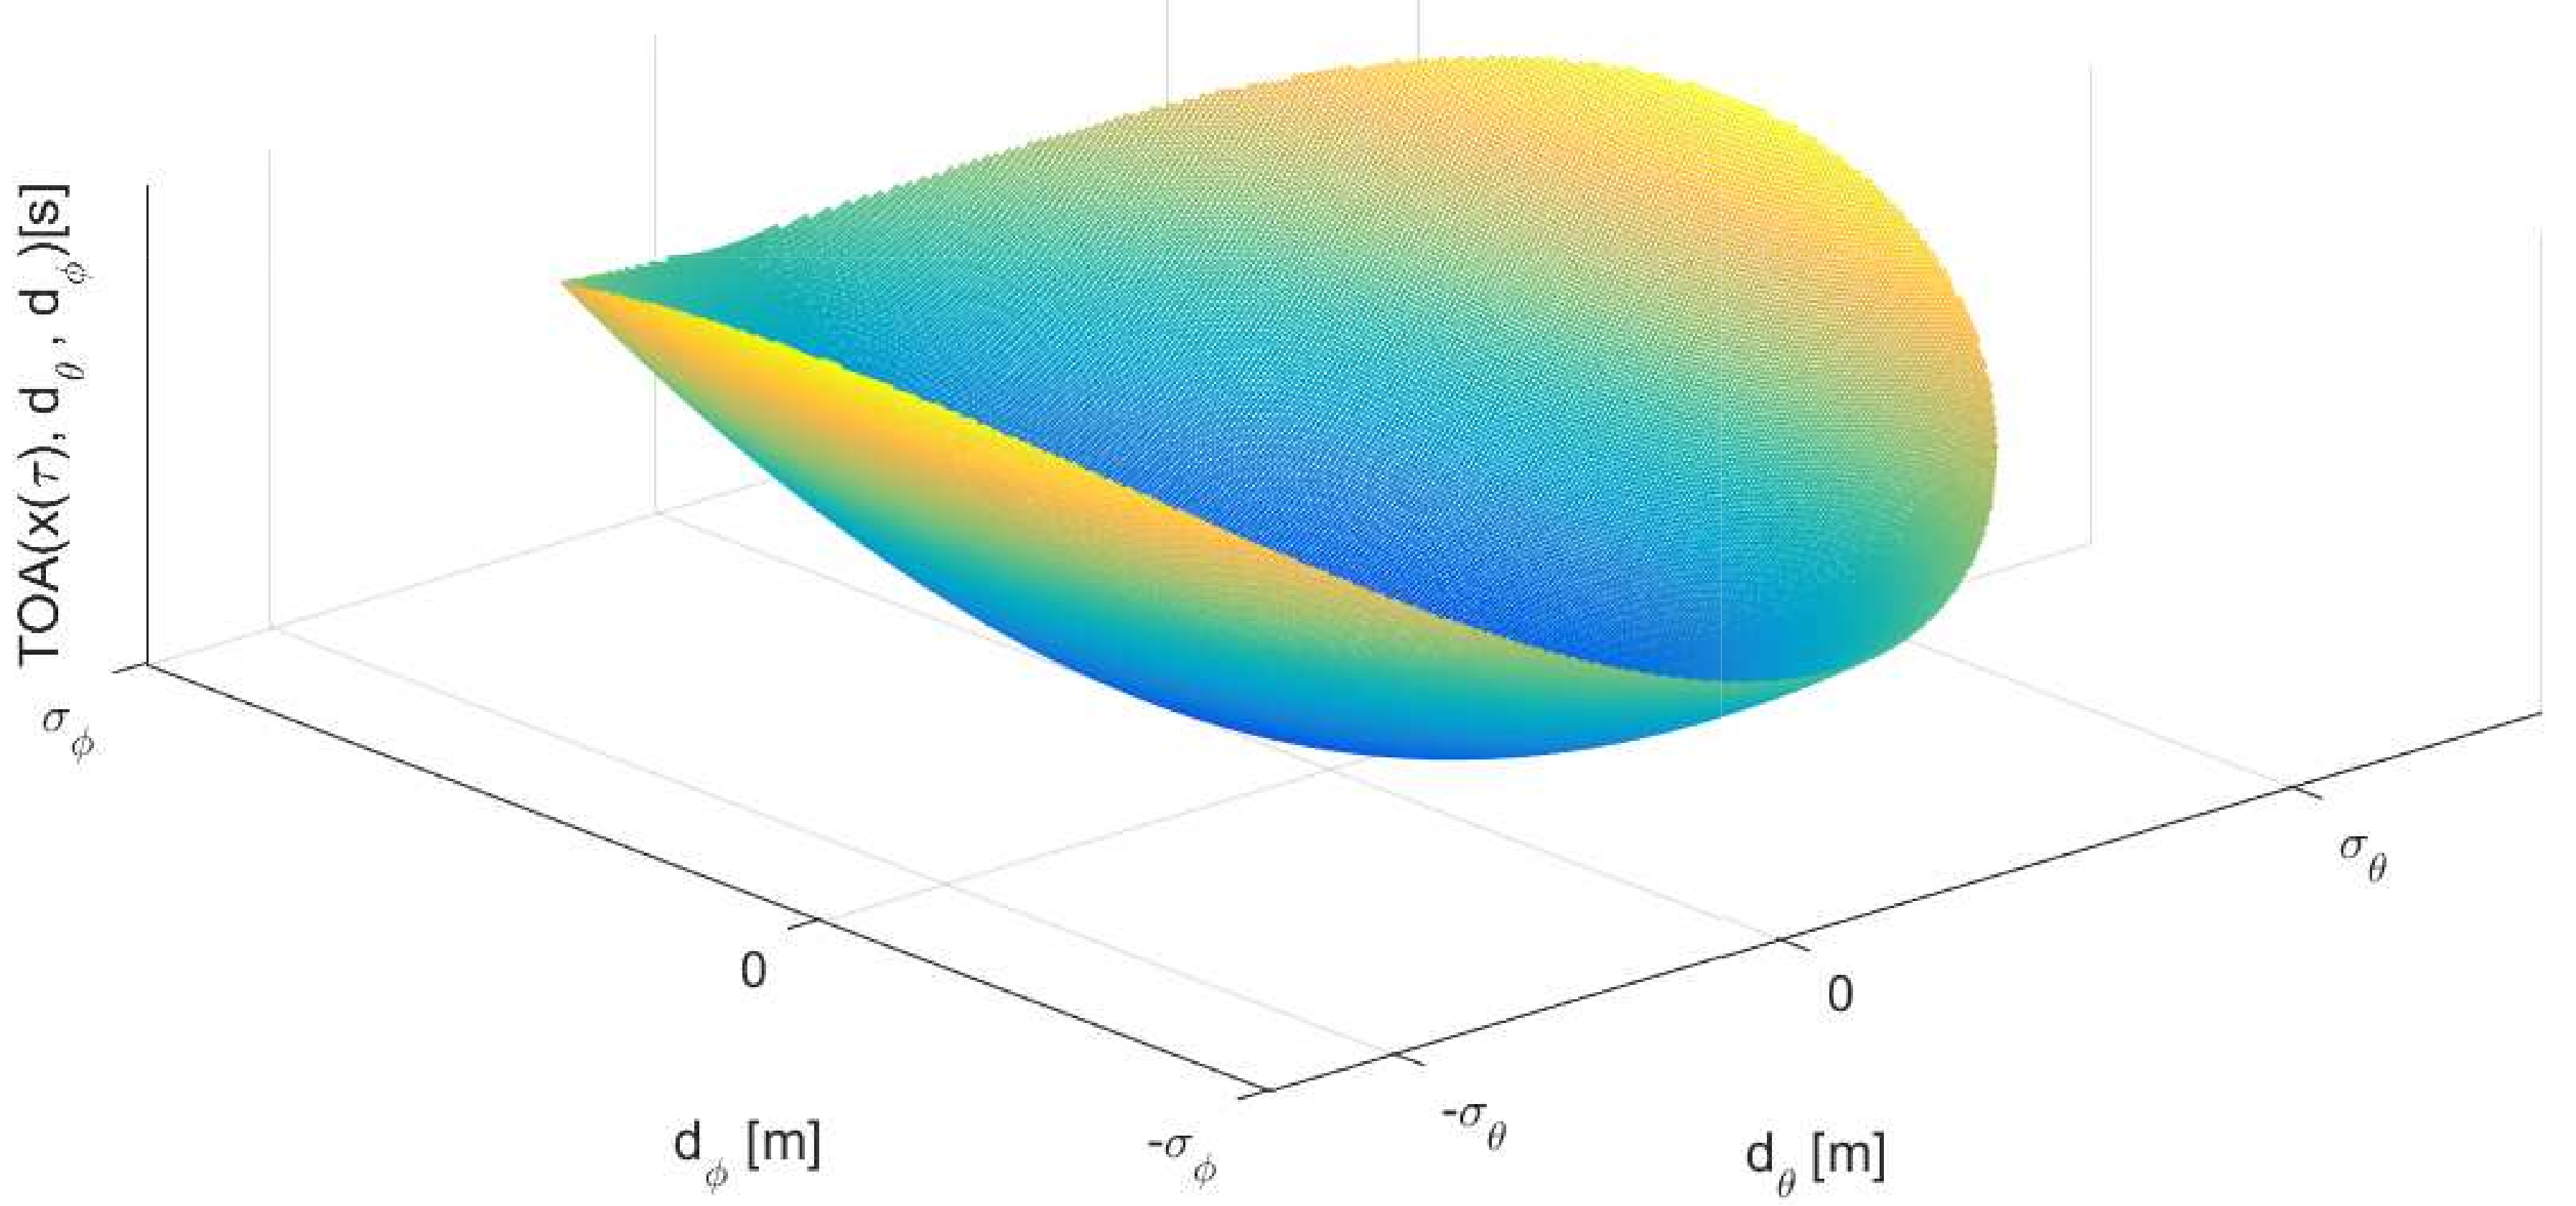
\includegraphics[width=0.7\textwidth]{\FIGDIR/P23EllipsoidCutTimeOfArrival}
    \caption{Time Of Arrival (TOA) for one ellipsoid $E_D(\vec{x}(\tau),\vec{v})$}
    \label{fig:P23EllipsoidCutTimeOfArrival}
\end{figure}
\noindent The intersection probability $P_D(\vec{x}(\tau),c_{i,j,k},\theta,\varphi)$ for one time sample $\tau$ is given by eq. \ref{eq:spreadIntersectionProbFixedtauDiscrete}, which has similar notation to eq. \ref{eq:spreadIntersectionProbFixedtau}, sums are used instead of integrals and discrete probability density function $P_D(\vec{x}(\tau),d_\theta,d_\varphi,\vec{p})$ for points form elipse and cell intersection are used as iterator base set $\vec{p}\in\left\{E_D(\vec{x}(\tau),\vec{v})\cap c_{i,j,k}\right\}$.
\begin{equation}\label{eq:spreadIntersectionProbFixedtauDiscrete}
    P_D(\vec{x}(\tau),c_{i,j,k},\theta,\varphi) =\sum_{\vec{p}\in \left\{E_D(\vec{x}(\tau),\vec{v})\cap c_{i,j,k}\right\}} P_D(\vec{x}(\tau),d_\theta,d_\varphi,\vec{p})
\end{equation}
\noindent The \emph{base intersection probability} $P_{TD}(i_k(\vec{x}_s,\vec{v},\theta,\varphi),c_{i,j,k})$ \ref{eq:spreadIntruderIntersectionProbDiscrete} is given as mean intersection probability of partial intersections $P_D(\vec{x}(\tau),c_{i,j,k},\theta,\varphi)$ where step set $T=\{$ $i_e(c_{i,j,k})$, $\dots$, $i_l(c_{i,j,k})\}$ contains all viable intersection times with ellipsoids $E(\vec{x}(\tau\in T),\vec{v})$. The denominator is basically count of samples in sample time set $T$. 
\begin{equation}\label{eq:spreadIntruderIntersectionProbDiscrete} 
    P_{TD}(i_k(\vec{x}_s,\vec{v},\theta,\varphi),c_{i,j,k})=\frac{\sum_{\tau=i_e(c_{i,j,k})}^{i_l(c_{i,j,k})} \sum_{\vec{p}\in E_D(\vec{x}(\tau),\vec{v})}P_D(\vec{x}(\tau),c_{i,j,k},\theta,\varphi,\vec{p})}{\sum_{\tau i_l(c_{i,j,k})}^{i_e(c_{i,j,k})} 1}
\end{equation}
\noindent \emph{Intersection of intruder cone and cell $c_{i,j,k}$} cell is defined by eq. \ref{eq:conicIntersectionCellIntruderDiscrete}. its a set of point $\vec{p}\in\mathscr{R}^3$ where condition of intersection between ellipsoids $E_D(\vec{x}(\tau),\vec{v})$ for times $\tau\in\mathscr{R}^+$ and cell space $c_{i,j,k}$ is met.
\begin{equation}\label{eq:conicIntersectionCellIntruderDiscrete}
    \mathscr{P}(i_k(\vec{x}_s,\vec{v},\theta,\varphi),c_{i,j,k})= \bigcup_{\forall \tau\in\mathscr{R}^+} \left\{\vec{p}\in\mathscr{R}^3:\vec{p}\in c_{i,j,k}\cap E_D(\vec{x}(\tau),\vec{v})\right\}
\end{equation}
\noindent\emph{Intruder time of entry} $i_e(i_k,c_{i,j,k})$ (\ref{eq:conicTimeOfEntryDiscrete}), for intruder $i,k$ and cell $c_{i,j,k}$ is approximated for discrete point set  $\mathscr{P}(i_k(\vec{x}_s,\vec{v},\theta,\varphi),c_{i,j,k})$ (\ref{eq:conicIntersectionCellIntruderDiscrete}) as minimal time of arrival $t_{TOA}(\vec{p})$ of member points $\vec{p}$.
\begin{equation}\label{eq:conicTimeOfEntryDiscrete}
    i_e(i_k,c_{i,j,k})\approx \min \left\{t_{TOA}(\vec{p}):\vec{p}\in\mathscr{P}(i_k(\vec{x}_s,\vec{v},\theta,\varphi),c_{i,j,k})\right\}
\end{equation}

\noindent\emph{Intruder time of leave} $i_l(i_k,c_{i,j,k})$ (\ref{eq:conicTimeOfLeaveDiscrete}), for intruder $i,k$ and cell $c_{i,j,k}$ is approximated for discrete point set  $\mathscr{P}(i_k(\vec{x}_s,\vec{v},\theta,\varphi),c_{i,j,k})$ (\ref{eq:conicIntersectionCellIntruderDiscrete}) as maximal time of arrival $t_{TOA}(\vec{p})$ of member points $\vec{p}$.
\begin{equation}\label{eq:conicTimeOfLeaveDiscrete}
    i_l(i_k,c_{i,j,k})\approx \max \left\{t_{TOA}(\vec{p}):\vec{p}\in\mathscr{P}(i_k(\vec{x}_s,\vec{v},\theta,\varphi),c_{i,j,k})\right\}
\end{equation}

\paragraph{Combined intersection model} $P_{O_I}(i_k,c_{i,j,k},l,b,s,\tau)$ is defined for intruder $i_k$ with parameters:
\begin{enumerate}
    \item\textit{Starting position} $\vec{x}_s$ - expected position of intruder $i_r$ in 3D space at time of avoidance $t_i$ in avoidance grid frame $\mathscr{A}(t_i)$.
    \item\textit{Velocity vector} $\vec{v}$ - oriented velocity of intruder $i_r$ at time of avoidance $t_i$ in avoidance grid frame $\mathscr{A}(t_i)$. 
    \item\textit{Horizontal uncertainty spread} $\theta$ - defines how much can intruder $i_r$ deviate on horizontal axis of intruder local coordinate frame (if X+ is main axis, then Y is horizontal axis in right-hand euclidean coordinate frame), due the properties of intersection definition, the horizontal uncertainty spread can have following values $\theta\in[0,\pi/2]$.
    \item\textit{Vertical uncertainty spread} $\varphi$ -defines how much can intruder $i_r$ deviate on vertical axis of intruder local coordinate frame (if X+ is main axis in local right-hand euclidean intruder coordinate frame, then Z is horizontal vertical axis), due the intersection definition, the vertical uncertainty spread can have following values $\varphi\in[0,\pi/2]$.
    \item\textit{Body volume radius} $r$ - defines the body volume of intruder in meters and it is having  $\R^+$  value.
\end{enumerate}
\noindent \emph{Flag vector} $l,b,s,\tau \in \left\{0,1\right\}$ is parametrization of probabilistic calculation: $l$ stands for \emph{lined intersection}, $b$ stands for \emph{body intersection}, $s$ stands for \emph{spread intersection}, $\tau$ stands for \emph{timed intersection}. 

\emph{Base intersection probability for line} $P_L(i_k,c_{i,j,k})$ is defined as $P_T(i_k(\vec{x},\vec{v}),c_{i,j,k})$, where $i_k$ is intruder with properties of initial position $\vec{x}$, velocity vector $\vec{v}$ and $c_{i,j,k}$ is target cell. (\ref{eq:baseIntersectionProbabilityLineIntersectionType}). \emph{Base intersection probability for body} $P_B(i_k,c_{i,j,k})$ is defined as $P_T(i_k(\vec{x},\vec{v},r),c_{i,j,k})$ (\ref{eq:baseIntersectionProbabilityBallIntersectionType}), where intruder $i_r$ has additional property of the intruder body volume $r$. \emph{Base intersection probability for spread} $P_S(i_k,c_{i,j,k})$ is defined as $P_{TD}(i_k(\vec{x}_s,\vec{v},\theta,\varphi),c_{i,j,k})$ (\ref{eq:spreadIntruderIntersectionProbDiscrete}), where intruder properties $\theta$, $\varphi$ stands for intruder horizontal and vertical uncertainty spread.

\emph{Time based intersection probability} $P_{\tau,x}(i_k,c_{i,j,k})\in[0,1]$ is defined in eq. \ref{eq:intruderIntersectionProbability}. This probability has two calculation modes, first is for 1D intersection (line), second is for volume intersection (body volume, spread elliptic cone).  Cell entry $t_e$ and leave $t_l$ time for vehicle in avoidance grid $\mathscr{A}(t_i)$ are given by eq. \ref{eq:cellEntryTime} and \ref{eq:cellLeaveTime}. Intruder leave and entry time for 1D intersections is trivial and is omitted in this section. Intruder entry $i_e$ and intruder leave $i_l$ for 3D intersection are given by eq. \ref{eq:conicTimeOfEntryDiscrete} and \ref{eq:conicTimeOfLeaveDiscrete}. All partial probabilities with respective definition references are summarized in eq. \ref{eq:partialProbabilitiesIntruderSummary}

\begin{equation}\label{eq:partialProbabilitiesIntruderSummary}
    \begin{aligned}
        P_L(i_k,c_{i,j,k}) &= P_T(i_k(\vec{x},\vec{v}),c_{i,j,k}) &(\ref{eq:baseIntersectionProbabilityLineIntersectionType})\\
        P_B(i_k,c_{i,j,k}) &= P_T(i_k(\vec{x},\vec{v},r),c_{i,j,k}) &(\ref{eq:baseIntersectionProbabilityBallIntersectionType})\\
        P_S(i_k,c_{i,j,k}) &= P_{TD}(i_k(\vec{x}_s,\vec{v},\theta,\varphi),c_{i,j,k}) &(\ref{eq:spreadIntruderIntersectionProbDiscrete})\\
        P_{\tau,x}(i_k,c_{i,j,k})&=\frac{\norm{[i_e(c_{i,j,k}),i_l(c_{i,j,k})]\cap [t_e,t_l]}}{\norm{[t_e,t_l]}}& (\ref{eq:intruderIntersectionProbability})\\
    \end{aligned}
\end{equation}
\noindent With definition of all base and timed probabilities (\ref{eq:partialProbabilitiesIntruderSummary}) and given flag vector $l,b,s,\tau \in\left\{0,1\right\}$ one can formulate final intersection probability $P_{O_I}(i_k,c_{i,j,k},l,b,s,\tau)$ (\ref{eq:intruderInCellProbabilityOneIntruder}) for intruder $i_k$ and cell $c_{i,j,k}$. The principle is following: \emph{maximum of selected probabilities product based on flag vector is final probability of intruder $i_k$ in cell}. The time-based flag $\tau$ is adding timed probability $P_{\tau,x}(i_k,c_{i,j,k})$, where time intersection probability is defined by $x=\left\{L,B,S\right\}$ for line, body volume, spread ellipse time intersections ($P_{\tau,L}(i_k,c_{i,j,k})$ $\neq$ $P_{\tau,B}(i_k,c_{i,j,k})$ $\neq$ $P_{\tau,B}(i_k,c_{i,j,k})$ for one intruder $i_k$).

\begin{equation}\label{eq:intruderInCellProbabilityOneIntruder}
    \begin{aligned}
        P_{O_I}(i_k,c_{i,j,k},l,b,s,\tau) & = \begin{cases}\tau=0&:\max\left\{\begin{aligned}P_L(i_k,c_{i,j,k}).l\\ P_B(i_k,c_{i,j,k}).b\\P_S(i_k,c_{i,j,k}).s\end{aligned}\right\}\\\tau=1&:\max\left\{\begin{aligned}P_{\tau,L}(i_k,c_{i,j,k}).P_L(i_k,c_{i,j,k}).l\\ P_{\tau,B}(i_k,c_{i,j,k}).P_B(i_k,c_{i,j,k}).b\\P_{\tau,S}(i_k,c_{i,j,k}).P_S(i_k,c_{i,j,k}).s\end{aligned}\right\}\end{cases} &\\
    \end{aligned}
\end{equation}

\paragraph{Intruder obstacle probability} $P_{O_I}(c_{i,j,k})$ is defined for set of intruders $\mathscr{I}(\mathscr{A}(t_i))$ containing all detected intruders $i_r\in\mathscr{I}$ in avoidance grid $\mathscr{A}(t_i)$ for time of avoidance $t_i$. The equation \ref{eq:intruderInCellProbability} is simple inverted cumulative product of partial intruder in cell probabilities $P_{O_I}(i_k,c_{i,j,k},l,b,s,\tau)$ (\ref{eq:intruderInCellProbabilityOneIntruder}). The principle is simple, if there is one intruder in cell, cumulative probability remains the same $1-(1-P_{O_I}(i_k,c_{i,j,k},l,b,s,\tau))$ = $P_{O_I}(i_k,c_{i,j,k},l,b,s,\tau)$. If there is multiple intruders $i_1,i_2,\dots,i_k,k\in\N^+$, the probability of collision is geometrically increasing, even with small probability for some intruders $i_k$.

\begin{equation}\label{eq:intruderInCellProbability}
    P_{O_I}(c_{i,j,k}) = 1-\left(\prod_{i_k\in\mathscr{I}(\mathscr{A}(t_i))}1-P_{O_I}(i_k,c_{i,j,k},l,b,s,\tau)\right)
\end{equation}

\section{Detected obstacle probability}\label{sec:detectedObstacleProbability}
\noindent Probability of detected obstacle $P_{O_D}$ describes how probable is to encounter detected obstacle in cell $c_{i,j,k}$. Probability of detected obstacle is merged information. Let say that obstacle can be detected by various sensors $s_1,\dots,s_i,i\in\N^+$, with partial obstacle certainty $P_{O_D}(s_k,c_{i,j,k})$, then cumulative probability of obstacle is given by:
\begin{equation}\label{eq:detectedObstacleProbability}
    P_{O_D}(c_{i,j,k})= 1- \left\{\prod_{s_k\in s_1,\dots,s_i}^{i\in\N^+}\left(1-P_{O_D}(s_k,c_{i,j,k})\right)\right\}
\end{equation}
\noindent Final detected obstacle probability $P_{O_D}(c_{i,j,k})$ is given as inverted cumulative probability $P_{O_D}(s_k,c_{i,j,k})$ of partial probabilities for sensor array $s_k\in s_1,\dots,s_i,i\in\N^+$.

\paragraph{Probability of obstacle occurrence in case of LiDAR sensor}, for this case $s_k$ is fixed and its set as homogeneous two axis rotary LiDAR. For one cell $c_{i,j,k}$ there exists set of passing LiDAR beams:
\begin{equation}
    \mathscr{L}(c_{i,j,k})=\left\{[\theta\in\Theta,\varphi\in\Phi]\in\R^2:\begin{aligned} &c_{i,j,k}.\theta_s\le\theta\le c_{i,j,k}.\theta_e\\&c_{i,j,k}.\varphi_s\le\varphi\le c_{i,j,k}.\varphi_e \end{aligned}\right\}
\end{equation}
\noindent The pair $[\theta,\varphi]$ is in homogeneous offset system given by product of discrete set of horizontal angles offsets $\Theta$ and discrete set of vertical angles offsets $\Phi$. The set $\mathscr{L}(c_{i,j,k})$ is finite countable and nonempty for any $c_{i,j,k}$, otherwise definition of avoidance grid $\mathscr{A}(t_i)$ needs to be changed.

The hit function $h:\mathscr{L}(c_{i,j,k})\times\R^n\to[0,\infty]$ returns a distance of single beam return for beam passing trough $[\theta,\varphi]\in\mathscr{L}(c_{i,j,k})$ angle offsets with vehicle state space $\vec{x}\in\R^n$. Then set of LiDAR hits $\mathscr{H}$ in cell $c_{i,j,k}$ at system state $\vec{x}$ is given as follow:
\begin{equation}
    \mathscr{H}(\vec{x},c_{i,j,k})=\left\{[d,\theta,\varphi]\in\R^3: \begin{aligned}&c_{i,j,k}.d_s\le d \le c_{i,j,k}.d_e\\ &\forall [\theta,\varphi]\in\mathscr{L}(c_{i,j,k})\\&d=h(\mathscr{L}(c_{i,j,k}),[\theta\varphi])\\\end{aligned}\right\}
\end{equation}

\noindent Probability of obstacle in case of LiDAR detection $P_{O_L}$ is given as ratio between landed hits and possible hits:
\begin{equation}
    P_{O_L}(\vec{x},c_{i,j,k})=\frac{|\mathscr{H}(\vec{x},c_{i,j,k})|}{|\mathscr{L}(c_{i,j,k})|}
\end{equation}


\noindent Probability of vision hindrance $P_{V_H}$ is given as supplement to probability of obstacle:
\begin{equation}\label{eq:probabilityOfVisibilityHindrance}
    P_{V_H}(\vec{x},c_{i,j,k})=1-\frac{|\mathscr{H}(\vec{x},c_{i,j,k})|}{|\mathscr{L}(c_{i,j,k})|}
\end{equation}

\paragraph{Cell density function.}
\noindent Let`s start with differential form of cell surface calculation eq. \ref{eq:finalCellSquare}. The target object have several hits in given cell Avoidance grid $\mathscr{A}$ cell $c_{i,j,k}$. Cell $c_i,j,k$ have following properties which are used in surface calculation:
\begin{enumerate}
    \item \textit{Horizontal span} ($\theta_s$, $\theta_e$) - defines range of horizontal scanner partition.
    \item \textit{Vertical span} ($\varphi_s$, $\varphi_e$) - defines range of vertical scanner partition.
\end{enumerate}

\noindent By rewriting eq. \ref{eq:finalCellSquare}. and using $\theta$ as horizontal range parameter and $\varphi$ as inverted vertical range parameter following surface integral is proposed:
\begin{equation}
    \int_{\theta_s}^{\theta_e}\int_{\varphi_s}^{\varphi_e} \text{d}A \quad \text{d}\varphi\text{d}\theta = \int_{\theta_s}^{\theta_e}\int_{\varphi_e}^{\varphi_s} r^2 \cos(\varphi) \quad \text{d}\varphi\text{d}\theta
\end{equation}

\noindent Numerical stable integration exist for boundaries $\theta \ in [-\pi,\pi]$ $\varphi \in [0,\frac{pi}{2}]$ and is given by following equation:

\begin{equation}\label{eq:intersectionSurfaceForCell}
    A(r,\theta_s,\theta_e,\varphi_s,\varphi_e) = \left\{
    \begin{aligned}
        \varphi_s<0, \varphi_e\le0 :& r^2(\sin |\varphi_s| - \sin|\varphi_e|)(\theta_e-\theta_s)\\
        \varphi_s<0, \varphi_e>0   :& r^2(\sin |\varphi_s| + \sin|\varphi_e|)(\theta_e-\theta_s)\\
        \varphi_s\ge 0 \varphi_e<0 :& r^2(\sin \varphi_e - \sin\varphi_s)(\theta_e-\theta_s)
    \end{aligned}
    \right.
\end{equation}

\noindent Intersection surface for cell $A_C$ is then given by eq. \ref{eq:intersectionSurfaceForCell}. Most of the LiDAR scanners have \textit{Points per rotation parameter [ppr]}. $P_S[p/2\pi]$Let`s  assume that scanning density is homogeneous. The covered area at distance $r$ for one LiDAR swipe $A_S$ is given by eq. \ref{eq:intersectionSurfaceForCell}. where $\theta_s=\pi$, $\theta_e=\pi$, for full swipe and $\varphi_s$, $\varphi_e$ set to maximal horizontal range. Then for object with frontal area surface $A_O$, the minimal hit count $P_O$ is given as:
\begin{equation}\label{eq:lidarHitFormula}
    P_{O_D} = \textit{min} \left\{P_S\frac{A_O}{A_S},P_S\frac{A_C}{A_S}\right\}
\end{equation}

\noindent \textit{LiDAR hit formula} (\ref{eq:lidarHitFormula}) covers hit count for cell $c_{i,j,k}$ and object $O$ of any size $A$ and any detection distance $r$.

\section{Visibility probability}\label{sec:visibilityProbability}
\noindent For each cell $c_{i,j,k}$ and each sensor $s_k$ there exist hindrance of vision probability $P_{V_H}$, which defines how much vision is clouded in single cell. Example of hindrance calculation for LiDAR has been given by eq. \ref{eq:probabilityOfVisibilityHindrance}. Let us consider cell row $\mathscr{C}(j_{fix},k_{fix})$ with fixed horizontal index $j_fix$ and vertical index $k_{fix}$ is given as series of:
\begin{equation}\label{eq:cellrowDefinition}
    \mathscr{C}(j_{fix},k_{fix})= \left\{c_{i,j,k}\in\mathscr{A}(t_i):i\in\{1,..,a\},j=j_{fix},k=k_{fix}\right\}
\end{equation}
For each cell $c_{i,j,k}$ there exists a function which calculates final visibility hindrance probability $P_{V_F}(c_{i,j,k},\mathscr{S})$, where $\mathscr{S}$ is set of sensors providing hindrance rate. Then for ordered cell row $\mathscr{C}(j_{fix},k_{fix})=\left\{c_{1,j_{fix},k_{fix}}, c_{2,j_{fix},k_{fix}}, \dots,c_{a,j_{fix},k_{fix}}\right\}, a\in\N^+$ and for one selected cell $c_{i,j,k}$ the probability of visibility is given as supplement to hindrance from previous cells. The equation for this statement holds as follows:
\begin{equation}\label{eq:FinalVisibilityProbability}
    P_{V}(c_{i_c,j_c,k_c},\mathscr{S})= 1 - \sum_{a\in\N^+}^{a<i_c} P_{V_F}(c_{a,j_c,k_c},\mathscr{S}),\quad c_{a,j_c,k_c}\in\mathscr{C}(j_{c},k_{c})
\end{equation}

\noindent For example cell $c_{4,j_{fix},k_{fix}}$ is selected for visibility calculation $P_{V}(c_{4,j_{fix},k_{fix}})$, then cells $c_{1,j_{fix},k_{fix}}$, $c_{2,j_{fix},k_{fix}}$, and $c_{3,j_{fix},k_{fix}}$, are used as a base of calculation for visibility hindrance probability $P_{V_F}$.

\noindent \emph{The maximum hindrance} for any cell row $|{C}(j_{fix},k_{fix})|=k\in \N^+$ with  boundary:
\begin{equation}
    0 \le \sum_{c\in{C}(j_{fix},k_{fix})} P_{V_F}(c) \le 1
\end{equation}

\noindent For one cell row $\mathscr{C}(j_{fix},k_{fix})$, where count of layers is equal to 10, and layers have equal spacing. There is defined sensor field $\mathscr{S}=\left\{s_1\right\}$, where $s_1$ is LiDAR sensor. 

During consequent LiDAR scans $s(t_0)$, $s(t_1)$, $s(t_2)$, and $s(t_3)$ the obstacle sets $\mathscr{O}_1(t_1)=\{o_1\}$, $\mathscr{O}_2(t_2)=\{o_1,o_2\}$, and $\mathscr{O}_3(t_3)=\{o_1,o_2,o_3\}$ are discovered. Assigned hindrance probabilities are like follow:
\begin{itemize}
    \item\emph{Time $t_0$} (fig. \ref{fig:P24VisibilityFreeSpace}) - there is no obstacle nor hindrance, all cells are free
    \item\emph{Time $t_1$} (fig. \ref{fig:P25VisibilityFirstObstacle}) - $\mathscr{O}_1(t_1)=\{o_1\}$ was detected, the hindrance probability $P_{V_F}$ $(c_{3,j_{fix},k_{fix}})$ is equal to $0.25$. The visibility in cells $c_{4-10,j_{fix},k_{fix}}$ is 75 percent now. 
    \item\emph{Time $t_2$} (fig. \ref{fig:P26VisibilitySecondObstacle}) - $\mathscr{O}_2(t_2)=\{o_1,o_2\}$ was detected, the additional hindrance probability  $P_{V_F}(c_{5,j_{fix},k_{fix}})$ is $0.15$. The visibility in cells $c_{6-10,j_{fix},k_{fix}}$ is lowered by additional 15 percent and its set to 60 percent now.
    \item\emph{Time $t_3$} (fig. \ref{fig:P27VisibilityThirdObstacle}) - $\mathscr{O}_3(t_3)=\{o_1,o_2,o_3\}$  was detected the additional hindrance probability  $P_{V_F}(c_{7,j_{fix},k_{fix}})$ is $0.20$. The visibility in cells $c_{8-10,j_{fix},k_{fix}}$ is lowered by additional 20 percent and its set to 40 percent now.
\end{itemize}

\noindent The vehicle is detecting in avoidance grid $\mathscr{A}(t_0)$ and do not detected any obstacles (fig. \ref{fig:P24VisibilityFreeSpace}). The cell row $\mathscr{C}(j_{fix},k_{fix})$ is completely visible.
\begin{figure}[H]
    \centering
    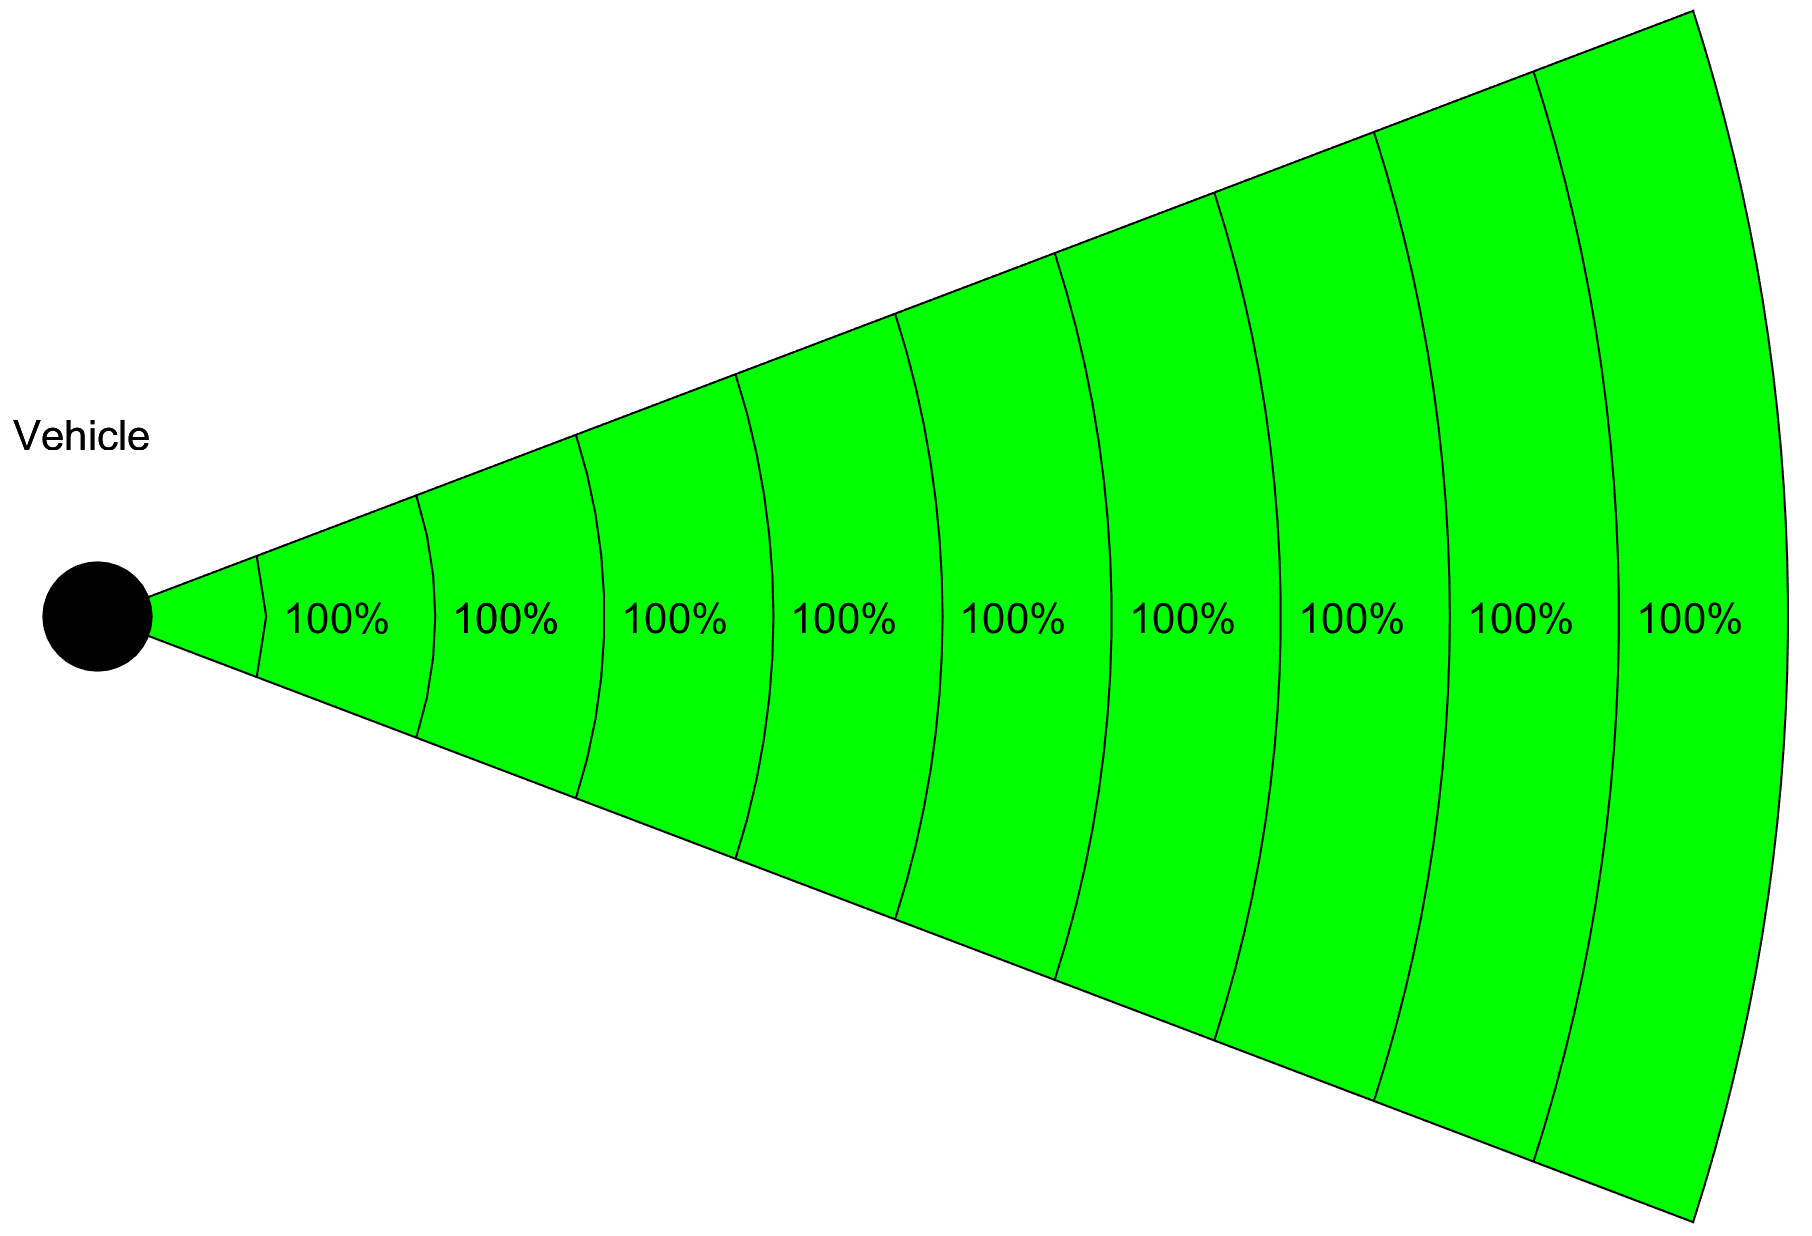
\includegraphics[width=0.7\textwidth]{\FIGDIR/P24VisibilityFreeSpace}
    \caption{Visibility probability for cell row - free space}
    \label{fig:P24VisibilityFreeSpace}
\end{figure}

\noindent The vehicle is detecting in avoidance grid $\mathscr{A}(t_1)$ and detects one obstacle $O_1$ (fig. \ref{fig:P25VisibilityFirstObstacle}). The obstacle is placed in third cell from vehicle. Note that visibility of third cell is 100 percent, because no prior hindrance in line of sight exist. 
\begin{figure}[H]
    \centering
    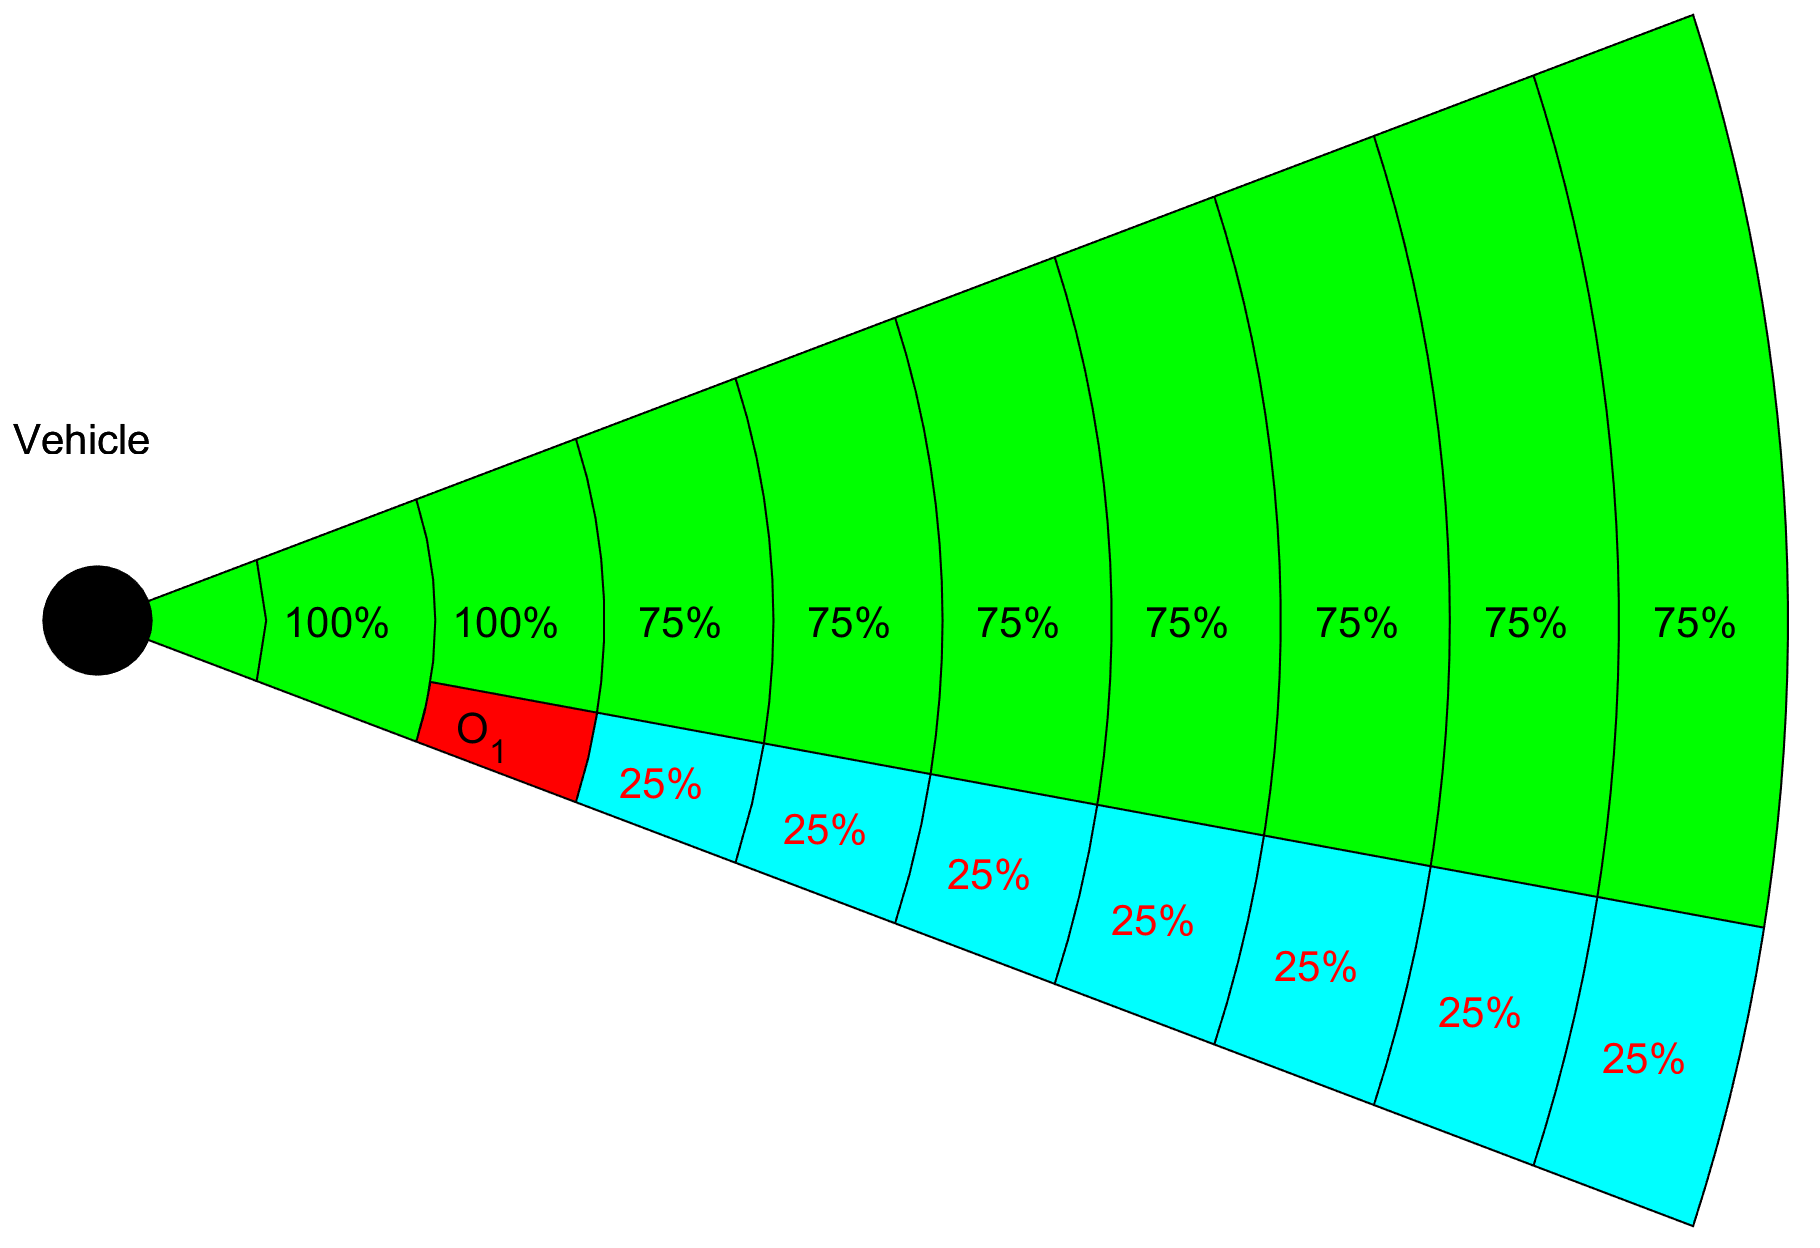
\includegraphics[width=0.7\textwidth]{\FIGDIR/P25VisibilityFirstObstacle}
    \caption{Visibility probability for cell row - first obstacle}
    \label{fig:P25VisibilityFirstObstacle}
\end{figure}

\noindent The vehicle is detecting in avoidance grid $\mathscr{A}(t_2)$ detects obstacles $O_1$, $O_2$ (fig. \ref{fig:P26VisibilitySecondObstacle}). The cell row $\mathscr{C}(j_{fix},k_{fix})$ is now  hindered with obstacles $O_1$ with hindrance $0.25$ and obstacle $O_2$ with hindrance $0.15$.
\begin{figure}[H]
    \centering
    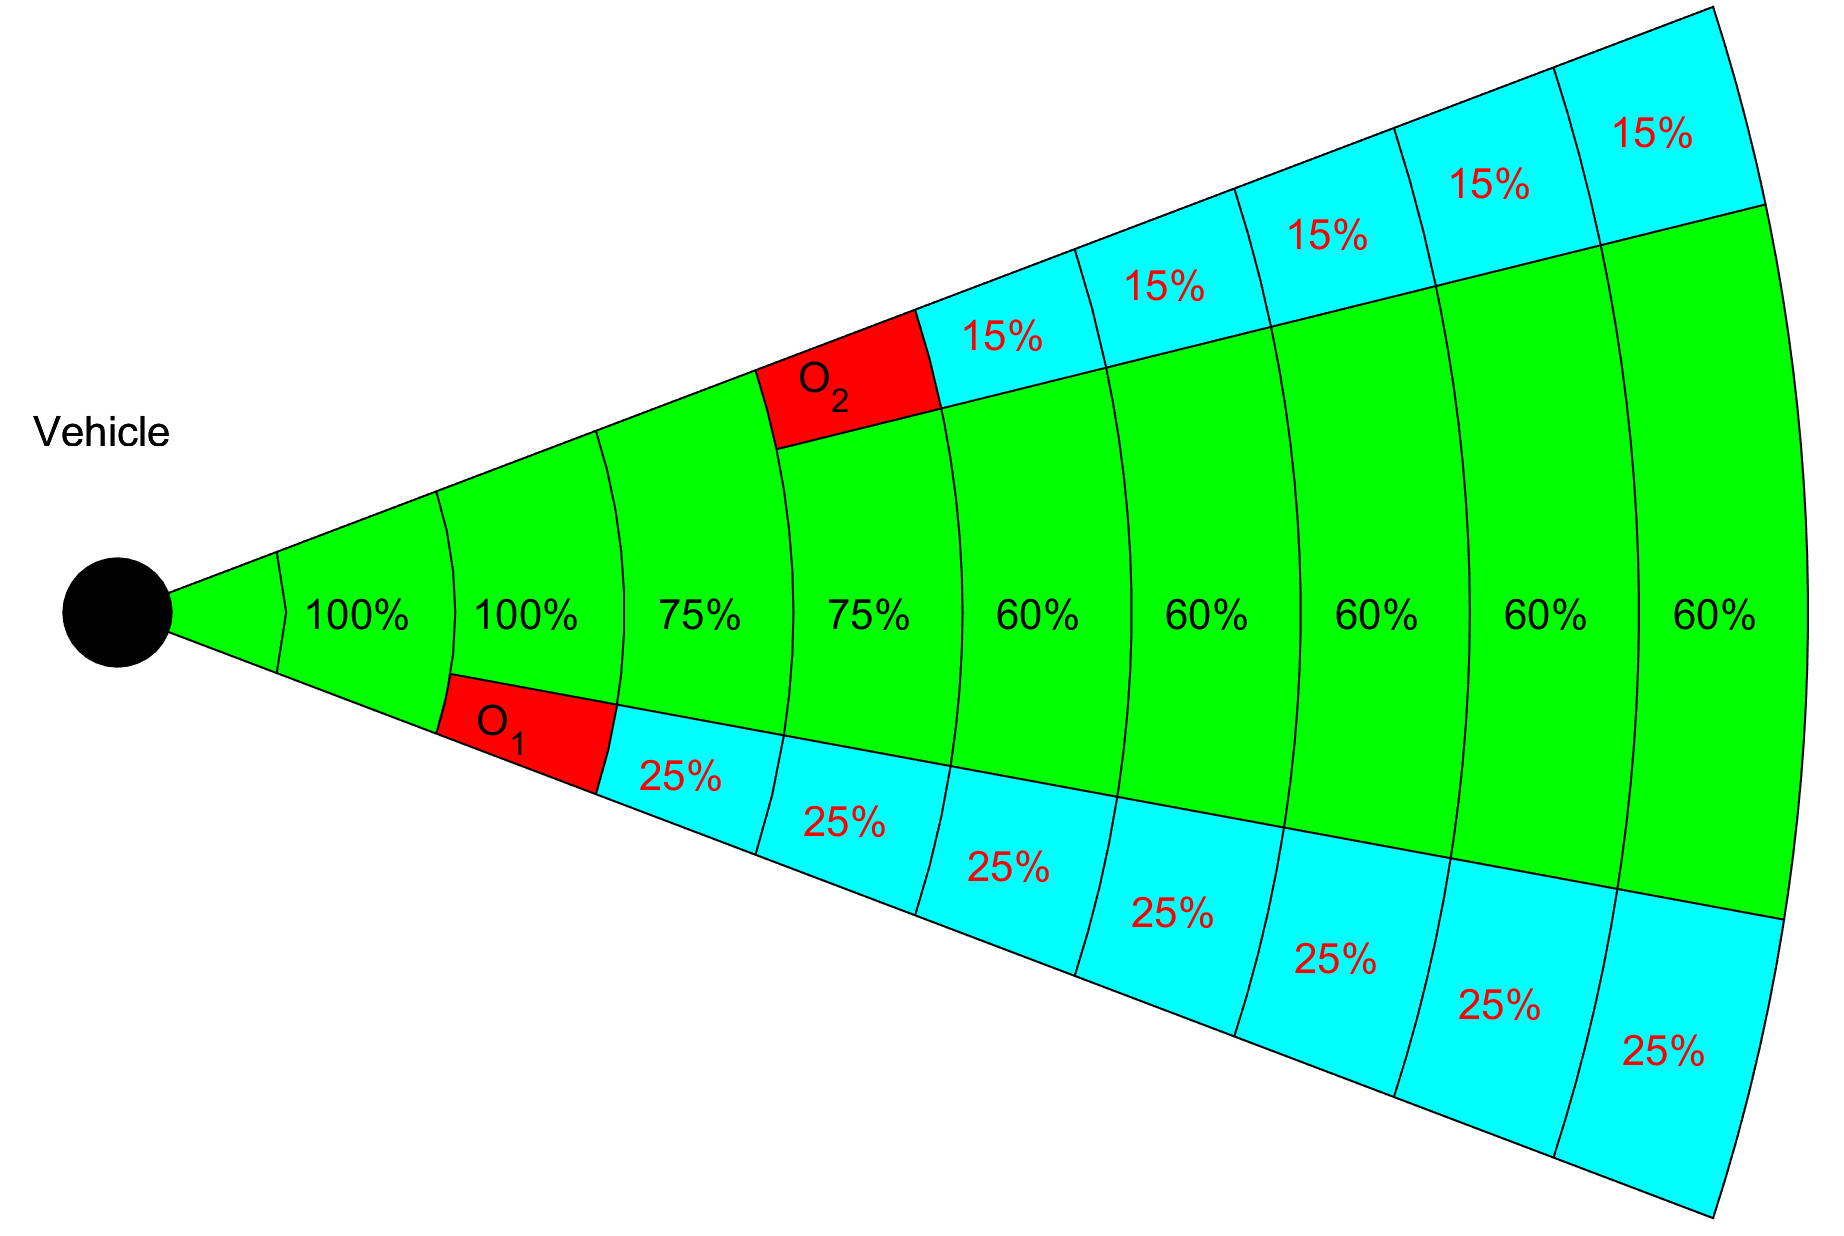
\includegraphics[width=0.7\textwidth]{\FIGDIR/P26VisibilitySecondObstacle}
    \caption{Visibility probability for cell row - second obstacle}
    \label{fig:P26VisibilitySecondObstacle}
\end{figure}

\noindent The vehicle is detecting in avoidance grid $\mathscr{A}(t_3)$ detects obstacles $O_1$, $O_2$, $O_3$ (fig. \ref{fig:P27VisibilityThirdObstacle}). The cell row $\mathscr{C}(j_{fix},k_{fix})$ is now  hindered with obstacles $O_1$ with hindrance $0.25$, obstacle $O_2$ with hindrance $0.15$, and obstacle $O_3$ with hindrance $0.20$.
\begin{figure}[H]
    \centering
    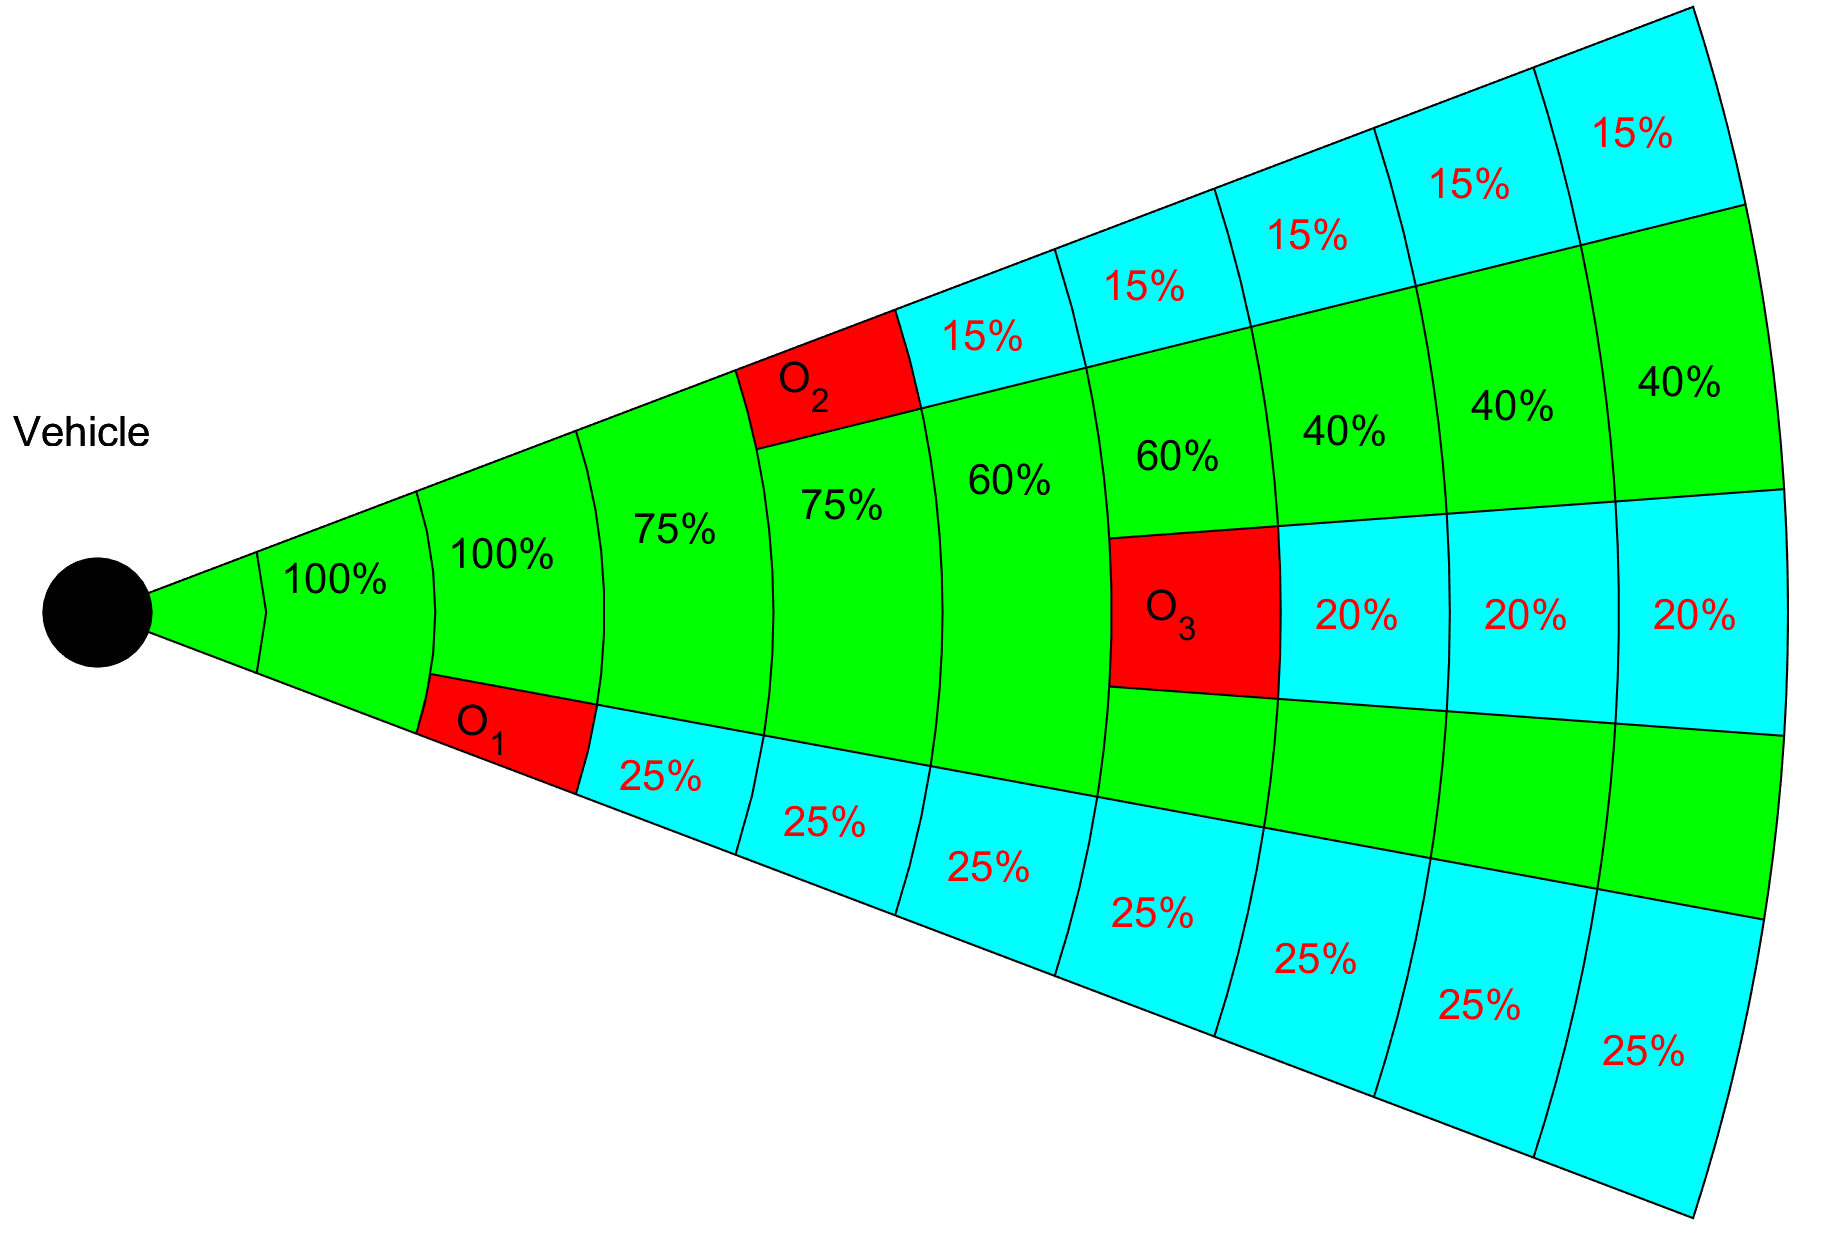
\includegraphics[width=0.7\textwidth]{\FIGDIR/P27VisibilityThirdObstacle}
    \caption{Visibility probability for cell row - third obstacle}
    \label{fig:P27VisibilityThirdObstacle}
\end{figure}

\section{Map obstacle probability}\label{sec:mapObstacleProbability}
\noindent\emph{Probability of Map Obstacle} $P_{O_M}$ occurrence follows very simple logic. There are three possible cases:

\noindent\emph{Map obstacle $O_M$} is charted on map (fig. \ref{fig:P28MapObstacleUndetected}), but is undetected by any sensor in sensor set $\mathscr{S}$. Therefore the probability of map obstacle occurrence is equal to $0$.
\begin{figure}[H]
    \centering
    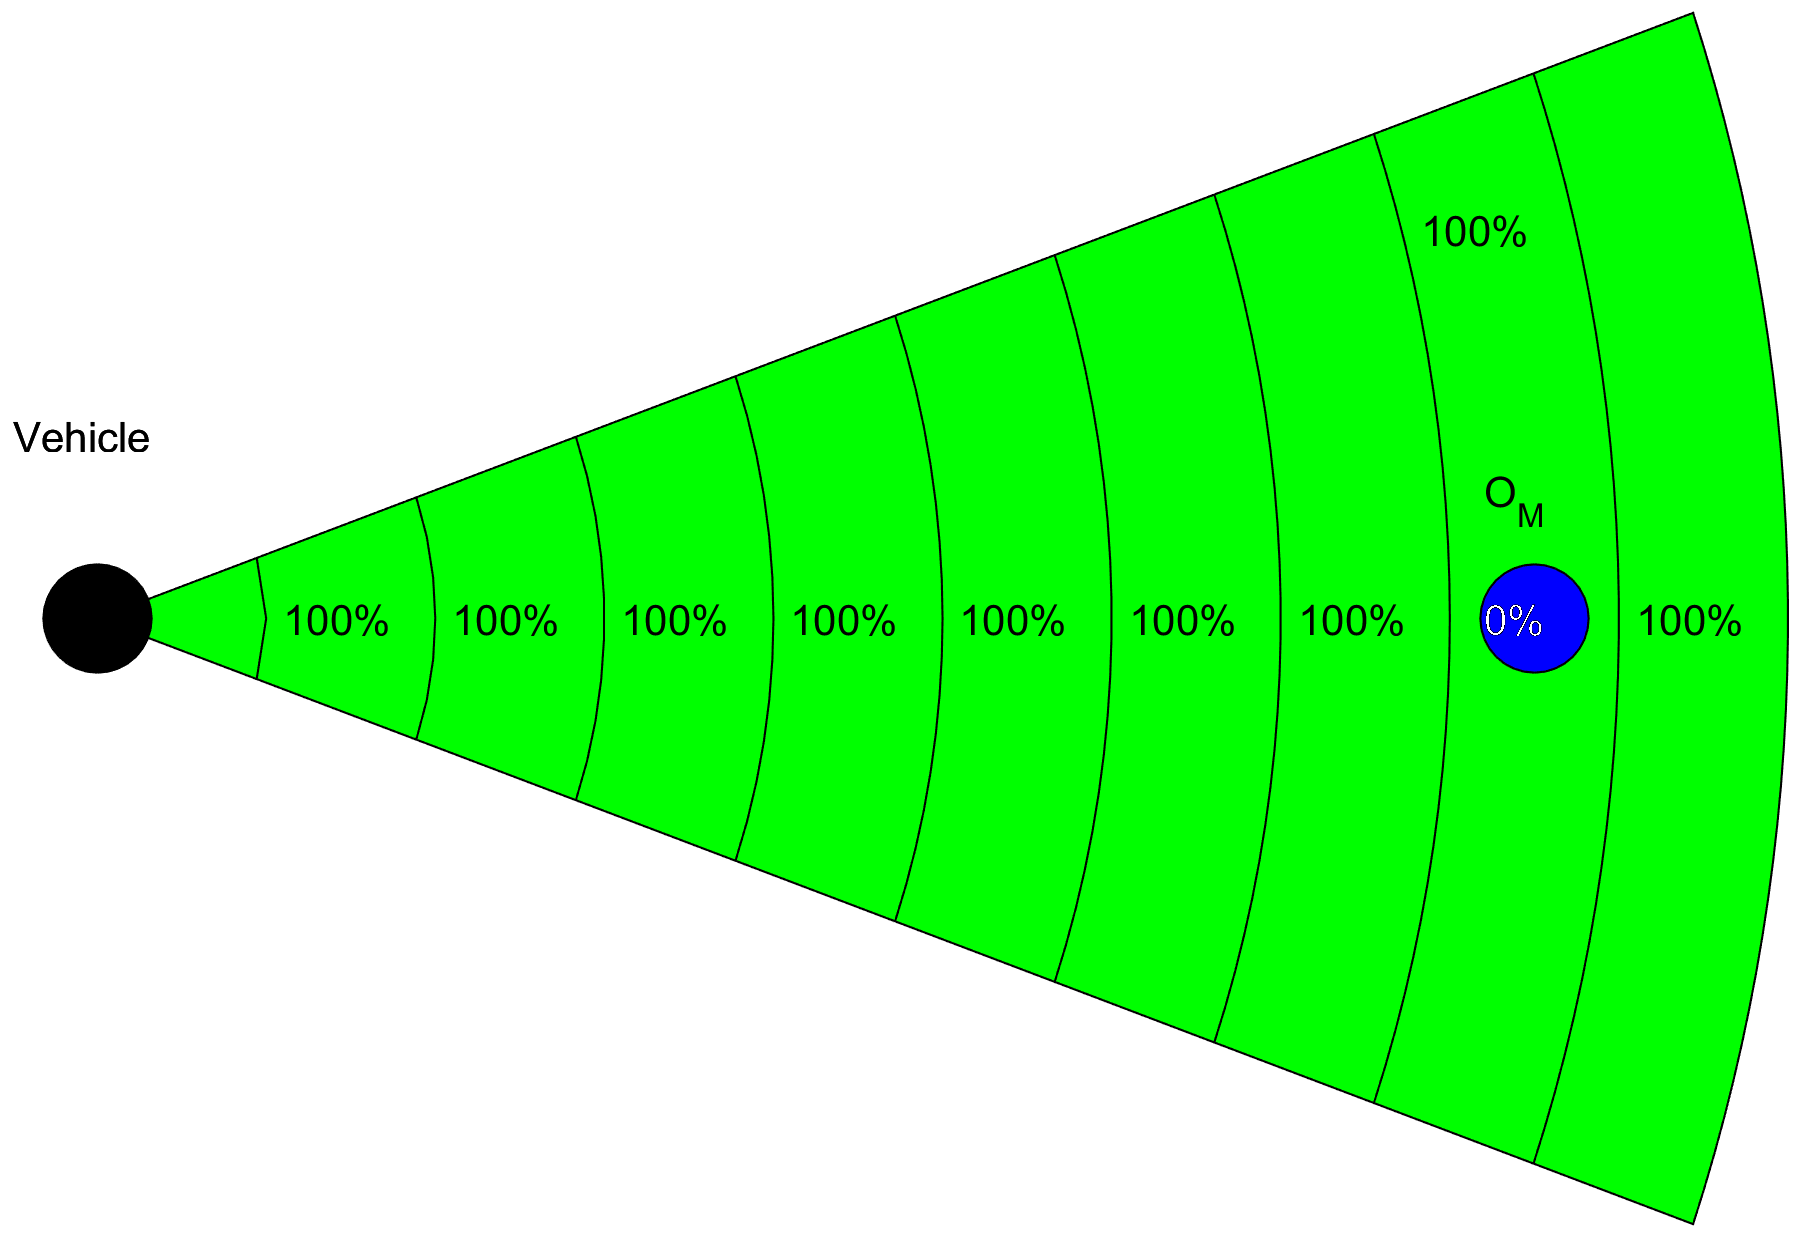
\includegraphics[width=0.7\textwidth]{\FIGDIR/P28MapObstacleUndetected}
    \caption{Map obstacle - undetected by sensory system}
    \label{fig:P28MapObstacleUndetected}
\end{figure}

\noindent\emph{Map obstacle $O_M$} is charted on map and detected by any sensor in sensor system $\mathscr{S}$ (fig. \ref{fig:P29MapObstacleDetected}). The probability of map obstacle $P_{O_M}$ is equal to probability of detected obstacle $P_{O_D}$, therefore its equal to $1$.

\begin{figure}[H]
    \centering
    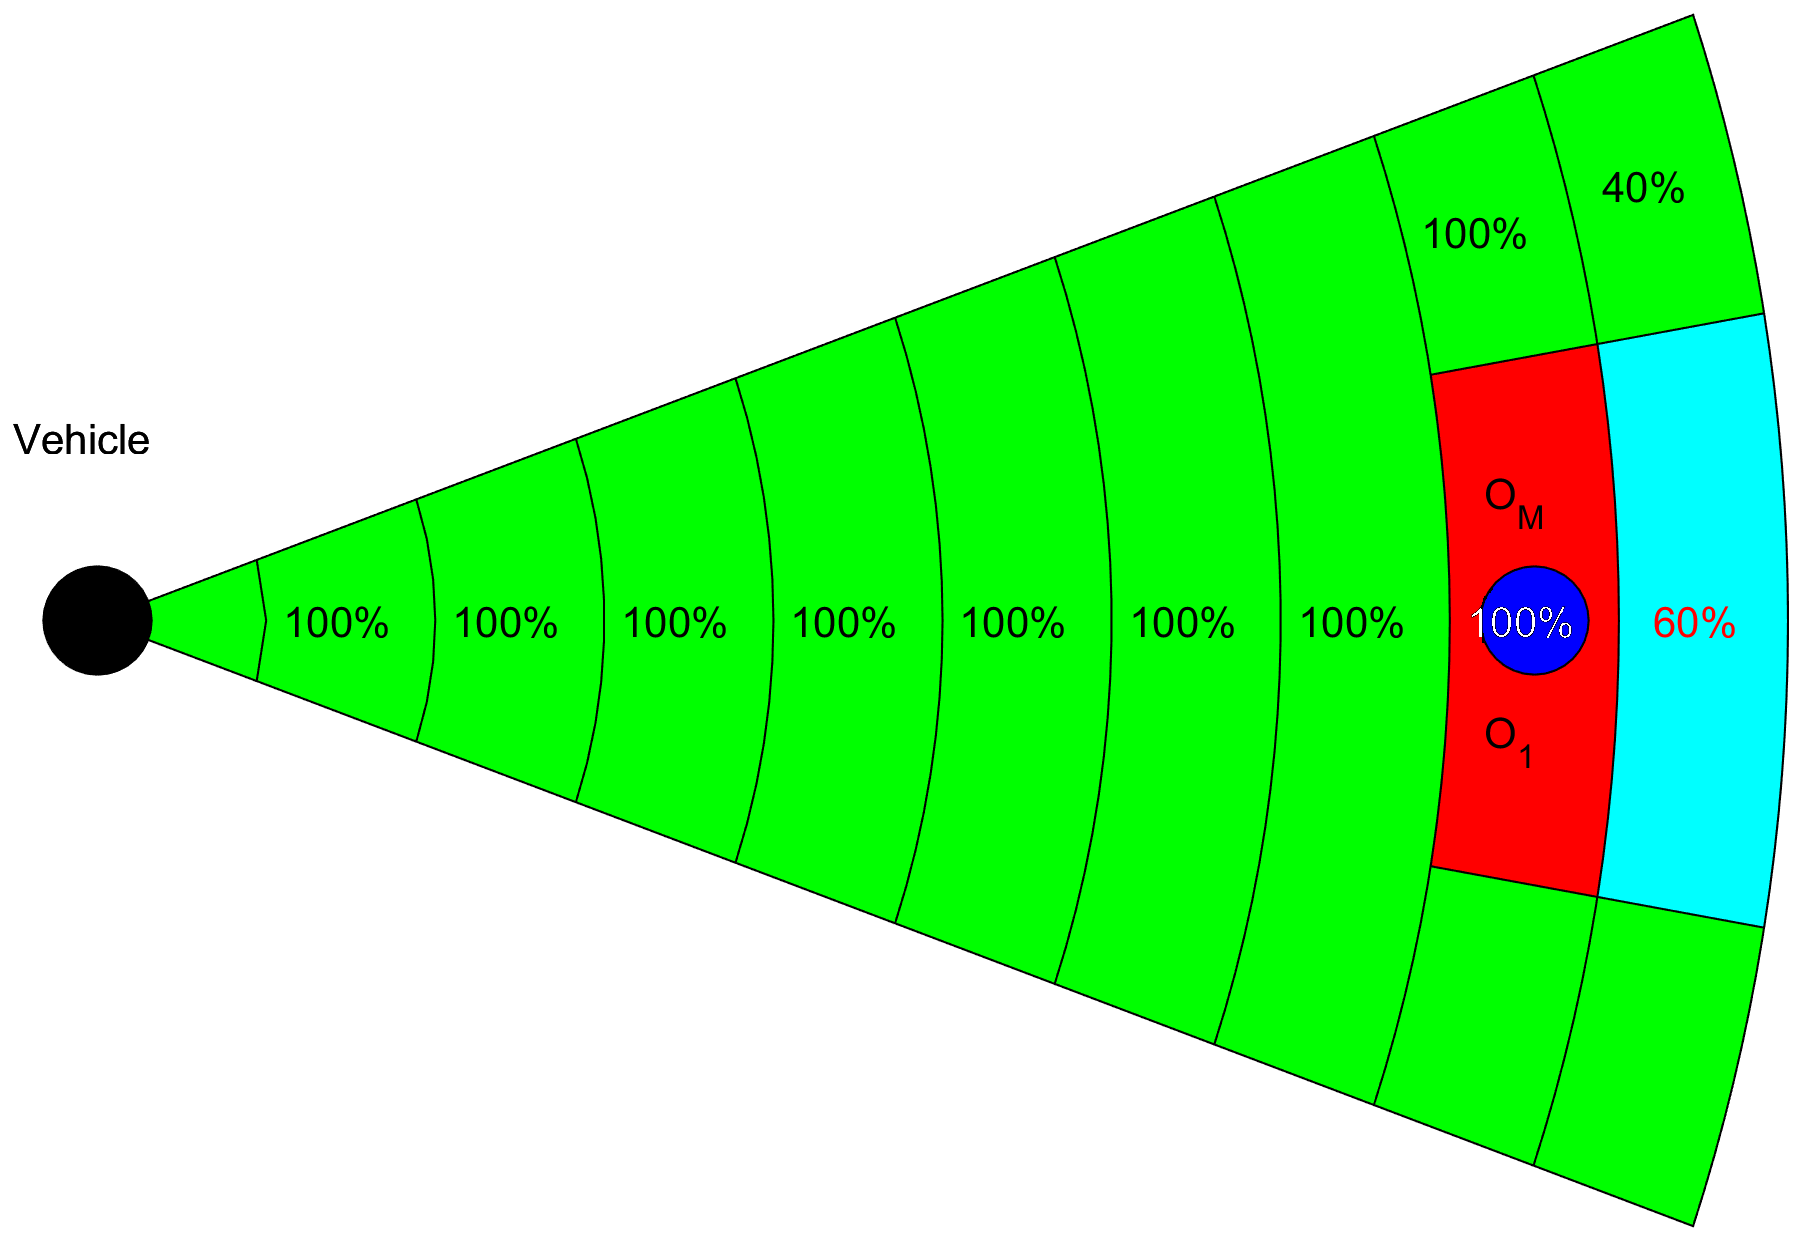
\includegraphics[width=0.7\textwidth]{\FIGDIR/P29MapObstacleDetected}
    \caption{Map obstacle - detected by sensory system}
    \label{fig:P29MapObstacleDetected}
\end{figure}

\noindent\emph{Map obstacle $O_M$} is hindered behind other detected obstacle $O_1$ (fig. \ref{fig:P30MapObstacleHiden}). The detected obstacle $O_1\in\mathscr{O}_D$ is in cell $c_{i,j,k}$ and is reducing visibility in follow up cells $c_{i_f>i,j,k}$ by $60$ percent.
\begin{figure}[H]
    \centering
    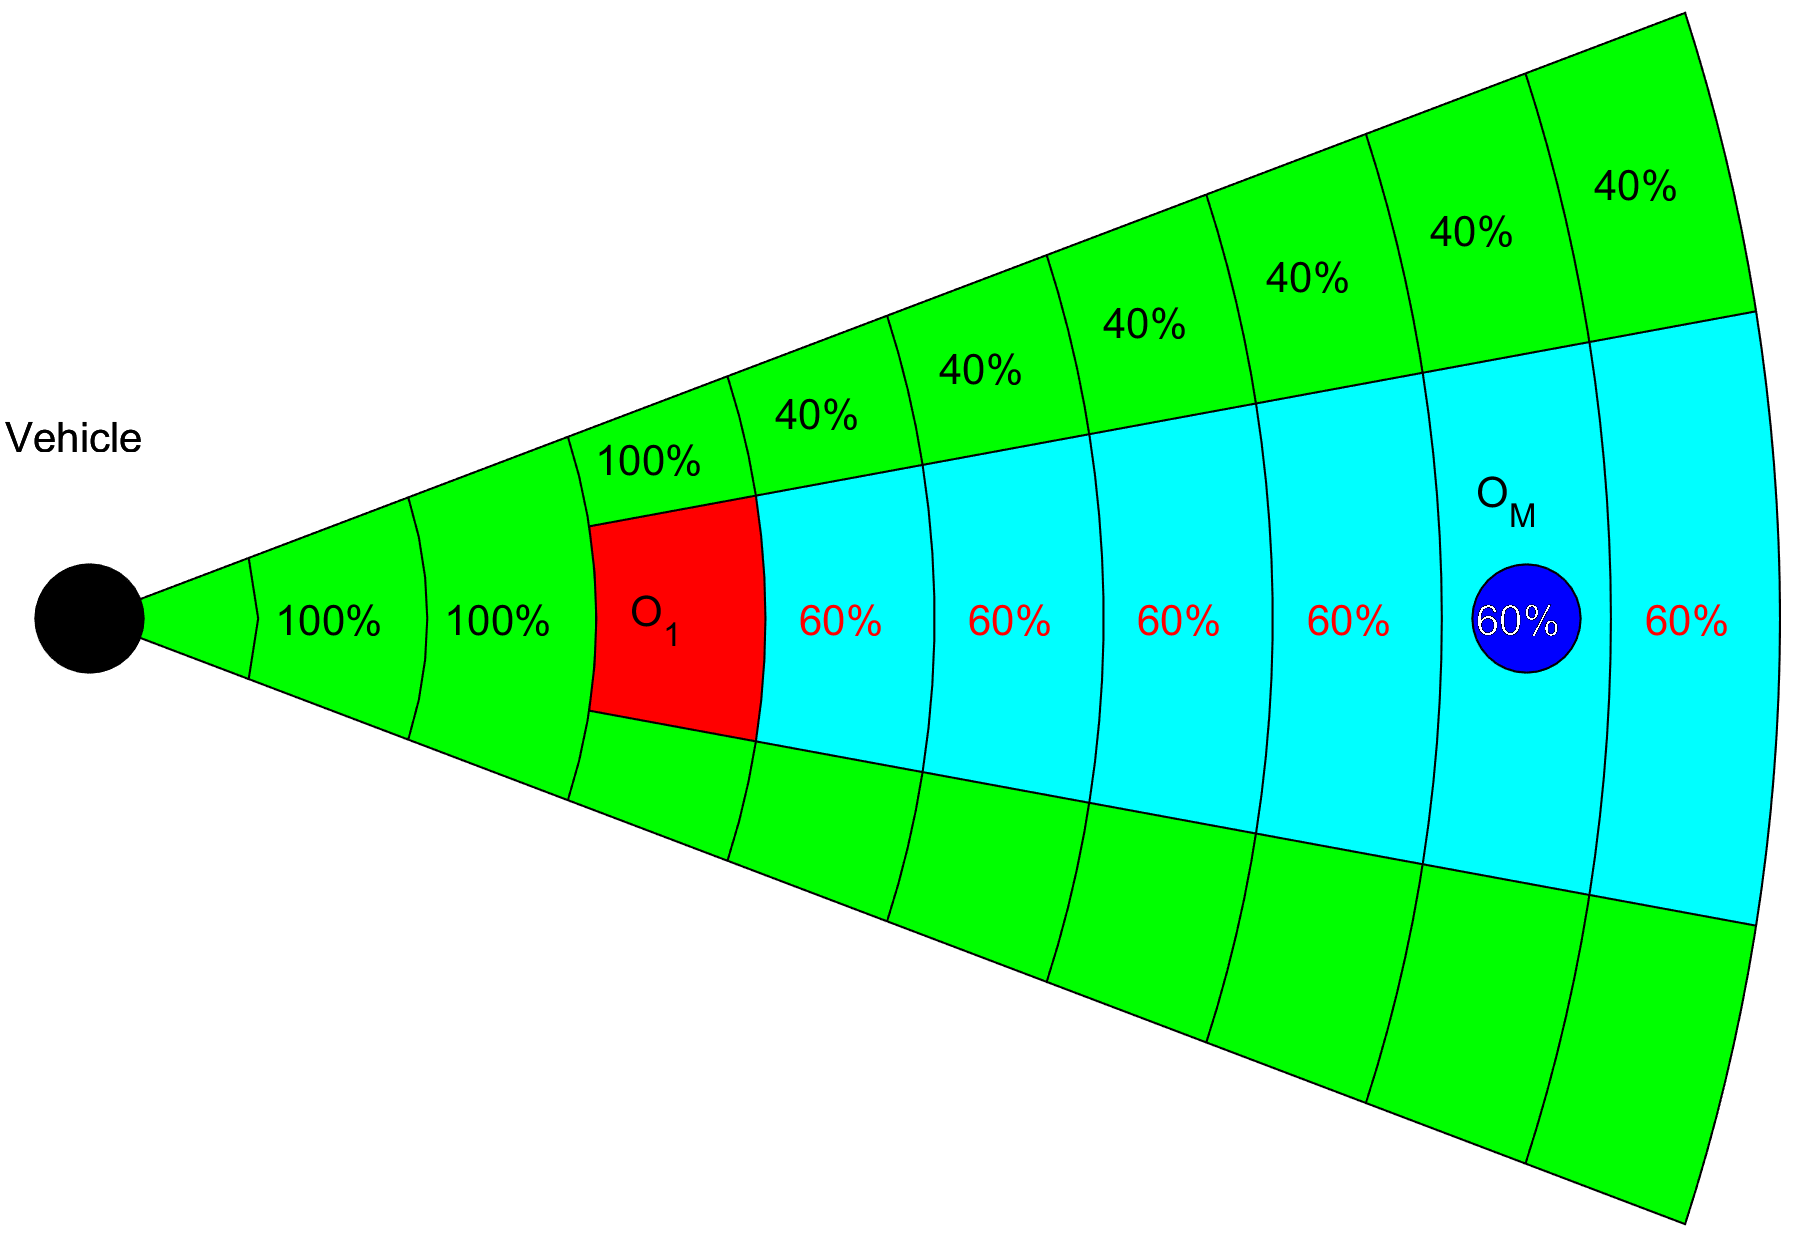
\includegraphics[width=0.7\textwidth]{\FIGDIR/P30MapObstacleHiden}
    \caption{Map obstacle - hidden behind detected obstacle}
    \label{fig:P30MapObstacleHiden}
\end{figure}

\noindent\emph{The formulation of final map obstacle probability} $P_{O_M}(c_{i,j,k})$ is given by previous examples which are giving the \emph{desired behaviour}. First we start with obstacle map definition.

The obstacle map $\mathscr{O}_m$ (\ref{eq:obstacleMap}) defines an map obstacle set $o=[\vec{p},\vec{o},r,\vec{a}]$ where $\vec{p}$ is position in global coordinate frame (center of mass), $\vec{o}$ is orientation bounded to global coordinate reference frame, $r$ is offset radius and $a$ is set pf additional parameters.
\begin{equation}\label{eq:obstacleMap}
    \mathscr{O}_M= \left\{[\vec{p},\vec{o},r,\vec{a}]:\vec{p}\in\R^3, \vec{o}\in\R^3, r\in (0,\infty),\vec{a}\in\R^k,k\in\N\right\}
\end{equation}

The space covered by any obstacle $o\to\R3$ is non-empty by definition. There are following types of charted obstacle considered in this example.

\begin{enumerate}
    \item\emph{Ball obstacle $\vec{a}=\varnothing$} - simple ball with center at $\vec{p}$, with offset radius $r$.
    \item\emph{Line obstacle $\vec{a}=[l]$} - simple line defined by length $l\in(0,\infty)$ with center at $\vec{p}$ and given orientation $\vec{o}$ with respect to main axis in global coordinate frame, with offset radius $r$.
    \item\emph{Plane obstacle $\vec{a}=[l,w]$} - bounded rectangle plane partition defined by length $l\in(0,\infty)$, and width $w\in(0,\infty)$ with center at $\vec{p}$ and given orientation $\vec{o}$ with respect to main axis in global coordinate frame, with offset radius $r$.
    \item\emph{Cuboid obstacle $\vec{a}=[l,w,d]$} - bounded cuboid space partition defined by length $l\in(0,\infty)$, width $w\in(0,\infty)$, and depth $d\in(0,\infty)$ with center at $\vec{p}$ and given orientation $\vec{o}$ with respect to main axis in global coordinate frame, with offset radius $r$.
\end{enumerate}
\noindent The obstacle set for some grid $\mathscr{A}$ at decision time $t_i$ intersection with obstacle map $\mathscr{O}_m$ is given by $\mathscr{O}_M(\mathscr{A}(t_i))$ (\ref{eq:obstacleMapAvoidanceGridIntersection}). Where map obstacle space $o$ is projected into avoidance grid space $\mathscr{A}(t_i)$. Projection output $\vec{p}_l\subset\R^3$ is partial subset of local coordinate frame space given by $A(t_i)$. If there exist non empty intersection between avoidance grid $\mathscr{A}(t_i)$ and local projection of obstacle space $\vec{p}_l$ then the given obstacle belongs to $\mathscr{O}_M(\mathscr{A}(t_i))$.

\begin{equation}\label{eq:obstacleMapAvoidanceGridIntersection}
    \mathscr{O}_M(\mathscr{A}(t_i))=\left\{o\in\mathscr{O}_M:\vec{p}_l:o \to\mathscr{A} (t_i), \vec{p}_l \cap \mathscr{A}(t_i)\neq\varnothing \right\}    
\end{equation}

\noindent $\mathscr{O}_M(c_{i,j,k},\mathscr{A}(t_i))$ (\ref{eq:obstacleMapCellSapceIntersection}) is analogy to $\mathscr{O}_M(\mathscr{A}(t_i))$ (\ref{eq:obstacleMapAvoidanceGridIntersection}). The cell space $c_{i,j,k}\subset\mathscr{A}(t_i)$ is considered as criterion instead of avoidance grid $\mathscr{A}(t_i)$. $\mathscr{O}_M(c_{i,j,k},\mathscr{A}(t_i))$ represents set of map obstacles in cell $c_{i,j,k}$ in context of acoidance grid $\mathscr{A}(t_i)$.

\begin{equation}\label{eq:obstacleMapCellSapceIntersection}
    \mathscr{O}_M(c_{i,j,k},\mathscr{A}(t_i))=\left\{o\in\mathscr{O}_M:\vec{p}_l:o \to\mathscr{A} (t_i), \vec{p}_l \cap c_{i,j,k} \neq \varnothing \right\}    
\end{equation}

\noindent\emph{Base probability of map obstacle} $P_{O_M,B}$ for single map obstacle $o\in\mathscr{O}_M$ (\ref{eq:baseProbabilityMapObstacleInCell}) is given as ration between intersection volume $\iiint (o\to\mathscr{A}(t_i))\cap c_{i,j,k} \quad \text{d}x\text{d}y\text{d}z$ and cell volume $\iiint c_{i,j,k}\quad\text{d}x\text{d}y\text{d}z$

\begin{equation}\label{eq:baseProbabilityMapObstacleInCell}
    P_{O_M,B}(o,c_{i,j,k}) = \frac{\iiint (o\to\mathscr{A}(t_i))\cap c_{i,j,k} \quad \text{d}x\text{d}y\text{d}z}{\iiint c_{i,j,k}\quad\text{d}x\text{d}y\text{d}z}
\end{equation}

\noindent\emph{Base probability of map obstacle} $P_{O_M,B}$ for map obstacle set  $\mathscr{O}_M$ (\ref{eq:baseProbabilityMapObstacleSetInCell}) is calculated in similar manner as base probability of map obstacle $P_{O_M,B}$ for single map obstacle $o\in\mathscr{O}_M$ (\ref{eq:baseProbabilityMapObstacleInCell}). The obstacle member of denominator has changed to space union of all obstacle space in local coordinate frame of avoidance grid $\mathscr{A}(t_i)$ as follow $\bigcup_{o\in\mathscr{O}_M}o\to\mathscr{A}(t_i)$.
\begin{equation}\label{eq:baseProbabilityMapObstacleSetInCell}
    P_{O_M,B}(\mathscr{O}_M,c_{i,j,k}) = \frac{\iiint \left(\bigcup_{o\in\mathscr{O}_M}o\to\mathscr{A}(t_i)\right) \cap c_{i,j,k} \quad \text{d}x\text{d}y\text{d}z}{\iiint c_{i,j,k}\quad\text{d}x\text{d}y\text{d}z}
\end{equation}

\noindent\emph{Final map obstacle probability} $P_{O_M}(c_{i,j,k})$ (\ref{eq:finalMapObstacleProbability}) is given as product of \emph{base probability of map obstacle} $P_{O_M,B}$ for map obstacle set  $\mathscr{O}_M$ (\ref{eq:baseProbabilityMapObstacleSetInCell}), and inverted \emph{final visibility probability $P_V(c_{i,j,k})$} (\ref{eq:FinalVisibilityProbability}). 
\begin{equation}\label{eq:finalMapObstacleProbability}
    P_{O_M}(c_{i,j,k})=P_{O_M,B}(\mathscr{O}_M,c_{i,j,k})\quad(\ref{eq:baseProbabilityMapObstacleSetInCell})\times\left(1-P_{V}(c_{i_c,j_c,k_c},\mathscr{S})\quad(\ref{eq:FinalVisibilityProbability})\right)
\end{equation}
\chapter{Simulation Results}\label{ch:06SimulationResults}
\section{Mission control}
\noindent This section briefly describes responsibilities and tasks of mission control module, implementation of mission control module is similar to \emph{LSTS-Neptus} \cite{dias2006mission,dias2005neptus}.

\paragraph{Navigation} main purpose is to execute mission between  ordered waypoint set $\mathscr{WP}$ (\ref{eq:waypointSet}). 

\begin{equation}\label{eq:waypointSet}
    \mathscr{WP}=\left\{W_1,W_2,\dots,W_n:W_i\in\R^3, i\in \left\{1,\dots,n\right\},n\ge 2\right\}
\end{equation}

\noindent Where each waypoint lies in 3D space $\R^3$ and there is at least two waypoints. There is enforcement of implementation condition that distance of any two consecutive waypoints $\forall i,j=i+1,\, \norm{W_i - W_j}\ge r_r$ is greater than reach radius $r_r$. \emph{Goal waypoint} $W_G$ is selected in following manner:
\begin{enumerate}
    \item\emph{First waypoint $W_1\in\mathscr{WP}$} is selected as goal waypoint $W_G$.
    \item\emph{Until last waypoint $W_n\in\mathscr{WP}$} is reached under reach condition $\norm{\vec{x}(t)\to\R^3-W_G}\le r_r$, check reach condition and select next waypoint in ordered set
    \item\emph{When last waypoint $W_n\in\mathscr{WP}$} is reached execute landing sequence. 
\end{enumerate}

\paragraph{Movement execution} of the movement automaton $\mathscr{MA}$ (def. \ref{def:movementAutomaton}). The main functionality of mission control is to link various movement buffers from avoidance grids $\mathscr{A}(t_i)$ into one single movement chain. The overall architecture has been presented in my earlier works \cite{alojzgomola2017}. 

The key concept is as follows. For dynamically generated set of decision times $t_1,$ $t_2,$ $\dots,$ $t_i$ there exists corresponding a set of avoidance grids $\mathscr{A}(t_1),\mathscr{A}(t_2),\dots,\mathscr{A}(t_i)$, where reach sets are given as set of trajectories. Each avoidance grid has corresponding avoidance trajectory which has been selected $\mathscr{T}(\vec{x},B)$. During a flight there exist a corresponding buffer for each decision time $t_1\to B_1, t_2 \to B_2,\dots,t_i\to B_i$. 

Single movement buffer $B_i$ from trajectory $\mathscr{T}(\hat{\vec{x})}(t_i),B_i)$ is given by following equation:
\begin{equation}
    B_i= \left\{m_{i,1},m_{i,2},\dots,m_{i,k},m_{i,k+1},\dots, m_{i,j-1},m_{i,j},\right\},\quad 1 \le k \le i, i \in \N^+
\end{equation}
Where $m_{i,1}$ is first \emph{to be executed/executed} and $m_{i,k}$ is last \emph{to be executed/executed} movement, $m_{i,k+1},\dots,m_{i,j}$ is flushed part (not used part of buffer), $k$ is count of \emph{to be executed/executed movements}, and $i$ is length of movement buffer $B_i$. This can be extended to any buffer belonging to any decision time. Then by assumptions given in \cite{alojzgomola2017}, there exists positive integer $k_i$ for any avoidance grid $\mathscr{A}(t_i)$ such movements can be chained.

\emph{Final movement buffer $B$} (\ref{eq:finalMovementBuffer}) is ordered chain of \emph{to be executed/executed} movements $\left\{m_{a,1},m_{a,2},\dots,m_{a,k}\right\}$ from partial trajectories at times of decision $t_{1},\dots,t_{i}$ with belonging buffers $\{B_1,\dots,B_i\}$.
\begin{equation}\label{eq:finalMovementBuffer}
    B=\bigcup_{B_a=\{B_1,\dots,B_i\}} \left\{m_{a,1},m_{a,2},\dots,m_{a,k}\right\}
\end{equation}
The example of \emph{final movement buffer $B$} is given in fig. \ref{fig:P46ExampleOfMovementBufferChaning}. The blue line represents \emph{to be executed/executed} movements, red line represents \emph{flushed movements}, purple circles represents \emph{decision points} at time $t_1,\dots,t_5$. Last portion at $t_5$ is denominated red, because it was completely throw away due the \emph{waypoint reach condition} was met.
\begin{figure}[H]
    \centering
    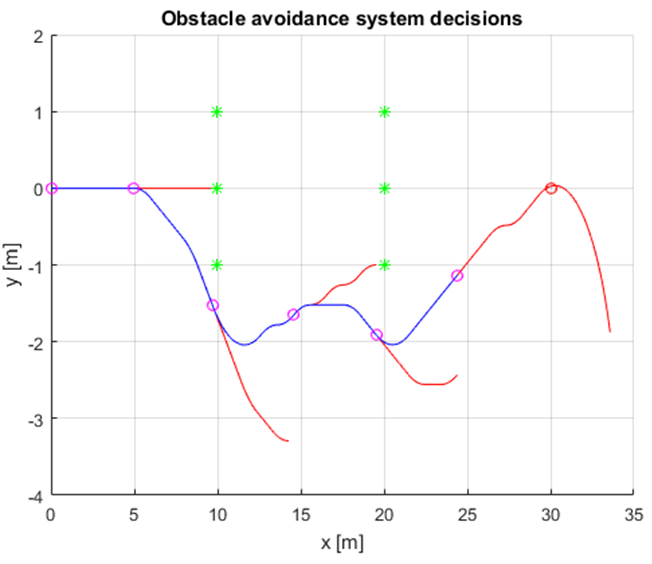
\includegraphics[width=0.7\textwidth]{\FIGDIR/P46ExampleOfMovementBufferChaning}
    \caption{Example of partial movement buffers chaining.}
    \label{fig:P46ExampleOfMovementBufferChaning}
\end{figure}

\paragraph{Obstacle processing and Control switch} has been reused from \cite{alojzgomola2017}.

\section{Reduced reach set approximation computation}
\noindent The worst case scenario for LiDAR scanning have been given in \cite{sabatini2014lidar}. That means the minimal conical range of LiDAR in middle class is $\tilde10$ $m$. The main idea is to test spread reduction vs. coverage ratio $C_R$ on grid with many layers. The deterministic approach of reach set estimation in \cite{alojzgomola2017} was sustainable to calculate full reach set for 5 movements and 10 layers, that implies count of nodes ($n=\sum_{i=1}^10 5^i$). The proposed grid will have 15 layers and 9 movements (estimation of such reach set in full form is impossible). \emph{The pruning of unfeasible pathways} is executed in iterative manner, which enables to minimize memory consumption and effort during \emph{reach set estimation calculation}. The scalability of presented approaches is one of the main features and even the calculation time is scaling well. The approximation algorithm implementation has \emph{borderline polynomial} complexity.


Three different methods have been developed and tested on following avoidance grid $\mathscr{A}(t_i)$:
\begin{enumerate}
    \item Range = 15m, 15 layers
    \item Horizontal range: $\theta\in[-\frac{\pi}{4};\frac{\pi}{4}]$, 7 horizontal cells
    \item Vertical range: $\varphi\in[-\frac{\pi}{6};\frac{\pi}{6}]$, 5 vertical cells
    \item 525 cells, 35 for each layer
\end{enumerate}

\emph{Complexity} of unbounded tree search with pruning procedure after computation is given as:
\begin{equation}
    \mathscr{O}(n) \le m \times r\times h\times v\times l + e^{m \times r} 
\end{equation}
Where $m$ - is count of movements, $r$ is spread rating, $h$ is horizontal cell count of $\mathscr{A}(t_i)$, $v$ is vertical cell count of $\mathscr{A}(t_i)$, $l$ is layer count of $\mathscr{A}(t_i)$. The problematic term is $e^{m \times r}$ which is exponential unexplored nodes residuum. The complexity $\mathscr{O}(n)$ is non-polynomial now. 

To solve this issue the post-expansion pruning algorithm needs to be introduced, this allows to transform $e^{m \times r}$ to a linear/polynomial member $m  \times h \times v \times l$. Therefore complexity $\mathscr{O}(n)$ is now bounded by: 
\begin{equation}
    \mathscr{O}(n) \le m\times (r+1)\times h\times v\times l
\end{equation}
The spread ratio $r$ and movement count $h$ is given, the scalable parameters are grid member counts $h,v,l$, it is obvious that $h\times v \times  l$ is cell count $|\mathscr{A}(t_i)|$. For our grid following formula for boundary can be used:
\begin{equation}
    \mathscr{O}(n) \le 9\times k \times 525
\end{equation}

\noindent The performance parameters for various algorithms are summarized in following table:
\begin{table}[H]
    \centering
    \begin{tabularx}{\textwidth}{l||cccX}
    
    Method/Parameter & Nodes & Trajectories & Coverage ratio $C_R$ & Note\\\hline\hline
    Chaotic method& 2483 & 725 & 0.90 & Forced spread: 9\\
    Harmonic method& 1405 & 180 & 0.30 & \\
    Combined method& 2162 & 305 & 0.87 & CH: 8, H: 1\\
    \end{tabularx} 
    \caption{Reduced reach set computation methods performance}
    \label{tab:RRMethodsPerformanceComparison}
\end{table}

\noindent Reduced reach set approximation $\mathscr{R}_R$ using combined method can cover almost same cell footprints with very small node count:
\begin{equation}
    \frac{\text{node count } \mathscr{R}_R}{\text{node count } \mathscr{R}_F} = \frac{2483}{\sum_{k=1}^{15} 9^k}\sim 1.2088 \times 10^{-12}
\end{equation}
\noindent Depending on selected spread algorithm and pruning algorithm, the reduced reach set keep properties:
\begin{enumerate}
    \item \textit{Smoothness} - trajectories contained in reduced reach set approximation are smooth and with low cost.
    \item \textit{Coverage $C_\mathscr{R}$} - trajectories are covering high amount of footprints from full reach set approximation footprint set $\mathscr{Q}_F$.
\end{enumerate}


\section{Moving obstacles spread models}
\noindent This section discuss implementation and performance of various intruder intersection models. The conditions of intersection was stated as continuous space problem,for real implementation numeric approximation methods keeping probabilistic properties of continuous space were used. 
\noindent Following basic models have been identified in section \ref{sec:intruderIntersectionModel}.:
\begin{enumerate}
    \item \textit{Direct (Line) Intersection} - for static/timed environment.
    \item \textit{Future (Line) Movement} -  for timed environment.
    \item \textit{Vehicle body volume} -  for timed environment.
    \item \textit{Uncertainty spread} -  for static/timed environment.
\end{enumerate}
\noindent Given is intruder $I$ with following properties:
\begin{enumerate}
    \item\textit{Position in Local Coordinate Frame} -  $[6,8,0]^T$
    \item\textit{Velocity} - scalar $1ms^{-1}$, vector $[0,-1,0]^T \quad [ms^{-1},ms^{-1},ms^{-1}]$
    \item\textit{Horizontal spread $\theta$} - $[-\pi/12,\pi/12]\quad [rad,rad]$
    \item\textit{Vehicle body radius} - $2 m$
    \item\textit{Vertical spread $\varphi$} - $[-\pi/16,\pi/16]\quad [rad,rad]$
\end{enumerate}

\noindent All intersection methods have been tested on following avoidance grid $\mathscr{A}(t_i)$:
\begin{enumerate}
    \item Range = 10 m, 10 layers
    \item Horizontal range: $\theta\in[-\frac{\pi}{4};\frac{\pi}{4}]$, 7 horizontal cells
    \item Vertical range: $\varphi\in[-\frac{\pi}{6};\frac{\pi}{6}]$, 5 vertical cells
    \item 350 cells, 35 for each layer
\end{enumerate}

\subsection{Line intersection - Static}
\noindent For line intersection standard \emph{line back-stepping} numeric algorithm was used. Base intersection probability for line $P_T(i_k(\vec{x},\vec{v}),c_{i,j,k})$  (\ref{eq:baseIntersectionProbabilityLineIntersectionType}) was used. The implementation is trivial and intersection probability $P_{O_I}(i_k,c_{i,j,k},l,b,s,\tau)$ (\ref{eq:intruderInCellProbabilityOneIntruder}) The flags are set $l=1$, $b=0$, $s=0$, and $\tau=0$. That means only line intersection is accounted. 
\begin{figure}[H]
    \centering
    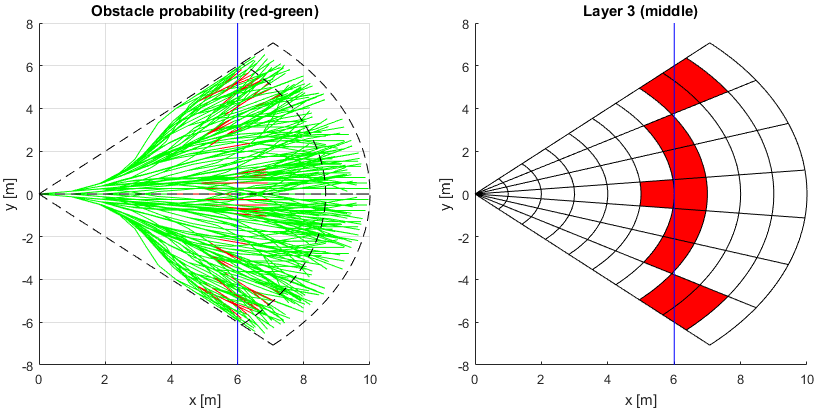
\includegraphics[width=0.7\textwidth]{\FIGDIR/P08LineStaticObstacleSpace}
    \caption{Obstacle space for static line intersection}
    \label{fig:P08LineStaticObstacleSpace}
\end{figure}
\noindent The figure \ref{fig:P08LineStaticObstacleSpace} is showing trajectory space and middle horizontal layer obstacle space $\mathscr{O}(t)$. The blue line is representing intruder intersection trajectory starting at top and finishing at bottom of avoidance grid $\mathscr{A}(t_i)$. The red portion of trajectories on left sub-figure is reflecting the impacted portions of UAV trajectories. The red cells on right sub-figure are reflecting impacted cells with probability of intruder $P_I=1$.
\begin{figure}[H]
    \centering
    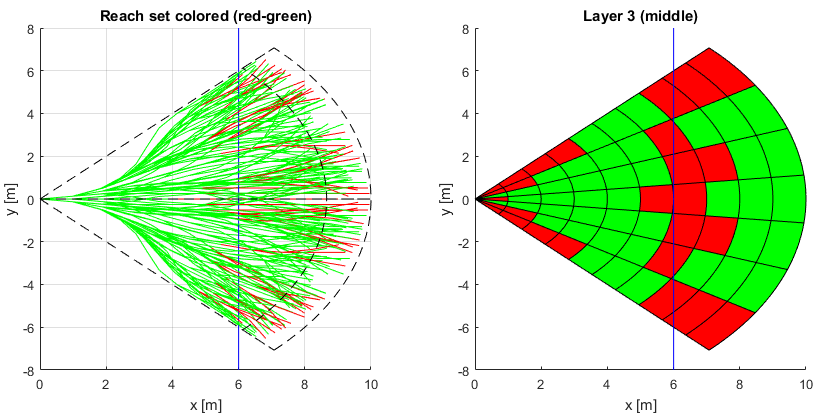
\includegraphics[width=0.7\textwidth]{\FIGDIR/P09LineStaticReachSet}
    \caption{Reach set approximation for static line intersection - middle layer}
    \label{fig:P09LineStaticReachSet}
\end{figure}

\noindent The figure \ref{fig:P09LineStaticReachSet} is showing reachable set approximation trajectories $\mathscr{R}(\hat{x}(t_i),t_i,t_{i+1})$ and middle layer of avoidance grid $\mathscr{A}(t_i)$ with assessed reachability. The blue line is denominating the intruder trajectory (side approach), it starts at top and ends at bottom. The left sub-figure shows set of trajectories where green parts are executable and red parts are crash trajectories. The right sub-figure shows the \emph{reachable space}, the red cells are cells which can not be reached and the green cells are cells which can be reached. Notice that the green cells in front are reachable, because there exists at least one trajectory leading there trough unoccupied space. 

\subsection{Line intersection - Timed}
\noindent For line intersection standard \emph{line back-stepping} numeric algorithm was used. Base intersection probability for line $P_T(i_k(\vec{x},\vec{v}),c_{i,j,k})$  (\ref{eq:baseIntersectionProbabilityLineIntersectionType}) was used. The implementation is trivial and intersection probability $P_{O_I}(i_k,c_{i,j,k},l,b,s,\tau)$ (\ref{eq:intruderInCellProbabilityOneIntruder}) The flags are set $l=1$, $b=0$, $s=0$, and $\tau=1$. That means The base intersection probability and time interval intersection probability components are accounted. The expected danger zones are valid if and only if the intruder and vehicle velocity remains constant. If this condition can not be full-filled the $\tau=0$ in probabilistic model. The obstacle probability is denoted in white/red scale, the reachability probability is denoted in green/red scale.

\begin{figure}[H]
    \centering
    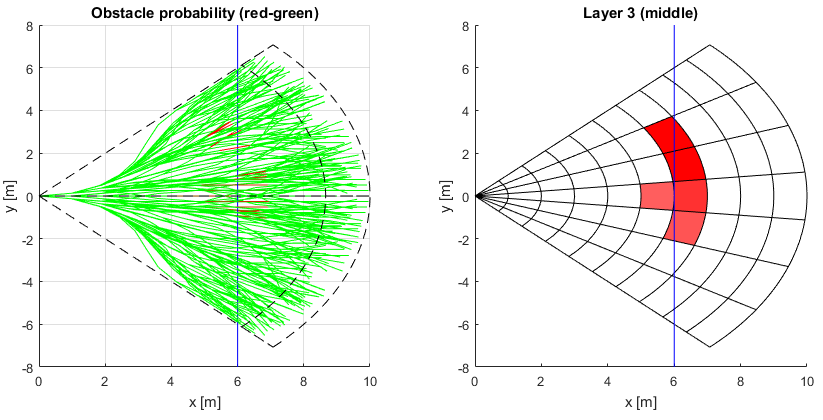
\includegraphics[width=0.7\textwidth]{\FIGDIR/P10LineTimedObstacleSpace}
    \caption{Obstacle space for timed line intersection}
    \label{fig:P10LineTimedObstacleSpace}
\end{figure}

\noindent The figure \ref{fig:P10LineTimedObstacleSpace} is showing trajectory space and middle horizontal layer obstacle space $\mathscr{O}(t)$. The blue line is representing intruder intersection trajectory starting at top and finishing at bottom of avoidance grid $\mathscr{A}(t_i)$. The red portion of trajectories on left sub-figure is reflecting the impacted portions of UAV trajectories. The red cells on right sub-figure are reflecting impacted cells with probability of intruder $P_I\in [0,1]$. Notice that probability of intersection is not always equal to 1, because of time component it can be slightly decreased (pink cells).

\begin{figure}[H]
    \centering
    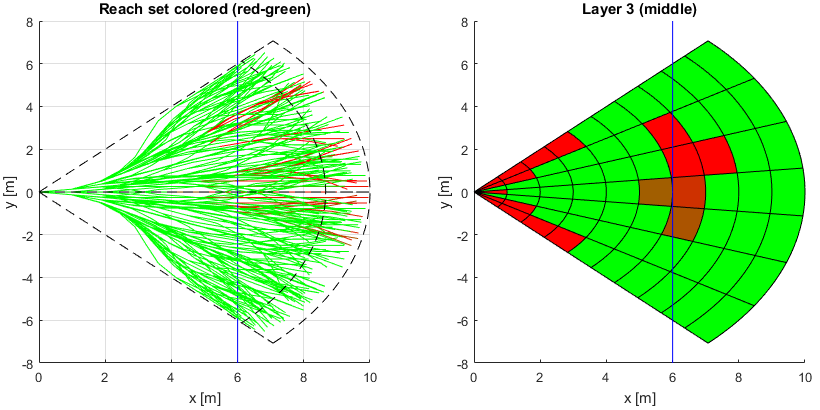
\includegraphics[width=0.7\textwidth]{\FIGDIR/P11LineTimedReachSet}
    \caption{Reach set approximation for timed line intersection - middle layer}
    \label{fig:P11LineTimedReachSet}
\end{figure}


\noindent The figure \ref{fig:P11LineTimedReachSet} shows reachability property intersection with intruder linear trajectory (light blue). The left sub-figure shows the approximation of reach set $\mathscr{R}(\hat{x}(t_i),t_i,t_{i+1})$. The set of trajectories is colored in green-red color, meaning that reachability of the trajectory is absolute when green or not reachable at all if red. The left sub-figure shows reachability status of cells in middle layer. Some of cells are unreachable with reachability probability $P_R(c_{i,j,k})\in [0,1)$. Please note that last layer is fully reachable and intruder can be avoided via the other layers.

\subsection{Line intersection - Future movements}
\noindent For line intersection standard \emph{line back-stepping} numeric algorithm was used. Base intersection probability for line $P_T(i_k(\vec{x},\vec{v}),c_{i,j,k})$  (\ref{eq:baseIntersectionProbabilityLineIntersectionType}) was used. The implementation is trivial and intersection probability $P_{O_I}(i_k,c_{i,j,k},l,b,s,\tau)$ (\ref{eq:intruderInCellProbabilityOneIntruder}) The flags are set $l=1$, $b=0$, $s=0$, and $\tau=1$. That means The base intersection probability and time interval intersection probability components are accounted. The expected danger zones are valid if and only if the intruder and vehicle velocity remains constant. If this condition can not be full-filled the $\tau=0$ in probabilistic model. The obstacle probability is denoted in white/red scale, the reachability probability is denoted in green/red scale. There has been implemented a special case for future movement and it improves time intersection probability:
\begin{equation}
    P_{O_I}(i_k,c_{i,j,k})=
    \begin{cases}
    t_e\ge i_l :& P_{O_I}(i_k,c_{i,j,k},l=1,b=0,s=0,\tau=1)\\
    t_e < i_l  :& P_{O_I}(i_k,c_{i,j,k},l=1,b=0,s=0,\tau=0)/2\\
    \end{cases}
\end{equation}
\noindent Where $t_e$ is vehicle entry time to cell $c_{i,j,k}$, $i_l$ is intruder leave time of cell $c_{i,j,k}$ other notation strictly follows (\ref{eq:intruderInCellProbabilityOneIntruder}). The main idea is to force avoidance from behind of intruder heading, which has been achieved, but is not required to encode higher level decision logic into probabilistic distributions.


\begin{figure}[H]
    \centering
    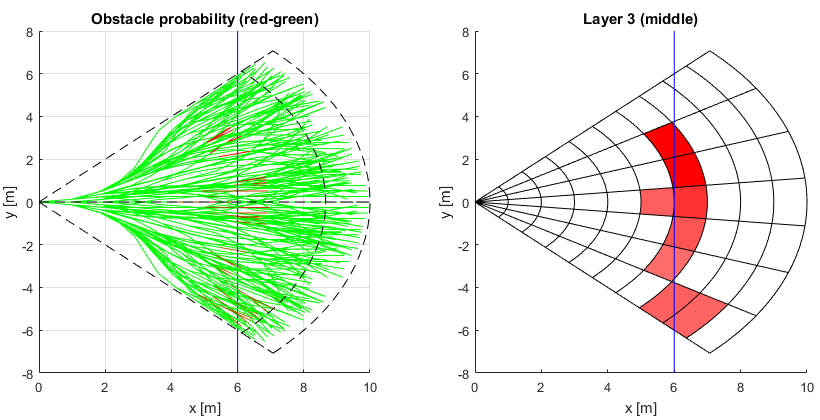
\includegraphics[width=0.7\textwidth]{\FIGDIR/P12LineFutureObstacleSpace}
    \caption{Obstacle space for timed line intersection with future movement}
    \label{fig:P12LineFutureObstacleSpace}
\end{figure}


\noindent The figure \ref{fig:P12LineFutureObstacleSpace} is showing trajectory space and middle horizontal layer obstacle space $\mathscr{O}(t)$. The blue line is representing intruder intersection trajectory starting at top and finishing at bottom of avoidance grid $\mathscr{A}(t_i)$. The red portion of trajectories on left sub-figure is reflecting the impacted portions of UAV trajectories. The red cells on right sub-figure are reflecting impacted cells with probability of intruder $P_I\in [0,1]$. Notice that probability of intersection is not always equal to 1, because of time component it can be slightly decreased (pink cells). The future movement cells are located as new addition at bottom of trajectory, for reference compare fig. \ref{fig:P10LineTimedObstacleSpace}.

\begin{figure}[H]
    \centering
    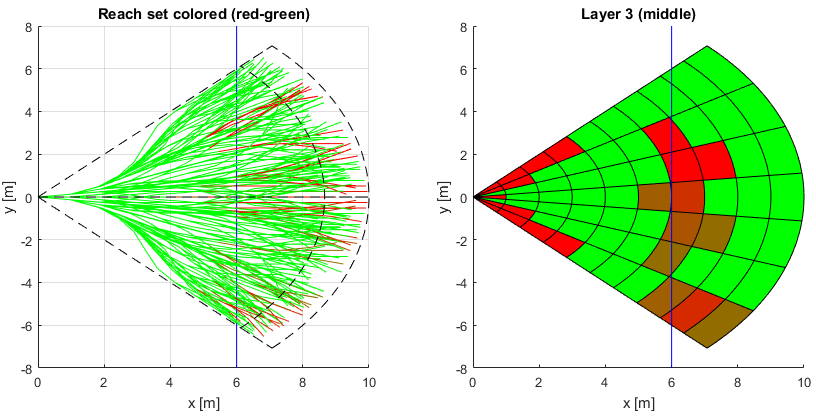
\includegraphics[width=0.7\textwidth]{\FIGDIR/P13LineFutureReachableSpace}
    \caption{Reach set approximation for timed line intersection with future movement - middle layer}
    \label{fig:P13LineFutureReachableSpace}
\end{figure}

\noindent The figure \ref{fig:P13LineFutureReachableSpace} shows reachability property intersection with intruder linear trajectory (light blue). The left sub-figure shows the approximation of reach set $\mathscr{R}(\hat{x}(t_i),t_i,t_{i+1})$. The set of trajectories is colored in green-red color, meaning that reachability of the trajectory is absolute when green or not reachable at all if red. The left sub-figure shows reachability status of cells in middle layer. Some of cells are unreachable with reachability probability $P_R(c_{i,j,k})\in [0,1)$. Please note how reach set have been changed due the future movements, it is almost certain that vehicle will avoid intruder from behind (fig. \ref{fig:P11LineTimedReachSet}).


\subsection{Vehicle body volume - timed}
\noindent\emph{Base intersection probability} $P_T(i_k(\vec{x},\vec{v},r),c_{i,j,k})$ (\ref{eq:baseIntersectionProbabilityBallIntersectionType}) is defined for volume ball $\mathscr{B}(\vec{x}(t),r)$ (\ref{eq:volumeballofIntruder}). The volume ball 
$\mathscr{B}(\vec{x}(t),r)$ is given only as a boundary can be represented as a convex set $S_1$. The grid cell $c_{i,j,k}$ can be represented as polyhedron. The numeric approximation of these two structures intersection was proposed in \cite{deutsch1999best}, \emph{strong conical hull intersection property} guarantees to avoid false positive intersection cases. The algorithm in \cite{deutsch1999best} also gives the volume of the output, which can be used to enhance  \emph{base intersection probability} like follow:

\begin{equation}
    P_T(i_k(\vec{x},\vec{v},r),c_{i,j,k},t)= \frac{V(c_{i,j,k}\cap \mathscr{B}(\vec{x}(t),r))}{V(c_{i,j,k})} \in [0,1]
\end{equation}

\noindent Where $V(c_{i,j,k}\cap \mathscr{B}(\vec{x}(t),r))$ is volume of cell $c_{i,j,k}$ belonging to some avoidance grid $\mathscr{A}(t_i)$ at some avoidance time $t_i$, intersected with a volume of ball $\mathscr{B}$ with center given by $\vec{x}(t)$ (\ref{eq:intruderBasicLinearModel}) and radius $r$. The denominator is simple volume of cell $V(c_{i,j,k})$. The volume of convex polytopes can be calculated with linear complexity $\mathscr{O}(n)$, where $n$ is count of vertexes as proposed in \cite{lawrence1991polytope}.

This is great for fixed time $t$, but the time is not fixed in our case. For fixed time interval $[t_e,t_l]$ where $t_e$ entry time is given as first time when $P_T(i_k(\vec{x},\vec{v},r,t),c_{i,j,k})\neq 0$, and $t_l$ leave time is given as the last time when $P_T(i_k(\vec{x},\vec{v},r,t),c_{i,j,k}) \neq 0$. Then base probability $P_T(i_k(\vec{x},\vec{v},r),c_{i,j,k})$ for varying time $t \in [t_e,t_l]$ can be obtained as a maximum of all probable intersections $P_T(i_k(\vec{x},\vec{v},r),c_{i,j,k},t)$, summarized in following equation:

\begin{equation}
    P_T(i_k(\vec{x},\vec{v},r),c_{i,j,k}) = \max_{t\in [t_e,t_l]} P_T(i_k(\vec{x},\vec{v},r),c_{i,j,k},t)
\end{equation}

\noindent\emph{Tubular intersection} is possible low-cost replacement for embedded, systems, this type of intersection is similar to \emph{conic intersection} (\ref{eq:conicIntersectionCellIntruderDiscrete}), but the vehicle body radius parameter $r_b$ is independent on time. The tubular slice is given as follow: 
\begin{equation}
    \mathscr{T}(\vec{x}(t),\vec{v},r_s,r_b)=\left\{\vec{p}\in\R^3:\forall_{i\neq j} p_i \exists p_j, ||p_i-p_j|| \le r_s, \left(\vec{p} -\vec{x}\right)\perp \vec{v},  \norm{\vec{p}-\vec{x}}\le r_b\right\}
\end{equation}
\noindent\emph{Tubular slice} fox fixed time $t$ and given vehicle position $\vec{x}(t)\in\R^3$ and orientation $\vec{v}\in\R^3$ with defined step radius $r_s$ and defined body radius $r_r$ is given as set of points where each point holds following up to following conditions:
\begin{enumerate}
    \item $\forall_{i\neq j} p_i \exists p_j, ||p_i-p_j|| \le r_s$ - for each point $p_i$ there exists a point $p_j(i \neq j)$ within the step radius $r_s$. This guarantees coverage and homogeneity, the $r_s$ is chosen as 1/10 of average cell $c_{i,j,i,k}\in\mathscr{A}(t_i)$ radius.
    \item $\left(\vec{p} -\vec{x}\right)\perp \vec{v}$ - all points $\vec{p}$ are orthogonal  to velocity vector $\vec{v}$.
    \item $\norm{\vec{p}-\vec{x}}\le r_b$ - all points are within bounded area of circle given by body radius $r_b$.
\end{enumerate}
\noindent The \emph{tube approximation} is given by following equation:
\begin{equation}
    \mathscr{T}(\vec{x},\vec{v},r_s,r_b) = \left\{\bigcup_{\vec{x}(t)=f(\vec{x},\vec{v})}^{t\in[t_s,t_e]} \mathscr{T}(\vec{x}(t),\vec{v},r_s,r_b)\right\}
\end{equation}
\noindent The \emph{tube approximation} is simply union of all tubular slices over defined time period $[t_e,t_l]$ where $t_e$ is entry time and $t_l$ is leave time, mentioned earlier. The interval can be discredited by using steepest function or simple marginalization rule $\norm{\vec{x}(t_i) - \vec{x}(t_{i+1})} \le r_r$. 

If \emph{tube approximation} is used the cell entry $t_e(c_{i,j,k})$ and leave time $t_l(c_{i,j,k})$ are given based on \emph{tubular slices} intersection $\mathscr{T}(\vec{x}(t),\vec{v},r_s,r_b)$ time $t$.

\begin{figure}[H]
    \centering
    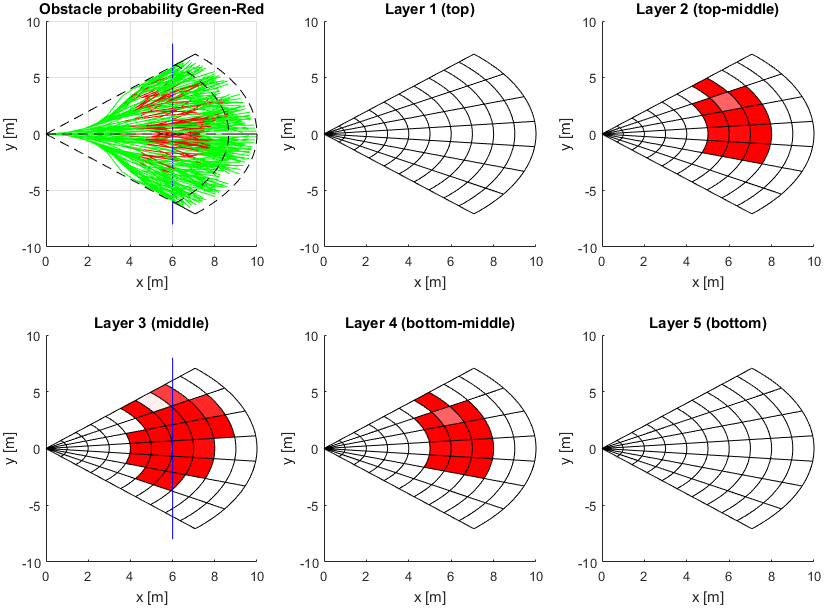
\includegraphics[width=\textwidth]{\FIGDIR/P14VolumeTimedObstacleSpace}
    \caption{Obstacle space for timed intruder body volume}
    \label{fig:P14VolumeTimedObstacleSpace}
\end{figure}
\emph{Obstacle space} for \emph{intruder body volume} with time dependency is depicted in fig. \ref{fig:P14VolumeTimedObstacleSpace} with following meaning:
\begin{enumerate}
    \item\emph{Obstacle probability} - shows how three consequent timed balls $\mathscr{B}(\vec{x}(t),r=1)$ are projected intro reach set approximation $\mathscr{R}(\hat{x}(t_i),t_i,t_{i+1})$, red denotes unfeasible part of trajectories crossing dangerous area where intruder body can be encountered
    \item\emph{Layer 1 (top)} - shows that there is any expectation of intruder body.
    \item\emph{Layer 2} - contains top part of ball intersections, shades of red are denoting intersection probability $[0,1]$, $[white,red]$.
    \item\emph{Layer 3 (middle)} - contains middle part of ball intersections, shades of red are denoting intersection probability $[0,1]$, $[white,red]$. The blue line denotes intruder linear trajectory. 
    \item\emph{Layer 4} - contains bottom part of ball intersections, shades of red are denoting intersection probability $[0,1]$, $[white,red]$.
    \item\emph{Layer 5 (bottom)} - shows that there is any expectation of intruder body.
\end{enumerate}

\begin{figure}[H]
    \centering
    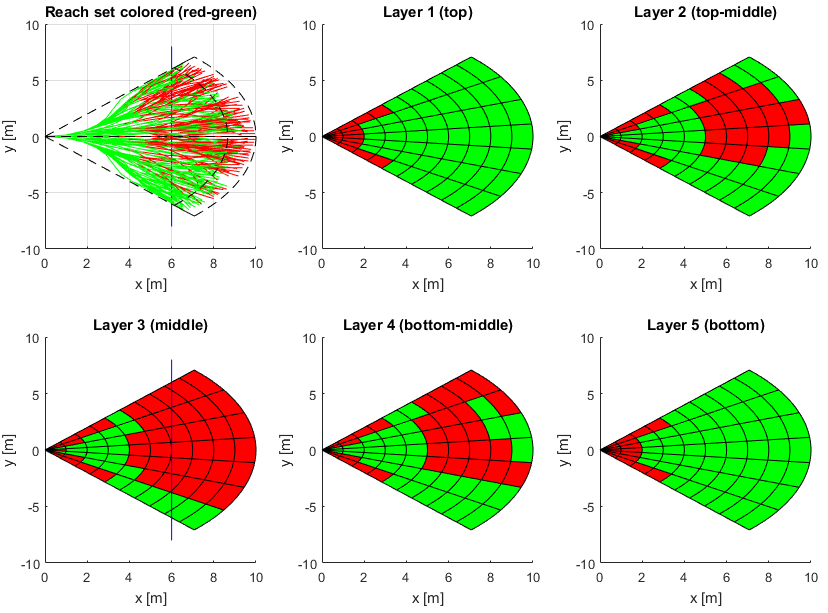
\includegraphics[width=\textwidth]{\FIGDIR/P15VolumeTimedReachSet}
    \caption{Reach set approximation for timed vehicle body volume - all layers}
    \label{fig:P15VolumeTimedReachSet}
\end{figure}

\noindent\emph{Reach set approximation for timed vehicle body volume}  is given by fig. \ref{fig:P15VolumeTimedReachSet}, the explanation of figure is following:
\begin{enumerate}
    \item\emph{Reachability probability} (red-green scale) shows reachability of each point of trajectories contained in reach set approximation $\mathscr{R}(\hat{x}(t_i),t_i,t_{i+1})$, the red shades denotes unreachable parts of trajectories and the green part denotes reachable parts of trajectories.
    \item\emph{Layer 1 (top)} - the top layer is completely reachable.
    \item\emph{Layer 2} - the portion of layer is unreachable, note that some frontal cells are reachable, because there exists trajectories from first layer.
    \item\emph{Layer 3 (middle)} - the middle layer is almost completely unreachable due the intruder occupation of neighbouring layers, intruder trajectory is denoted by blue line.
    \item\emph{Layer 4} - the portion of layer is unreachable due the vehicle body, note that some frontal cells are reachable due the existence of trajectories leading trough fith layer. 
    \item\emph{Layer 5 (bottom)} - the bottom layer is completely reachable
\end{enumerate}

\subsection{Uncertainty spread - Static}
\noindent\emph{Intruder linear model} $\vec{x}(t)=f(\vec{x},\vec{v})$ have been introduced by \ref{eq:vehiclelinearcone}, its simple linear trajectory model, base intersection structure is  \emph{ellipsoid} $E(\vec{x}(t),\vec{v})$ (\ref{eq:baseElipsoidxt}). The \emph{base intersection probability} for single intruder $i_k$ defined as $P_T(i_k(\vec{x}_s,\vec{v},\theta,\varphi),c_{i,j,k})$ is given by \ref{eq:spreadIntruderIntersectionProbDiscrete}. Intruders $i_k$ intersection times for single cell $c_{i,j,k}\in\mathscr{A}(t_i)$ are defined as follow:
\begin{enumerate}
    \item\emph{Intruder time of entry} $i_e(i_k,c_{i,j,k})$ (\ref{eq:conicTimeOfEntryDiscrete}).
    \item\emph{Intruder time of leave} $i_l(i_k,c_{i,j,k})$ (\ref{eq:conicTimeOfLeaveDiscrete}).
\end{enumerate}
\emph{Single Intruder intersection model} $ P_{O_I}(i_k,c_{i,j,k},l,b,s,\tau)$ (\ref{eq:intruderInCellProbabilityOneIntruder}) set up with following flags:  spread flag $s=1$. Because the conical intersection covers a huge amount of space in avoidance grid $\mathscr{A}(t_i)$ it is recommended not to overshoot intruder \emph{horizontal spread} $\theta$ and intruder \emph{vertical spread} $\varphi$ estimates.

\emph{Intruder obstacle probability} $P_{O_I}(c_{i,j,k})$ (\ref{eq:intruderInCellProbability}) was not considered in this simulation, because single intruder was used.  Overall implementation is straightforward transcription of mentioned definitions. 
\begin{figure}[H]
    \centering
    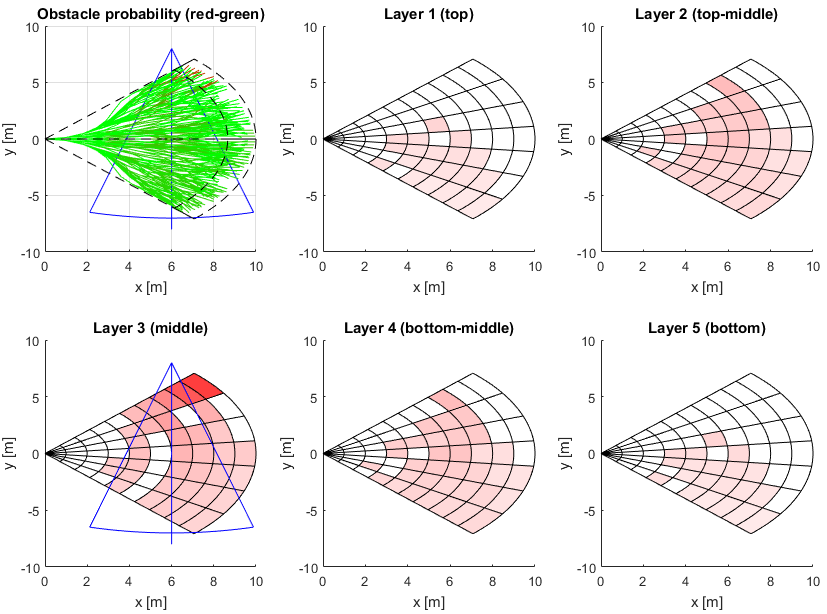
\includegraphics[width=\textwidth]{\FIGDIR/P16SpreadStaticObstacleSpace}
    \caption{Obstacle space for static uncertainty spread}
    \label{fig:P16SpreadStaticObstacleSpace}
\end{figure}

\noindent Uncertainty cone intersection is creating \emph{virtual obstacles}, because real obstacle is moving intruder body. The cone is denoted as \emph{blue} line borders, with notion of vehicle linear trajectory (center axis of cone). Obstacle probability is more concentrated at the detection point (upper part of diagrams) and becomes more spread and thin with increasing horizontal $\theta$ and horizontal $\varphi$ spread. The intruder clash (obstacle) probability distribution is in fig. \ref{fig:P16SpreadStaticObstacleSpace} with following sub-figures:
\begin{enumerate}
    \item\emph{Obstacle probability} - displays impact of intruder on trajectory parts where the intersection with intruder is probable, green denotes low probability, red denotes high probability. The probability is fairly (slightly brownish) low, because of wide spread of intruder horizontal $\theta$, and vertical $\varphi$ distributions.
    \item\emph{Layer 1 (top)} - there is only residual clash probability at the bottom of the diagram, due high vertical spread $\varphi$ value.
    \item\emph{Layer 2} - there is more residual clash probability at the bottom of the diagram, due high vertical spread $\varphi$ value.
    \item\emph{Layer 3 (middle)} - cash probability is concentrated at the top and slowly vanishes over distance from point of detection, due the high horizontal spread $\theta$ value.
    \item\emph{Layer 4} - there is more residual clash probability at the bottom of the diagram, due high vertical spread $\varphi$ value.
    \item\emph{Layer 5 (bottom)} - there is only residual clash probability at the bottom of the diagram, due high vertical spread $\varphi$ value.
\end{enumerate}


\begin{figure}[H]
    \centering
    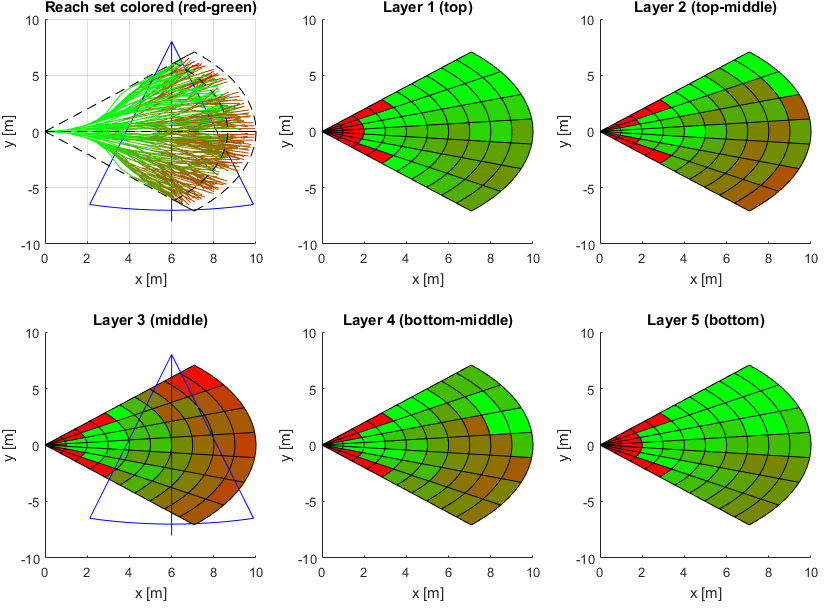
\includegraphics[width=\textwidth]{\FIGDIR/P17SpreadStaticReachSet}
    \caption{Reach set approximation for static uncertainty spread - all layers}
    \label{fig:P17SpreadStaticReachSet}
\end{figure}

\noindent Reach set $\mathscr{R}(\hat{x},t_i,t_{i+1})$(fig. \ref{fig:P17SpreadStaticReachSet}) is given as follow:
\begin{enumerate}
    \item\emph{Reachibility probability} - The reachability probability of trajectories reflects obstacle set $\mathscr{O}(t_i)$
    \item\emph{Layer 1 (top)} - the residual obstacle probability caused from extreme values of \emph{vertical spread} $\varphi$ are causing lowered reachability in lower portions of cells. The upper part is relatively safe.
    \item\emph{Layer 2} - the residual obstacle probability caused from extreme values of \emph{vertical spread} $\varphi$ are causing significantly lowered reachability in lower portions of cells. The upper part is still safe.
    \item\emph{Layer 3 (middle)} - reflects the middle layer in fig. \ref{fig:P16SpreadStaticObstacleSpace}. 
    \item\emph{Layer 4} - the residual obstacle probability caused from extreme values of \emph{vertical spread} $\varphi$ are causing significantly lowered reachability in lower portions of cells. The upper part is still safe.
    \item\emph{Layer 5 (bottom)} - the residual obstacle probability caused from extreme values of \emph{vertical spread} $\varphi$ are causing lowered reachability in lower portions of cells. The upper part is relatively safe.
\end{enumerate}


\subsection{Uncertainty spread - Timed}
\noindent\emph{Intruder linear model} $\vec{x}(t)=f(\vec{x},\vec{v})$ have been introduced by \ref{eq:vehiclelinearcone}, its simple linear trajectory model, base intersection structure is  \emph{ellipsoid} $E(\vec{x}(t),\vec{v})$ (\ref{eq:baseElipsoidxt}). The \emph{base intersection probability} for single intruder $i_k$ defined as $P_T(i_k(\vec{x}_s,\vec{v},\theta,\varphi),c_{i,j,k})$ is given by \ref{eq:spreadIntruderIntersectionProbDiscrete}. Intruders $i_k$ intersection times for single cell $c_{i,j,k}\in\mathscr{A}(t_i)$ are defined as follow:
\begin{enumerate}
    \item\emph{Intruder time of entry} $i_e(i_k,c_{i,j,k})$ (\ref{eq:conicTimeOfEntryDiscrete}).
    \item\emph{Intruder time of leave} $i_l(i_k,c_{i,j,k})$ (\ref{eq:conicTimeOfLeaveDiscrete}).
\end{enumerate}
\emph{Single Intruder intersection model} $ P_{O_I}(i_k,c_{i,j,k},l,b,s,\tau)$ (\ref{eq:intruderInCellProbabilityOneIntruder}) set up with following flags:  spread flag $s=1$, timed $\tau=1$. This settings will intersection cells where is zero chance to meet an intruder with given vehicle dynamics. This option is significantly reducing obstacle space $\mathscr{O}(t_i)$, but if and only if the assumed intruder and vehicle velocities holds static values during collision frame. 

\emph{Intruder obstacle probability} $P_{O_I}(c_{i,j,k})$ (\ref{eq:intruderInCellProbability}) was not considered in this simulation, because single intruder was used. 

\begin{figure}[H]
    \centering
    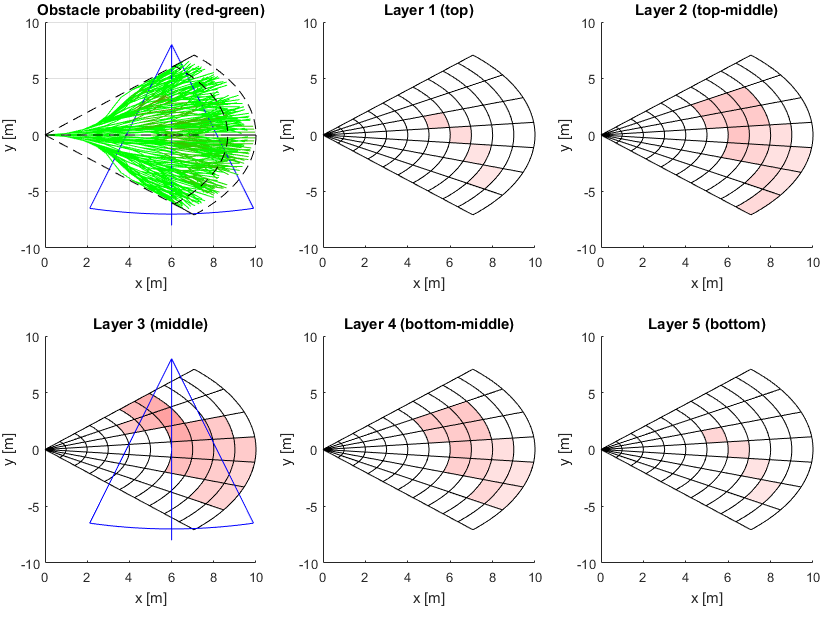
\includegraphics[width=\textwidth]{\FIGDIR/P18SpreadTimedObstacleSpace}
    \caption{Obstacle space for static uncertainty spread}
    \label{fig:P18SpreadTimedObstacleSpace}
\end{figure}
\noindent  Similar to fig. \ref{fig:P16SpreadStaticObstacleSpace} only time aspect is now accounted.

\begin{figure}[H]
    \centering
    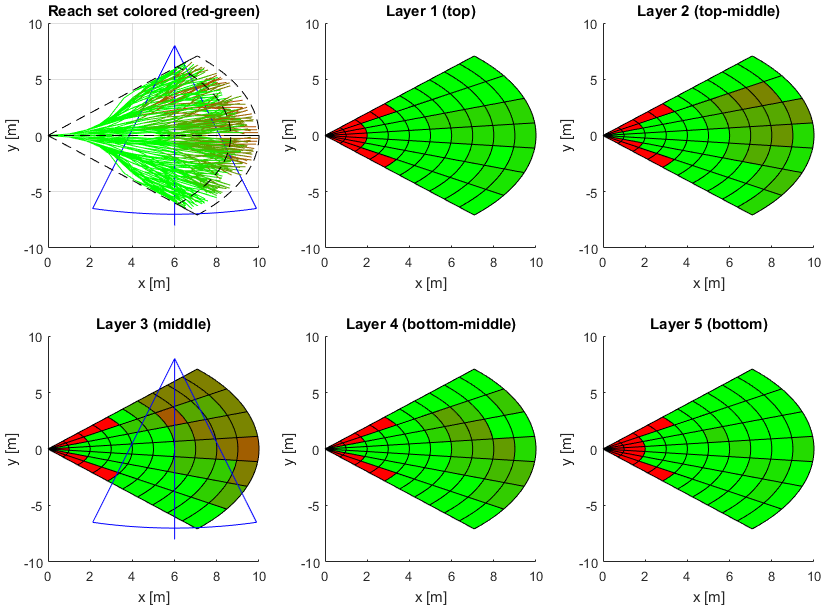
\includegraphics[width=\textwidth]{\FIGDIR/P19SpreadTimedReachSet}
    \caption{Reach set approximation for static uncertainty spread - all layers}
    \label{fig:P19SpreadTimedReachSet}
\end{figure}
\noindent  Similar to fig. \ref{fig:P17SpreadStaticReachSet} only time aspect is now accounted.

\section{Static obstacles avoidance}\label{sec:staticObstacleAvoidanceSimulation}
\noindent \emph{Static obstacle avoidance} testing scenario has been introduced in \cite{alojzgomola2017}. This chapter will introduce only a brief introduction to the test. The vehicle equipped with LiDAR sensor and ADS-B transceiver/receiver is flying in uncharted territory and executing a mission consisting from waypoint set $\mathscr{WP}$. The simulation is executed in mission local coordinate frame, where the vehicle initial position is center of frame and vehicle heading is aligned with main axis.

\noindent The ordered waypoint set $\mathscr{WP}$ is defined as follow:
\begin{enumerate}
    
    \item\emph{Starting waypoint $W_1$} - $[0,0,0]$ - not necessary, just to emphasize the local coordinate frame center
    \item\emph{First obstacle waypoint $W_2$} - $[20,0,0]$.
    \item\emph{Second obstacle waypoint $W_3$} - $[20,20,0]$.
    \item\emph{Third obstacle waypoint $W_4$} - $[0,20,0]$.
    \item\emph{Final waypoint $W_5$} - $[0,0,10]$.
\end{enumerate}

\noindent The obstacle set $\mathscr{O}$ is defined as set of ball obstacles $\mathscr{O}_{\mathscr{B}}(\vec{p},r)$, where $\vec{p}$ indicates obstacle center position and $r$ stands for obstacle radius. The testing obstacle set was defined as follow set of map/detected obstacles $\mathscr{O}_M=\mathscr{O}_D$:
\begin{enumerate}
    \item\emph{First obstacle $\mathscr{B}_\mathscr{O}(1)$} -  $\mathscr{O}_{\mathscr{B}}(\vec{p}=[10,0,0],r=2)$
    \item\emph{Second obstacle $\mathscr{B}_\mathscr{O}(2)$} - $\mathscr{O}_{\mathscr{B}}(\vec{p}=[20,10,0],r=2)$
    \item\emph{Third obstacle $\mathscr{B}_\mathscr{O}(3)$} - 
    $\mathscr{O}_{\mathscr{B}}(\vec{p}=[10,20,0],r=2)$
\end{enumerate}

\noindent Other simulation parameters are stated like follows:
\begin{enumerate}
    \item\emph{Vehicle model $\dot{x}=f(x,u)$} is given by eq. \ref{eq:simple3ddifferentialequations}.
    \item\emph{Vehicle control $\mathscr{MA}$} is defined in section \ref{ch:movementAutomatonPredictor}.
    \item\emph{Vehicle body radius $r_b$} is given as 30 cm.
    \item\emph{Vehicle turning radius $r_t$} is given as 2 m, this parameter impacts the decision time $t_i$ selection based on the in-veritable crash distance \cite{alojzgomola2017}.
    \item\emph{Movement automaton prediction error $E_p=(\mathscr{MA}$)} is equal to 30 cm.
    \item\emph{Safety margin $s_m$} is set to 60 cm.
    \item\emph{Avoidance grid $A(t_i) $}properties were set as follow:
    \begin{enumerate}[a.]
        \item start distance $d_s$ 0 m,
        \item end distance $d_e$ 10 m,
        \item step distance $s_d$ 1 m (10 layers),
        \item horizontal span from $\theta_s$ as $-\pi/4$ to $\theta_e$ to $\pi/4$,
        \item horizontal cell count $c_h$ as $7$,
        \item vertical span from $\varphi_s$ as $-\pi/6$ to $\varphi_e$ to $\pi/6$,
        \item vertical cell count $c_v$ as $5$ (layer count).
    \end{enumerate}
\end{enumerate}

\noindent \emph{Note:} The obstacles are proposed as convex obstacles, the real world obstacles usually breaches the convex surface assumption, the approach was tested on non convex obstacles and open traps. The simplicity of testing example is given to show main properties of approach. Comparison to deterministic approach performance can be made by comparing section 6 of \cite{alojzgomola2017}.

\noindent Legend of simulation results is following:
\begin{enumerate}
    \item\emph{Executed trajectory} (blue line) - executed trajectory by vehicle at moment of snapshot
    \item\emph{Planned trajectory} (red line) - planned trajectory within avoidance grid $\mathscr{A}(t_i)$, trajectory is re-planned every decision time $t_i$. Note that in case of this simulation the trajectory was re-planned every movement.
    \item\emph{Waypoints} (green square markers) - mission plan for multiple waypoints. 
    \item\emph{Obstacles} (red point clouds) - obstacle sets break into point clouds.
    \item\emph{Field of vision} (black dashed line) - denotes current avoidance grid $\mathscr{A}(t_i)$ boundary starting at vehicle position at time of snapshot.
\end{enumerate}
    
\noindent Following decisive moment have been taken into consideration when making snapshots:
\begin{enumerate}
    \item\emph{First obstacle set $\mathscr{B}_\mathscr{O}(1)$ avoidance} (fig. \ref{fig:P31FirstObstacleAvoidance}) - vehicle is heading straight to the obstacle center, the moment captured is when vehicle is avoiding the obstacle. The obstacle is fully covered by field of the vision and vehicle is avoiding it from right side without breaching the safety margin $s_m$. 
    \item\emph{Second obstacle set $\mathscr{B}_\mathscr{O}(2)$ avoidance} (fig. \ref{fig:P35SecondObstacleAvoidance}) - The vehicle is avoiding the second obstacle after the turn, the obstacle is partially in vehicles FOV. The vehicle will crash if there was not a movement restriction given by restriction of reachability property $P_{R}(c_{i,j,k}), \forall c_{i,j,k}\in\mathscr{A}(t_i)$
    \item\emph{Third obstacle set $\mathscr{B}_\mathscr{O}(3)$ avoidance} (fig. \ref{fig:P36ThirdObstacleAvoidance}). - Same as second obstacle. Please note that the cost function $J^*(\mathscr{T}(\vec{x}_0,B))$ is designed to prioritize planar movements. The horizontal/vertical separation was not used in this framework and cost can impact the decision making. 
    \item\emph{Vehicle trajectory after mission competition} (fig. \ref{fig:P37FullAvodanceStaticObstacle}) - The overview of trajectory and decisions, it is assumed that all paths between $W_4$ and $W_5$ are not obscured, this is to show, that avoidance grid $\mathscr{A}(t_i)$ can generate smooth trajectories in free space.
\end{enumerate}

\begin{figure}[H]
    \centering
    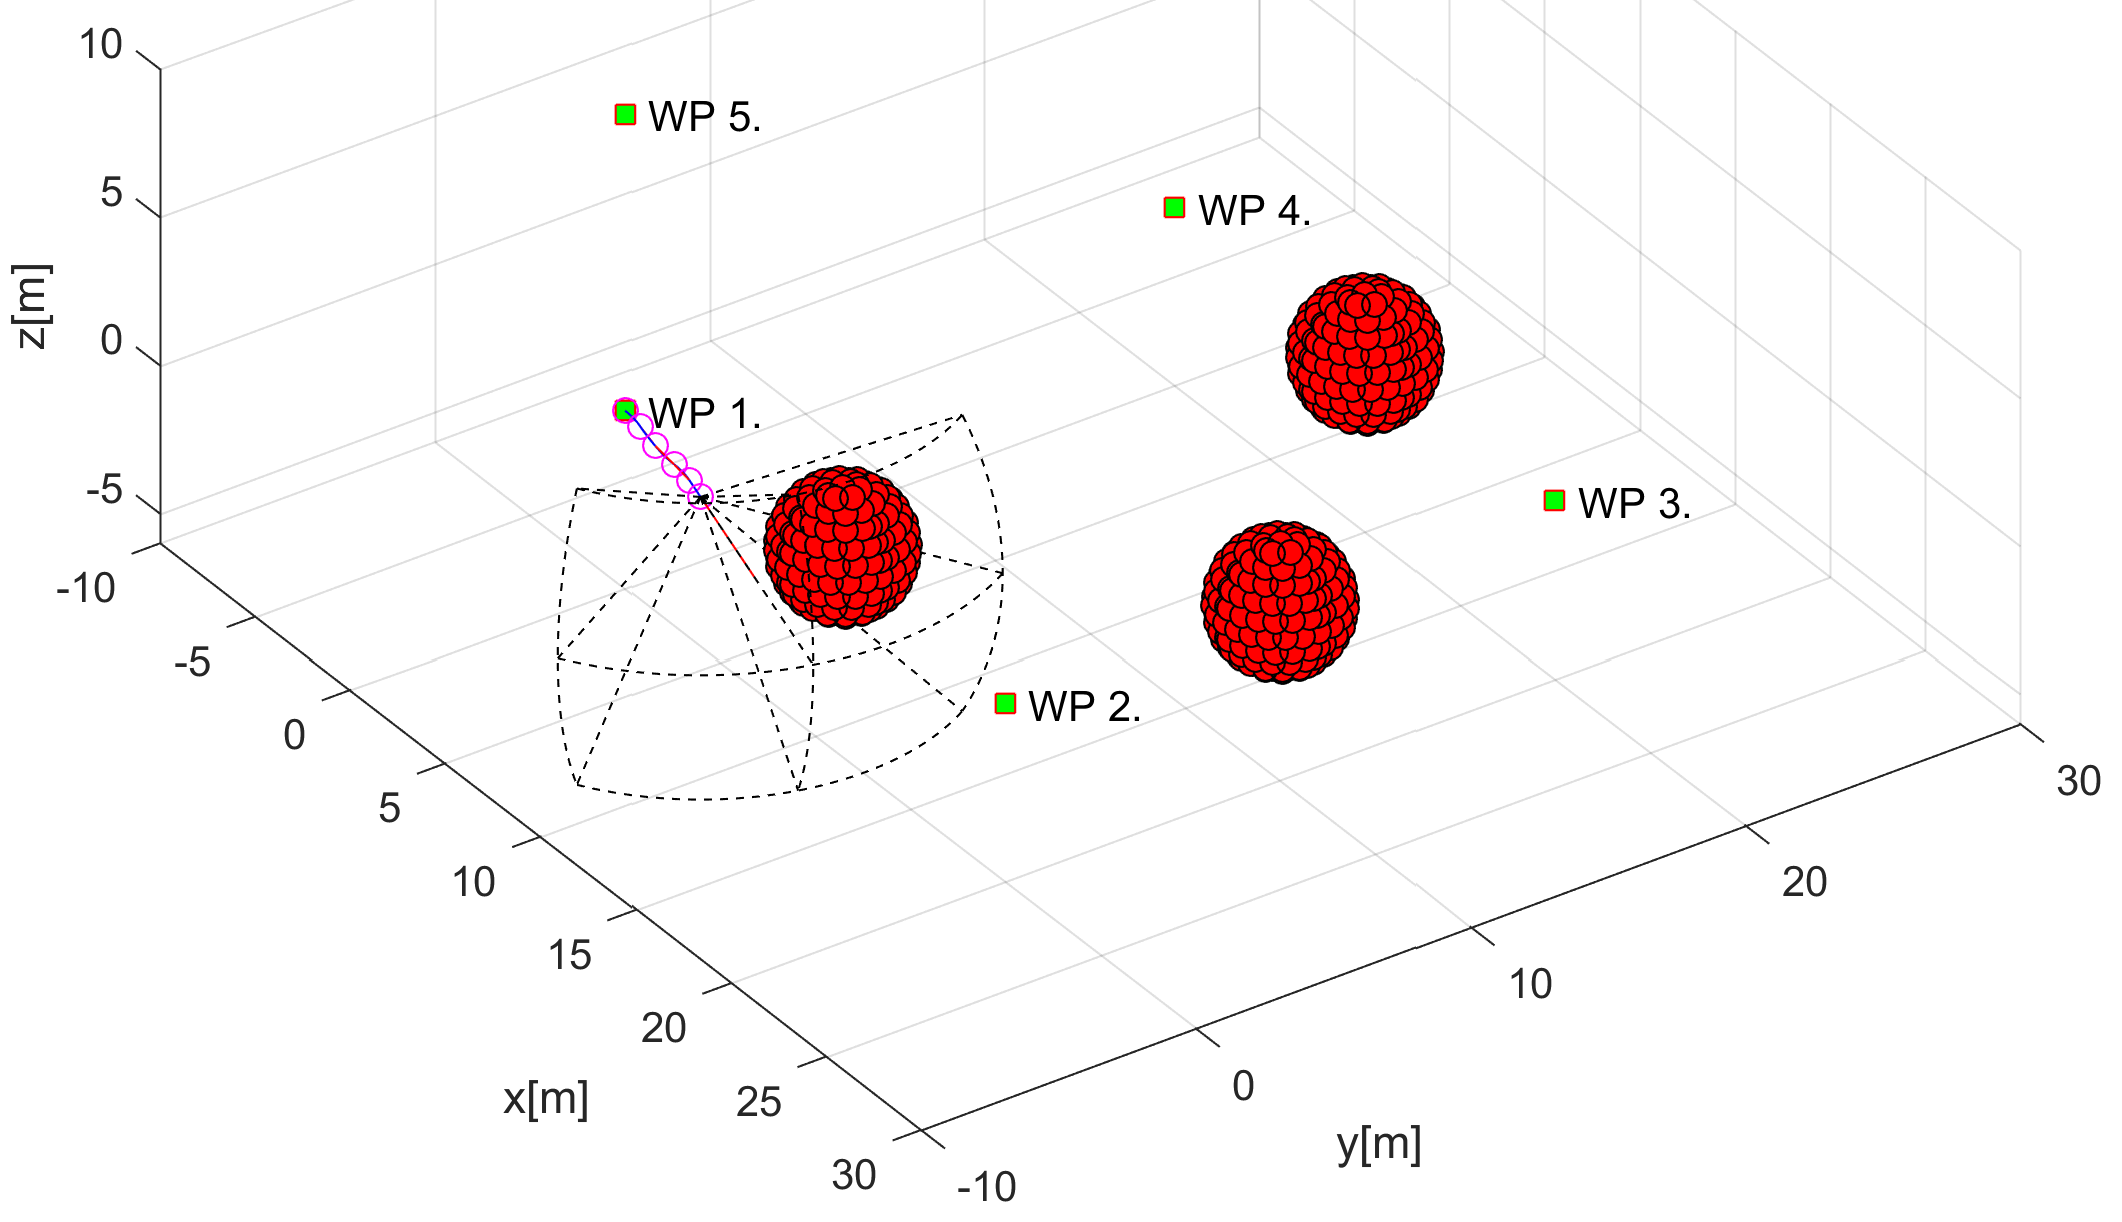
\includegraphics[width=\textwidth]{\FIGDIR/P31FirstObstacleAvoidance}
    \caption{First obstacle set $\mathscr{B}_\mathscr{O}(1)$ avoidance}
    \label{fig:P31FirstObstacleAvoidance}
\end{figure}

\begin{figure}[H]
    \centering
    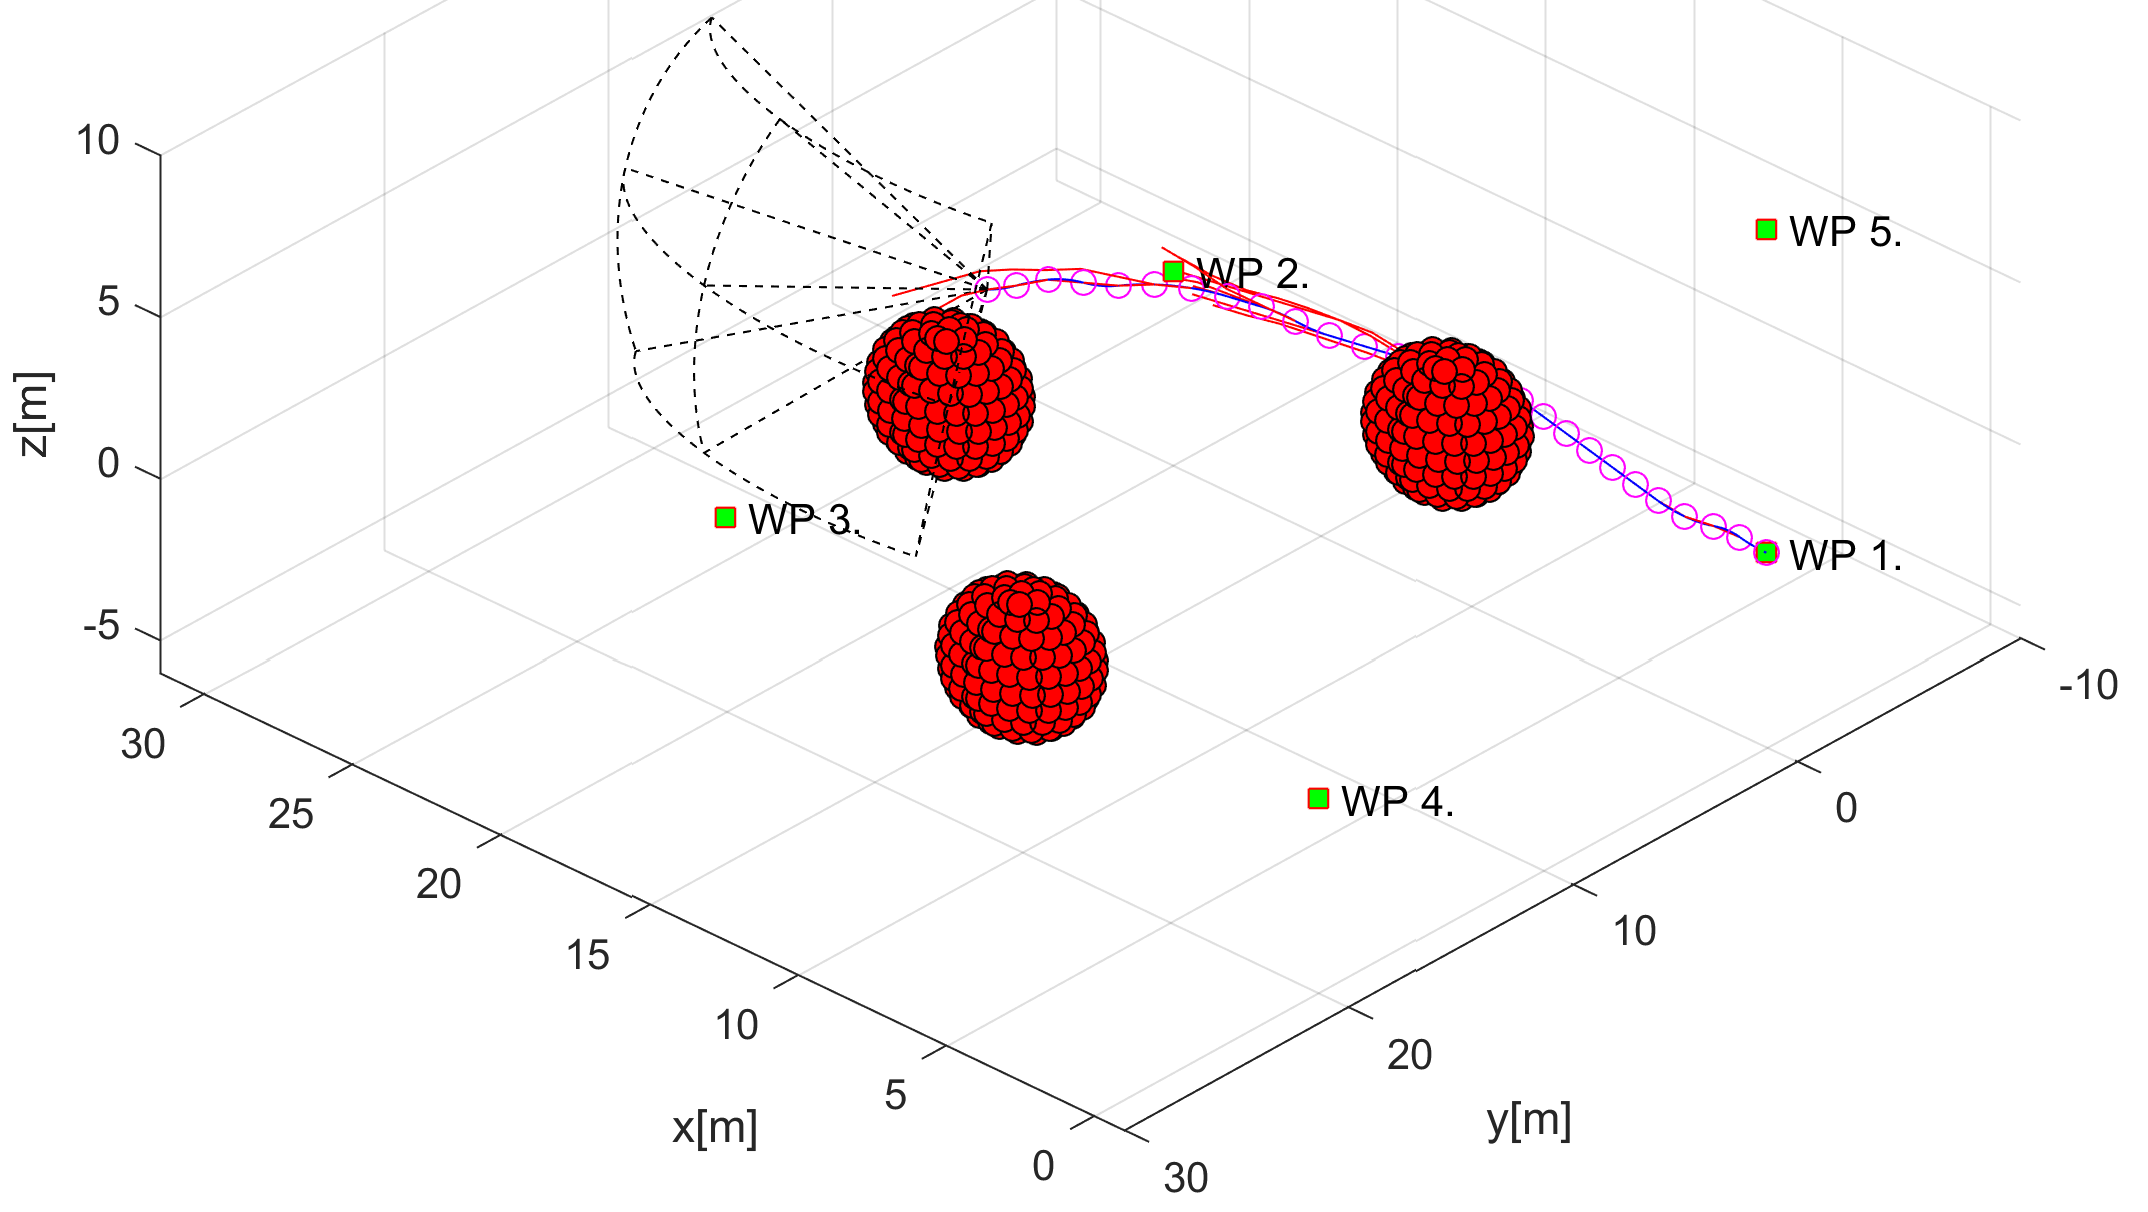
\includegraphics[width=\textwidth]{\FIGDIR/P35SecondObstacleAvoidance}
    \caption{Second obstacle set $\mathscr{B}_\mathscr{O}(2)$ avoidance}
    \label{fig:P35SecondObstacleAvoidance}
\end{figure}

\begin{figure}[H]
    \centering
    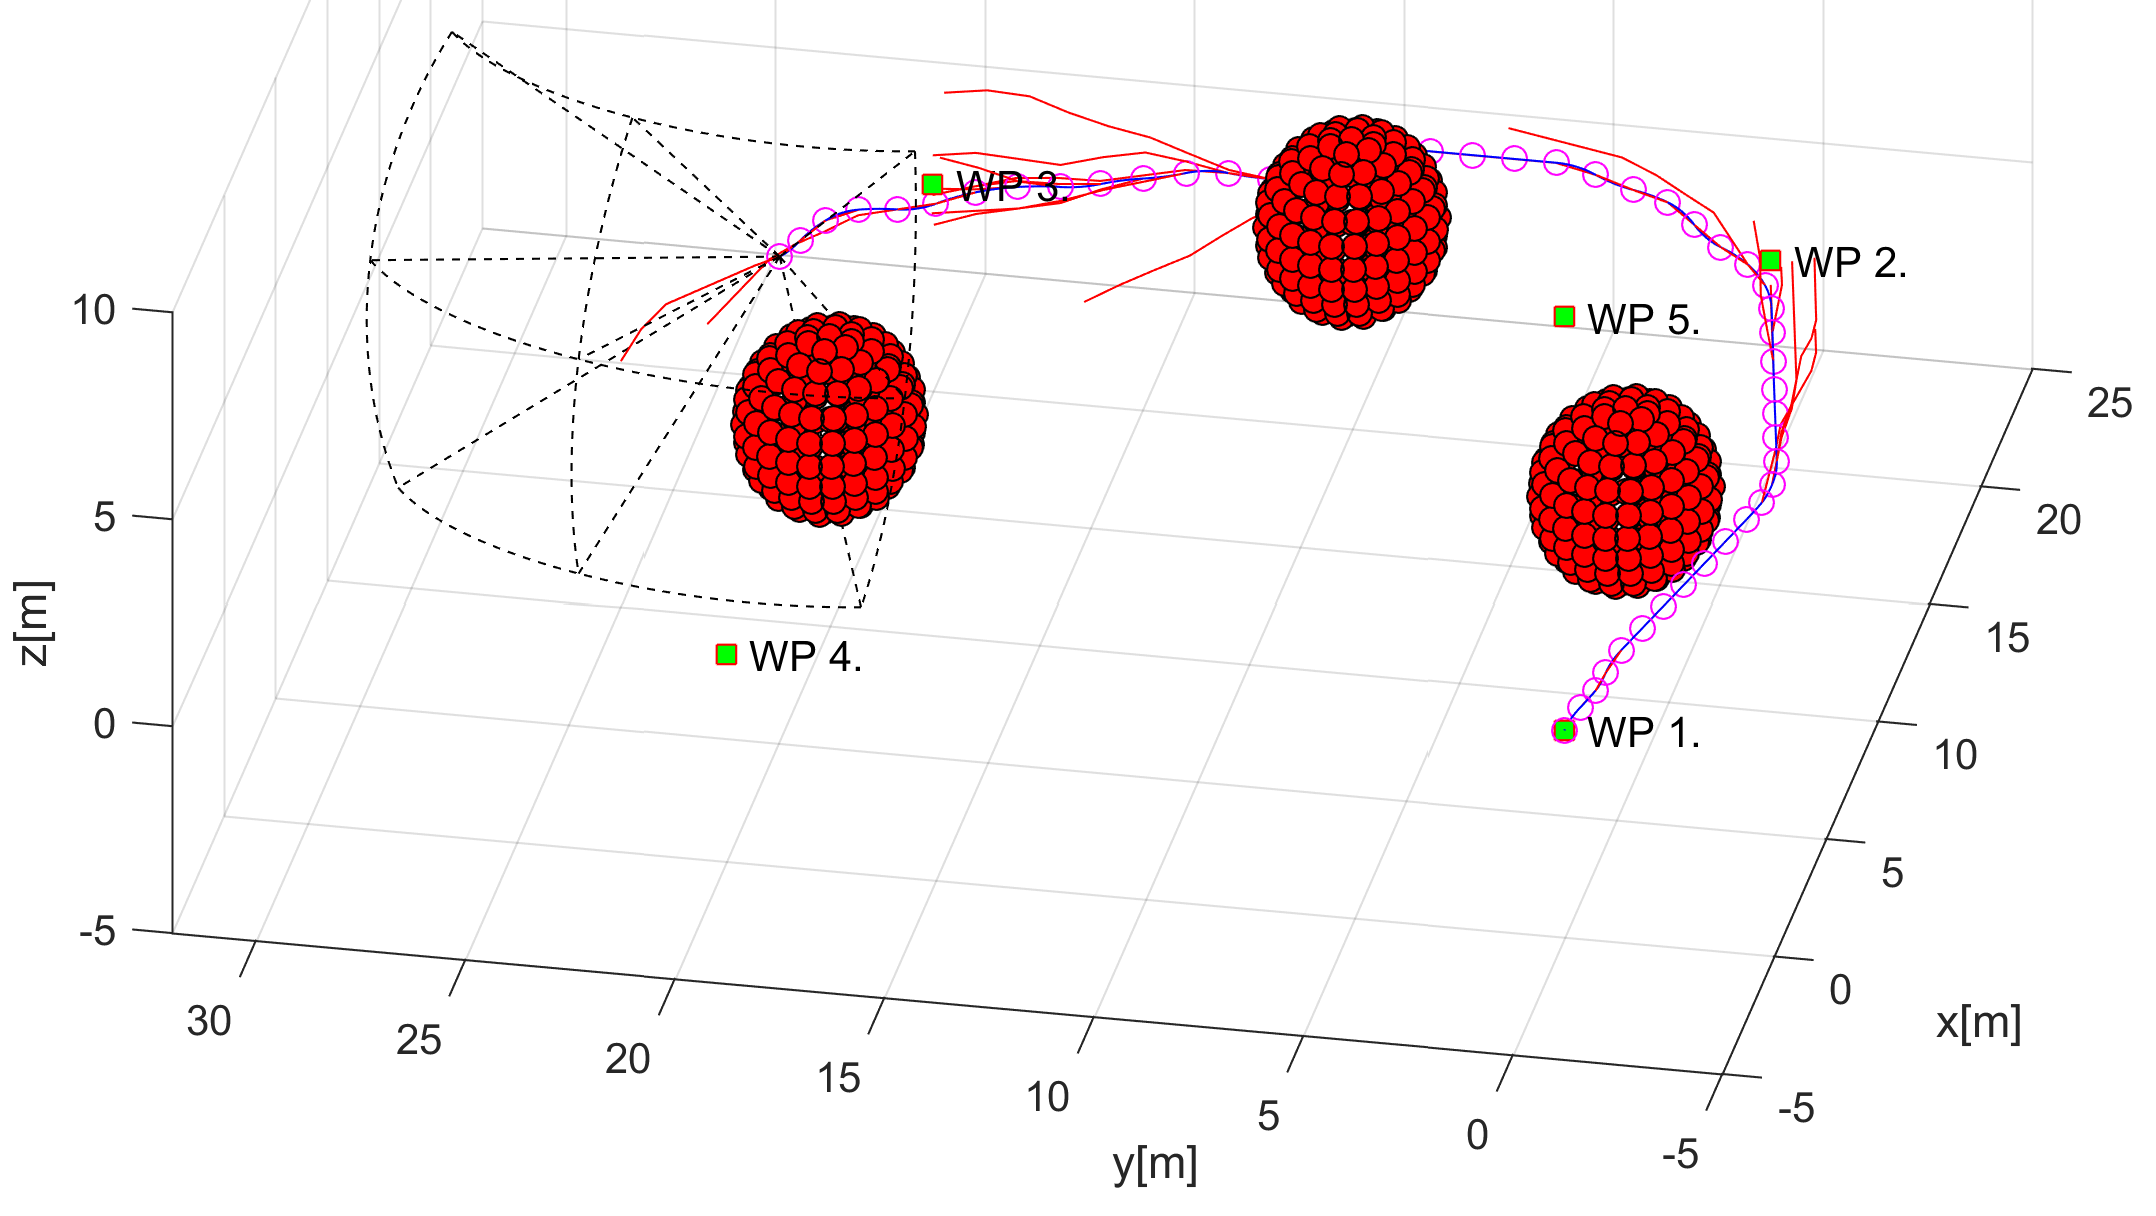
\includegraphics[width=\textwidth]{\FIGDIR/P36ThirdObstacleAvoidance}
    \caption{Third obstacle set $\mathscr{B}_\mathscr{O}(3)$ avoidance}
    \label{fig:P36ThirdObstacleAvoidance}
\end{figure}

\begin{figure}[H]
    \centering
    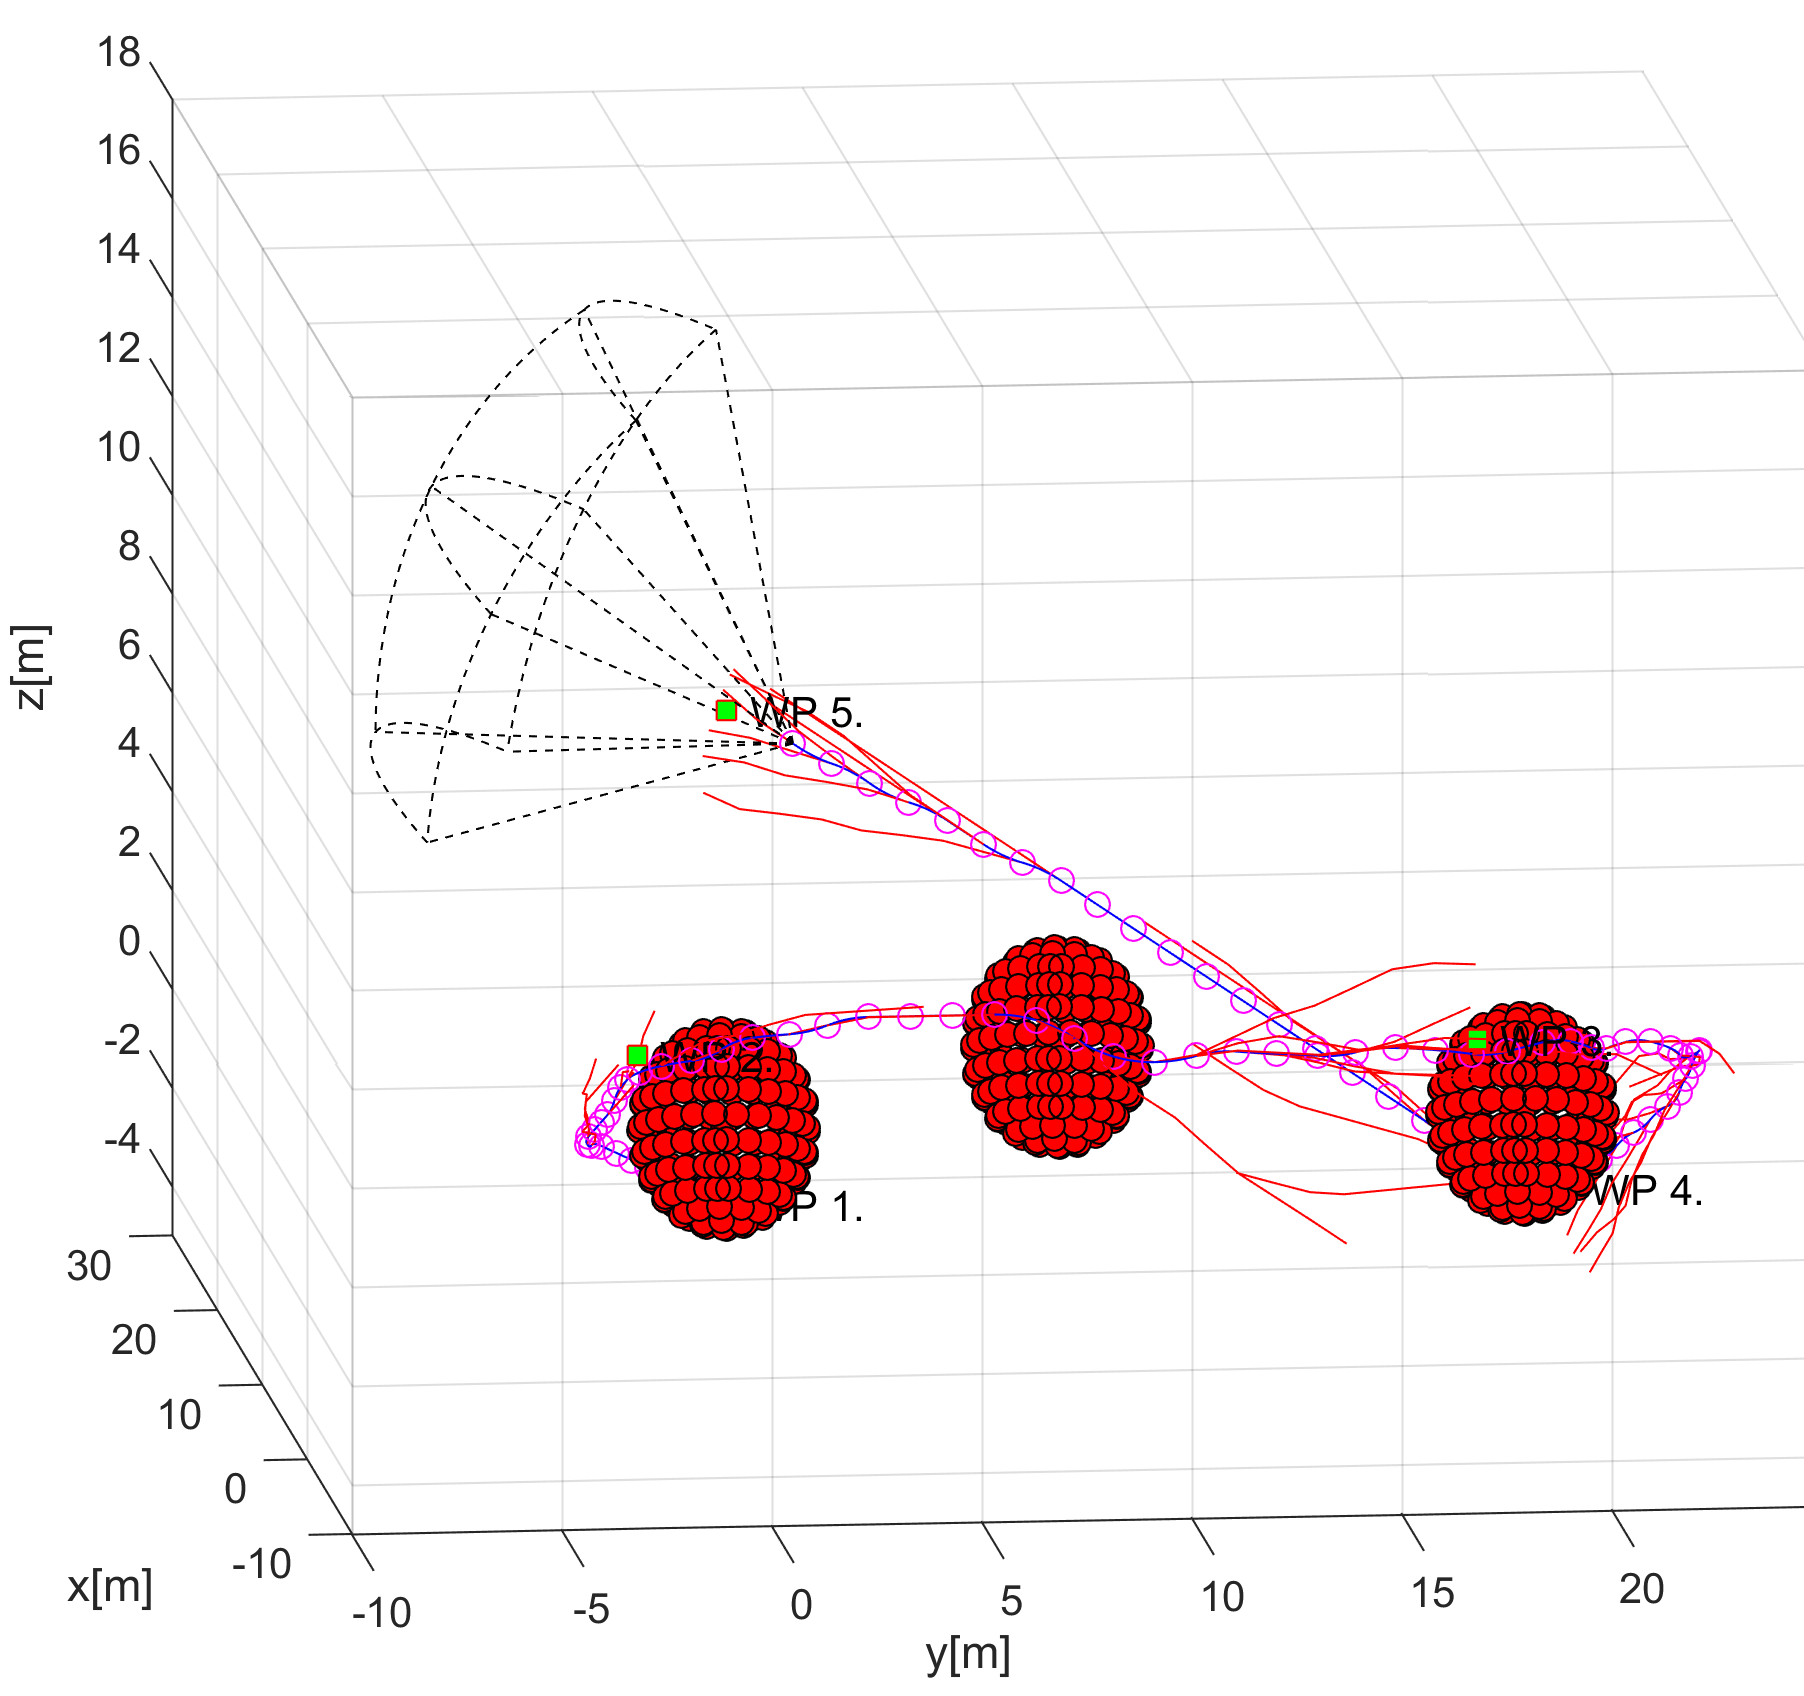
\includegraphics[width=\textwidth]{\FIGDIR/P37FullAvodanceStaticObstacle}
    \caption{Vehicle trajectory after mission competition}
    \label{fig:P37FullAvodanceStaticObstacle}
\end{figure}

\subsection{Probabilistic model evaluation}\label{sec:probabilisticModelEvaluation}
\noindent The \emph{general algorithm} (\ref{eq:mainRatingInputs},\ref{eq:mainRatingCalculation}), defines multiple probabilities for cells $c_{i,j,k}\in\mathscr{A}$ and trajectories $\mathscr{T}\in\mathscr{R}$, in case of static obstacle avoidance the key focus probabilities are following:
\begin{enumerate}
    \item\emph{Reachibility probability} $P_{R}(c_{i,j,k})$, $P_{R}(\mathscr{T}(x_0,B))$ - the the reachability was impacted by obstacle space $\mathscr{O}$ and visibility, for sake of simplicity the reachability was reaching only two values $P_{R}\in \{0,1\}$ .
    \item\emph{Obstacle probability} $P_{O}(c_{i,j,k})$ - obstacle probability in cell was assessed using general algorithm (\ref{eq:mainRatingInputs},\ref{eq:mainRatingCalculation}) and detected obstacle probability $P_{O_D}$ (\ref{eq:detectedObstacleProbability}).
    \item\emph{Visibility probability} $P_{O}(c_{i,j,k})$ - calculated according to standard visibility formula $P_V(c_{i,j,k})$ (\ref{eq:FinalVisibilityProbability}).
\end{enumerate}


\begin{figure}[H]
    \centering
    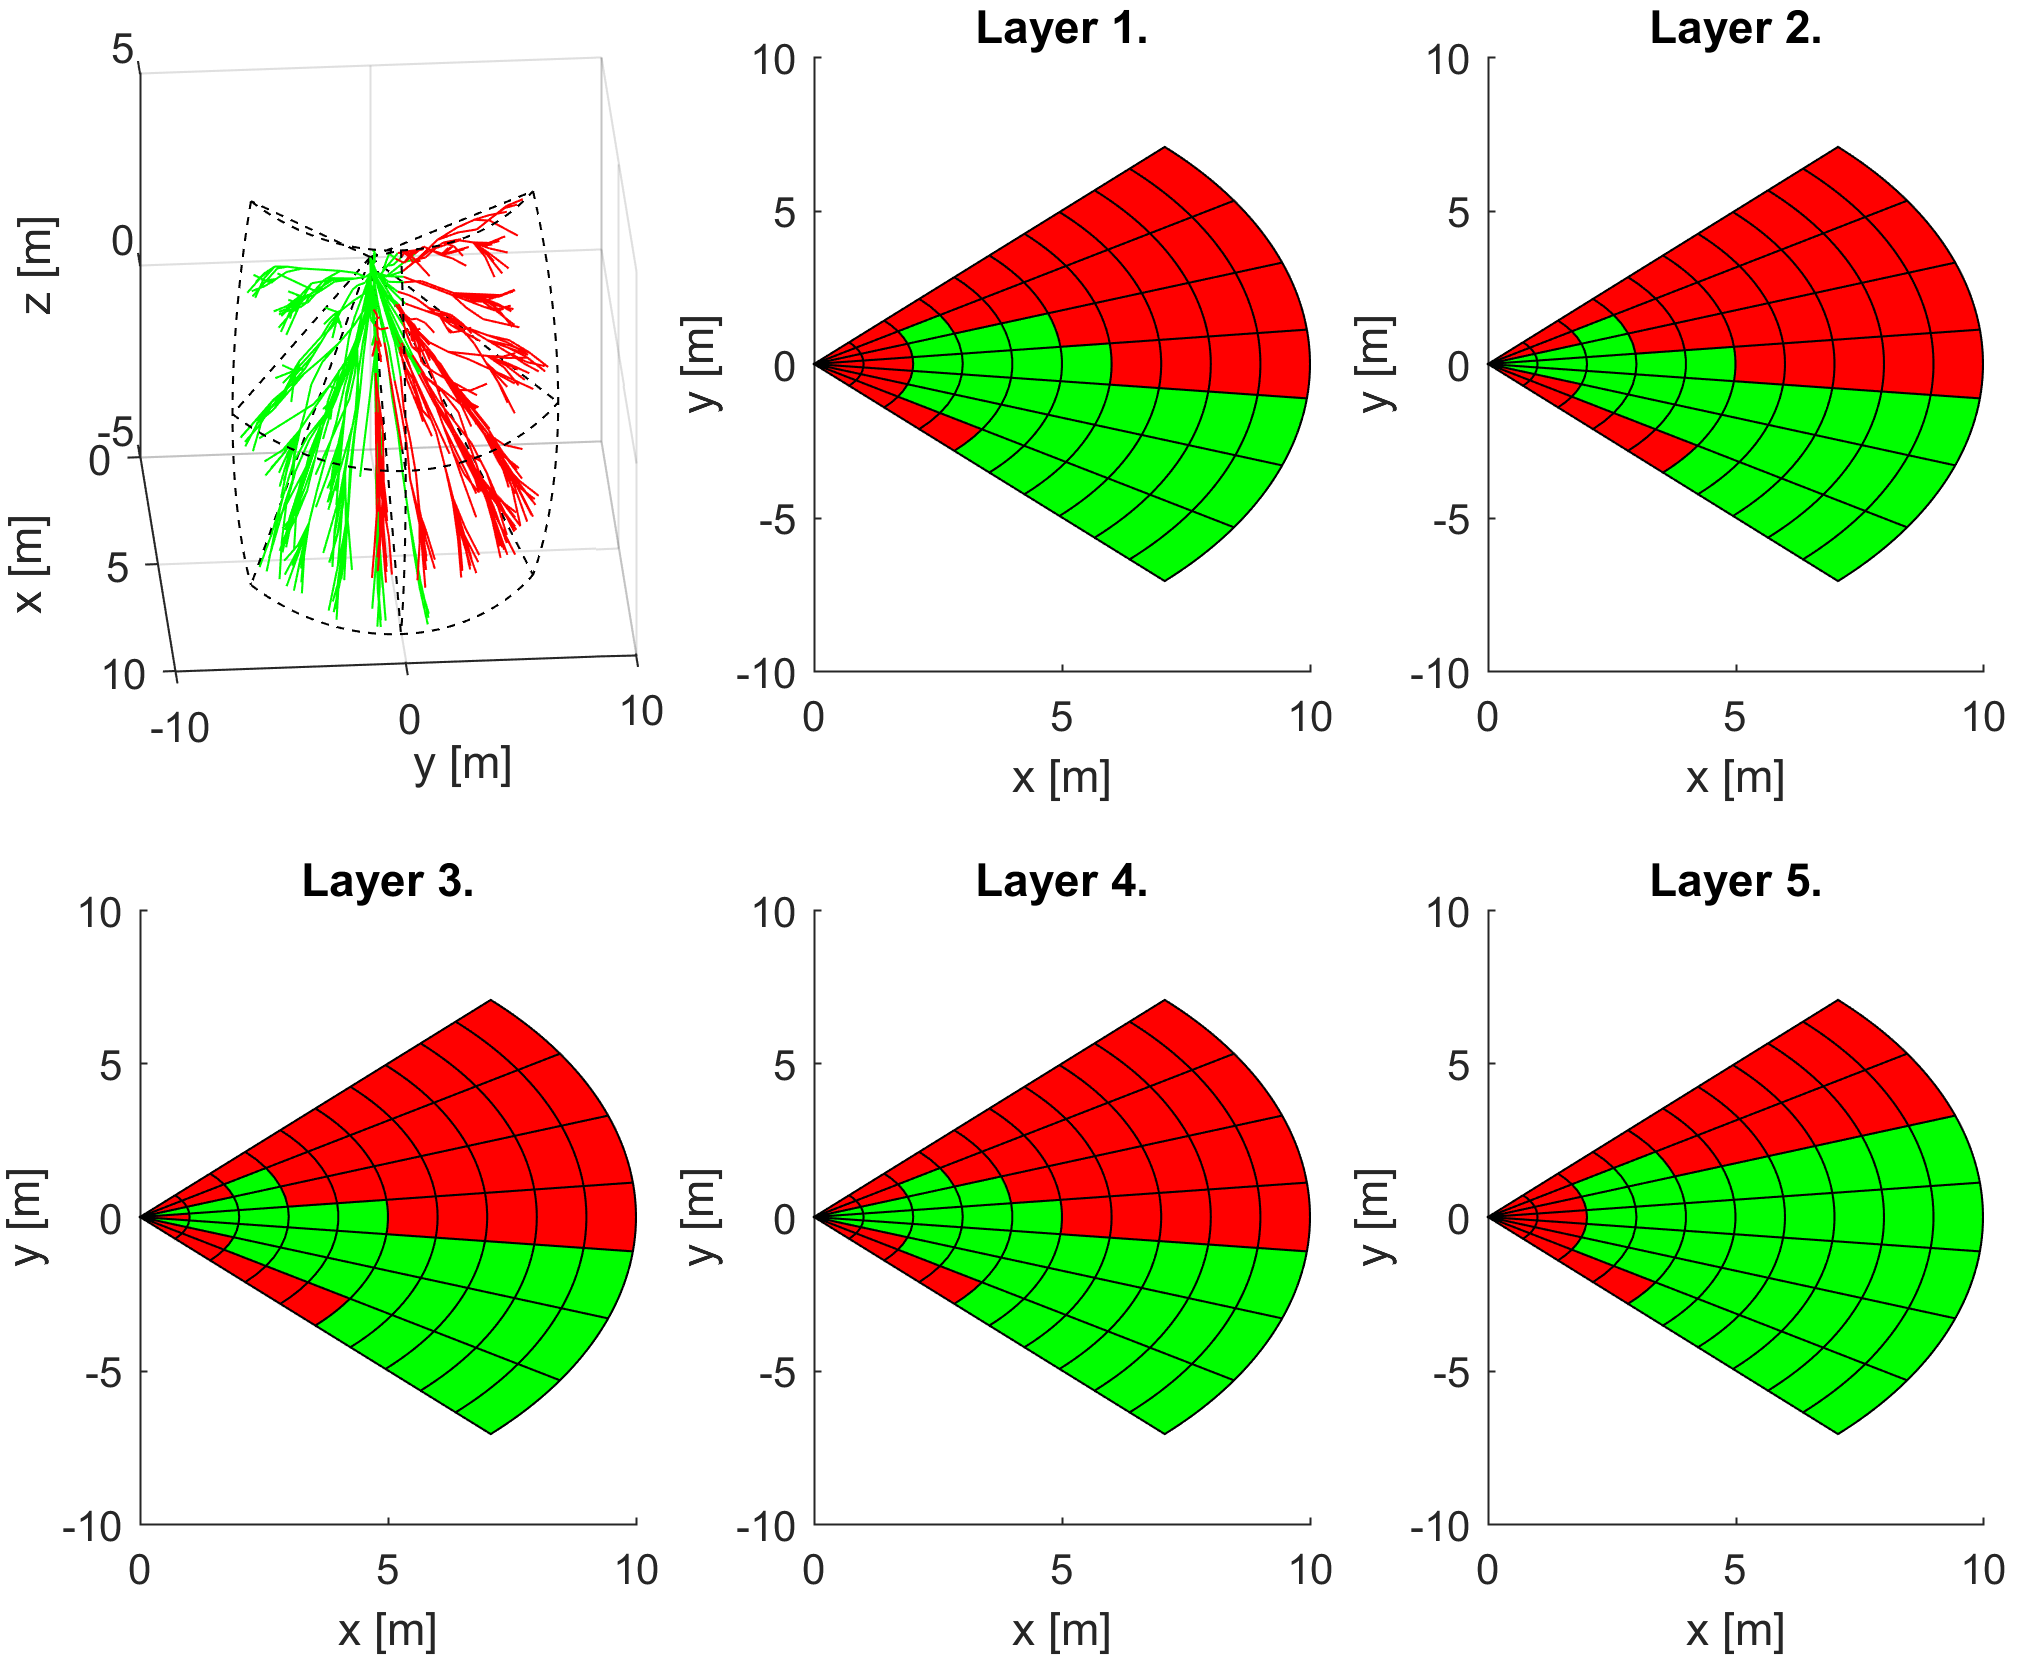
\includegraphics[width=\textwidth]{\FIGDIR/P32ReachableSpaceExampleStatic}
    \caption{Reachability probability assessment for $\mathscr{B}_\mathscr{O}(1)$ avoidance}
    \label{fig:P32ReachableSpaceExampleStatic}
\end{figure}
\noindent For intersection please refer to \emph{first obstacle set $\mathscr{B}_\mathscr{O}(1)$ avoidance} (fig. \ref{fig:P31FirstObstacleAvoidance}). The obstacle space is slightly in right-upper quadrant (from vehicles viewpoint). The red trajectories are leading to obstacle or trough obstacle space, the green trajectories are leading trough or to safe space. \emph{Layer 1.-5.} right part is not reachable (red cells), there is possible escape paths on left side (green cells).

\begin{figure}[H]
    \centering
    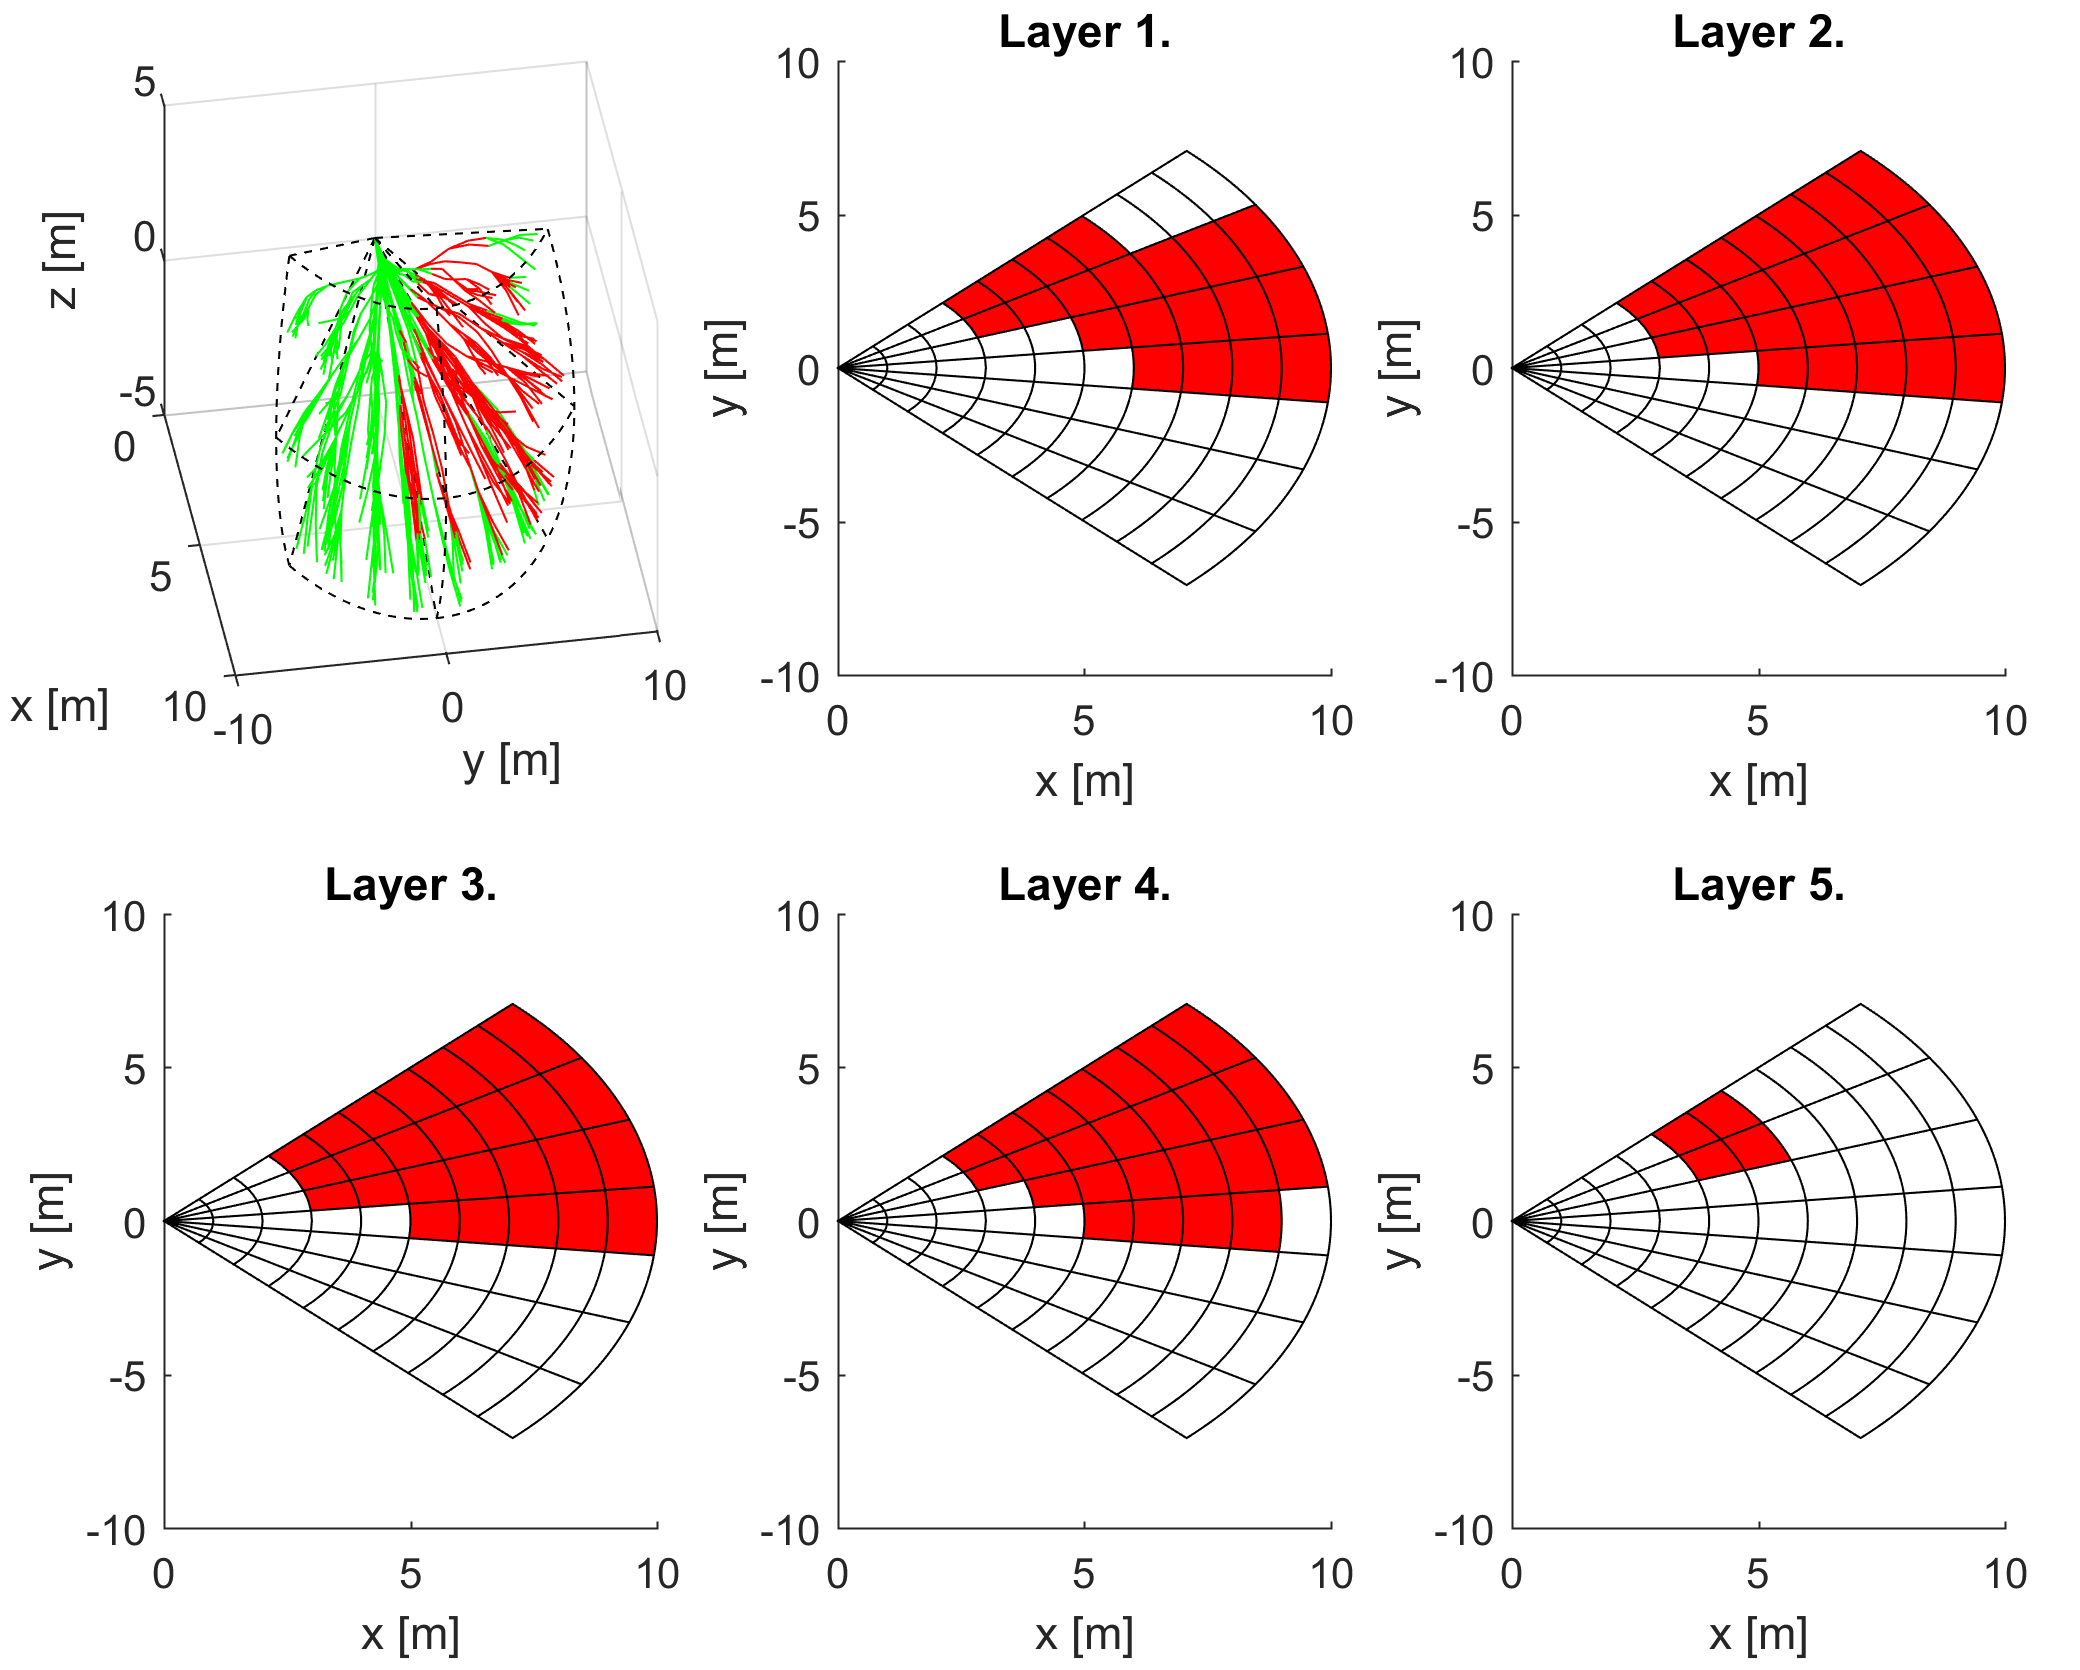
\includegraphics[width=\textwidth]{\FIGDIR/P33ObstacleSpaceStaticExample}
    \caption{Obstacle probability assessment for $\mathscr{B}_\mathscr{O}(1)$ avoidance}
    \label{fig:P33ObstacleSpaceStaticExample}
\end{figure}
\noindent For intersection please refer to \emph{first obstacle set $\mathscr{B}_\mathscr{O}(1)$ avoidance} (fig. \ref{fig:P31FirstObstacleAvoidance})
The obstacle space is slightly in right-upper quadrant (from vehicles viewpoint). The red trajectories are leading to obstacle or trough obstacle space, the green trajectories are leading trough or to safe space. The obstacle space accounts only visible part of the obstacle, therefore in \emph{layer 1. and 4.} is space which is considered without obstacle (white cells). The obstacle space (red cells) in bottom layer (\emph{layer 5.}) is very small due the vehicle is tilted down a little in time of obstacle assessment.

\begin{figure}[H]
    \centering
    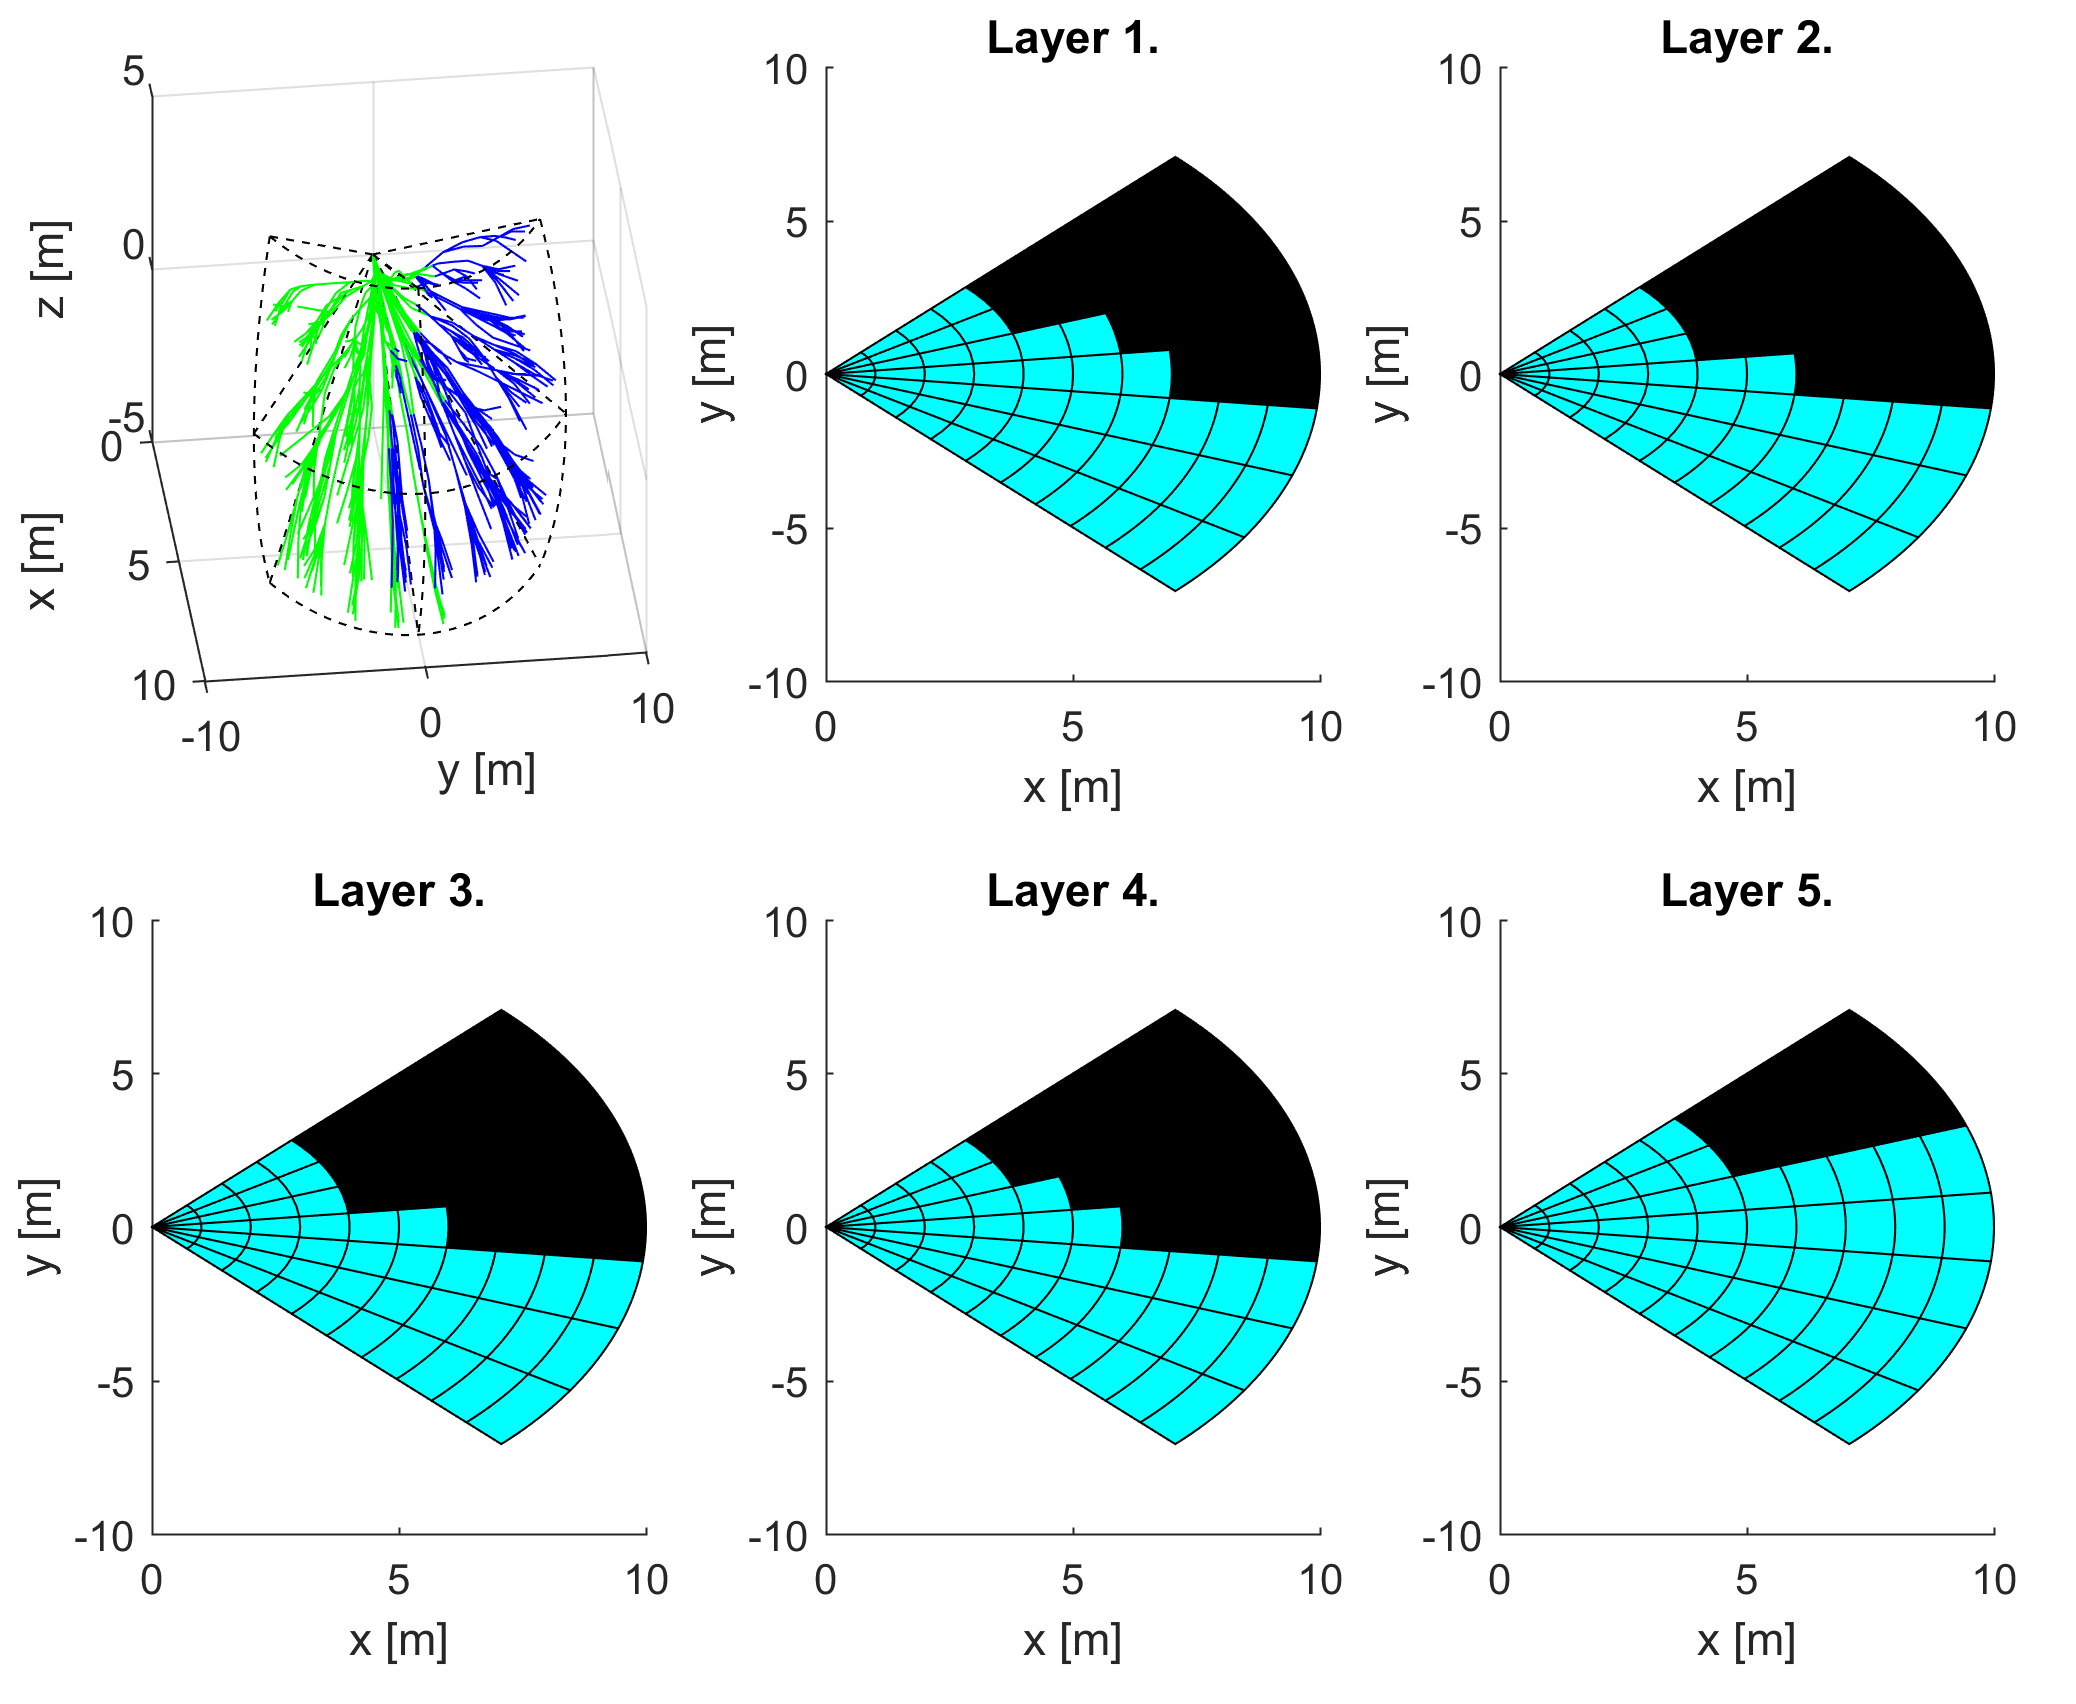
\includegraphics[width=\textwidth]{\FIGDIR/P34VisibleSpaceStaticExample}
    \caption{Visibility probability assessment for $\mathscr{B}_\mathscr{O}(1)$ avoidance}
    \label{fig:P34VisibleSpaceStaticExample}
\end{figure}
\noindent For intersection please refer to \emph{first obstacle set $\mathscr{B}_\mathscr{O}(1)$ avoidance} (fig. \ref{fig:P31FirstObstacleAvoidance}). 
The \emph{visibility space is obscured }


\subsection{Avoidance performance}\label{sec:avoidancePerformacne}
\noindent \emph{Obstacle avoidance performance} for autonomous systems is evaluated by multiple criteria. A necessary condition is \emph{crash distance $d_c$ does not cross safety margin $s_m$}. In the other world that vehicle does not crash into static obstacle. 

\emph{The sufficient conditions} are following:
\begin{enumerate}
    \item\emph{Energy consumption} - For each system $\dot{x}=f(x,u)$ cost functional $J(x,u,t)$ can be proposed to reflect system performance or energy consumption. This functional is therefore used in optimization maximization/minimization problem.
    \item\emph{Trajectory tracking} - Trajectory of vehicle is given by ordered set of waypoints $\mathscr{WP}=\{W_1,W_2,\dots,W_i\}$. The given trajectory may not be feasible for vehicle system $\dot{x}=f(x,u)$. To differentiate the performance of tracking Mean Square error is introduced like following:
    \begin{equation}
        e= \sqrt{\left((\hat{x}(t)\to\R^k)-(x(t)\to\R^k)\right)^2}
    \end{equation}
    \noindent Where $(\hat{x}(t)\to\R^k)$ is expected parameters projected to space $\R^k$ and $(x(t)\to\R^k)$ is real system performance projected to same space. Usually performance parameter is deffined as deviation from projected trajectory $\tilde{x}(t)\in\R^3$.
\end{enumerate}

\begin{figure}[H]
    \centering
    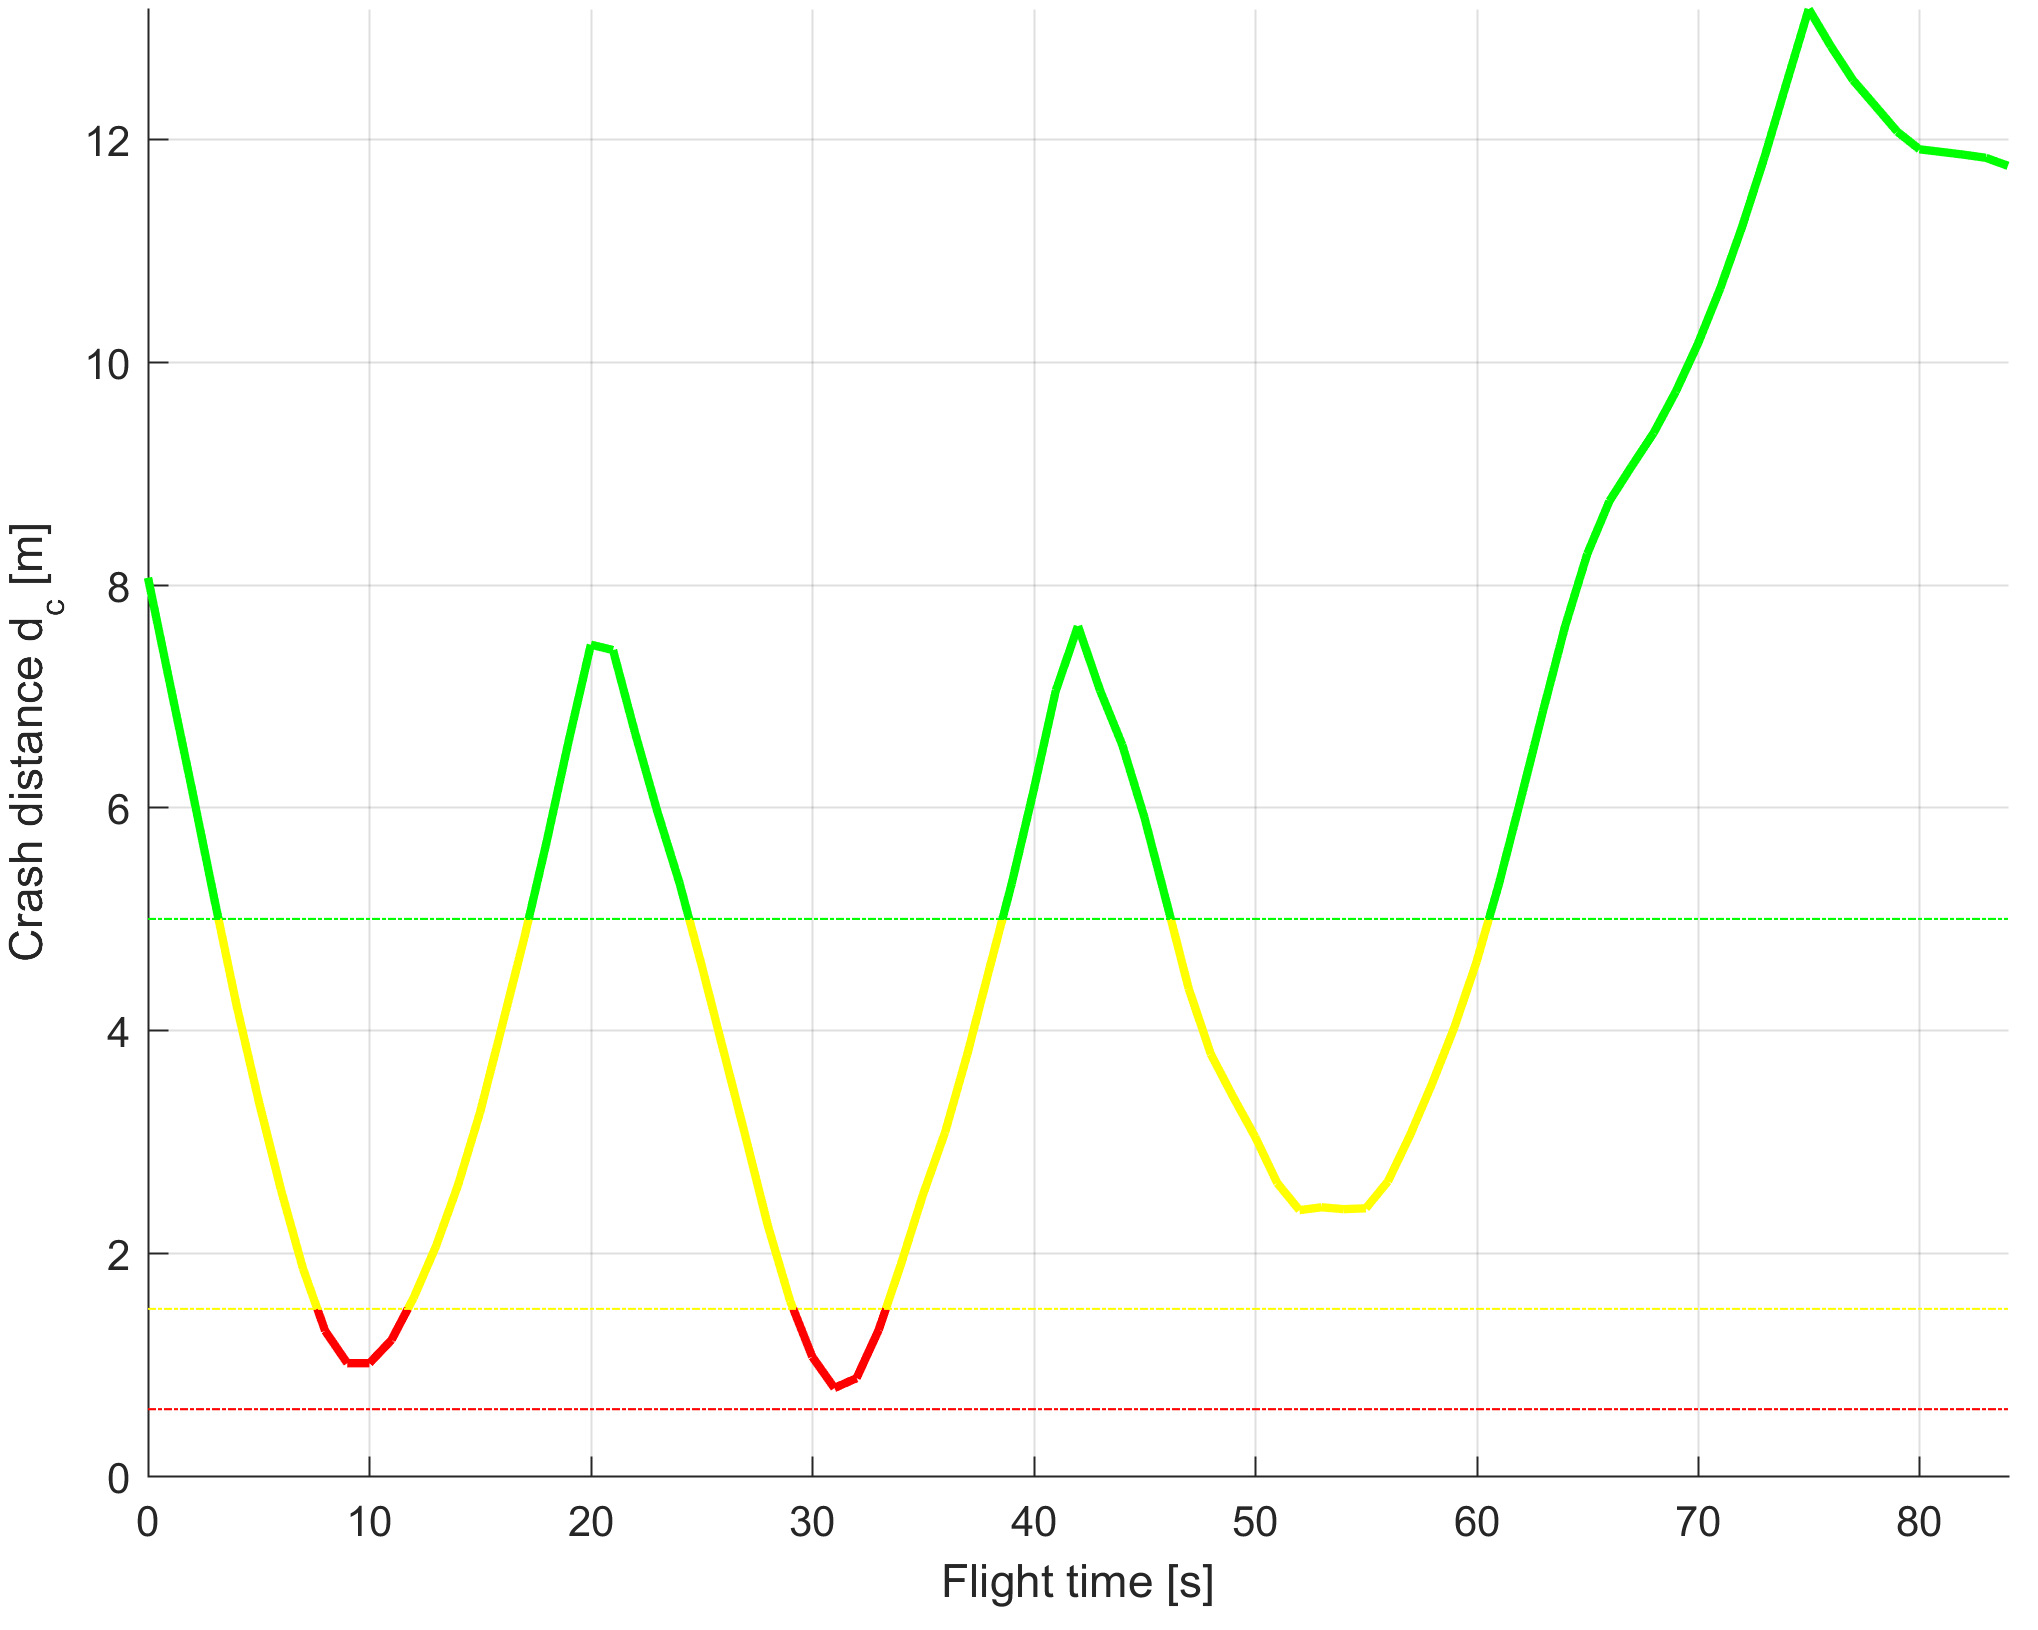
\includegraphics[width=\textwidth]{\FIGDIR/P38CrashDistanceEvolutionWide}
    \caption{Crash distance $c_r$ evolution during mission}
    \label{fig:P38CrashDistanceEvolutionWide}
\end{figure}

\noindent \emph{Crash distance to nearest obstacle evolution} (fig \ref{fig:P38CrashDistanceEvolutionWide}) displays how far vehicle was to nearest obstacle during the mission execution. There are three lines representing:
\begin{enumerate}
    \item\emph{Conservative methods margin $c_m$} (green dashed line) - conservative methods are based on simple preposition \emph{turn back while you can}, therefore conservatives methods margin $c_m$ is calculated like follow:
    \begin{equation}
        c_m = 
        \begin{aligned}
            &2\times r_t + 3 \times r_v\\
            &2 \times 2m + 3\times 0.6m\\
            &4.6m
        \end{aligned}
    \end{equation}
    \noindent Where $r_t$ is turning radius of vehicle and $r_v$ is radius of vehicle. The conservative methods margin $c_m$ is $4.6$ meters for given simulation parameter. 
    
    \item\emph{Adaptive methods margin $a_m$} (yellow dashed line) - are more energy consumption focused. The focus is on not deviating from optimal trajectory as long as possible. Typical representative of adaptive algorithms is potential field avoidance algorithm. The \emph{potential field avoidance} principle is following: Each  obstacle (static or moving) has a potential like a magnet, our vehicle has inverse potential. The magnitude of potentials can change over time depending on various factors (like the danger level etc.). The margin of adaptive methods was calculated by following formula:
    \begin{equation}
        a_m = 6 \times r_v = 6 times 0.3 = 1.8 m
    \end{equation}
    \noindent Where $r_v$ stands for vehicle radius. The adaptive methods margin $a_m$, where the \emph{potential field method} is key comparison element is $1.8$ m
    
    \item\emph{Safety margin $s_m$} (red dashed line) has been discussed in section \ref{sec:staticObstacleAvoidanceSimulation}. Safety margin of our method $s_m$ is set as $60 cm$
\end{enumerate}

\noindent\emph{The crash distance $c_r{t}$} never breaches $d_c(t) \ge s_m$ therefore \emph{necessary condition} is satisfied. The \emph{proposed approach} outperforms \emph{conservative methods} $\exists t, d_c (t) \le c_m$ (yellow part of $d_c$ evolution) also outperforms \emph{adaptive methods}, because $\exists t, d_c(t)\le a_m$.

\begin{figure}[H]
    \centering
    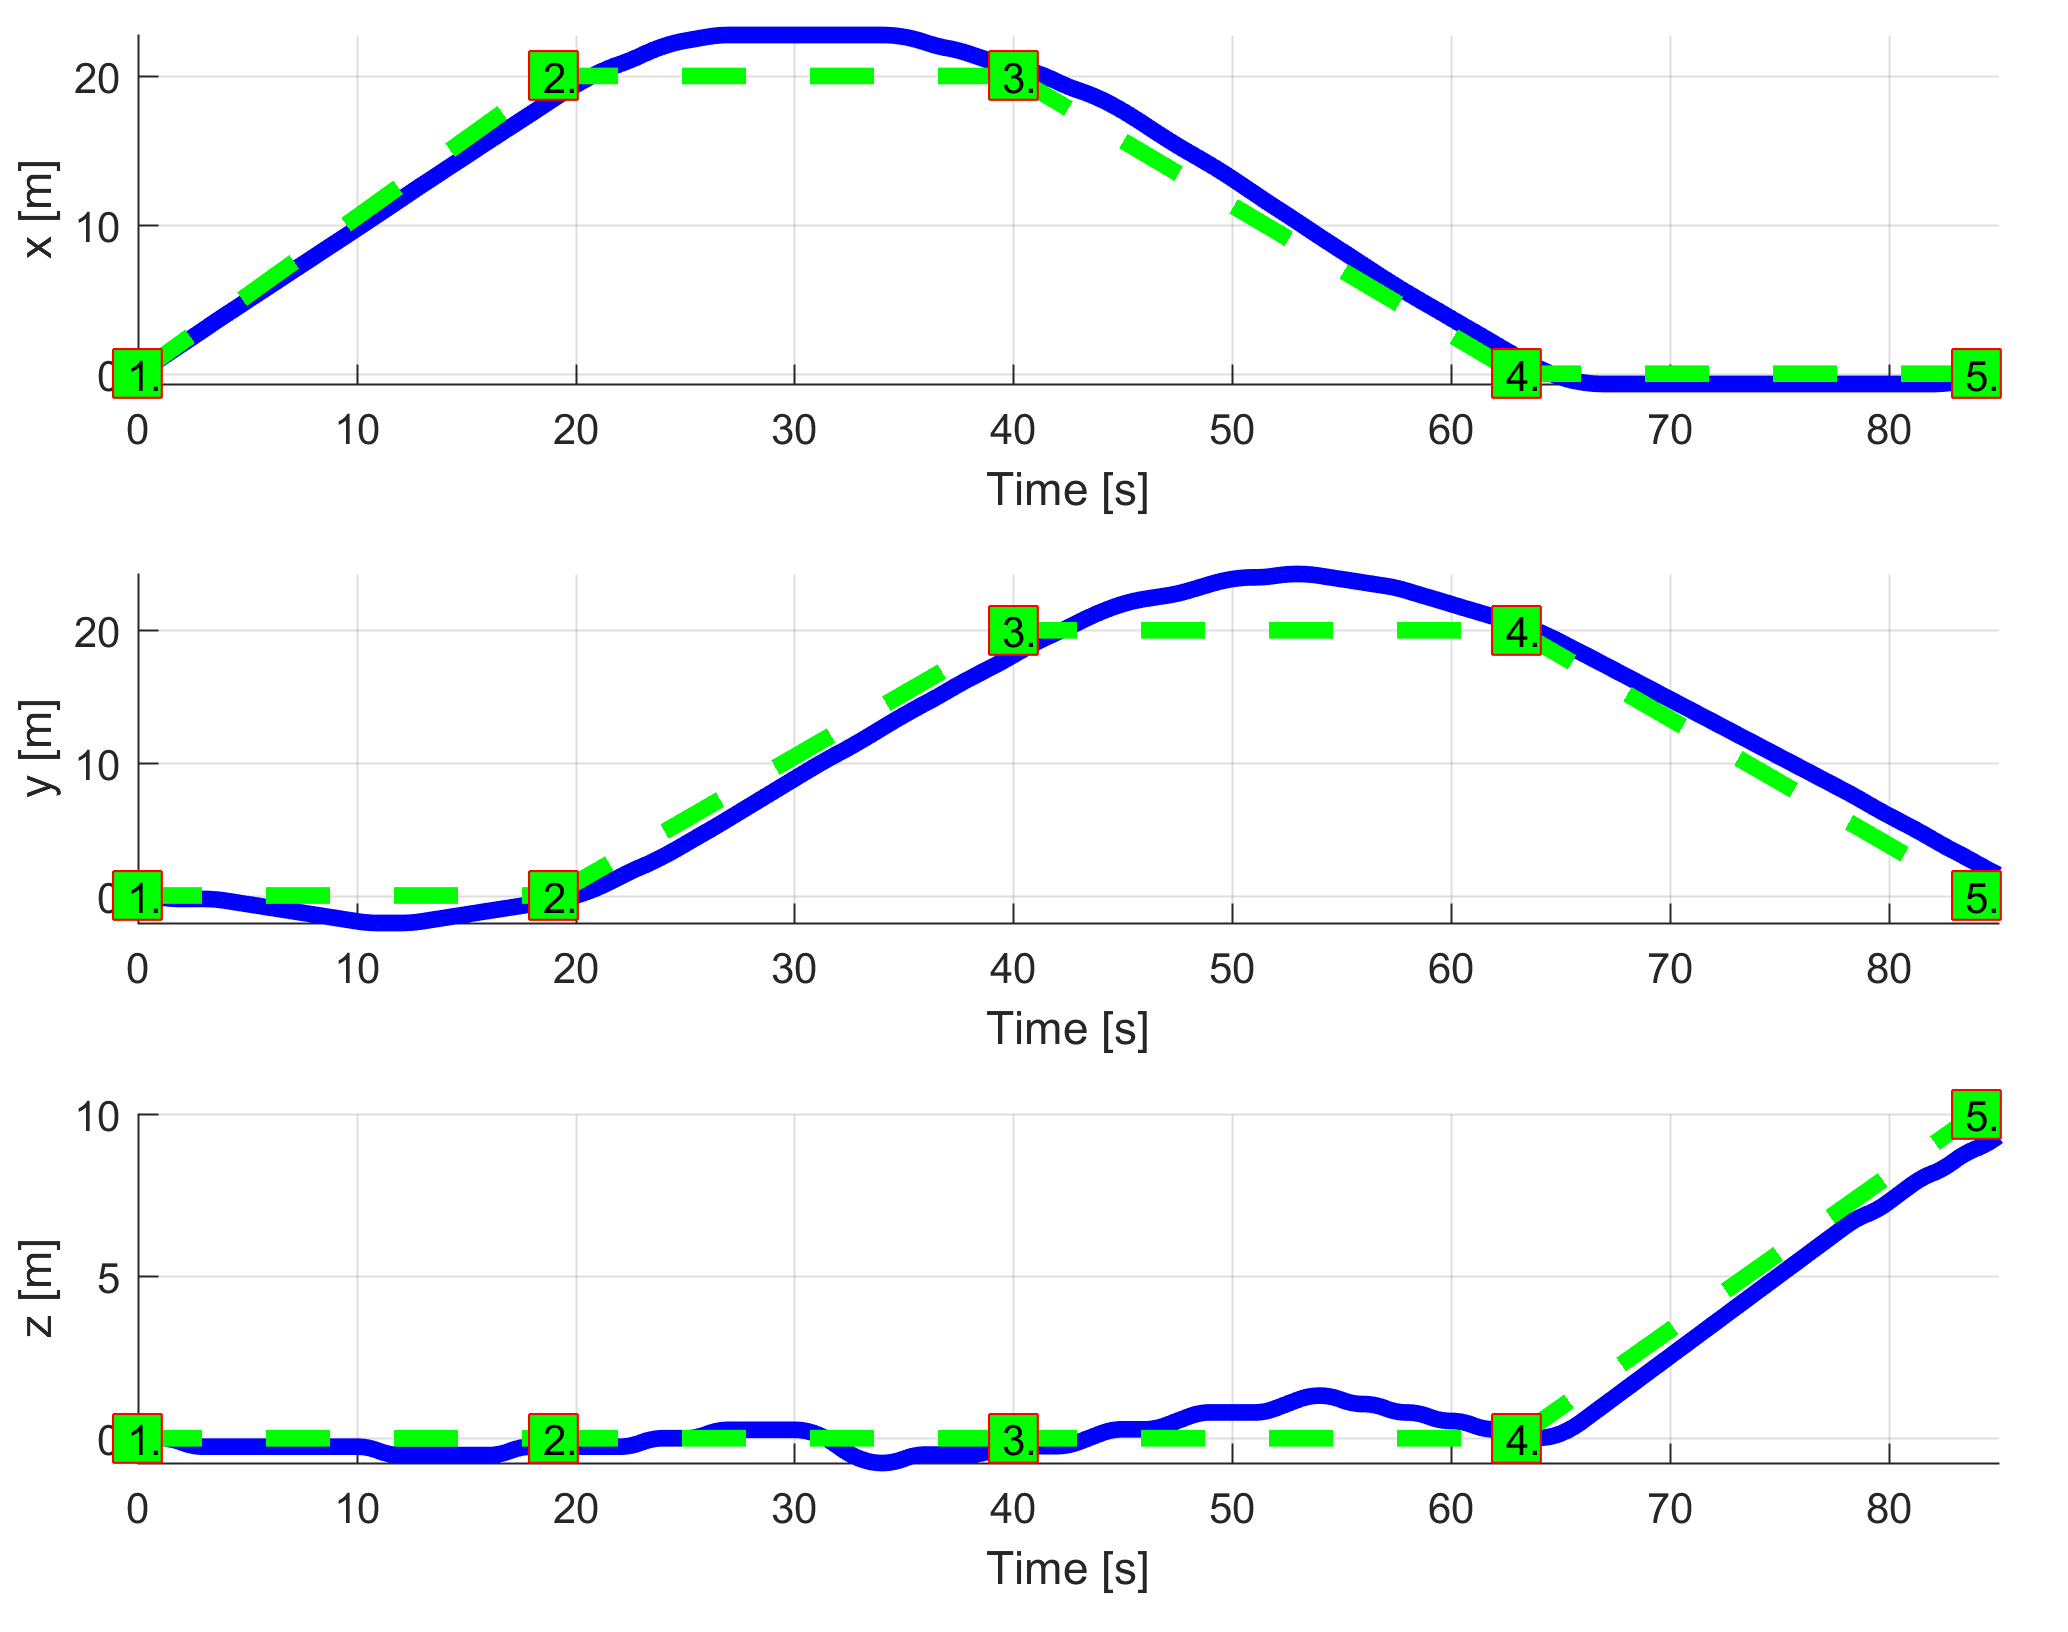
\includegraphics[width=\textwidth]{\FIGDIR/P39TrajectoryTrackingPerformance}
    \caption{Trajectory tracking performance}
    \label{fig:P39TrajectoryTrackingPerformance}
\end{figure}

\noindent\emph{Trajectory tracking performance} (fig. \ref{fig:P39TrajectoryTrackingPerformance}) displays trajectory tracking problem divided into state tracking problem of $x(t)$, $y(t)$, and $z(t)$. The ordered waypoint set $\mathscr{WP}$ is displayed as numbered green squares. The \emph{desired trajectory} $\hat{x}(t)$, $\hat{y}(t)$, and $\hat{z}(t)$ is displayed as green dashed line between waypoints. The \emph{vehicle performance} $x(t)$, $y(t)$, and $z(t)$ is displayed as blue  line. 

\emph{Overall performance} is optimal in avoidance grid $\mathscr{A}(t_i)$ and semi-optimal in joined trajectory $\mathscr{T}(x_0,B_1,\dots,B_i)$ \cite{alojzgomola2017}. This property transits from deterministic approach and its kept based on given threshold.

\section{Intruders avoidance}
\noindent \emph{Intruder avoidance} have been studied on set of avoidable intruders which maneuverability and velocity was smaller or equal to vehicle  velocity and maneuverability.
\noindent The ordered waypoint set $\mathscr{WP}$ is defined as follow:
\begin{enumerate}
    \item\emph{Starting waypoint $W_1$} - $[0,0,0]$ - not necessary, just to emphasize the local coordinate frame center
    \item\emph{Final waypoint $W_2$} - $[55,0,0]$.
\end{enumerate}


\noindent Other simulation parameters are stated like follows:
\begin{enumerate}
    \item\emph{Vehicle model $\dot{x}=f(x,u)$} is given by eq. \ref{eq:simple3ddifferentialequations}.
    \item\emph{Vehicle control $\mathscr{MA}$} is defined in section \ref{ch:movementAutomatonPredictor}.
    \item\emph{Vehicle body radius $r_b$} is given as 30 cm.
    \item\emph{Intruder horizontal spread} is estimated as $\pi/16$ [rad] for each intruder $i_k\in\mathscr{I}$.
    \item\emph{Intruder vertical spread} is estimated as $\pi/24$ [rad] for each intruder $i_k\in\mathscr{I}$.
    \item\emph{Vehicle turning radius $r_t$} is given as 2 m, this parameter impacts the decision time $t_i$ selection based on the in-veritable crash distance \cite{alojzgomola2017}.
    \item\emph{Movement automaton prediction error $E_p=(\mathscr{MA}$)} is equal to 30 cm.
    \item\emph{Safety margin $s_m$} is set to 60 cm.
    \item\emph{Avoidance grid $A(t_i) $}properties were set as follow:
    \begin{enumerate}[a.]
        \item start distance $d_s$ 0 m,
        \item end distance $d_e$ 10 m,
        \item step distance $s_d$ 1 m (10 layers),
        \item horizontal span from $\theta_s$ as $-\pi/4$ to $\theta_e$ to $\pi/4$,
        \item horizontal cell count $c_h$ as $7$,
        \item vertical span from $\varphi_s$ as $-\pi/6$ to $\varphi_e$ to $\pi/6$,
        \item vertical cell count $c_v$ as $5$ (layer count).
    \end{enumerate}
    \item\emph{Intruders set} $\mathscr{I}$ is expanding over mission time $t\in[t_s,t_e]$ and each intruder $i\in\mathscr{I}$ is detected at least at border of FOV.
\end{enumerate}

\noindent\emph{Intruder set} $\mathscr{I}$ (tab \ref{tab:intruderSet}) contains set of eight intruders $i_1,\dots,i_8$ which are discovered at mission times $t=5,\dots,40$ seconds. The intruder initial position $\vec{x}_{l}(t_D)$ is in 3D local coordinate frame given by vehicle $\vec{x}(t)$ (\ref{eq:simple3ddifferentialequations}) position and orientation at time of detection $t_D$. The same goes for intruder velocity vector $\vec{v}_{l}(t_D)$. The intruder model (\ref{eq:vehiclelinearcone}) is simple linear line model. 

The intruder intersection model $P_{O_I}(i_k,c_{i,j,k},l,b,s,\tau)$ (\ref{eq:partialProbabilitiesIntruderSummary},\ref{eq:intruderInCellProbabilityOneIntruder}) has following intersection settings:
\begin{enumerate}
    \item\emph{Linear intersection mode} $l$ set as \emph{true}.
    \item\emph{Body volume intersection mode} $b$ set as \emph{false}.
    \item\emph{Ellipsoid cone intersection mode} $s$ set as \emph{true}.
    \item\emph{Timed intersection mode} $\tau$ \emph{false}.
\end{enumerate}

\noindent\emph{Note:} All intruders are attacking vehicle from \emph{left flank} and are discovered at the margin of the FOV. All intruders have speed equal to vehicle speed $v_v$ and its 1 $ms^{-1}$.


\begin{table}[H]
    \centering
    \begin{tabular}{|c||c|c|c|}
        \hline
         Intruder & $t_D$    & $\vec{x}_{l}(t_D)$  & $\vec{v}_{l}(t_D)$ \\\hline\hline
         $i_1$    & $5$ $s$  & $[6,8,-0.5]^T$    & $[0,-1,0]^T$ \\\hline
         $i_2$    & $10$ $s$ & $[6,8,-0.5]^T$    & $[0,-1,0]^T$ \\\hline
         $i_3$    & $15$ $s$ & $[6,8,-0.5]^T$    & $[0,-1,0]^T$ \\\hline
         $i_4$    & $20$ $s$ & $[6,8,-0.5]^T$    & $[0,-1,0]^T$ \\\hline
         $i_5$    & $25$ $s$ & $[6,8,0.5]^T$     & $[0,-1,0]^T$ \\\hline
         $i_6$    & $30$ $s$ & $[6,8,0.5]^T$     & $[0,-1,0]^T$ \\\hline
         $i_7$    & $35$ $s$ & $[6,8,0.5]^T$     & $[0,-1,0]^T$ \\\hline
         $i_8$    & $40$ $s$ & $[6,8,0.5]^T$     & $[0,-1,0]^T$ \\\hline
    \end{tabular}
    \caption{Intruder set $\mathscr{I}$.}
    \label{tab:intruderSet}
\end{table}

\noindent The avoidance of intruders $i_1,i_2,\dots,i_8\in\mathscr{I}$ (tab. \ref{tab:intruderSet}). is shown in figures \ref{fig:P40FirstIntruderSideHit} and \ref{fig:P44IntruderAfterAvoidance}. where:
\begin{enumerate}
    \item\emph{Executed trajectory} (blue line) is trajectory where our vehicle flew in final, this trajectory is keeping safety property ($s_m \ge 1.2m$).
    \item\emph{Planned trajectory} (red line) - at some decision time $t_i$ in avoidance grid $\mathscr{A}(t_i)$ The most feasible trajectory to safely escape is chosen. Because of changing situation, popping up of new intruders in this case, the escape trajectory is often changed (red lines fig. \ref{fig:P41IntruderReachiSet}).
    \item\emph{Avoidance grid} (black dashed line boundary) - avoidance grid is boundary is given by vehicle position and orientation $x(t)\to \R^6$. Its depending on expected vehicle state $\hat{x}(t_i)$ at time of avoidance $t_i$.The boundary of avoidance grid $\mathscr{A(t_i=5s)}$ is in fig. \ref{fig:P39TrajectoryTrackingPerformance}. Plotting avoidance grid $\mathscr{A}$ for each time of decision $t_i$ is pointless, because it will overshadow more important information like, intruder position and planned trajectory.
    \item\emph{Decision point} (empty magenta circle) - shows when vehicle generated new avoidance grid $\mathscr{A}$ for expected state of vehicle $\hat{x}(t)$.
    \item\emph{Waypoints} (numbered green square) - direct line between two waypoint is the shortest distance to fly, the waypoints must be reached in the order.
    \item\emph{Intruder position} (full red circle) - intruder $i_k$ position at decision time $t_i$, this is intruder $i_k$ expected position. 
    \item\emph{Intruder trajectory} (linked full magenta circles) - intruder positions joined via line in previous decision times $t_{i-1},\dots,t_{i-d}$, where $t_{i-d}$ is detection time. 
\end{enumerate}
\begin{figure}[H]
    \centering
    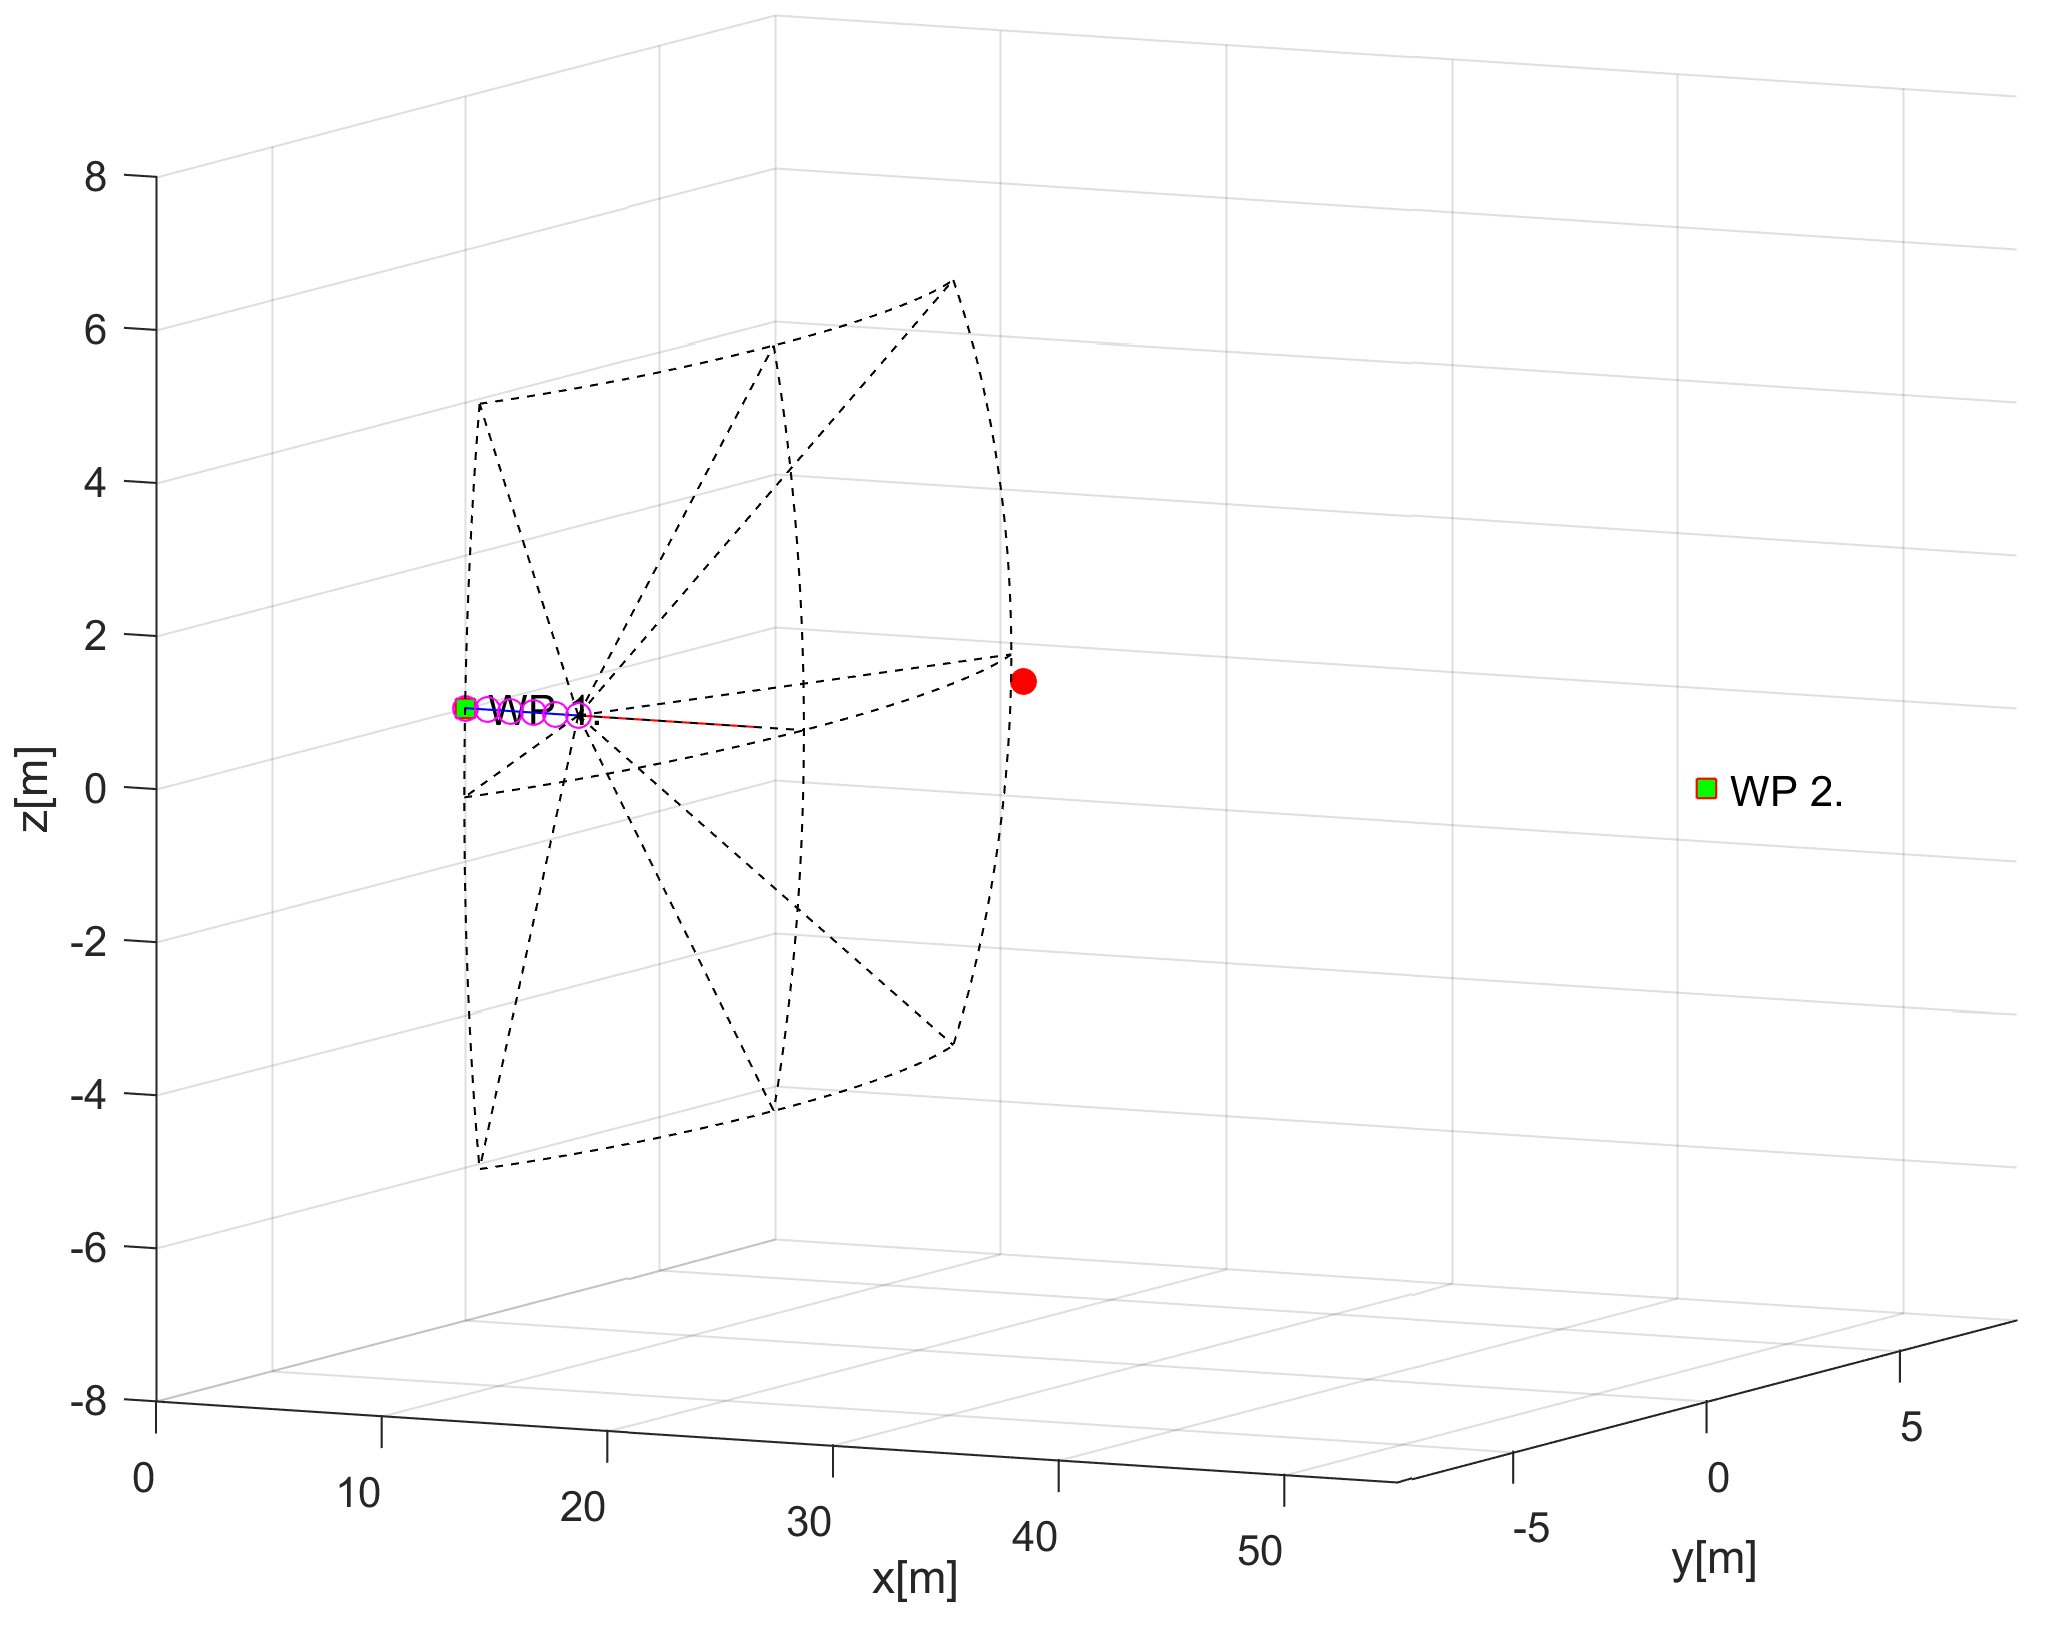
\includegraphics[width=\textwidth]{\FIGDIR/P40FirstIntruderSideHit}
    \caption{First intruder detection.}
    \label{fig:P40FirstIntruderSideHit}
\end{figure}

\noindent\emph{First intruder detection} (fig. \ref{fig:P40FirstIntruderSideHit}) shows intruder $i_1\in\mathscr{I}$ approaching vehicle (defender) from its left flank. It is guaranteed that the intruder $i_1$ and vehicle will clash each other at time $t_i+4s$, if and only if vehicle does not change course. The \emph{vehicle} is also looking for an optimal avoidance trajectory to lower the energy consumption (reminder: simple flew trajectory was used as cost function). 

\begin{figure}[H]
    \centering
    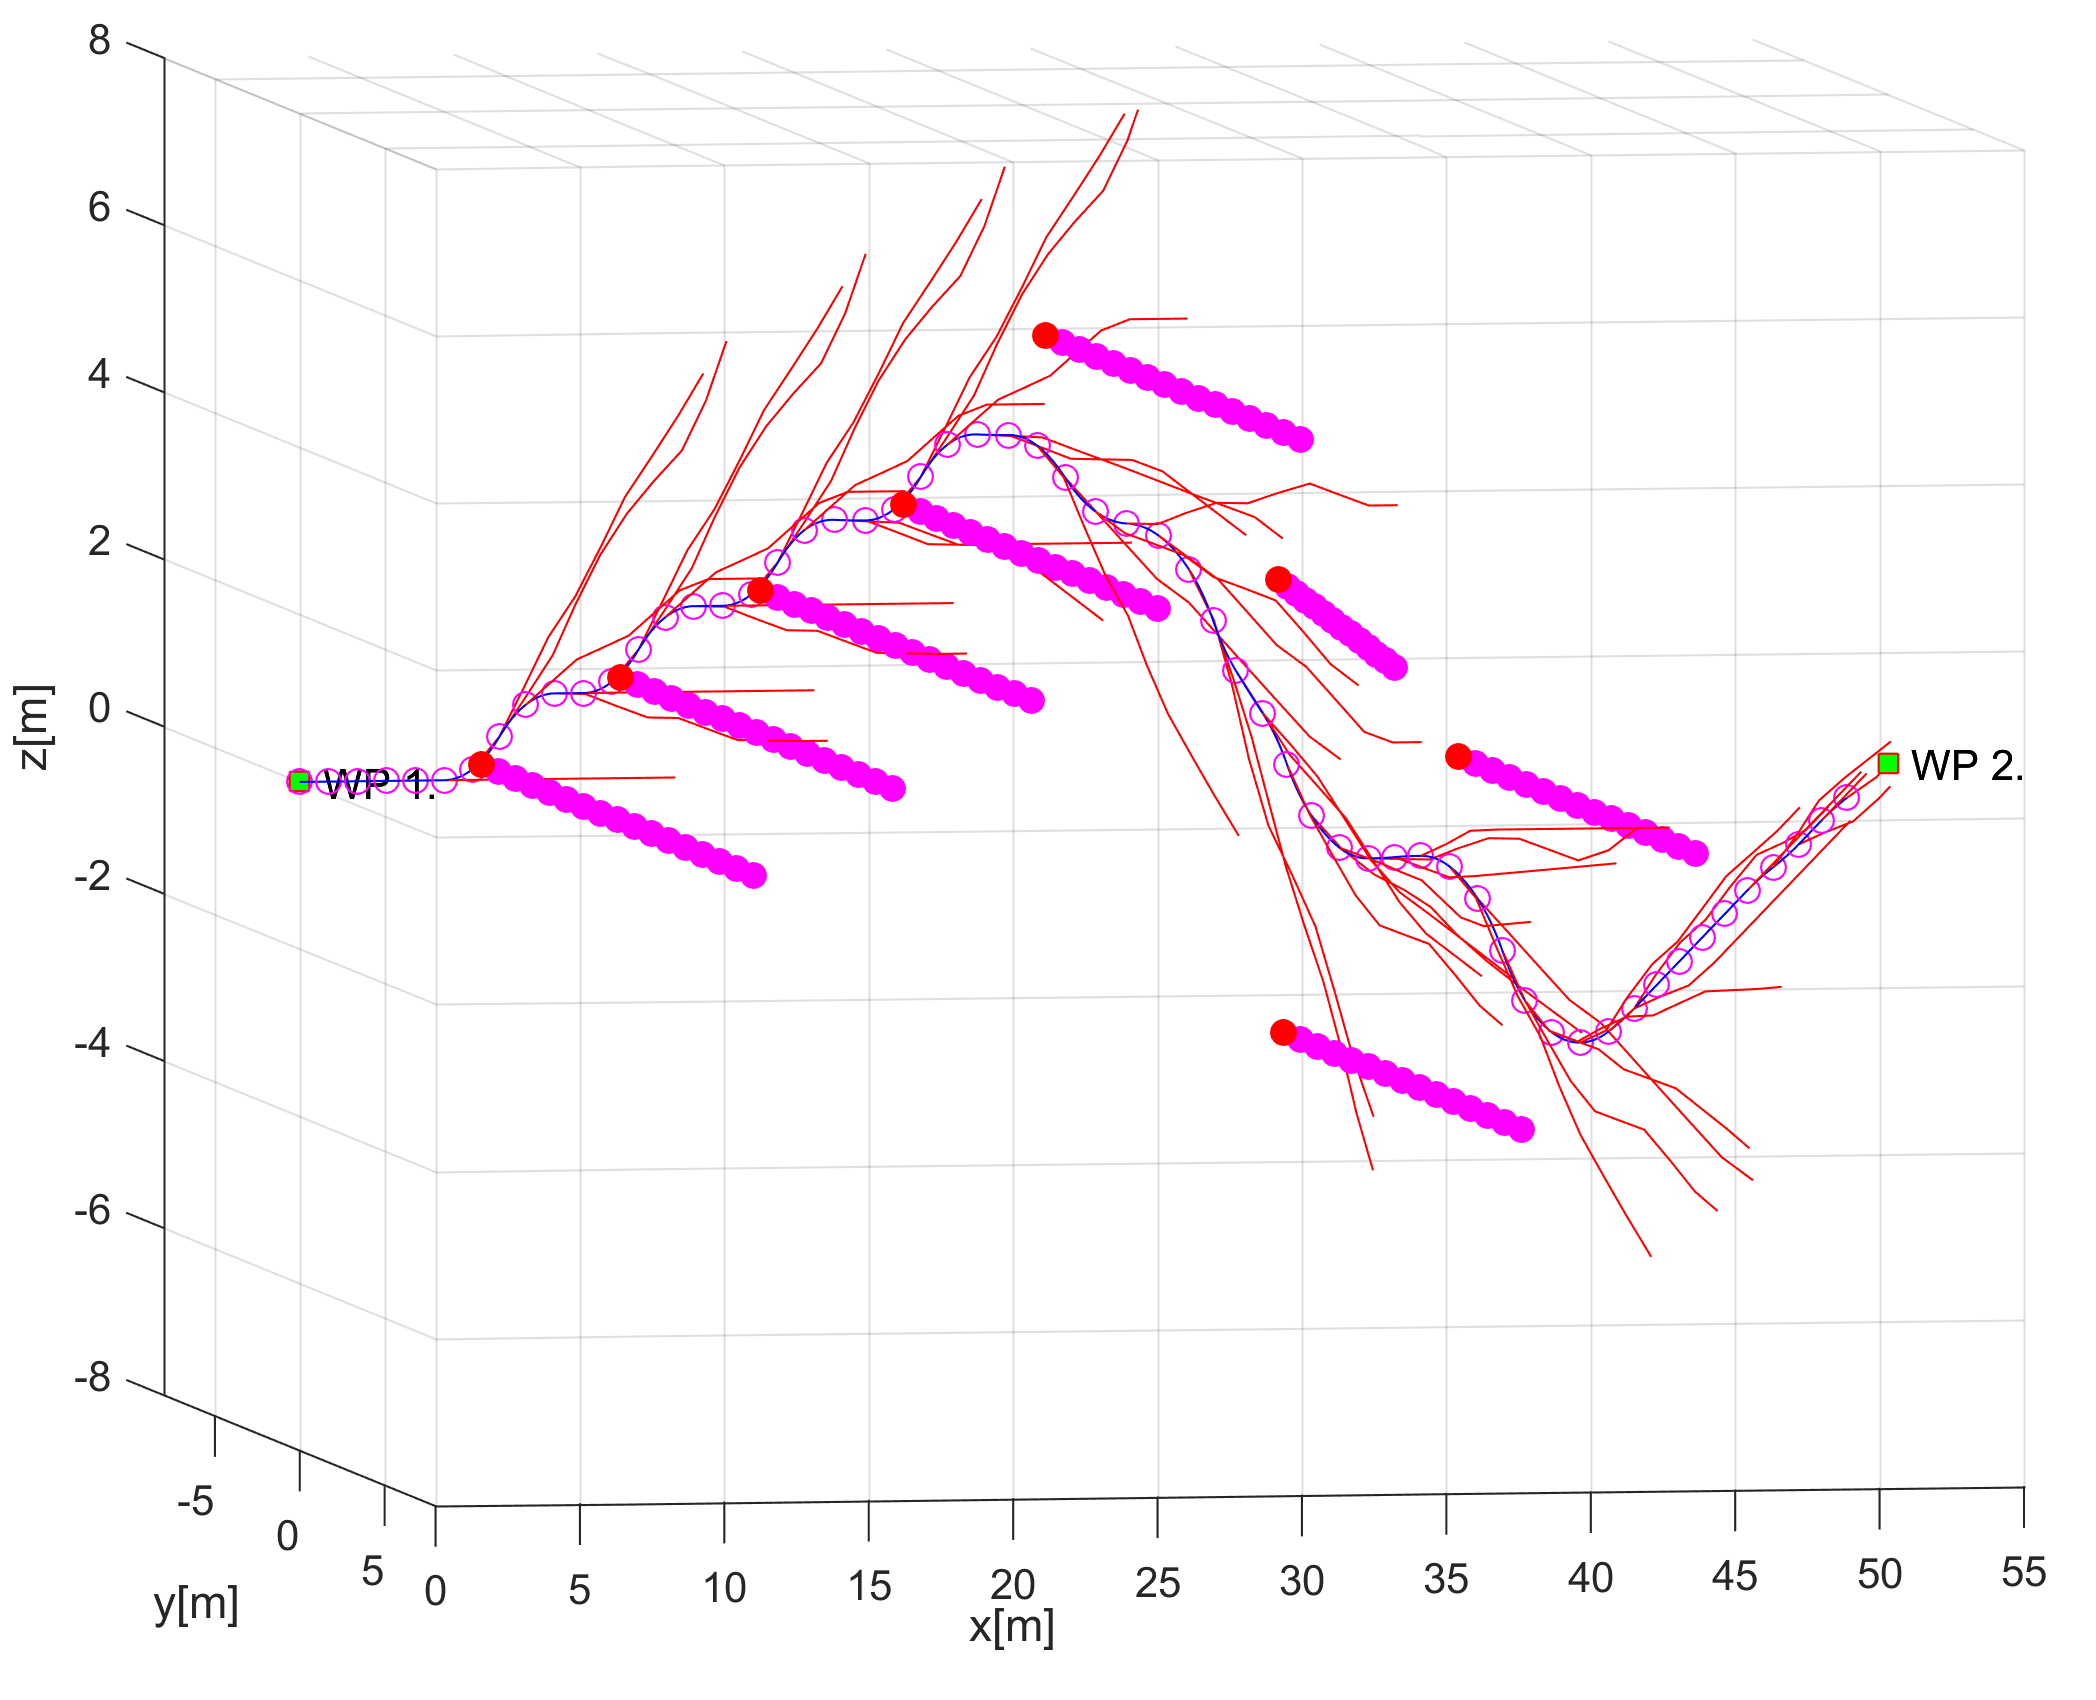
\includegraphics[width=\textwidth]{\FIGDIR/P44IntruderAfterAvoidance}
    \caption{After all intruders avoidance}
    \label{fig:P44IntruderAfterAvoidance}
\end{figure}
\noindent The final trajectory \emph{after all intruder avoidance $i_1,\dots,i_8$} is given by fig.\ref{fig:P44IntruderAfterAvoidance}. Please notice multiple trajectory change given by discovered intruders (tab. \ref{tab:intruderSet}).

\subsection{Intruder avoidance evaluation}
\noindent Due to the best knowledge of authors, all previously discussed conservative/adaptive approaches are mixing together the static and moving obstacles. There is not an single approach which separates concept of static and concept of moving obstacles (intruders) like proposed approach. 

The only important and necessary condition is safety margin, which in this case is given as: 
\begin{equation}
    s_m(i_k) = s_m + 2\times r_i(i_k)
\end{equation}
\noindent Where $s_m$ is safety margin of \emph{our vehicle}, $s_m(i_k)$ is safety margin for selected intruder. The intruder safety margin is depending on intruder body volume, in this case body volume is given by radius $r_i(i_k)$. All intruders $\forall i_k\in\mathscr{I}$ have body radius  $r_i$ equal to $60$ $cm$, therefore the safety margin for any intruder avoidance $s_m(\forall i_k)=1.2 m$.

\begin{figure}[H]
    \centering
    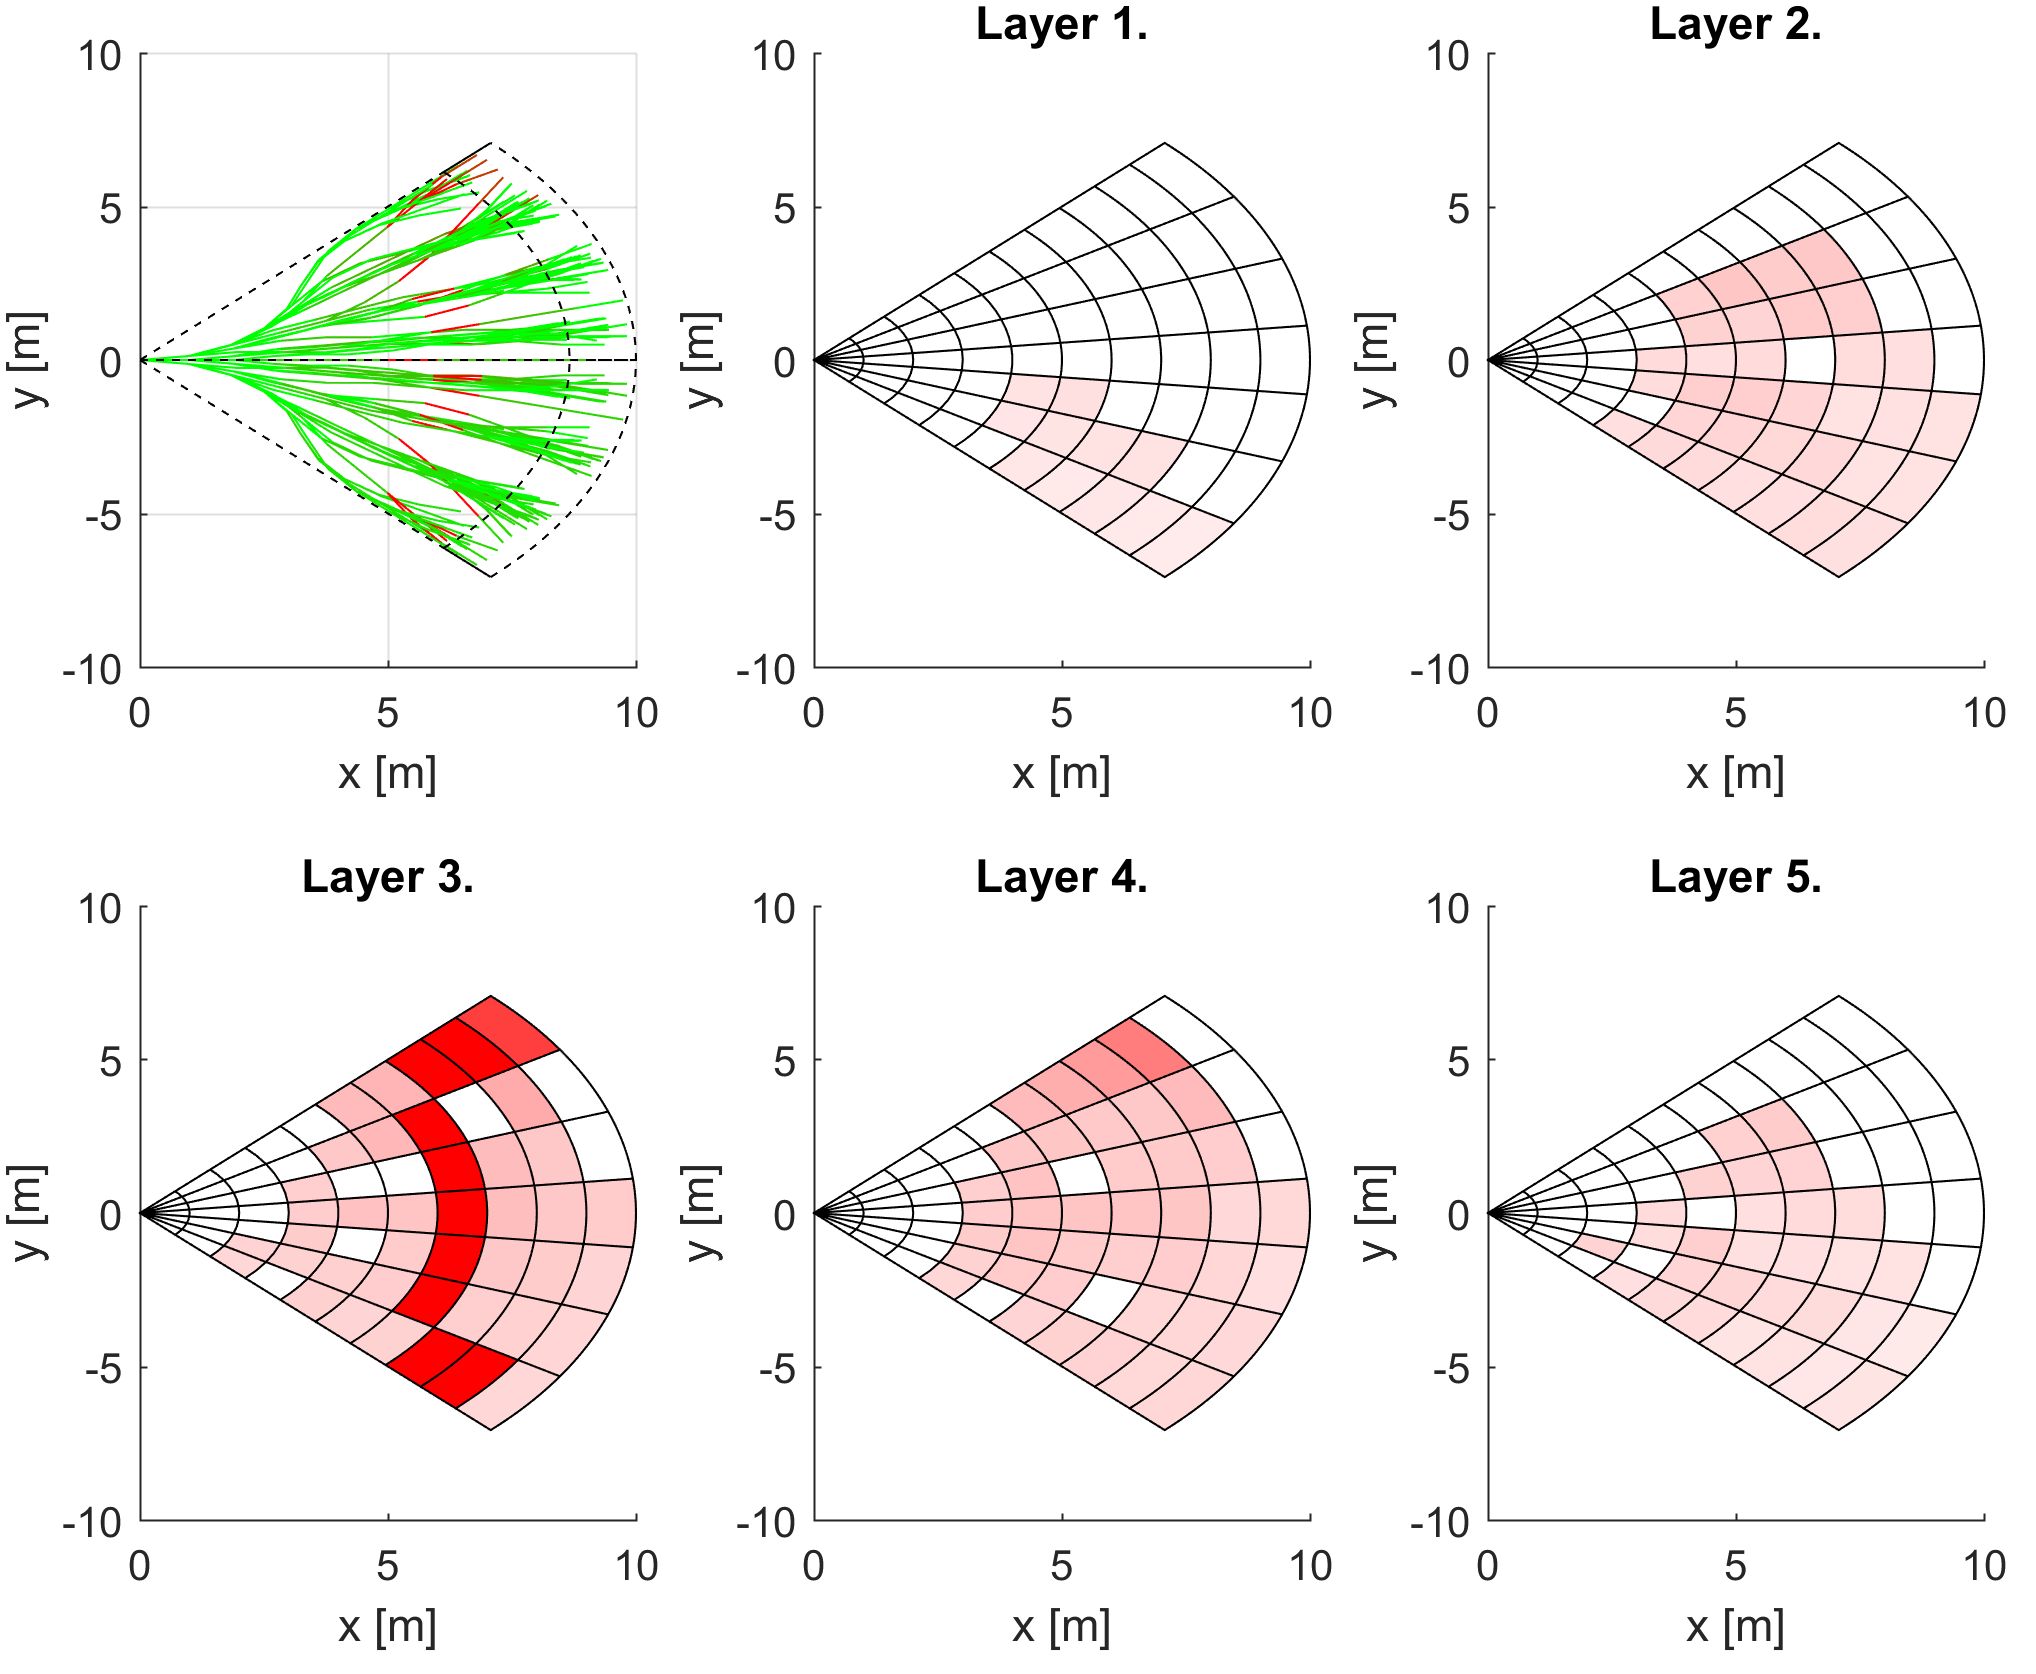
\includegraphics[width=\textwidth]{\FIGDIR/P42IntruderObstacleSpace}
    \caption{Obstacle probability after first intruder detection}
    \label{fig:P42IntruderObstacleSpace}
\end{figure}
\noindent\emph{Obstacle probability} $P_{O_I}$ (fig. \ref{fig:P42IntruderObstacleSpace}) is combination of \emph{linear intersection model} (\ref{eq:baseIntersectionProbabilityLineIntersectionType}) and \emph{conic intersection model} (\ref{eq:spreadIntruderIntersectionProbDiscrete}).

The trajectory set $\{\mathscr{T}\}\in\mathscr{R}$ is given by first sub-figure, only direct intersection cell belonging trajectories are impacted (red). Other trajectories in cones are less impacted (shades of green). 

\emph{Layer 1.} is impacted on right side and its the least impacted layer, due the lowered intruder position $z=-0.5$ ($i_1$ in tab. \ref{tab:intruderSet}). \emph{Layer 2.} contains only residuals from conic intersection and only one row on left side is free for avoidance. \emph{Layer 3.} contains direct line intersection (bright red cells) and residual conic intersection (shades of red) its one of the most impacted layers. \emph{Layer 4.} contains conic intersection residuals (shades of red), almost all layer is covered, but the probabilities of clash are rather low ($\tilde 2.5 \%$). \emph{Layer 5.} contains conic intersection residuals, it is almost symmetrical with layer 2.

\begin{figure}[H]
    \centering
    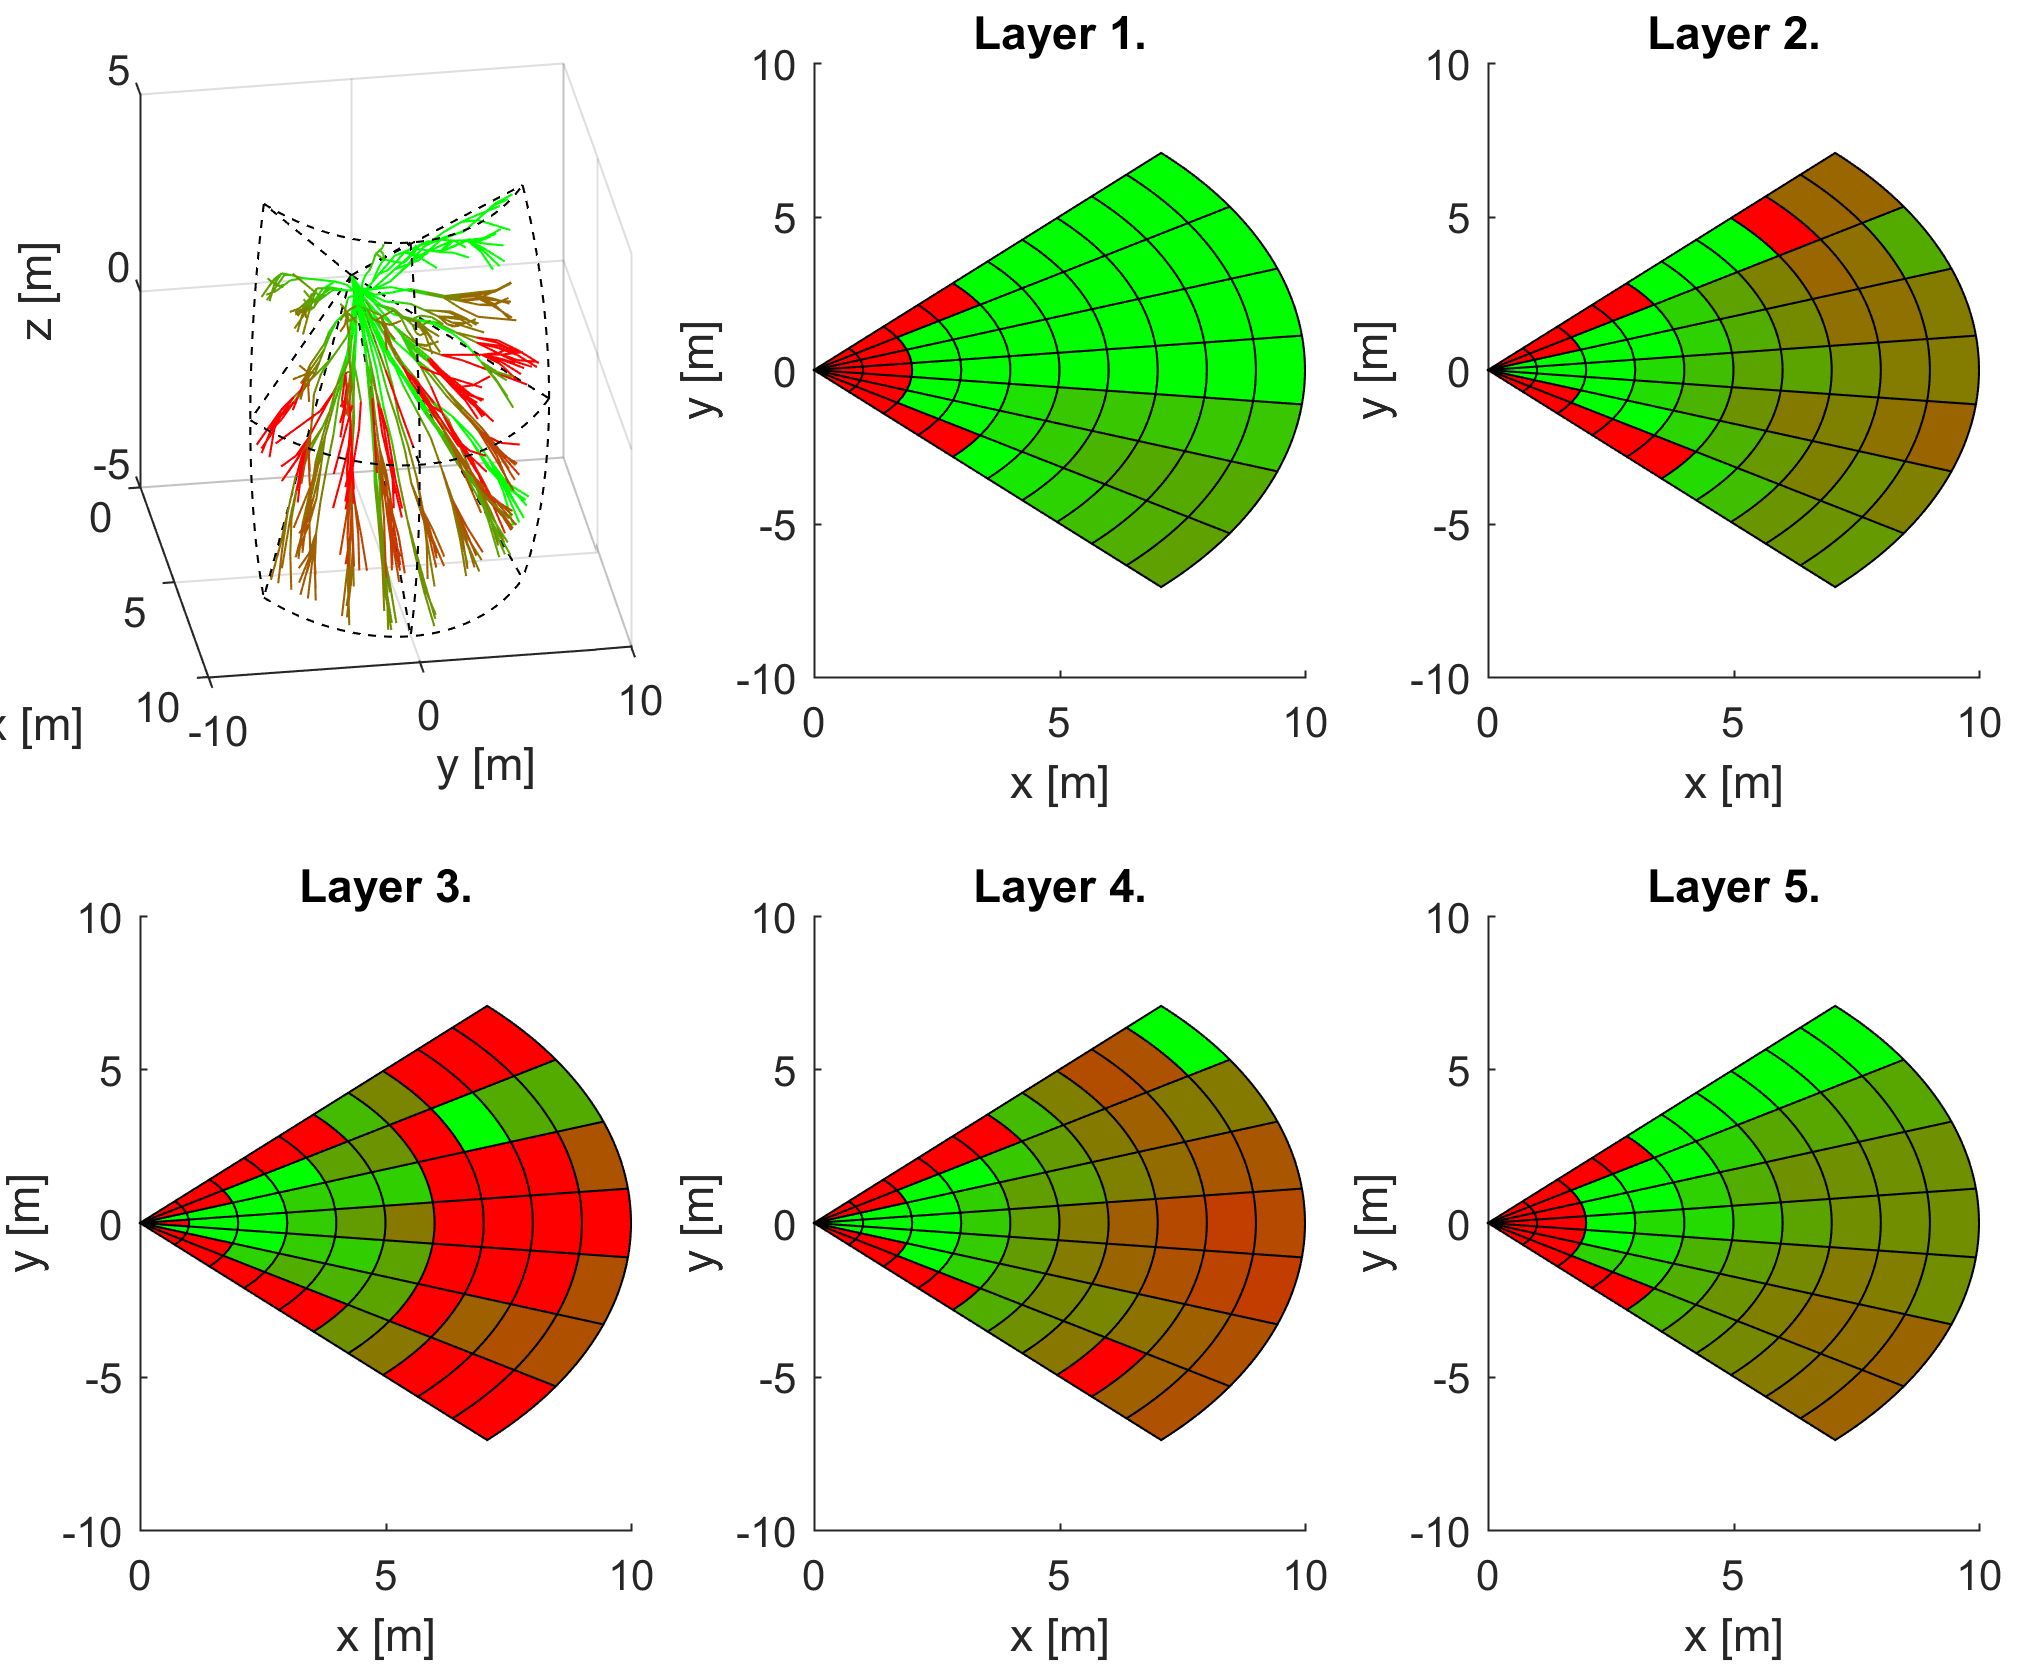
\includegraphics[width=\textwidth]{\FIGDIR/P41IntruderReachiSet}
    \caption{Reachibility probability after first intruder detection}
    \label{fig:P41IntruderReachiSet}
\end{figure}
The reach set $\mathscr{R}(\hat{x}(t_i),t_i,t_{i+1})$ for situation (fig. \ref{fig:P40FirstIntruderSideHit}) is given at top-left sub-figure  (\ref{fig:P41IntruderReachiSet}), the trajectories are colored green if reachable, brownish is semi-reachable, and red if unreachable. Please note that majority of brown trajectories are leading trough layers except intersection one (layer 3).

Reachability probability $P_R(c_{i,j,k})$ for cells $c_{i,j,k}\in\mathscr{A}(t_i)$ is varying due the different distribution of obstacle space (fig. \ref{fig:P42IntruderObstacleSpace}). The green cells are fully reachable, the brownish cells are partially reachable (more red then worse is reachability), the red cells are unreachable. \emph{Layer 1} is reachable in upper half. \emph{Layer 2.} is partially reachable on the edge, due the many routes leading trough safe \emph{layer 1}. \emph{Layer 3.} is completely blocked due the linear part of obstacle intersection ($P_{O_I}=1$). \emph{Layer 4.} is similar to \emph{layer 2.} but there are no patches of reachable space, because \emph{layer 5.} has only one reachable cell row $\mathscr{C}(1,5)$ (\ref{eq:cellrowDefinition}).


\begin{figure}[H]
    \centering
    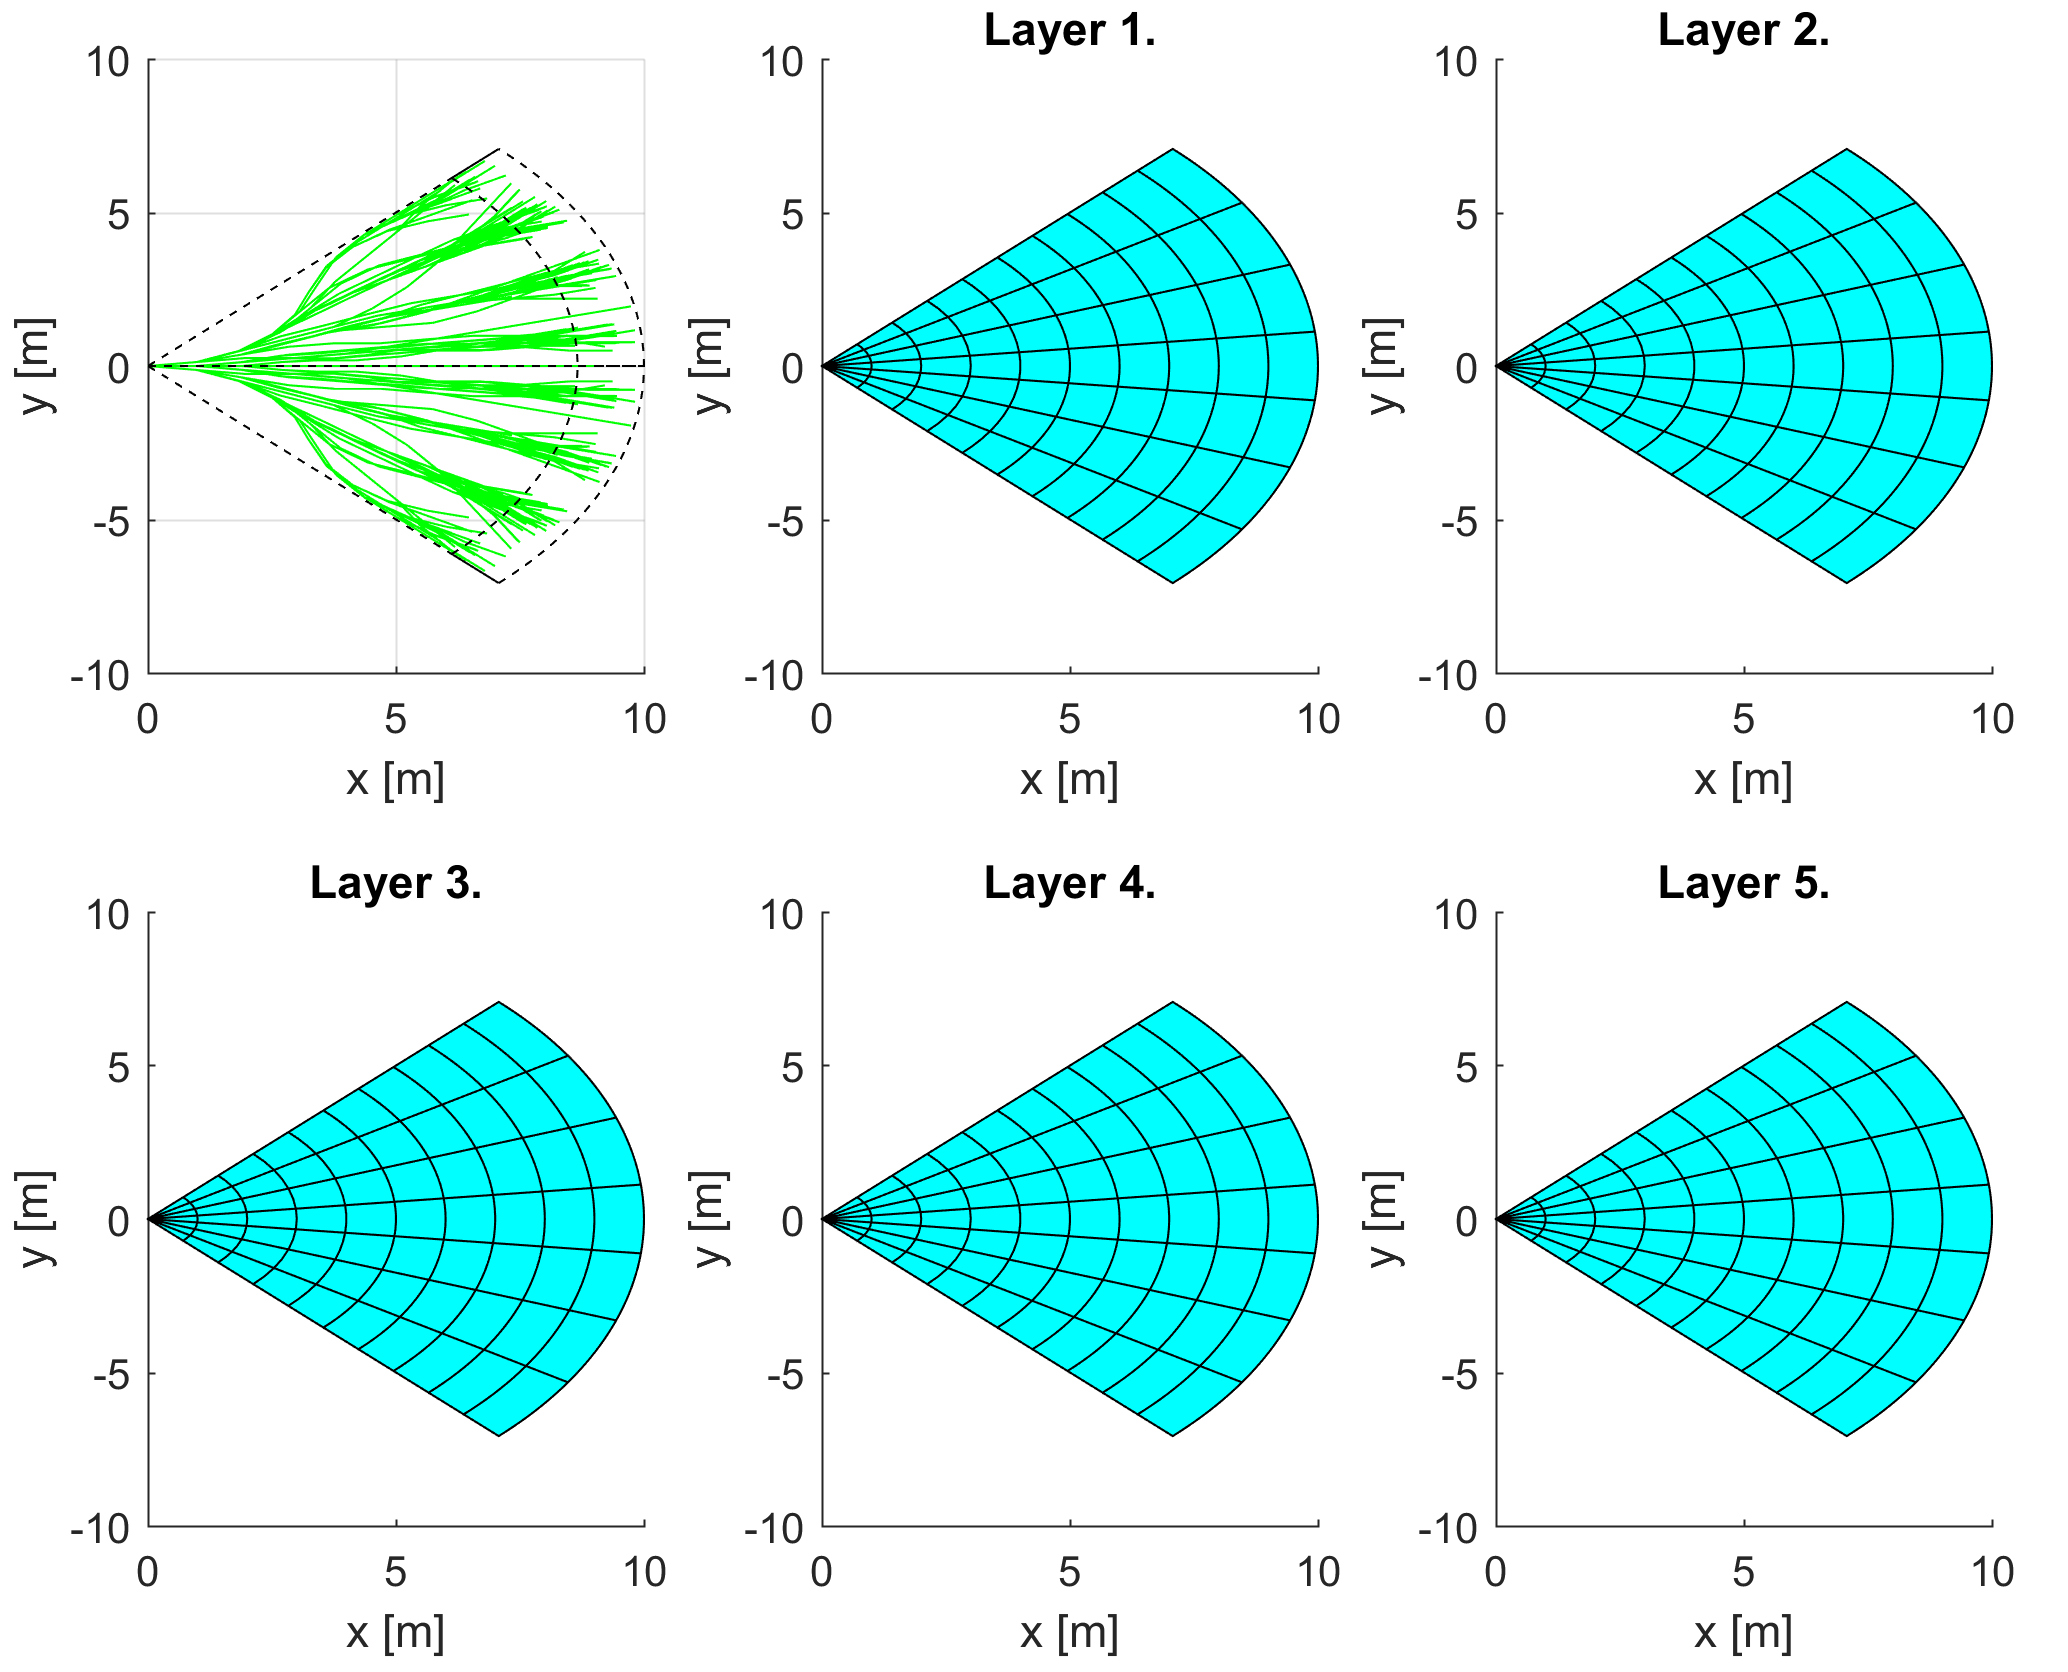
\includegraphics[width=\textwidth]{\FIGDIR/P43IntruderVisibility}
    \caption{Visibility probability after first intruder detection}
    \label{fig:P43IntruderVisibility}
\end{figure}
\noindent The visibility probability $P_V(C_{i,j,k})$ is equal to one for all cells, because there is no real hindrance in visibility. The intruder obstacle probability $P_{O_I}$ can be accounted as a sort of virtual obstacle to be avoided. 

Concept of \emph{virtual obstacles} is very strong and it can be used to implement virtual barriers around object of significant importance.

\emph{Intruder collision distance} $c_D(t)$ is a minimal distance between any intruder and vehicle trajectory at given time snapshot $\tau$. For fixed time $\tau$, there exist a set of intruder positions like follow:
\begin{equation}\label{eq:setOfIntrudersPositionsFixedTime}
    \mathscr{I}_P(\tau)=\left\{\vec{p}\in\R^3:p=\vec{x}(\tau)\to\R^3,\vec{x}(\tau)\in i_k, i_k\in \mathscr{I}(\tau)\right\}
\end{equation}
Where $\vec{p}$ is point in global coordinates, created by projection of intruder state $\vec{x}(\tau)$ to \emph{global coordinate frame} $\R^3$ for each intruder $i_k$ in detected intruders set $\mathscr{I}(\tau)$.

\emph{The closest intruder} $i_c$ in detected intruder set $\mathscr{I}(\tau)$ for fixed time $\tau$ is given as:
\begin{equation}
    i_c(\tau,\vec{x}_v(\tau))=i_k\in\mathscr{I}:\min_{\forall \vec{p}_i\in\mathscr{I}_P(\tau), \vec{x}_v(\tau)}\left\{\norm{\vec{p}_i-\left( \vec{x}_v(\tau)\to\R^3\right)}\right\}
\end{equation}
Where the $\vec{x}_v(\tau)\to\R^3$ is projection of our vehicle state $\vec{x}_v$ at fixed time $\tau$ projected to global coordinate frame $\mathscr{R}^3$, the closest intruder $i_c$ is selected based on vehicle position and set of intruders positions $\mathscr{I}_P(\tau)$ (\ref{eq:setOfIntrudersPositionsFixedTime}). The norm $\norm{\cdot}$ is standard euclidean. 

\emph{Collision distance} function $c_D(t)$ is calculated for steepest time $\tau$ in mission time frame $[t_s,t_e]$, where $t_s$ is mission start time and $t_e$ mission end time. For fixed time $\tau$ the minimal distance between vehicle position $\vec{x}_v(\tau)\to\R^3$ in global coordinate frame $\R^3$, and intruder position $\vec{p}_i$ from intruder set $\mathscr{I}_P(\tau)$ used as crash distance $c_d$ for particular $\tau$. The collision distance is formulated in following equation:
\begin{equation}
    c_D(t)=\left\{c_d\in\R: c_d=\min_{\forall \vec{p}_i\in\mathscr{I}_P(\tau), \vec{x}_v(\tau)}\left\{\norm{\vec{p}_i-\left( \vec{x}_v(\tau)\to\R^3\right)}\right\}, \forall \tau \in [t_s,t_e]\right\}
\end{equation}

\begin{figure}[H]
    \centering
    \includegraphics[width=\textwidth]{\FIGDIR/P45IntruderDistanceEvolution}
    \caption{Intruder collision distance $c_d(t)$ evolution.}
    \label{fig:P45IntruderDistanceEvolution}
\end{figure}

\noindent \emph{Intruder collision distance $c_d(t)$ evolution} (\ref{fig:P45IntruderDistanceEvolution}) shows that the necessary condition $c_D(t)\ge s_m (1.2 m)$ holds. \emph{Green line} shows evolution over time. \emph{Green full circles} are marking the closest intruder $i_k\in\mathscr{I}(t)$, defined in table \ref{tab:intruderSet}. The time starts at $5s$ when first intruder is detected. The evolution of $c_D(t)$ reflects how intruders were popping out and tried to collide with our vehicle. The closest intruder was $i_4$ whom achieves distance of $136 cm$.

\chapter{Conclusion and Future work}\label{ch:07Conclusion}
\paragraph{Conceptual problem formulation} is introduced in chapter \ref{ch:01Concept}. Where related work and goals are main focus, the goals have been fulfilled to some extent and some aspects needs additional work. 

\paragraph{The \emph{data fusion problem}} has been formulated in \ref{ch:02DataFusionProblem}, the three questions of \emph{visibility, reachability, and obstacle probability} have been confronted with deterministic approach shortcomings (sec. \ref{sec:deterministicApproachShortcommings}), where problem of \emph{LiDAR density} (fig. \ref{fig:P01CountOfLiDARHits}), \emph{map and detected obstacles fusion} (fig. \ref{fig:P02OvershadowedMapobstacle}), \emph{Intruder behaviour} (fig. \ref{fig:P03AdversaryProbabilitySpread}), and \emph{safety of passing trajectories} (fig. \ref{fig:P04SafetyOfPassingTrajectories}) have been opened.

\paragraph{The state of art} have been discussed in chapter \ref{03StateOfArt}. This chapter is taken from most parts \cite{alojzgomola2017}. It introduces the notion of UAV model in continuous time (\ref{eq:nonlinearsystem}) and in discrete time (\ref{eq:Discretegenericuavmodel}) The key concepts of reach sets are given in section \ref{s:ReachSets}. The reach set used further in $\mathscr{R}(\hat{x},t_i,t_{i_1})$ (\ref{eq:basicReachSetDefinition}), is point based reach set with restricted control. Movement automaton $\mathscr{MA}$ concept is introduced in section \ref{sec:movement automaton}, by definition \ref{def:movementAutomaton}. \emph{Movement automaton prediction stability} is given by definition \ref{def:maPredictionStability}. \emph{Movement automaton Lyapunov stability} is proven in section \ref{s:maLyapunov}. The other important properties, like \emph{controllability, robustness, observability} have been proven in \cite{frazzoli2000trajectory}.

\paragraph{The control framework based on reach sets} have been introduced in \cite{alojzgomola2017}. The complex topology scheme and communication is omitted in conclusion, only key modules for this work will be discussed. \emph{Obstacle avoidance} in terms of data fusion with dynamic obstacle sets $\mathscr{O}_D$, $O_M$, originating from various data sources $\mathscr{S}=\{s_1,s_2,\dots,s_k\}, k\in\N$. Movement constraints are mainly given by static uncharted obstacles and non-cooperative intruders. The main focus is on \emph{data fusion}. Usually multiple layer control concept is used. Control concept used for this work is in fig. \ref{fig:controlConceptIntro}.
\begin{figure}[H]
    \centering
    \includegraphics[width=.95\linewidth]{\FIGDIR/72_Control_Concept.png}
    \caption{Decision frame $\mathscr{D}(0)$.}
    \label{fig:controlConceptIntro}
\end{figure}

\noindent \emph{Event based control} module is responsible for high level decisions and mission execution. This module generates high level input commands which are optimal to given criterion. \emph{Event based control} consist from following artifacts:
\begin{enumerate}
    \item \emph{Sensor fusion} - fuses data from sensor system with observed system state $\hat{x}$, outputs detected obstacles $o_i\in\mathscr{O}$.
    \item \emph{Mission plan} - contains mission plan $\mathscr{WP}$, determines navigation goal waypoint $\mathscr{WP}_g$.
    \item \emph{Rule engine} - determines additional constraints for avoidance grid $\mathscr{A}(t_i)$, determines escape goal in avoidance grid $c_{i,j,k}$.
    \item \emph{Avoidance grid} - responsible for optimal path planning in partially known space, consumes observed system state $\hat{x}(t)$, rule engine decisions $r_i(\tau)$, obstacle set $o_i\in\mathscr{O}$ and goal waypoint $\mathscr{WP}_i$, produces avoidance command chain $B_p \in \mathbb{M}^k$.
\end{enumerate}

\emph{Discrete control} module is responsible for processing high level movement command chain $B_p \in \mathbb{M}^k$. It is implemented as special type of open hybrid automaton, movement automaton $\mathscr{MA}$. 

\emph{Continuous control} module is interfaces from \emph{avoidance} system via the movement automaton. The same is achieved with \emph{sensor fusion} module which is interfacing the sensor network $\mathscr{S}$ and avoidance grid $\mathscr{A}(t_i)$.

\paragraph{Problem of data fusion} is formulated in chapter \ref{ch:04ProblemFormulation}, outlining important \emph{general data fusion algorithm} proposal, section \ref{sec:general algorithm}. The identified probabilities and input artifacts are summarized in eq. \ref{eq:mainRatingInputs}. The \emph{main fusion algorithm} is proposed in eq. \ref{eq:mainRatingCalculation}. The new definition of \emph{reachability probability} $P_R$ bounded to trajectory $\mathscr{T}(x_0,B)\in\mathscr{R}$ have been established by definition \ref{def:ReachibilityProbabilityForTrajectory}, furthermore projected into cell $c_{i,j,k}\in\mathscr{A}$ reachability probability established by definition \ref{def:cellReachibilityProbability}.

\paragraph{Reduced reach set} calculation have been introduced due the calculation complexity of probabilistic distribution over full reach set. Concept of \emph{coverage ratio} $C_R$ (\ref{eq:reachSetCoverageRatio}) which considers \emph{trajectory footprint} (def. \ref{def:trajectoryFootprint}, \ref{def:trajectoryFootprintSet}). The \emph{constrained expansion procedure} (sec \ref{susbsec:ConstrainedExpansionProcedure}) have been developed to improve estimated reach set calculation. Three new procedures to reach set $\mathscr{R}(\hat{x},t_i,t_{i+1})$ have been developed:
\begin{enumerate}
    \item Chaotic reach set approximation (sec. \ref{s:chaoticApproximationReachSet}).
    \item Harmonic reach set approximation (sec. \ref{s:harmonicApproximationReachSet}).
    \item Combined reach set approximation (considered in testing) (sec .\ref{s:combinedReachSetApproximation}).
\end{enumerate}

\paragraph{Important results} are linked to research proposal goals:

\noindent\emph{Goal 1.: Universal interface for vehicle sensors} have been introduced in section \ref{sec:general algorithm}.

\noindent\emph{Goal 2.: Probabilistic model for avoidance grid} have been summarized in topics:
\begin{enumerate}
    \item\emph{Intruder intersection model} (sec. \ref{sec:intruderIntersectionModel}) introduces the concept of intruder intersection with avoidance grid. The notable are boundaries for cell entry (\ref{eq:cellEntryTime}) and cell leave time (\ref{eq:cellLeaveTime}) which enables to take time into account when calculating probability (\ref{eq:intruderIntersectionProbability}). Concept of base intersection probability have been defined for following intersection modes:
    \begin{enumerate}[a.]
        \item linear intersection model (\ref{eq:baseIntersectionProbabilityLineIntersectionType}),
        \item vehicle body volume intersection model (\ref{eq:baseIntersectionProbabilityBallIntersectionType}),
        \item conic spread intersection model (\ref{eq:spreadIntruderIntersectionProb}).
    \end{enumerate}
    \noindent Then \emph{general producible intersection model} (\ref{eq:intruderInCellProbabilityOneIntruder}) of one intruder $i\in\mathscr{I}$ has been defined combining the previously mentioned intersection modes of base probabilities and time constraints (\ref{eq:partialProbabilitiesIntruderSummary}). The intruder obstacle probability for single cell $c_{i,j,k}\in\mathscr{A}(t_i)$ and multiple intruders $i \in \mathscr{I}(\tau)$ has been given by (\ref{eq:intruderInCellProbability}).
    
    \item\emph{Detected obstacle probability} generic model for multiple sensors $s_k\in\mathscr{S}$ has been given by eq. \ref{eq:detectedObstacleProbability}. \textit{LiDAR hit formula} (\ref{eq:lidarHitFormula}) has been created for simple homogeneous rotary LiDAR sensor.
    
    \item\emph{Visibility probability} for sensor network $\mathscr{S}$ has been defined in eq. \ref{eq:FinalVisibilityProbability}.
    
    \item\emph{Map obstacle probability} is defined as combination of visibility and raw map obstacle probability (\ref{eq:finalMapObstacleProbability}).
\end{enumerate}

\emph{Goal 3.: Data fusion procedure} is proposed in section \ref{sec:general algorithm}.

\emph{Goal 4.: Comparison of probabilistic and deterministic approach} have been simulated in section \ref{sec:staticObstacleAvoidanceSimulation}. Detailed comparison with results from deterministic approach \cite{alojzgomola2017} are given in section \ref{sec:probabilisticModelEvaluation}. \emph{Avoidance performance} is compared in section \ref{sec:avoidancePerformacne}.

\paragraph{Future work} on probabilistic approach is mainly in partition of sensor fusion. Currently the sensor fusion for LiDAR and ADS-B have been proposed, but there is more ranging sensors which are not coherence with avoidance grid like LiDAR. 

\emph{Sensor fusion priority problem:} Vehicle can be equipped with various cooperative and non-cooperative sensors $s_1,s_2,\dots,s_4\in\mathscr{S}$. Which have some overlapped areas and some precision. It would be necessary to develop \emph{prioritized sensor fusion}, complex outline of this problem in deterministic context have been given by \cite{xiong2002multi}.

\paragraph{Reusable components for deterministic approach}: Probabilistic approach have introduced concepts of \emph{coverage ratio} $C_R$ and \emph{reduced reach set approximation}. These results can be used to reduce reach set complexity and improve scalability of deterministic approach \cite{alojzgomola2017}.

\emph{The intruder intersection model} can be reused in deterministic approach, where the step function to asset the reachability of cell. 

\bibliography{thesis}
%\include{08Annex}
\end{document}
